\documentclass{book}
\usepackage[a4paper,top=2.5cm,bottom=2.5cm,left=2.5cm,right=2.5cm]{geometry}
\usepackage{makeidx}
\usepackage{natbib}
\usepackage{graphicx}
\usepackage{multicol}
\usepackage{float}
\usepackage{listings}
\usepackage{color}
\usepackage{ifthen}
\usepackage[table]{xcolor}
\usepackage{textcomp}
\usepackage{alltt}
\usepackage{ifpdf}
\ifpdf
\usepackage[pdftex,
            pagebackref=true,
            colorlinks=true,
            linkcolor=blue,
            unicode
           ]{hyperref}
\else
\usepackage[ps2pdf,
            pagebackref=true,
            colorlinks=true,
            linkcolor=blue,
            unicode
           ]{hyperref}
\usepackage{pspicture}
\fi
\usepackage[utf8]{inputenc}
\usepackage{mathptmx}
\usepackage[scaled=.90]{helvet}
\usepackage{courier}
\usepackage{sectsty}
\usepackage{amssymb}
\usepackage[titles]{tocloft}
\usepackage{doxygen}
\lstset{language=C++,inputencoding=utf8,basicstyle=\footnotesize,breaklines=true,breakatwhitespace=true,tabsize=4,numbers=left }
\makeindex
\setcounter{tocdepth}{3}
\renewcommand{\footrulewidth}{0.4pt}
\renewcommand{\familydefault}{\sfdefault}
\hfuzz=15pt
\setlength{\emergencystretch}{15pt}
\hbadness=750
\tolerance=750
\begin{document}
\hypersetup{pageanchor=false,citecolor=blue}
\begin{titlepage}
\vspace*{7cm}
\begin{center}
{\Large Steeriously \\[1ex]\large 0.\-1 }\\
\vspace*{1cm}
{\large Generated by Doxygen 1.8.2}\\
\vspace*{0.5cm}
{\small Sun Dec 10 2017 18:36:39}\\
\end{center}
\end{titlepage}
\clearemptydoublepage
\pagenumbering{roman}
\tableofcontents
\clearemptydoublepage
\pagenumbering{arabic}
\hypersetup{pageanchor=true,citecolor=blue}
\chapter{Steeriously}
\label{index}\hypertarget{index}{}Steeriously. A dead-\/simple pure C++ library for adding steering behaviors to your game and multimedia entities. \par
All credit goes to Mat Buckland for writing \char`\"{}\-Programming A\-I by Example\char`\"{} and providing such great steering code. \par
All source is derived from \char`\"{}\-Programming A\-I by Example\char`\"{}.\par
 \par
I can't recommend the book enough -\/ you can buy the book here\-: \par
\href{http://www.amazon.com/Programming-Example-Wordware-Developers-Library/dp/1556220782/ref=sr_1_1?ie=UTF8&qid=1446057032&sr=8-1&keywords=programming+ai+by+example}{\tt Programming A\-I by Example} \par
 \par
Steeriously has one humble goal -\/ to make steering behavior accessible and fun to program. \par
One way to achieve this is by redesigning the original code to expose a more general purpose A\-P\-I. \par
 \par
Tutorials and examples for using this library are available at\-: \par
 \par
\href{http://pushbuttonreceivecode.com}{\tt pushbuttonreceivecode.\-com }\begin{DoxyVersion}{Version}
0.\-1 
\end{DoxyVersion}
\begin{DoxyAuthor}{Author}
Mark Richards 
\end{DoxyAuthor}
\begin{DoxyDate}{Date}
12/9/2017 \par
 
\end{DoxyDate}
\begin{DoxyParagraph}{===================== L\-I\-C\-E\-N\-S\-E =====================}
The zlib/libpng License \par
 Copyright (c) 2017 Mark Richards \par
 \par
 This software is provided 'as-\/is', without any express or implied warranty. In no event will the authors be held liable for any damages arising from the use of this software. Permission is granted to anyone to use this software for any purpose, including commercial applications, and to alter it and redistribute it freely, subject to the following restrictions\-: \par

\begin{DoxyEnumerate}
\item The origin of this software must not be misrepresented; you must not claim that you wrote the original software. If you use this software in a product, an acknowledgment in the product documentation would be appreciated but is not required.
\item Altered source versions must be plainly marked as such, and must not be misrepresented as being the original software.
\item This notice may not be removed or altered from any source distribution. 
\end{DoxyEnumerate}
\end{DoxyParagraph}

\chapter{Namespace Index}
\section{Namespace List}
Here is a list of all documented namespaces with brief descriptions\-:\begin{DoxyCompactList}
\item\contentsline{section}{\hyperlink{namespacesteer}{steer} \\*All steering functions are templated for easy application to objects inheriting from \hyperlink{classsteer_1_1_agent}{Agent}. Because of this, it is easy to add into any type of design -\/ be it a class hierarchy or a more advanced data structure or system (such as an entity component system). All functions return a steer\-::steer\-::\-Vector2 that can be used to calculate a force with which the entity should be moved given each type of behavior. Combine each calculated force with a weight (any scalar value -\/ but keep it sane or behavior could become strange). Simply multiply each weight, or weights, by the force generated by each behavior's return value to fine-\/tune it. In addition to the steering functions themselves, this file contains various utilities used by them to perform their work }{\pageref{namespacesteer}}{}
\end{DoxyCompactList}

\chapter{Hierarchical Index}
\section{Class Hierarchy}
This inheritance list is sorted roughly, but not completely, alphabetically\-:\begin{DoxyCompactList}
\item \contentsline{section}{steer\-:\-:Agent}{\pageref{classsteer_1_1_agent}}{}
\begin{DoxyCompactList}
\item \contentsline{section}{steer\-:\-:Arrive\-Component}{\pageref{classsteer_1_1_arrive_component}}{}
\item \contentsline{section}{steer\-:\-:Evade\-Component}{\pageref{classsteer_1_1_evade_component}}{}
\item \contentsline{section}{steer\-:\-:Flee\-Component}{\pageref{classsteer_1_1_flee_component}}{}
\item \contentsline{section}{steer\-:\-:Flocking\-Component}{\pageref{classsteer_1_1_flocking_component}}{}
\item \contentsline{section}{steer\-:\-:Hide\-Component}{\pageref{classsteer_1_1_hide_component}}{}
\item \contentsline{section}{steer\-:\-:Interpose\-Component}{\pageref{classsteer_1_1_interpose_component}}{}
\item \contentsline{section}{steer\-:\-:Offset\-Pursuit\-Component}{\pageref{classsteer_1_1_offset_pursuit_component}}{}
\item \contentsline{section}{steer\-:\-:Path\-Following\-Component}{\pageref{classsteer_1_1_path_following_component}}{}
\item \contentsline{section}{steer\-:\-:Pursuit\-Component}{\pageref{classsteer_1_1_pursuit_component}}{}
\item \contentsline{section}{steer\-:\-:Seek\-Component}{\pageref{classsteer_1_1_seek_component}}{}
\item \contentsline{section}{steer\-:\-:Super\-Component}{\pageref{classsteer_1_1_super_component}}{}
\item \contentsline{section}{steer\-:\-:Wander\-Component}{\pageref{classsteer_1_1_wander_component}}{}
\end{DoxyCompactList}
\item \contentsline{section}{steer\-:\-:Behavior\-Parameters}{\pageref{structsteer_1_1_behavior_parameters}}{}
\item \contentsline{section}{steer\-:\-:Matrix2\-D}{\pageref{classsteer_1_1_matrix2_d}}{}
\item \contentsline{section}{steer\-:\-:Path}{\pageref{classsteer_1_1_path}}{}
\item \contentsline{section}{steer\-:\-:Sphere\-Obstacle}{\pageref{classsteer_1_1_sphere_obstacle}}{}
\item \contentsline{section}{steer\-:\-:Vector2}{\pageref{structsteer_1_1_vector2}}{}
\item \contentsline{section}{steer\-:\-:Vector\-Math}{\pageref{classsteer_1_1_vector_math}}{}
\item \contentsline{section}{steer\-:\-:Wall}{\pageref{classsteer_1_1_wall}}{}
\end{DoxyCompactList}

\chapter{Class Index}
\section{Class List}
Here are the classes, structs, unions and interfaces with brief descriptions\-:\begin{DoxyCompactList}
\item\contentsline{section}{\hyperlink{classsteer_1_1_agent}{steer\-::\-Agent} \\*The invisible, but highly necessary, automaton which drives your $\ast$game entity/graphical representation's motion. Getters and Setters are provided, $\ast$however it will always be easier to just use the data -\/ since it is all public }{\pageref{classsteer_1_1_agent}}{}
\item\contentsline{section}{\hyperlink{classsteer_1_1_arrive_component}{steer\-::\-Arrive\-Component} \\*An example implementation of the arrive steering behavior. The agent will seek the target with a dampened arrival }{\pageref{classsteer_1_1_arrive_component}}{}
\item\contentsline{section}{\hyperlink{structsteer_1_1_behavior_parameters}{steer\-::\-Behavior\-Parameters} \\*Data table with default values used to define variables for guiding steerable objects (agents) }{\pageref{structsteer_1_1_behavior_parameters}}{}
\item\contentsline{section}{\hyperlink{classsteer_1_1_evade_component}{steer\-::\-Evade\-Component} \\*An example implementation of the evasion steering behavior. The agent will flee from the target while predicting it's trajectory }{\pageref{classsteer_1_1_evade_component}}{}
\item\contentsline{section}{\hyperlink{classsteer_1_1_flee_component}{steer\-::\-Flee\-Component} \\*An example implementation of the flee steering behavior. The agent will flee from the target when it enters its threat range }{\pageref{classsteer_1_1_flee_component}}{}
\item\contentsline{section}{\hyperlink{classsteer_1_1_flocking_component}{steer\-::\-Flocking\-Component} \\*An example implementation of the flocking steering behavior. The agent will interact with other members of the flock utilizing alignment, separation, cohesion, and wandering behaviors }{\pageref{classsteer_1_1_flocking_component}}{}
\item\contentsline{section}{\hyperlink{classsteer_1_1_hide_component}{steer\-::\-Hide\-Component} \\*An example implementation of the hiding steering behavior }{\pageref{classsteer_1_1_hide_component}}{}
\item\contentsline{section}{\hyperlink{classsteer_1_1_interpose_component}{steer\-::\-Interpose\-Component} \\*An example implementation of the interpose steering behavior }{\pageref{classsteer_1_1_interpose_component}}{}
\item\contentsline{section}{\hyperlink{classsteer_1_1_matrix2_d}{steer\-::\-Matrix2\-D} \\*A class for 2\-D matrices and related operations }{\pageref{classsteer_1_1_matrix2_d}}{}
\item\contentsline{section}{\hyperlink{classsteer_1_1_offset_pursuit_component}{steer\-::\-Offset\-Pursuit\-Component} \\*An example implementation of the offset pursuit steering behavior }{\pageref{classsteer_1_1_offset_pursuit_component}}{}
\item\contentsline{section}{\hyperlink{classsteer_1_1_path}{steer\-::\-Path} \\*Class providing the necessary structure for path following behavior }{\pageref{classsteer_1_1_path}}{}
\item\contentsline{section}{\hyperlink{classsteer_1_1_path_following_component}{steer\-::\-Path\-Following\-Component} \\*An example implementation of the path following steering behavior }{\pageref{classsteer_1_1_path_following_component}}{}
\item\contentsline{section}{\hyperlink{classsteer_1_1_pursuit_component}{steer\-::\-Pursuit\-Component} \\*An example implementation of the pursuit steering behavior }{\pageref{classsteer_1_1_pursuit_component}}{}
\item\contentsline{section}{\hyperlink{classsteer_1_1_seek_component}{steer\-::\-Seek\-Component} \\*An example implementation of the seek steering behavior }{\pageref{classsteer_1_1_seek_component}}{}
\item\contentsline{section}{\hyperlink{classsteer_1_1_sphere_obstacle}{steer\-::\-Sphere\-Obstacle} \\*Class to aid in obstacle avoidance routine }{\pageref{classsteer_1_1_sphere_obstacle}}{}
\item\contentsline{section}{\hyperlink{classsteer_1_1_super_component}{steer\-::\-Super\-Component} \\*An example implementation of the an agent with every steering behavior implemented }{\pageref{classsteer_1_1_super_component}}{}
\item\contentsline{section}{\hyperlink{structsteer_1_1_vector2}{steer\-::\-Vector2} \\*A 2\-D vector struct used in many steering calculations }{\pageref{structsteer_1_1_vector2}}{}
\item\contentsline{section}{\hyperlink{classsteer_1_1_vector_math}{steer\-::\-Vector\-Math} \\*Stateless \hyperlink{classsteer_1_1_vector_math}{Vector\-Math} class utilizing static methods to manipulate vectors. \par
Copies of \hyperlink{structsteer_1_1_vector2}{Vector2} are cheap, therefore all functions are \char`\"{}pass by value\char`\"{} at this time }{\pageref{classsteer_1_1_vector_math}}{}
\item\contentsline{section}{\hyperlink{classsteer_1_1_wall}{steer\-::\-Wall} \\*A class for constructing 2\-D walls for wall avoidance behaviors }{\pageref{classsteer_1_1_wall}}{}
\item\contentsline{section}{\hyperlink{classsteer_1_1_wander_component}{steer\-::\-Wander\-Component} \\*An example implementation of the wander steering behavior }{\pageref{classsteer_1_1_wander_component}}{}
\end{DoxyCompactList}

\chapter{Namespace Documentation}
\hypertarget{namespacesteer}{\section{steer Namespace Reference}
\label{namespacesteer}\index{steer@{steer}}
}


All steering functions are templated for easy application to objects inheriting from \hyperlink{classsteer_1_1_agent}{Agent}. Because of this, it is easy to add into any type of design -\/ be it a class hierarchy or a more advanced data structure or system (such as an entity component system). All functions return a steer\-::steer\-::\-Vector2 that can be used to calculate a force with which the entity should be moved given each type of behavior. Combine each calculated force with a weight (any scalar value -\/ but keep it sane or behavior could become strange). Simply multiply each weight, or weights, by the force generated by each behavior's return value to fine-\/tune it. In addition to the steering functions themselves, this file contains various utilities used by them to perform their work.  


\subsection*{Classes}
\begin{DoxyCompactItemize}
\item 
class \hyperlink{classsteer_1_1_agent}{Agent}
\begin{DoxyCompactList}\small\item\em The invisible, but highly necessary, automaton which drives your $\ast$game entity/graphical representation's motion. Getters and Setters are provided, $\ast$however it will always be easier to just use the data -\/ since it is all public. \end{DoxyCompactList}\item 
struct \hyperlink{structsteer_1_1_behavior_parameters}{Behavior\-Parameters}
\begin{DoxyCompactList}\small\item\em Data table with default values used to define variables for guiding steerable objects (agents). \end{DoxyCompactList}\item 
class \hyperlink{classsteer_1_1_arrive_component}{Arrive\-Component}
\begin{DoxyCompactList}\small\item\em An example implementation of the arrive steering behavior. The agent will seek the target with a dampened arrival. \end{DoxyCompactList}\item 
class \hyperlink{classsteer_1_1_evade_component}{Evade\-Component}
\begin{DoxyCompactList}\small\item\em An example implementation of the evasion steering behavior. The agent will flee from the target while predicting it's trajectory. \end{DoxyCompactList}\item 
class \hyperlink{classsteer_1_1_flee_component}{Flee\-Component}
\begin{DoxyCompactList}\small\item\em An example implementation of the flee steering behavior. The agent will flee from the target when it enters its threat range. \end{DoxyCompactList}\item 
class \hyperlink{classsteer_1_1_flocking_component}{Flocking\-Component}
\begin{DoxyCompactList}\small\item\em An example implementation of the flocking steering behavior. The agent will interact with other members of the flock utilizing alignment, separation, cohesion, and wandering behaviors. \end{DoxyCompactList}\item 
class \hyperlink{classsteer_1_1_hide_component}{Hide\-Component}
\begin{DoxyCompactList}\small\item\em An example implementation of the hiding steering behavior. \end{DoxyCompactList}\item 
class \hyperlink{classsteer_1_1_interpose_component}{Interpose\-Component}
\begin{DoxyCompactList}\small\item\em An example implementation of the interpose steering behavior. \end{DoxyCompactList}\item 
class \hyperlink{classsteer_1_1_offset_pursuit_component}{Offset\-Pursuit\-Component}
\begin{DoxyCompactList}\small\item\em An example implementation of the offset pursuit steering behavior. \end{DoxyCompactList}\item 
class \hyperlink{classsteer_1_1_path_following_component}{Path\-Following\-Component}
\begin{DoxyCompactList}\small\item\em An example implementation of the path following steering behavior. \end{DoxyCompactList}\item 
class \hyperlink{classsteer_1_1_pursuit_component}{Pursuit\-Component}
\begin{DoxyCompactList}\small\item\em An example implementation of the pursuit steering behavior. \end{DoxyCompactList}\item 
class \hyperlink{classsteer_1_1_seek_component}{Seek\-Component}
\begin{DoxyCompactList}\small\item\em An example implementation of the seek steering behavior. \end{DoxyCompactList}\item 
class \hyperlink{classsteer_1_1_super_component}{Super\-Component}
\begin{DoxyCompactList}\small\item\em An example implementation of the an agent with every steering behavior implemented. \end{DoxyCompactList}\item 
class \hyperlink{classsteer_1_1_wander_component}{Wander\-Component}
\begin{DoxyCompactList}\small\item\em An example implementation of the wander steering behavior. \end{DoxyCompactList}\item 
class \hyperlink{classsteer_1_1_matrix2_d}{Matrix2\-D}
\begin{DoxyCompactList}\small\item\em A class for 2\-D matrices and related operations. \end{DoxyCompactList}\item 
class \hyperlink{classsteer_1_1_path}{Path}
\begin{DoxyCompactList}\small\item\em Class providing the necessary structure for path following behavior. \end{DoxyCompactList}\item 
class \hyperlink{classsteer_1_1_sphere_obstacle}{Sphere\-Obstacle}
\begin{DoxyCompactList}\small\item\em Class to aid in obstacle avoidance routine. \end{DoxyCompactList}\item 
struct \hyperlink{structsteer_1_1_vector2}{Vector2}
\begin{DoxyCompactList}\small\item\em A 2\-D vector struct used in many steering calculations. \end{DoxyCompactList}\item 
class \hyperlink{classsteer_1_1_vector_math}{Vector\-Math}
\begin{DoxyCompactList}\small\item\em Stateless \hyperlink{classsteer_1_1_vector_math}{Vector\-Math} class utilizing static methods to manipulate vectors. \par
Copies of \hyperlink{structsteer_1_1_vector2}{Vector2} are cheap, therefore all functions are \char`\"{}pass by value\char`\"{} at this time. \end{DoxyCompactList}\item 
class \hyperlink{classsteer_1_1_wall}{Wall}
\begin{DoxyCompactList}\small\item\em A class for constructing 2\-D walls for wall avoidance behaviors. \end{DoxyCompactList}\end{DoxyCompactItemize}
\subsection*{Typedefs}
\begin{DoxyCompactItemize}
\item 
\hypertarget{namespacesteer_ac624bd4d8a4c5c8cec38cb037962696c}{typedef signed char \hyperlink{namespacesteer_ac624bd4d8a4c5c8cec38cb037962696c}{Int8}}\label{namespacesteer_ac624bd4d8a4c5c8cec38cb037962696c}

\begin{DoxyCompactList}\small\item\em $<$ Useful typedefs for signed/unsigned integers. \end{DoxyCompactList}\item 
\hypertarget{namespacesteer_a15b608712afd89174dd4bbb50c35ab70}{typedef unsigned char {\bfseries Uint8}}\label{namespacesteer_a15b608712afd89174dd4bbb50c35ab70}

\item 
\hypertarget{namespacesteer_a32f62ea8587b74f423b3112a633a3c8f}{typedef signed short {\bfseries Int16}}\label{namespacesteer_a32f62ea8587b74f423b3112a633a3c8f}

\item 
\hypertarget{namespacesteer_a203b74e59ae2cd122624a0f8fdd0ac69}{typedef unsigned short {\bfseries Uint16}}\label{namespacesteer_a203b74e59ae2cd122624a0f8fdd0ac69}

\item 
\hypertarget{namespacesteer_a1e0f7ba830c800fa6d940c46b8b1aa36}{typedef signed int {\bfseries Int32}}\label{namespacesteer_a1e0f7ba830c800fa6d940c46b8b1aa36}

\item 
\hypertarget{namespacesteer_aaf5daf8c35e087eb70c1d5378f62617f}{typedef unsigned int {\bfseries Uint32}}\label{namespacesteer_aaf5daf8c35e087eb70c1d5378f62617f}

\item 
\hypertarget{namespacesteer_a09ece6b46d4f0fbc8d22248cdf350c00}{typedef signed long long {\bfseries Int64}}\label{namespacesteer_a09ece6b46d4f0fbc8d22248cdf350c00}

\item 
\hypertarget{namespacesteer_a3d3437f640c793384ae68c4b453a6f21}{typedef unsigned long long \hyperlink{namespacesteer_a3d3437f640c793384ae68c4b453a6f21}{Uint64}}\label{namespacesteer_a3d3437f640c793384ae68c4b453a6f21}

\begin{DoxyCompactList}\small\item\em Useful constants for minimum and maximum values. \end{DoxyCompactList}\end{DoxyCompactItemize}
\subsection*{Enumerations}
\begin{DoxyCompactItemize}
\item 
enum \hyperlink{namespacesteer_afe6e72f8f8088962727051501181acbe}{behavior\-Type} \{ \\*
{\bfseries none} = 0x00000, 
{\bfseries seek} = 0x00002, 
{\bfseries flee} = 0x00004, 
{\bfseries arrive} = 0x00008, 
\\*
{\bfseries wander} = 0x00010, 
{\bfseries cohesion} = 0x00020, 
{\bfseries separation} = 0x00040, 
{\bfseries alignment} = 0x00080, 
\\*
{\bfseries obstacle\-Avoidance} = 0x00100, 
{\bfseries wall\-Avoidance} = 0x00200, 
{\bfseries follow\-Path} = 0x00400, 
{\bfseries pursuit} = 0x00800, 
\\*
{\bfseries evade} = 0x01000, 
{\bfseries interpose} = 0x02000, 
{\bfseries hide} = 0x04000, 
{\bfseries flock} = 0x08000, 
\\*
{\bfseries offset\-Pursuit} = 0x10000
 \}
\begin{DoxyCompactList}\small\item\em Bitfield for behavior types. Useful as a representation for combining behaviors. \end{DoxyCompactList}\item 
enum \hyperlink{namespacesteer_a05e7b3b5c0df931b74d0483b14ff2178}{Deceleration} \{ {\bfseries slow} = 3, 
{\bfseries normal} = 2, 
{\bfseries fast} = 1
 \}
\begin{DoxyCompactList}\small\item\em Useful for applying a scaling factor to deceleration. \end{DoxyCompactList}\item 
enum \hyperlink{namespacesteer_ae984f1d102037f282e7029dd1f41a50f}{summing\-Method} \{ {\bfseries weighted\-Sum} = 1, 
{\bfseries prioritized} = 2, 
{\bfseries dithered} = 3
 \}
\begin{DoxyCompactList}\small\item\em Useful for indicating what type of summation method to use for steering forces. \end{DoxyCompactList}\item 
enum \{ {\bfseries clockwise} = 1, 
{\bfseries anticlockwise} = -\/1
 \}
\end{DoxyCompactItemize}
\subsection*{Functions}
\begin{DoxyCompactItemize}
\item 
\hypertarget{namespacesteer_a7d9e2cbba7557cca0a07982a322c89b2}{{\footnotesize template$<$class T , class con\-T $>$ }\\void {\bfseries Tag\-Vehicles\-Within\-View\-Range} (const T \&entity, const con\-T \&neighbors, float view\-Distance)}\label{namespacesteer_a7d9e2cbba7557cca0a07982a322c89b2}

\item 
\hypertarget{namespacesteer_a46ccbc9d2a2089bcfb651fb70c9f9dc5}{{\footnotesize template$<$class T , class con\-T $>$ }\\void {\bfseries Tag\-Obstacles\-Within\-View\-Range} (const T \&entity, const con\-T \&obstacles, float box\-Length)}\label{namespacesteer_a46ccbc9d2a2089bcfb651fb70c9f9dc5}

\item 
\hypertarget{namespacesteer_af99cdd11937d42eb54aea68706b9447c}{{\footnotesize template$<$class T , class con\-T $>$ }\\void {\bfseries Tag\-Neighbors} (const T \&entity, const con\-T \&neighbors, float radius)}\label{namespacesteer_af99cdd11937d42eb54aea68706b9447c}

\item 
\hypertarget{namespacesteer_af755c362f3897acf3c563709fb08e478}{{\footnotesize template$<$class T , class con\-T $>$ }\\void {\bfseries Tag\-Obstacles} (const T \&entity, const con\-T \&obstacles, float radius)}\label{namespacesteer_af755c362f3897acf3c563709fb08e478}

\item 
bool \hyperlink{namespacesteer_ac9a8bb3e99f2db51489abc61f130cf0f}{Two\-Circles\-Overlapped} (float x1, float y1, float r1, float x2, float y2, float r2)
\begin{DoxyCompactList}\small\item\em Tests for circle-\/to-\/circle overlap. \end{DoxyCompactList}\item 
bool \hyperlink{namespacesteer_abc9be81ad47052543fb184597934f48f}{Two\-Circles\-Overlapped} (\hyperlink{structsteer_1_1_vector2}{Vector2} c1, float r1, \hyperlink{structsteer_1_1_vector2}{Vector2} c2, float r2)
\begin{DoxyCompactList}\small\item\em Tests for circle-\/to-\/circle overlap. \end{DoxyCompactList}\item 
\hypertarget{namespacesteer_a275ca98cd49e296b5e438b940607baeb}{{\footnotesize template$<$class T , class con\-T $>$ }\\bool {\bfseries Overlapped} (const T $\ast$ob, const con\-T \&con\-Ob, float Min\-Dist\-Between\-Obstacles)}\label{namespacesteer_a275ca98cd49e296b5e438b940607baeb}

\item 
bool \hyperlink{namespacesteer_a60de043149c12ac3a88fa7984609751c}{Line\-Intersection2\-D} (\hyperlink{structsteer_1_1_vector2}{steer\-::\-Vector2} A, \hyperlink{structsteer_1_1_vector2}{steer\-::\-Vector2} B, \hyperlink{structsteer_1_1_vector2}{steer\-::\-Vector2} C, \hyperlink{structsteer_1_1_vector2}{steer\-::\-Vector2} D, float \&dist, \hyperlink{structsteer_1_1_vector2}{steer\-::\-Vector2} \&point)
\begin{DoxyCompactList}\small\item\em Checks for an intersection between two lines, given beginning and end points for both lines. \end{DoxyCompactList}\item 
void \hyperlink{namespacesteer_a873d9abe2a1b506e7b98698181cde7fb}{Wrap\-Around} (\hyperlink{structsteer_1_1_vector2}{steer\-::\-Vector2} \&pos, int Max\-X, int Max\-Y)
\begin{DoxyCompactList}\small\item\em Calculates the vector useful for wrapping around the steering vector of an agent to fit in the bounds of a rectangle (the screen, for example). \end{DoxyCompactList}\item 
\hypertarget{namespacesteer_ab4b663063284092ac7ab7ce102537577}{{\footnotesize template$<$class T , class N $>$ }\\\hyperlink{structsteer_1_1_vector2}{steer\-::\-Vector2} {\bfseries calculate\-Target} (const T \&agent, const N \&other)}\label{namespacesteer_ab4b663063284092ac7ab7ce102537577}

\item 
\hypertarget{namespacesteer_ad5c14b47b11e070f4950a1aee6540c01}{{\footnotesize template$<$class T , class N , class P $>$ }\\\hyperlink{structsteer_1_1_vector2}{steer\-::\-Vector2} {\bfseries calculate\-Target} (const T \&agent, const N \&other\-A, const P \&other\-B)}\label{namespacesteer_ad5c14b47b11e070f4950a1aee6540c01}

\item 
\hypertarget{namespacesteer_a4a2a379977815aa62658d18699956c10}{{\footnotesize template$<$class T $>$ }\\\hyperlink{structsteer_1_1_vector2}{steer\-::\-Vector2} {\bfseries Seek} (const T \&agent)}\label{namespacesteer_a4a2a379977815aa62658d18699956c10}

\item 
{\footnotesize template$<$class T $>$ }\\\hyperlink{structsteer_1_1_vector2}{steer\-::\-Vector2} \hyperlink{namespacesteer_a92f488edeb6cd89274a14366eb3a7e1c}{Seek} (const T \&agent, \hyperlink{structsteer_1_1_vector2}{steer\-::\-Vector2} target)
\begin{DoxyCompactList}\small\item\em A function returning the value necessary to steer an agent towards a target. \end{DoxyCompactList}\item 
\hypertarget{namespacesteer_a64bb9c71a340f94f6f6ddb83c4687794}{{\footnotesize template$<$class T , class con\-T $>$ }\\\hyperlink{structsteer_1_1_vector2}{steer\-::\-Vector2} {\bfseries Alignment} (const T \&agent, const con\-T \&neighbors)}\label{namespacesteer_a64bb9c71a340f94f6f6ddb83c4687794}

\item 
\hypertarget{namespacesteer_ac649e70536c11824179384d0f3691229}{{\footnotesize template$<$class T , class con\-T $>$ }\\\hyperlink{structsteer_1_1_vector2}{steer\-::\-Vector2} {\bfseries Separation} (const T \&agent, const con\-T \&neighbors)}\label{namespacesteer_ac649e70536c11824179384d0f3691229}

\item 
\hypertarget{namespacesteer_a1fd211d8f4c74ca65137f16f5131eca0}{{\footnotesize template$<$class T , class con\-T $>$ }\\\hyperlink{structsteer_1_1_vector2}{steer\-::\-Vector2} {\bfseries Cohesion} (const T \&agent, const con\-T \&neighbors)}\label{namespacesteer_a1fd211d8f4c74ca65137f16f5131eca0}

\item 
\hypertarget{namespacesteer_ab557c11c5fba2631820b9f184fc20591}{{\footnotesize template$<$class T $>$ }\\\hyperlink{structsteer_1_1_vector2}{steer\-::\-Vector2} {\bfseries Arrive} (const T \&agent, Uint32 deceleration)}\label{namespacesteer_ab557c11c5fba2631820b9f184fc20591}

\item 
\hypertarget{namespacesteer_a02cc978d5bf37be9d1e57014414a904e}{{\footnotesize template$<$class T , class N $>$ }\\\hyperlink{structsteer_1_1_vector2}{steer\-::\-Vector2} {\bfseries Pursuit} (const T \&agent, const N \&evader)}\label{namespacesteer_a02cc978d5bf37be9d1e57014414a904e}

\item 
\hypertarget{namespacesteer_a0d413b52056c230d68f9ed386b3ded29}{{\footnotesize template$<$class T , class N $>$ }\\\hyperlink{structsteer_1_1_vector2}{steer\-::\-Vector2} {\bfseries Offset\-Pursuit} (const T \&agent, const N \&leader, const \hyperlink{structsteer_1_1_behavior_parameters}{steer\-::\-Behavior\-Parameters} \&parameters)}\label{namespacesteer_a0d413b52056c230d68f9ed386b3ded29}

\item 
\hypertarget{namespacesteer_ac47d67a7d16499e4472eca2935cd7971}{{\footnotesize template$<$class T $>$ }\\\hyperlink{structsteer_1_1_vector2}{steer\-::\-Vector2} {\bfseries Flee} (const T \&agent)}\label{namespacesteer_ac47d67a7d16499e4472eca2935cd7971}

\item 
\hypertarget{namespacesteer_a9a02fe7c1f5fcfd39df1d1e81c000e2c}{{\footnotesize template$<$class T , class N $>$ }\\\hyperlink{structsteer_1_1_vector2}{steer\-::\-Vector2} {\bfseries Evade} (const T \&agent, const N \&other)}\label{namespacesteer_a9a02fe7c1f5fcfd39df1d1e81c000e2c}

\item 
\hyperlink{structsteer_1_1_vector2}{steer\-::\-Vector2} \hyperlink{namespacesteer_ab3c11f7ee0663f57db131206e0e0a188}{find\-Position} (const \hyperlink{structsteer_1_1_vector2}{steer\-::\-Vector2} \&goal\-Position, const float radius, const \hyperlink{structsteer_1_1_vector2}{steer\-::\-Vector2} \&avoid\-Position, float distance\-Buffer)
\begin{DoxyCompactList}\small\item\em This function calculates a position located on the other side of some position in space, given a radius, that is out of reach from an undesirable position (for example, a pursuing agent). \end{DoxyCompactList}\item 
\hypertarget{namespacesteer_a7f567ed70905af9dfc3cd099cc355e57}{{\footnotesize template$<$class T , class N , class con\-T $>$ }\\\hyperlink{structsteer_1_1_vector2}{steer\-::\-Vector2} {\bfseries Hide} (const T \&agent, const N \&other, const con\-T \&obstacles, const \hyperlink{structsteer_1_1_behavior_parameters}{steer\-::\-Behavior\-Parameters} \&parameters)}\label{namespacesteer_a7f567ed70905af9dfc3cd099cc355e57}

\item 
\hypertarget{namespacesteer_a27c6f945fad70eb64f596b6f2b7175ce}{{\footnotesize template$<$class T , class N , class P $>$ }\\\hyperlink{structsteer_1_1_vector2}{steer\-::\-Vector2} {\bfseries Interpose} (const T \&agent, const N \&other\-A, const P \&other\-B, const \hyperlink{structsteer_1_1_behavior_parameters}{steer\-::\-Behavior\-Parameters} \&parameters)}\label{namespacesteer_a27c6f945fad70eb64f596b6f2b7175ce}

\item 
\hypertarget{namespacesteer_acdf2f7fb4611cf711bdc56d13e2d3215}{{\footnotesize template$<$class T $>$ }\\\hyperlink{structsteer_1_1_vector2}{steer\-::\-Vector2} {\bfseries Wander} (const T \&agent)}\label{namespacesteer_acdf2f7fb4611cf711bdc56d13e2d3215}

\item 
\hypertarget{namespacesteer_add3f94518185f2080e8e3bdbe7a55ca9}{{\footnotesize template$<$class T , class con\-T $>$ }\\\hyperlink{structsteer_1_1_vector2}{steer\-::\-Vector2} {\bfseries Obstacle\-Avoidance} (const T \&agent, const con\-T \&obstacles, const \hyperlink{structsteer_1_1_behavior_parameters}{steer\-::\-Behavior\-Parameters} \&parameters)}\label{namespacesteer_add3f94518185f2080e8e3bdbe7a55ca9}

\item 
\hypertarget{namespacesteer_a6c6179f09888dc8685aa8b52c2afc377}{{\footnotesize template$<$class T $>$ }\\\hyperlink{structsteer_1_1_vector2}{steer\-::\-Vector2} {\bfseries Wall\-Avoidance} (const T \&agent, const std\-::vector$<$ \hyperlink{classsteer_1_1_wall}{steer\-::\-Wall} $\ast$ $>$ \&walls)}\label{namespacesteer_a6c6179f09888dc8685aa8b52c2afc377}

\item 
\hypertarget{namespacesteer_af64570a33da096432dba7a3d19dcf1b8}{{\footnotesize template$<$class T $>$ }\\\hyperlink{structsteer_1_1_vector2}{steer\-::\-Vector2} {\bfseries Path\-Following} (const T \&agent, \hyperlink{classsteer_1_1_path}{steer\-::\-Path} $\ast$path, const \hyperlink{structsteer_1_1_behavior_parameters}{steer\-::\-Behavior\-Parameters} \&params)}\label{namespacesteer_af64570a33da096432dba7a3d19dcf1b8}

\item 
std\-::vector$<$ \hyperlink{structsteer_1_1_vector2}{steer\-::\-Vector2} $>$ \hyperlink{namespacesteer_a254eb8e4d720d0f70f0177a680ad37ad}{World\-Transform} (std\-::vector$<$ \hyperlink{structsteer_1_1_vector2}{steer\-::\-Vector2} $>$ \&points, const \hyperlink{structsteer_1_1_vector2}{steer\-::\-Vector2} \&pos, const \hyperlink{structsteer_1_1_vector2}{steer\-::\-Vector2} \&forward, const \hyperlink{structsteer_1_1_vector2}{steer\-::\-Vector2} \&side, const \hyperlink{structsteer_1_1_vector2}{steer\-::\-Vector2} \&scale)
\begin{DoxyCompactList}\small\item\em Given a std\-::vector of \hyperlink{structsteer_1_1_vector2}{steer\-::\-Vector2}, a position, orientation, and scale, this function transforms the std\-::vector of \hyperlink{structsteer_1_1_vector2}{steer\-::\-Vector2} into the object's world space. \end{DoxyCompactList}\item 
std\-::vector$<$ \hyperlink{structsteer_1_1_vector2}{steer\-::\-Vector2} $>$ \hyperlink{namespacesteer_af402cf7f7bd95b6b47f5dce33e9eb190}{World\-Transform} (std\-::vector$<$ \hyperlink{structsteer_1_1_vector2}{steer\-::\-Vector2} $>$ \&points, const \hyperlink{structsteer_1_1_vector2}{steer\-::\-Vector2} \&pos, const \hyperlink{structsteer_1_1_vector2}{steer\-::\-Vector2} \&forward, const \hyperlink{structsteer_1_1_vector2}{steer\-::\-Vector2} \&side)
\begin{DoxyCompactList}\small\item\em Given a std\-::vector of \hyperlink{structsteer_1_1_vector2}{steer\-::\-Vector2}, a position, and orientation, this function transforms the std\-::vector of \hyperlink{structsteer_1_1_vector2}{steer\-::\-Vector2} into the object's world space. \end{DoxyCompactList}\item 
\hyperlink{structsteer_1_1_vector2}{steer\-::\-Vector2} \hyperlink{namespacesteer_a17cb909cb8d7f4c1dd087c84bbd7320e}{Point\-To\-World\-Space} (const \hyperlink{structsteer_1_1_vector2}{steer\-::\-Vector2} \&point, const \hyperlink{structsteer_1_1_vector2}{steer\-::\-Vector2} \&Agent\-Heading, const \hyperlink{structsteer_1_1_vector2}{steer\-::\-Vector2} \&Agent\-Side, const \hyperlink{structsteer_1_1_vector2}{steer\-::\-Vector2} \&Agent\-Position)
\begin{DoxyCompactList}\small\item\em Transforms a point from the agent's local space into world space. \end{DoxyCompactList}\item 
\hyperlink{structsteer_1_1_vector2}{steer\-::\-Vector2} \hyperlink{namespacesteer_aa12c0f03d4fdf7cd6d9a1cb0eb4e44d6}{Vector\-To\-World\-Space} (const \hyperlink{structsteer_1_1_vector2}{steer\-::\-Vector2} \&vec, const \hyperlink{structsteer_1_1_vector2}{steer\-::\-Vector2} \&Agent\-Heading, const \hyperlink{structsteer_1_1_vector2}{steer\-::\-Vector2} \&Agent\-Side)
\begin{DoxyCompactList}\small\item\em Transforms a vector from the agent's local space into world space. \end{DoxyCompactList}\item 
\hyperlink{structsteer_1_1_vector2}{steer\-::\-Vector2} \hyperlink{namespacesteer_a2250b386a895ce7b5d655598f2510469}{Point\-To\-Local\-Space} (const \hyperlink{structsteer_1_1_vector2}{steer\-::\-Vector2} \&point, const \hyperlink{structsteer_1_1_vector2}{steer\-::\-Vector2} \&Agent\-Heading, const \hyperlink{structsteer_1_1_vector2}{steer\-::\-Vector2} \&Agent\-Side, const \hyperlink{structsteer_1_1_vector2}{steer\-::\-Vector2} \&Agent\-Position)
\begin{DoxyCompactList}\small\item\em Transforms a vector from world space into the agent's local space. \end{DoxyCompactList}\item 
\hyperlink{structsteer_1_1_vector2}{steer\-::\-Vector2} \hyperlink{namespacesteer_aa126e571dabf8b757cb02fd4d891b805}{Vector\-To\-Local\-Space} (const \hyperlink{structsteer_1_1_vector2}{steer\-::\-Vector2} \&vec, const \hyperlink{structsteer_1_1_vector2}{steer\-::\-Vector2} \&Agent\-Heading, const \hyperlink{structsteer_1_1_vector2}{steer\-::\-Vector2} \&Agent\-Side)
\begin{DoxyCompactList}\small\item\em Transforms a vector from world space into the agent's local space. \end{DoxyCompactList}\item 
void \hyperlink{namespacesteer_acf07b9c3ceca3a265cf2e6b45580ff6d}{Vec2\-D\-Rotate\-Around\-Origin} (\hyperlink{structsteer_1_1_vector2}{steer\-::\-Vector2} \&v, float ang)
\begin{DoxyCompactList}\small\item\em Rotates a vector by an angle in radians around the origin. \end{DoxyCompactList}\item 
std\-::vector$<$ \hyperlink{structsteer_1_1_vector2}{steer\-::\-Vector2} $>$ \hyperlink{namespacesteer_adfd4285a89a4b46d9bfc1e307f490dbb}{Create\-Whiskers} (unsigned int Num\-Whiskers, float Whisker\-Length, float fov, \hyperlink{structsteer_1_1_vector2}{steer\-::\-Vector2} facing, \hyperlink{structsteer_1_1_vector2}{steer\-::\-Vector2} origin)
\begin{DoxyCompactList}\small\item\em Given an origin, a facing direction, a 'field of view' describing the limit of the outer whiskers, a whisker length and the number of whiskers this method returns a vector containing the end positions of a series of whiskers radiating away from the origin and with equal distance between them. (like the spokes of a wheel clipped to a specific segment size);. \end{DoxyCompactList}\item 
\hypertarget{namespacesteer_ac2a356a56f949c6f8028f41be63b9648}{{\footnotesize template$<$typename T $>$ }\\bool {\bfseries is\-Na\-N} (T val)}\label{namespacesteer_ac2a356a56f949c6f8028f41be63b9648}

\item 
\hypertarget{namespacesteer_a631f62487353e649f14584d5cc37e5b2}{float {\bfseries Degrees\-To\-Radians} (float degrees)}\label{namespacesteer_a631f62487353e649f14584d5cc37e5b2}

\item 
bool \hyperlink{namespacesteer_a299284ee5c45b4163a274a313769b985}{Is\-Zero} (float val)
\begin{DoxyCompactList}\small\item\em Returns true if the parameter is equal to zero. \end{DoxyCompactList}\item 
bool \hyperlink{namespacesteer_af2542d4abfc6cc5317ba4147133ea48d}{In\-Range} (float start, float end, float val)
\begin{DoxyCompactList}\small\item\em Returns true if the third parameter is in the range described by the first two parameters. \end{DoxyCompactList}\item 
\hypertarget{namespacesteer_a3f04d71c01836ce791d0f769c4d95f1d}{{\footnotesize template$<$class T $>$ }\\T {\bfseries Maximum} (const T \&v1, const T \&v2)}\label{namespacesteer_a3f04d71c01836ce791d0f769c4d95f1d}

\item 
int \hyperlink{namespacesteer_a5b36c18ea42e350b735fdc3354185712}{Rand\-Int} (int x, int y)
\begin{DoxyCompactList}\small\item\em Returns a random integer between x and y. \end{DoxyCompactList}\item 
\hypertarget{namespacesteer_a6b962bc6a04b703f282696dcd19804a0}{float \hyperlink{namespacesteer_a6b962bc6a04b703f282696dcd19804a0}{Rand\-Float} ()}\label{namespacesteer_a6b962bc6a04b703f282696dcd19804a0}

\begin{DoxyCompactList}\small\item\em Returns a random float between 1 and the maximum value for a float. \end{DoxyCompactList}\item 
float \hyperlink{namespacesteer_ace1e45e598d82a4fa251ff00f68df616}{Rand\-In\-Range} (float x, float y)
\begin{DoxyCompactList}\small\item\em Returns a random float between x and y. \end{DoxyCompactList}\item 
\hypertarget{namespacesteer_aa1b5e00f4b545ddc843bd5669bb6df92}{bool \hyperlink{namespacesteer_aa1b5e00f4b545ddc843bd5669bb6df92}{Rand\-Bool} ()}\label{namespacesteer_aa1b5e00f4b545ddc843bd5669bb6df92}

\begin{DoxyCompactList}\small\item\em Returns true or false randomly. \end{DoxyCompactList}\item 
\hypertarget{namespacesteer_a7784de28ffa4a247369c2692e17ce423}{float \hyperlink{namespacesteer_a7784de28ffa4a247369c2692e17ce423}{Random\-Clamped} ()}\label{namespacesteer_a7784de28ffa4a247369c2692e17ce423}

\begin{DoxyCompactList}\small\item\em Returns a random float in the range -\/1 $<$ n $<$ 1. \end{DoxyCompactList}\item 
float \hyperlink{namespacesteer_aaa827e0c23a91ed39816b5a57f255670}{Rand\-Gaussian} (float mean=0.\-0, float standard\-\_\-deviation=1.\-0)
\begin{DoxyCompactList}\small\item\em Returns a random number with a normal distribution. See method at \href{http://www.taygeta.com/random/gaussian.html}{\tt http\-://www.\-taygeta.\-com/random/gaussian.\-html}. \end{DoxyCompactList}\item 
float \hyperlink{namespacesteer_a53d45ec24b828cfc1feeb41da8c8b5d7}{Sigmoid} (float input, float response=1.\-0)
\begin{DoxyCompactList}\small\item\em Returns a value from the sigmoid (S-\/curve) function based on input and response. \end{DoxyCompactList}\item 
\hypertarget{namespacesteer_a58689664dbe73f69b7652a3183e69c53}{{\footnotesize template$<$class T $>$ }\\T {\bfseries Max\-Of} (const T \&a, const T \&b)}\label{namespacesteer_a58689664dbe73f69b7652a3183e69c53}

\item 
\hypertarget{namespacesteer_a217837f04be9717f24cf243954995f59}{{\footnotesize template$<$class T $>$ }\\T {\bfseries Min\-Of} (const T \&a, const T \&b)}\label{namespacesteer_a217837f04be9717f24cf243954995f59}

\item 
\hypertarget{namespacesteer_a79ad745a701b1b29ac15922e6f0b8ac2}{{\footnotesize template$<$class T , class U , class V $>$ }\\void {\bfseries Clamp} (T \&arg, const U \&min\-Val, const V \&max\-Val)}\label{namespacesteer_a79ad745a701b1b29ac15922e6f0b8ac2}

\item 
int \hyperlink{namespacesteer_ae6dff5dd426bb2760e58cff4184b8452}{Rounded} (float val)
\begin{DoxyCompactList}\small\item\em Rounds a double up or down depending on its value. \end{DoxyCompactList}\item 
int \hyperlink{namespacesteer_a9cbc7df83ecb016c7ae78655e246e8cf}{Round\-Under\-Offset} (float val, float offset)
\begin{DoxyCompactList}\small\item\em rounds a double up or down depending on whether its mantissa is higher or lower than offset. \end{DoxyCompactList}\item 
bool \hyperlink{namespacesteer_a523f700d20560f6217fa145c0de7a3f0}{is\-Equal} (float a, float b)
\begin{DoxyCompactList}\small\item\em Compares two real numbers. Returns true if they are equal. \end{DoxyCompactList}\item 
bool \hyperlink{namespacesteer_ab84c23ecc5046c6ef8e22ded45af0f49}{is\-Equal} (double a, double b)
\begin{DoxyCompactList}\small\item\em Compares two real numbers. Returns true if they are equal. \end{DoxyCompactList}\item 
\hypertarget{namespacesteer_a5a4a3b96d811360acc3dd444e3af8b13}{{\footnotesize template$<$class T $>$ }\\float {\bfseries Average} (const std\-::vector$<$ T $>$ \&v)}\label{namespacesteer_a5a4a3b96d811360acc3dd444e3af8b13}

\item 
float \hyperlink{namespacesteer_a711dccf7b09d3ec93fb355fd267a7483}{Standard\-Deviation} (const std\-::vector$<$ float $>$ \&v)
\begin{DoxyCompactList}\small\item\em Finds the standard deviation from a std\-::vector of floats. \end{DoxyCompactList}\item 
\hypertarget{namespacesteer_a992945ff2a0d4a6f9ef9270db90c981a}{{\footnotesize template$<$class container $>$ }\\void {\bfseries Delete\-S\-T\-L\-Container} (container \&c)}\label{namespacesteer_a992945ff2a0d4a6f9ef9270db90c981a}

\item 
\hypertarget{namespacesteer_aad536cd984874925d404a37237fa8559}{{\footnotesize template$<$class map $>$ }\\void {\bfseries Delete\-S\-T\-L\-Map} (map \&m)}\label{namespacesteer_aad536cd984874925d404a37237fa8559}

\item 
\hypertarget{namespacesteer_a2bd35e7e51d88896e49245ded868c538}{\hyperlink{structsteer_1_1_vector2}{Vector2} {\bfseries operator$\ast$} (const \hyperlink{structsteer_1_1_vector2}{Vector2} \&lhs, double rhs)}\label{namespacesteer_a2bd35e7e51d88896e49245ded868c538}

\item 
\hypertarget{namespacesteer_a5864f0d19d94daa684b8a55637c84dc2}{\hyperlink{structsteer_1_1_vector2}{Vector2} {\bfseries operator$\ast$} (double lhs, const \hyperlink{structsteer_1_1_vector2}{Vector2} \&rhs)}\label{namespacesteer_a5864f0d19d94daa684b8a55637c84dc2}

\item 
\hypertarget{namespacesteer_afab24ae7b002ad5695b879043aad312b}{\hyperlink{structsteer_1_1_vector2}{Vector2} {\bfseries operator-\/} (const \hyperlink{structsteer_1_1_vector2}{Vector2} \&lhs, const \hyperlink{structsteer_1_1_vector2}{Vector2} \&rhs)}\label{namespacesteer_afab24ae7b002ad5695b879043aad312b}

\item 
\hypertarget{namespacesteer_a73ee549bf316a5ec19e91f68d2fa15ae}{\hyperlink{structsteer_1_1_vector2}{Vector2} {\bfseries operator+} (const \hyperlink{structsteer_1_1_vector2}{Vector2} \&lhs, const \hyperlink{structsteer_1_1_vector2}{Vector2} \&rhs)}\label{namespacesteer_a73ee549bf316a5ec19e91f68d2fa15ae}

\item 
\hypertarget{namespacesteer_a1dafca5ac00c59c23bf462fa43d53687}{\hyperlink{structsteer_1_1_vector2}{Vector2} {\bfseries operator/} (const \hyperlink{structsteer_1_1_vector2}{Vector2} \&lhs, double val)}\label{namespacesteer_a1dafca5ac00c59c23bf462fa43d53687}

\item 
\hypertarget{namespacesteer_a2c2897e317d7cec95885fecace5e6721}{\hyperlink{structsteer_1_1_vector2}{Vector2} {\bfseries Vec2\-D\-Normalize} (const \hyperlink{structsteer_1_1_vector2}{Vector2} \&v)}\label{namespacesteer_a2c2897e317d7cec95885fecace5e6721}

\item 
\hypertarget{namespacesteer_a20ffa1dbeba5350c659fd4b633d71fc7}{double {\bfseries Vec2\-D\-Distance} (const \hyperlink{structsteer_1_1_vector2}{Vector2} \&v1, const \hyperlink{structsteer_1_1_vector2}{Vector2} \&v2)}\label{namespacesteer_a20ffa1dbeba5350c659fd4b633d71fc7}

\item 
\hypertarget{namespacesteer_ae90ccef2b4abb712d998e2dce06f7ac3}{double {\bfseries Vec2\-D\-Distance\-Sq} (const \hyperlink{structsteer_1_1_vector2}{Vector2} \&v1, const \hyperlink{structsteer_1_1_vector2}{Vector2} \&v2)}\label{namespacesteer_ae90ccef2b4abb712d998e2dce06f7ac3}

\item 
\hypertarget{namespacesteer_a40eb10235c17dfd4cc99365a2eea239b}{double {\bfseries Vec2\-D\-Length} (const \hyperlink{structsteer_1_1_vector2}{Vector2} \&v)}\label{namespacesteer_a40eb10235c17dfd4cc99365a2eea239b}

\item 
\hypertarget{namespacesteer_a09905f2e9bf6e2ddf87db9351bfb7f1e}{double {\bfseries Vec2\-D\-Length\-Sq} (const \hyperlink{structsteer_1_1_vector2}{Vector2} \&v)}\label{namespacesteer_a09905f2e9bf6e2ddf87db9351bfb7f1e}

\item 
\hypertarget{namespacesteer_ae65ad10b8625684daa28ee9a77a7d6ea}{bool {\bfseries Not\-Inside\-Region} (\hyperlink{structsteer_1_1_vector2}{Vector2} p, \hyperlink{structsteer_1_1_vector2}{Vector2} top\-\_\-left, \hyperlink{structsteer_1_1_vector2}{Vector2} bot\-\_\-rgt)}\label{namespacesteer_ae65ad10b8625684daa28ee9a77a7d6ea}

\item 
\hypertarget{namespacesteer_af39e0810dd737d7105e7cd34945a6b14}{bool {\bfseries Inside\-Region} (\hyperlink{structsteer_1_1_vector2}{Vector2} p, \hyperlink{structsteer_1_1_vector2}{Vector2} top\-\_\-left, \hyperlink{structsteer_1_1_vector2}{Vector2} bot\-\_\-rgt)}\label{namespacesteer_af39e0810dd737d7105e7cd34945a6b14}

\item 
\hypertarget{namespacesteer_a89da8595b52ce4ebbfce76b79b14d691}{bool {\bfseries Inside\-Region} (\hyperlink{structsteer_1_1_vector2}{Vector2} p, int left, int top, int right, int bottom)}\label{namespacesteer_a89da8595b52ce4ebbfce76b79b14d691}

\item 
\hypertarget{namespacesteer_ae71a54989ea2d8d78c474d48cfbb2719}{bool {\bfseries is\-Second\-In\-F\-O\-V\-Of\-First} (\hyperlink{structsteer_1_1_vector2}{Vector2} pos\-First, \hyperlink{structsteer_1_1_vector2}{Vector2} facing\-First, \hyperlink{structsteer_1_1_vector2}{Vector2} pos\-Second, double fov)}\label{namespacesteer_ae71a54989ea2d8d78c474d48cfbb2719}

\end{DoxyCompactItemize}
\subsection*{Variables}
\begin{DoxyCompactItemize}
\item 
\hypertarget{namespacesteer_ac2c05a7a66233029823a2cacbd3f9f12}{const int {\bfseries Max\-Int} = (std\-::numeric\-\_\-limits$<$int$>$\-::max)()}\label{namespacesteer_ac2c05a7a66233029823a2cacbd3f9f12}

\item 
\hypertarget{namespacesteer_a45300e8fbea49b9bc5b7be6f21c15c7b}{const double {\bfseries Max\-Double} = (std\-::numeric\-\_\-limits$<$double$>$\-::max)()}\label{namespacesteer_a45300e8fbea49b9bc5b7be6f21c15c7b}

\item 
\hypertarget{namespacesteer_a517505ea56a449259f2cc542e417ce93}{const double {\bfseries Min\-Double} = (std\-::numeric\-\_\-limits$<$double$>$\-::min)()}\label{namespacesteer_a517505ea56a449259f2cc542e417ce93}

\item 
\hypertarget{namespacesteer_add0e6174813ace40bbb9cb98f0e3c5d7}{const float {\bfseries Max\-Float} = (std\-::numeric\-\_\-limits$<$float$>$\-::max)()}\label{namespacesteer_add0e6174813ace40bbb9cb98f0e3c5d7}

\item 
\hypertarget{namespacesteer_a96bf68d321f262da821a26567f563f5d}{const float \hyperlink{namespacesteer_a96bf68d321f262da821a26567f563f5d}{Min\-Float} = (std\-::numeric\-\_\-limits$<$float$>$\-::min)()}\label{namespacesteer_a96bf68d321f262da821a26567f563f5d}

\begin{DoxyCompactList}\small\item\em Useful constants for Pi. \end{DoxyCompactList}\item 
\hypertarget{namespacesteer_a9ede252c728122c7e62eae19b4137e3a}{const float {\bfseries Pi} = 3.\-14159f}\label{namespacesteer_a9ede252c728122c7e62eae19b4137e3a}

\item 
\hypertarget{namespacesteer_a78bcc0c0f0548d243c333a6e8e086242}{const float {\bfseries Two\-Pi} = Pi $\ast$ 2}\label{namespacesteer_a78bcc0c0f0548d243c333a6e8e086242}

\item 
\hypertarget{namespacesteer_a96d81a14fa90c76872f3af149cdd97ef}{const float {\bfseries Half\-Pi} = Pi / 2}\label{namespacesteer_a96d81a14fa90c76872f3af149cdd97ef}

\item 
\hypertarget{namespacesteer_aadcf7f03bead45c81e0c67bc10c49acb}{const float {\bfseries Quarter\-Pi} = Pi / 4}\label{namespacesteer_aadcf7f03bead45c81e0c67bc10c49acb}

\end{DoxyCompactItemize}


\subsection{Detailed Description}
All steering functions are templated for easy application to objects inheriting from \hyperlink{classsteer_1_1_agent}{Agent}. Because of this, it is easy to add into any type of design -\/ be it a class hierarchy or a more advanced data structure or system (such as an entity component system). All functions return a steer\-::steer\-::\-Vector2 that can be used to calculate a force with which the entity should be moved given each type of behavior. Combine each calculated force with a weight (any scalar value -\/ but keep it sane or behavior could become strange). Simply multiply each weight, or weights, by the force generated by each behavior's return value to fine-\/tune it. In addition to the steering functions themselves, this file contains various utilities used by them to perform their work. 

\subsection{Function Documentation}
\hypertarget{namespacesteer_adfd4285a89a4b46d9bfc1e307f490dbb}{\index{steer@{steer}!Create\-Whiskers@{Create\-Whiskers}}
\index{Create\-Whiskers@{Create\-Whiskers}!steer@{steer}}
\subsubsection[{Create\-Whiskers}]{\setlength{\rightskip}{0pt plus 5cm}std\-::vector$<$ {\bf steer\-::\-Vector2} $>$ steer\-::\-Create\-Whiskers (
\begin{DoxyParamCaption}
\item[{unsigned int}]{Num\-Whiskers, }
\item[{float}]{Whisker\-Length, }
\item[{float}]{fov, }
\item[{{\bf steer\-::\-Vector2}}]{facing, }
\item[{{\bf steer\-::\-Vector2}}]{origin}
\end{DoxyParamCaption}
)\hspace{0.3cm}{\ttfamily [inline]}}}\label{namespacesteer_adfd4285a89a4b46d9bfc1e307f490dbb}


Given an origin, a facing direction, a 'field of view' describing the limit of the outer whiskers, a whisker length and the number of whiskers this method returns a vector containing the end positions of a series of whiskers radiating away from the origin and with equal distance between them. (like the spokes of a wheel clipped to a specific segment size);. 


\begin{DoxyParams}{Parameters}
{\em Num\-Whiskers} & -\/ a plain old unsigned int. \\
\hline
{\em Whisker\-Length} & -\/ a plain old float. \\
\hline
{\em facing} & -\/ a \hyperlink{structsteer_1_1_vector2}{steer\-::\-Vector2} of floats. \\
\hline
{\em origin} & -\/ a \hyperlink{structsteer_1_1_vector2}{steer\-::\-Vector2} of floats. \\
\hline
\end{DoxyParams}
\hypertarget{namespacesteer_ab3c11f7ee0663f57db131206e0e0a188}{\index{steer@{steer}!find\-Position@{find\-Position}}
\index{find\-Position@{find\-Position}!steer@{steer}}
\subsubsection[{find\-Position}]{\setlength{\rightskip}{0pt plus 5cm}{\bf steer\-::\-Vector2} steer\-::find\-Position (
\begin{DoxyParamCaption}
\item[{const {\bf steer\-::\-Vector2} \&}]{goal\-Position, }
\item[{const float}]{radius, }
\item[{const {\bf steer\-::\-Vector2} \&}]{avoid\-Position, }
\item[{float}]{distance\-Buffer}
\end{DoxyParamCaption}
)\hspace{0.3cm}{\ttfamily [inline]}}}\label{namespacesteer_ab3c11f7ee0663f57db131206e0e0a188}


This function calculates a position located on the other side of some position in space, given a radius, that is out of reach from an undesirable position (for example, a pursuing agent). 


\begin{DoxyParams}{Parameters}
{\em goal\-Position} & -\/ a 2\-D vector of doubles. \\
\hline
{\em radius} & -\/ a plain old float. \\
\hline
{\em avoid\-Position} & -\/ a 2\-D vector of doubles. \\
\hline
{\em boundary} & -\/ a plain old float. \\
\hline
\end{DoxyParams}
\hypertarget{namespacesteer_af2542d4abfc6cc5317ba4147133ea48d}{\index{steer@{steer}!In\-Range@{In\-Range}}
\index{In\-Range@{In\-Range}!steer@{steer}}
\subsubsection[{In\-Range}]{\setlength{\rightskip}{0pt plus 5cm}bool steer\-::\-In\-Range (
\begin{DoxyParamCaption}
\item[{float}]{start, }
\item[{float}]{end, }
\item[{float}]{val}
\end{DoxyParamCaption}
)\hspace{0.3cm}{\ttfamily [inline]}}}\label{namespacesteer_af2542d4abfc6cc5317ba4147133ea48d}


Returns true if the third parameter is in the range described by the first two parameters. 


\begin{DoxyParams}{Parameters}
{\em start} & -\/ a plain old float. \\
\hline
{\em end} & -\/ a plain old float. \\
\hline
{\em val} & -\/ a plain old float. \\
\hline
\end{DoxyParams}
\hypertarget{namespacesteer_a523f700d20560f6217fa145c0de7a3f0}{\index{steer@{steer}!is\-Equal@{is\-Equal}}
\index{is\-Equal@{is\-Equal}!steer@{steer}}
\subsubsection[{is\-Equal}]{\setlength{\rightskip}{0pt plus 5cm}bool steer\-::is\-Equal (
\begin{DoxyParamCaption}
\item[{float}]{a, }
\item[{float}]{b}
\end{DoxyParamCaption}
)\hspace{0.3cm}{\ttfamily [inline]}}}\label{namespacesteer_a523f700d20560f6217fa145c0de7a3f0}


Compares two real numbers. Returns true if they are equal. 


\begin{DoxyParams}{Parameters}
{\em a} & -\/ a plain old float. \\
\hline
{\em b} & -\/ a plain old float. \\
\hline
\end{DoxyParams}
\hypertarget{namespacesteer_ab84c23ecc5046c6ef8e22ded45af0f49}{\index{steer@{steer}!is\-Equal@{is\-Equal}}
\index{is\-Equal@{is\-Equal}!steer@{steer}}
\subsubsection[{is\-Equal}]{\setlength{\rightskip}{0pt plus 5cm}bool steer\-::is\-Equal (
\begin{DoxyParamCaption}
\item[{double}]{a, }
\item[{double}]{b}
\end{DoxyParamCaption}
)\hspace{0.3cm}{\ttfamily [inline]}}}\label{namespacesteer_ab84c23ecc5046c6ef8e22ded45af0f49}


Compares two real numbers. Returns true if they are equal. 


\begin{DoxyParams}{Parameters}
{\em a} & -\/ a plain old double. \\
\hline
{\em b} & -\/ a plain old double. \\
\hline
\end{DoxyParams}
\hypertarget{namespacesteer_a299284ee5c45b4163a274a313769b985}{\index{steer@{steer}!Is\-Zero@{Is\-Zero}}
\index{Is\-Zero@{Is\-Zero}!steer@{steer}}
\subsubsection[{Is\-Zero}]{\setlength{\rightskip}{0pt plus 5cm}bool steer\-::\-Is\-Zero (
\begin{DoxyParamCaption}
\item[{float}]{val}
\end{DoxyParamCaption}
)\hspace{0.3cm}{\ttfamily [inline]}}}\label{namespacesteer_a299284ee5c45b4163a274a313769b985}


Returns true if the parameter is equal to zero. 


\begin{DoxyParams}{Parameters}
{\em val} & -\/ a plain old float. \\
\hline
\end{DoxyParams}
\hypertarget{namespacesteer_a60de043149c12ac3a88fa7984609751c}{\index{steer@{steer}!Line\-Intersection2\-D@{Line\-Intersection2\-D}}
\index{Line\-Intersection2\-D@{Line\-Intersection2\-D}!steer@{steer}}
\subsubsection[{Line\-Intersection2\-D}]{\setlength{\rightskip}{0pt plus 5cm}bool steer\-::\-Line\-Intersection2\-D (
\begin{DoxyParamCaption}
\item[{{\bf steer\-::\-Vector2}}]{A, }
\item[{{\bf steer\-::\-Vector2}}]{B, }
\item[{{\bf steer\-::\-Vector2}}]{C, }
\item[{{\bf steer\-::\-Vector2}}]{D, }
\item[{float \&}]{dist, }
\item[{{\bf steer\-::\-Vector2} \&}]{point}
\end{DoxyParamCaption}
)\hspace{0.3cm}{\ttfamily [inline]}}}\label{namespacesteer_a60de043149c12ac3a88fa7984609751c}


Checks for an intersection between two lines, given beginning and end points for both lines. 


\begin{DoxyParams}{Parameters}
{\em A} & -\/ a 2\-D vector of floats. \\
\hline
{\em B} & -\/ a 2\-D vector of floats. \\
\hline
{\em C} & -\/ a 2\-D vector of floats. \\
\hline
{\em D} & -\/ a 2\-D vector of floats. \\
\hline
{\em dist} & -\/ a plain old float. \\
\hline
{\em point} & -\/ a 2\-D vector of floats. \\
\hline
\end{DoxyParams}
\hypertarget{namespacesteer_a2250b386a895ce7b5d655598f2510469}{\index{steer@{steer}!Point\-To\-Local\-Space@{Point\-To\-Local\-Space}}
\index{Point\-To\-Local\-Space@{Point\-To\-Local\-Space}!steer@{steer}}
\subsubsection[{Point\-To\-Local\-Space}]{\setlength{\rightskip}{0pt plus 5cm}{\bf steer\-::\-Vector2} steer\-::\-Point\-To\-Local\-Space (
\begin{DoxyParamCaption}
\item[{const {\bf steer\-::\-Vector2} \&}]{point, }
\item[{const {\bf steer\-::\-Vector2} \&}]{Agent\-Heading, }
\item[{const {\bf steer\-::\-Vector2} \&}]{Agent\-Side, }
\item[{const {\bf steer\-::\-Vector2} \&}]{Agent\-Position}
\end{DoxyParamCaption}
)\hspace{0.3cm}{\ttfamily [inline]}}}\label{namespacesteer_a2250b386a895ce7b5d655598f2510469}


Transforms a vector from world space into the agent's local space. 


\begin{DoxyParams}{Parameters}
{\em point} & -\/ a \hyperlink{structsteer_1_1_vector2}{steer\-::\-Vector2} of floats. \\
\hline
{\em Agent\-Heading} & -\/ a \hyperlink{structsteer_1_1_vector2}{steer\-::\-Vector2} of floats. \\
\hline
{\em Agent\-Side} & -\/ a \hyperlink{structsteer_1_1_vector2}{steer\-::\-Vector2} of floats. \\
\hline
{\em Agent\-Position} & -\/ a \hyperlink{structsteer_1_1_vector2}{steer\-::\-Vector2} of floats. \\
\hline
\end{DoxyParams}
\hypertarget{namespacesteer_a17cb909cb8d7f4c1dd087c84bbd7320e}{\index{steer@{steer}!Point\-To\-World\-Space@{Point\-To\-World\-Space}}
\index{Point\-To\-World\-Space@{Point\-To\-World\-Space}!steer@{steer}}
\subsubsection[{Point\-To\-World\-Space}]{\setlength{\rightskip}{0pt plus 5cm}{\bf steer\-::\-Vector2} steer\-::\-Point\-To\-World\-Space (
\begin{DoxyParamCaption}
\item[{const {\bf steer\-::\-Vector2} \&}]{point, }
\item[{const {\bf steer\-::\-Vector2} \&}]{Agent\-Heading, }
\item[{const {\bf steer\-::\-Vector2} \&}]{Agent\-Side, }
\item[{const {\bf steer\-::\-Vector2} \&}]{Agent\-Position}
\end{DoxyParamCaption}
)\hspace{0.3cm}{\ttfamily [inline]}}}\label{namespacesteer_a17cb909cb8d7f4c1dd087c84bbd7320e}


Transforms a point from the agent's local space into world space. 


\begin{DoxyParams}{Parameters}
{\em point} & -\/ a \hyperlink{structsteer_1_1_vector2}{steer\-::\-Vector2} of floats. \\
\hline
{\em Agent\-Heading} & -\/ a \hyperlink{structsteer_1_1_vector2}{steer\-::\-Vector2} of floats. \\
\hline
{\em Agent\-Side} & -\/ a \hyperlink{structsteer_1_1_vector2}{steer\-::\-Vector2} of floats. \\
\hline
{\em Agent\-Position} & -\/ a \hyperlink{structsteer_1_1_vector2}{steer\-::\-Vector2} of floats. \\
\hline
\end{DoxyParams}
\hypertarget{namespacesteer_aaa827e0c23a91ed39816b5a57f255670}{\index{steer@{steer}!Rand\-Gaussian@{Rand\-Gaussian}}
\index{Rand\-Gaussian@{Rand\-Gaussian}!steer@{steer}}
\subsubsection[{Rand\-Gaussian}]{\setlength{\rightskip}{0pt plus 5cm}float steer\-::\-Rand\-Gaussian (
\begin{DoxyParamCaption}
\item[{float}]{mean = {\ttfamily 0.0}, }
\item[{float}]{standard\-\_\-deviation = {\ttfamily 1.0}}
\end{DoxyParamCaption}
)\hspace{0.3cm}{\ttfamily [inline]}}}\label{namespacesteer_aaa827e0c23a91ed39816b5a57f255670}


Returns a random number with a normal distribution. See method at \href{http://www.taygeta.com/random/gaussian.html}{\tt http\-://www.\-taygeta.\-com/random/gaussian.\-html}. 


\begin{DoxyParams}{Parameters}
{\em mean} & -\/ a plain old float. \\
\hline
{\em standard\-\_\-deviation} & -\/ a plain old float. \\
\hline
\end{DoxyParams}
\hypertarget{namespacesteer_ace1e45e598d82a4fa251ff00f68df616}{\index{steer@{steer}!Rand\-In\-Range@{Rand\-In\-Range}}
\index{Rand\-In\-Range@{Rand\-In\-Range}!steer@{steer}}
\subsubsection[{Rand\-In\-Range}]{\setlength{\rightskip}{0pt plus 5cm}float steer\-::\-Rand\-In\-Range (
\begin{DoxyParamCaption}
\item[{float}]{x, }
\item[{float}]{y}
\end{DoxyParamCaption}
)\hspace{0.3cm}{\ttfamily [inline]}}}\label{namespacesteer_ace1e45e598d82a4fa251ff00f68df616}


Returns a random float between x and y. 


\begin{DoxyParams}{Parameters}
{\em x} & -\/ a plain old float. \\
\hline
{\em y} & -\/ a plain old float. \\
\hline
\end{DoxyParams}
\hypertarget{namespacesteer_a5b36c18ea42e350b735fdc3354185712}{\index{steer@{steer}!Rand\-Int@{Rand\-Int}}
\index{Rand\-Int@{Rand\-Int}!steer@{steer}}
\subsubsection[{Rand\-Int}]{\setlength{\rightskip}{0pt plus 5cm}int steer\-::\-Rand\-Int (
\begin{DoxyParamCaption}
\item[{int}]{x, }
\item[{int}]{y}
\end{DoxyParamCaption}
)\hspace{0.3cm}{\ttfamily [inline]}}}\label{namespacesteer_a5b36c18ea42e350b735fdc3354185712}


Returns a random integer between x and y. 


\begin{DoxyParams}{Parameters}
{\em x} & -\/ a plain old int. \\
\hline
{\em y} & -\/ a plain old int. \\
\hline
\end{DoxyParams}
\hypertarget{namespacesteer_ae6dff5dd426bb2760e58cff4184b8452}{\index{steer@{steer}!Rounded@{Rounded}}
\index{Rounded@{Rounded}!steer@{steer}}
\subsubsection[{Rounded}]{\setlength{\rightskip}{0pt plus 5cm}int steer\-::\-Rounded (
\begin{DoxyParamCaption}
\item[{float}]{val}
\end{DoxyParamCaption}
)\hspace{0.3cm}{\ttfamily [inline]}}}\label{namespacesteer_ae6dff5dd426bb2760e58cff4184b8452}


Rounds a double up or down depending on its value. 


\begin{DoxyParams}{Parameters}
{\em val} & -\/ a plain old float. \\
\hline
\end{DoxyParams}
\hypertarget{namespacesteer_a9cbc7df83ecb016c7ae78655e246e8cf}{\index{steer@{steer}!Round\-Under\-Offset@{Round\-Under\-Offset}}
\index{Round\-Under\-Offset@{Round\-Under\-Offset}!steer@{steer}}
\subsubsection[{Round\-Under\-Offset}]{\setlength{\rightskip}{0pt plus 5cm}int steer\-::\-Round\-Under\-Offset (
\begin{DoxyParamCaption}
\item[{float}]{val, }
\item[{float}]{offset}
\end{DoxyParamCaption}
)\hspace{0.3cm}{\ttfamily [inline]}}}\label{namespacesteer_a9cbc7df83ecb016c7ae78655e246e8cf}


rounds a double up or down depending on whether its mantissa is higher or lower than offset. 


\begin{DoxyParams}{Parameters}
{\em val} & -\/ a plain old float. \\
\hline
{\em offset} & -\/ a plain old float. \\
\hline
\end{DoxyParams}
\hypertarget{namespacesteer_a92f488edeb6cd89274a14366eb3a7e1c}{\index{steer@{steer}!Seek@{Seek}}
\index{Seek@{Seek}!steer@{steer}}
\subsubsection[{Seek}]{\setlength{\rightskip}{0pt plus 5cm}template$<$class T $>$ {\bf steer\-::\-Vector2} steer\-::\-Seek (
\begin{DoxyParamCaption}
\item[{const T \&}]{agent, }
\item[{{\bf steer\-::\-Vector2}}]{target}
\end{DoxyParamCaption}
)}}\label{namespacesteer_a92f488edeb6cd89274a14366eb3a7e1c}


A function returning the value necessary to steer an agent towards a target. 


\begin{DoxyParams}{Parameters}
{\em agent} & -\/ a \hyperlink{classsteer_1_1_agent}{steer\-::\-Agent} derived object. \\
\hline
{\em target} & -\/ the target vector you are trying to reach. \\
\hline
\end{DoxyParams}
\hypertarget{namespacesteer_a53d45ec24b828cfc1feeb41da8c8b5d7}{\index{steer@{steer}!Sigmoid@{Sigmoid}}
\index{Sigmoid@{Sigmoid}!steer@{steer}}
\subsubsection[{Sigmoid}]{\setlength{\rightskip}{0pt plus 5cm}float steer\-::\-Sigmoid (
\begin{DoxyParamCaption}
\item[{float}]{input, }
\item[{float}]{response = {\ttfamily 1.0}}
\end{DoxyParamCaption}
)\hspace{0.3cm}{\ttfamily [inline]}}}\label{namespacesteer_a53d45ec24b828cfc1feeb41da8c8b5d7}


Returns a value from the sigmoid (S-\/curve) function based on input and response. 


\begin{DoxyParams}{Parameters}
{\em input} & -\/ a plain old float. \\
\hline
{\em response} & -\/ a plain old float. \\
\hline
\end{DoxyParams}
\hypertarget{namespacesteer_a711dccf7b09d3ec93fb355fd267a7483}{\index{steer@{steer}!Standard\-Deviation@{Standard\-Deviation}}
\index{Standard\-Deviation@{Standard\-Deviation}!steer@{steer}}
\subsubsection[{Standard\-Deviation}]{\setlength{\rightskip}{0pt plus 5cm}float steer\-::\-Standard\-Deviation (
\begin{DoxyParamCaption}
\item[{const std\-::vector$<$ float $>$ \&}]{v}
\end{DoxyParamCaption}
)\hspace{0.3cm}{\ttfamily [inline]}}}\label{namespacesteer_a711dccf7b09d3ec93fb355fd267a7483}


Finds the standard deviation from a std\-::vector of floats. 


\begin{DoxyParams}{Parameters}
{\em v} & -\/ a std\-::vector of floats. \\
\hline
\end{DoxyParams}
\hypertarget{namespacesteer_ac9a8bb3e99f2db51489abc61f130cf0f}{\index{steer@{steer}!Two\-Circles\-Overlapped@{Two\-Circles\-Overlapped}}
\index{Two\-Circles\-Overlapped@{Two\-Circles\-Overlapped}!steer@{steer}}
\subsubsection[{Two\-Circles\-Overlapped}]{\setlength{\rightskip}{0pt plus 5cm}bool steer\-::\-Two\-Circles\-Overlapped (
\begin{DoxyParamCaption}
\item[{float}]{x1, }
\item[{float}]{y1, }
\item[{float}]{r1, }
\item[{float}]{x2, }
\item[{float}]{y2, }
\item[{float}]{r2}
\end{DoxyParamCaption}
)\hspace{0.3cm}{\ttfamily [inline]}}}\label{namespacesteer_ac9a8bb3e99f2db51489abc61f130cf0f}


Tests for circle-\/to-\/circle overlap. 


\begin{DoxyParams}{Parameters}
{\em x1} & -\/ a plain old float. \\
\hline
{\em y1} & -\/ a plain old float. \\
\hline
{\em r1} & -\/ a plain old float. \\
\hline
{\em x2} & -\/ a plain old float. \\
\hline
{\em y2} & -\/ a plain old float. \\
\hline
{\em r2} & -\/ a plain old float. \\
\hline
\end{DoxyParams}
\hypertarget{namespacesteer_abc9be81ad47052543fb184597934f48f}{\index{steer@{steer}!Two\-Circles\-Overlapped@{Two\-Circles\-Overlapped}}
\index{Two\-Circles\-Overlapped@{Two\-Circles\-Overlapped}!steer@{steer}}
\subsubsection[{Two\-Circles\-Overlapped}]{\setlength{\rightskip}{0pt plus 5cm}bool steer\-::\-Two\-Circles\-Overlapped (
\begin{DoxyParamCaption}
\item[{Vector2}]{c1, }
\item[{float}]{r1, }
\item[{Vector2}]{c2, }
\item[{float}]{r2}
\end{DoxyParamCaption}
)\hspace{0.3cm}{\ttfamily [inline]}}}\label{namespacesteer_abc9be81ad47052543fb184597934f48f}


Tests for circle-\/to-\/circle overlap. 


\begin{DoxyParams}{Parameters}
{\em c1} & -\/ a plain old float. \\
\hline
{\em r1} & -\/ a plain old float. \\
\hline
{\em c2} & -\/ a plain old float. \\
\hline
{\em r2} & -\/ a plain old float. \\
\hline
\end{DoxyParams}
\hypertarget{namespacesteer_acf07b9c3ceca3a265cf2e6b45580ff6d}{\index{steer@{steer}!Vec2\-D\-Rotate\-Around\-Origin@{Vec2\-D\-Rotate\-Around\-Origin}}
\index{Vec2\-D\-Rotate\-Around\-Origin@{Vec2\-D\-Rotate\-Around\-Origin}!steer@{steer}}
\subsubsection[{Vec2\-D\-Rotate\-Around\-Origin}]{\setlength{\rightskip}{0pt plus 5cm}void steer\-::\-Vec2\-D\-Rotate\-Around\-Origin (
\begin{DoxyParamCaption}
\item[{{\bf steer\-::\-Vector2} \&}]{v, }
\item[{float}]{ang}
\end{DoxyParamCaption}
)\hspace{0.3cm}{\ttfamily [inline]}}}\label{namespacesteer_acf07b9c3ceca3a265cf2e6b45580ff6d}


Rotates a vector by an angle in radians around the origin. 


\begin{DoxyParams}{Parameters}
{\em v} & -\/ a \hyperlink{structsteer_1_1_vector2}{steer\-::\-Vector2} of floats. \\
\hline
{\em ang} & -\/ a plain old float. \\
\hline
\end{DoxyParams}
\hypertarget{namespacesteer_aa126e571dabf8b757cb02fd4d891b805}{\index{steer@{steer}!Vector\-To\-Local\-Space@{Vector\-To\-Local\-Space}}
\index{Vector\-To\-Local\-Space@{Vector\-To\-Local\-Space}!steer@{steer}}
\subsubsection[{Vector\-To\-Local\-Space}]{\setlength{\rightskip}{0pt plus 5cm}{\bf steer\-::\-Vector2} steer\-::\-Vector\-To\-Local\-Space (
\begin{DoxyParamCaption}
\item[{const {\bf steer\-::\-Vector2} \&}]{vec, }
\item[{const {\bf steer\-::\-Vector2} \&}]{Agent\-Heading, }
\item[{const {\bf steer\-::\-Vector2} \&}]{Agent\-Side}
\end{DoxyParamCaption}
)\hspace{0.3cm}{\ttfamily [inline]}}}\label{namespacesteer_aa126e571dabf8b757cb02fd4d891b805}


Transforms a vector from world space into the agent's local space. 


\begin{DoxyParams}{Parameters}
{\em vec} & -\/ a \hyperlink{structsteer_1_1_vector2}{steer\-::\-Vector2} of floats. \\
\hline
{\em Agent\-Heading} & -\/ a \hyperlink{structsteer_1_1_vector2}{steer\-::\-Vector2} of floats. \\
\hline
{\em Agent\-Side} & -\/ a \hyperlink{structsteer_1_1_vector2}{steer\-::\-Vector2} of floats. \\
\hline
\end{DoxyParams}
\hypertarget{namespacesteer_aa12c0f03d4fdf7cd6d9a1cb0eb4e44d6}{\index{steer@{steer}!Vector\-To\-World\-Space@{Vector\-To\-World\-Space}}
\index{Vector\-To\-World\-Space@{Vector\-To\-World\-Space}!steer@{steer}}
\subsubsection[{Vector\-To\-World\-Space}]{\setlength{\rightskip}{0pt plus 5cm}{\bf steer\-::\-Vector2} steer\-::\-Vector\-To\-World\-Space (
\begin{DoxyParamCaption}
\item[{const {\bf steer\-::\-Vector2} \&}]{vec, }
\item[{const {\bf steer\-::\-Vector2} \&}]{Agent\-Heading, }
\item[{const {\bf steer\-::\-Vector2} \&}]{Agent\-Side}
\end{DoxyParamCaption}
)\hspace{0.3cm}{\ttfamily [inline]}}}\label{namespacesteer_aa12c0f03d4fdf7cd6d9a1cb0eb4e44d6}


Transforms a vector from the agent's local space into world space. 


\begin{DoxyParams}{Parameters}
{\em vec} & -\/ a \hyperlink{structsteer_1_1_vector2}{steer\-::\-Vector2} of floats. \\
\hline
{\em Agent\-Heading} & -\/ a \hyperlink{structsteer_1_1_vector2}{steer\-::\-Vector2} of floats. \\
\hline
{\em Agent\-Side} & -\/ a \hyperlink{structsteer_1_1_vector2}{steer\-::\-Vector2} of floats. \\
\hline
\end{DoxyParams}
\hypertarget{namespacesteer_a254eb8e4d720d0f70f0177a680ad37ad}{\index{steer@{steer}!World\-Transform@{World\-Transform}}
\index{World\-Transform@{World\-Transform}!steer@{steer}}
\subsubsection[{World\-Transform}]{\setlength{\rightskip}{0pt plus 5cm}std\-::vector$<$ {\bf steer\-::\-Vector2} $>$ steer\-::\-World\-Transform (
\begin{DoxyParamCaption}
\item[{std\-::vector$<$ {\bf steer\-::\-Vector2} $>$ \&}]{points, }
\item[{const {\bf steer\-::\-Vector2} \&}]{pos, }
\item[{const {\bf steer\-::\-Vector2} \&}]{forward, }
\item[{const {\bf steer\-::\-Vector2} \&}]{side, }
\item[{const {\bf steer\-::\-Vector2} \&}]{scale}
\end{DoxyParamCaption}
)\hspace{0.3cm}{\ttfamily [inline]}}}\label{namespacesteer_a254eb8e4d720d0f70f0177a680ad37ad}


Given a std\-::vector of \hyperlink{structsteer_1_1_vector2}{steer\-::\-Vector2}, a position, orientation, and scale, this function transforms the std\-::vector of \hyperlink{structsteer_1_1_vector2}{steer\-::\-Vector2} into the object's world space. 


\begin{DoxyParams}{Parameters}
{\em points} & -\/ a std\-::vector of \hyperlink{structsteer_1_1_vector2}{steer\-::\-Vector2} floats. \\
\hline
{\em pos} & -\/ a \hyperlink{structsteer_1_1_vector2}{steer\-::\-Vector2} of floats. \\
\hline
{\em forward} & -\/ a \hyperlink{structsteer_1_1_vector2}{steer\-::\-Vector2} of floats. \\
\hline
{\em side} & -\/ a \hyperlink{structsteer_1_1_vector2}{steer\-::\-Vector2} of floats. \\
\hline
{\em scale} & -\/ a \hyperlink{structsteer_1_1_vector2}{steer\-::\-Vector2} of floats. \\
\hline
\end{DoxyParams}
\hypertarget{namespacesteer_af402cf7f7bd95b6b47f5dce33e9eb190}{\index{steer@{steer}!World\-Transform@{World\-Transform}}
\index{World\-Transform@{World\-Transform}!steer@{steer}}
\subsubsection[{World\-Transform}]{\setlength{\rightskip}{0pt plus 5cm}std\-::vector$<$ {\bf steer\-::\-Vector2} $>$ steer\-::\-World\-Transform (
\begin{DoxyParamCaption}
\item[{std\-::vector$<$ {\bf steer\-::\-Vector2} $>$ \&}]{points, }
\item[{const {\bf steer\-::\-Vector2} \&}]{pos, }
\item[{const {\bf steer\-::\-Vector2} \&}]{forward, }
\item[{const {\bf steer\-::\-Vector2} \&}]{side}
\end{DoxyParamCaption}
)\hspace{0.3cm}{\ttfamily [inline]}}}\label{namespacesteer_af402cf7f7bd95b6b47f5dce33e9eb190}


Given a std\-::vector of \hyperlink{structsteer_1_1_vector2}{steer\-::\-Vector2}, a position, and orientation, this function transforms the std\-::vector of \hyperlink{structsteer_1_1_vector2}{steer\-::\-Vector2} into the object's world space. 


\begin{DoxyParams}{Parameters}
{\em points} & -\/ a std\-::vector of \hyperlink{structsteer_1_1_vector2}{steer\-::\-Vector2}. \\
\hline
{\em pos} & -\/ a \hyperlink{structsteer_1_1_vector2}{steer\-::\-Vector2} of floats. \\
\hline
{\em forward} & -\/ a \hyperlink{structsteer_1_1_vector2}{steer\-::\-Vector2} of floats. \\
\hline
{\em side} & -\/ a \hyperlink{structsteer_1_1_vector2}{steer\-::\-Vector2} of floats. \\
\hline
\end{DoxyParams}
\hypertarget{namespacesteer_a873d9abe2a1b506e7b98698181cde7fb}{\index{steer@{steer}!Wrap\-Around@{Wrap\-Around}}
\index{Wrap\-Around@{Wrap\-Around}!steer@{steer}}
\subsubsection[{Wrap\-Around}]{\setlength{\rightskip}{0pt plus 5cm}void steer\-::\-Wrap\-Around (
\begin{DoxyParamCaption}
\item[{{\bf steer\-::\-Vector2} \&}]{pos, }
\item[{int}]{Max\-X, }
\item[{int}]{Max\-Y}
\end{DoxyParamCaption}
)\hspace{0.3cm}{\ttfamily [inline]}}}\label{namespacesteer_a873d9abe2a1b506e7b98698181cde7fb}


Calculates the vector useful for wrapping around the steering vector of an agent to fit in the bounds of a rectangle (the screen, for example). 


\begin{DoxyParams}{Parameters}
{\em pos} & -\/ a 2\-D vector of floats. \\
\hline
{\em Max\-X} & -\/ a plain old int. \\
\hline
{\em Max\-Y} & -\/ a plain old int. \\
\hline
\end{DoxyParams}

\chapter{Class Documentation}
\hypertarget{classsteer_1_1_agent}{\section{steer\-:\-:Agent Class Reference}
\label{classsteer_1_1_agent}\index{steer\-::\-Agent@{steer\-::\-Agent}}
}


The invisible, but highly necessary, automaton which drives your $\ast$game entity/graphical representation's motion. Getters and Setters are provided, $\ast$however it will always be easier to just use the data -\/ since it is all public.  




{\ttfamily \#include $<$Agent.\-hpp$>$}

Inheritance diagram for steer\-:\-:Agent\-:\begin{figure}[H]
\begin{center}
\leavevmode
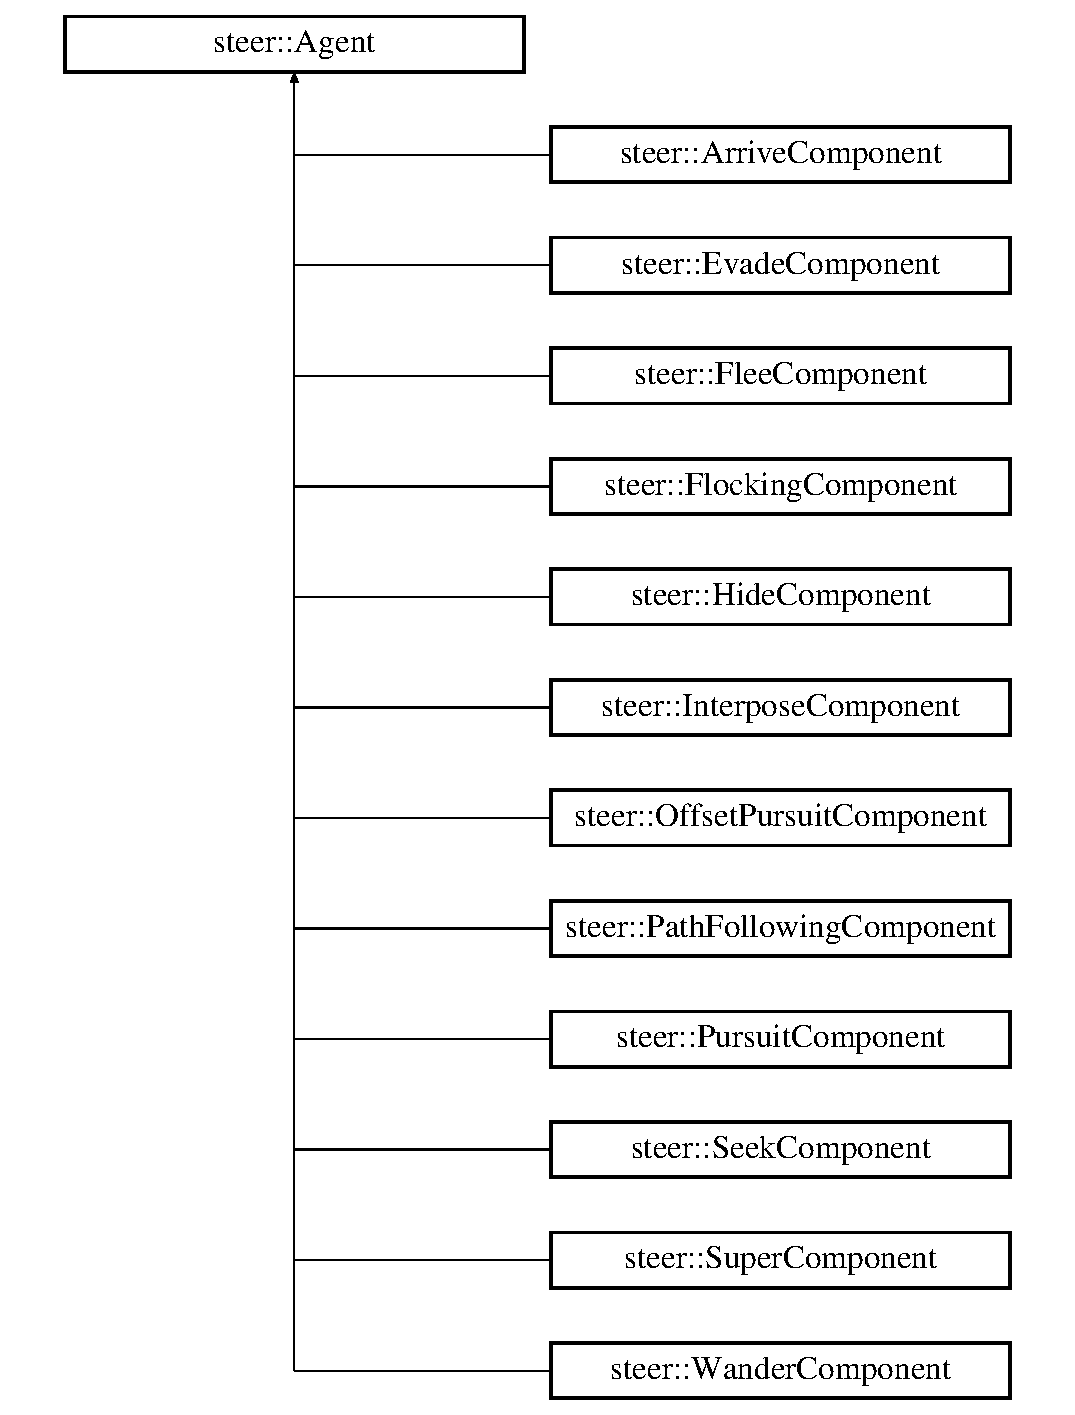
\includegraphics[height=12.000000cm]{classsteer_1_1_agent}
\end{center}
\end{figure}
\subsection*{Public Member Functions}
\begin{DoxyCompactItemize}
\item 
\hypertarget{classsteer_1_1_agent_a681c1d98ec267b9071b66b605f2042d3}{\hyperlink{classsteer_1_1_agent_a681c1d98ec267b9071b66b605f2042d3}{Agent} ()}\label{classsteer_1_1_agent_a681c1d98ec267b9071b66b605f2042d3}

\begin{DoxyCompactList}\small\item\em Default constructor. \end{DoxyCompactList}\item 
\hyperlink{classsteer_1_1_agent_af98ac1281c5f028278d9ab47cf5de03f}{Agent} (\hyperlink{structsteer_1_1_vector2}{steer\-::\-Vector2} position, float radius, \hyperlink{structsteer_1_1_vector2}{steer\-::\-Vector2} velocity, \hyperlink{structsteer_1_1_vector2}{steer\-::\-Vector2} heading, \hyperlink{structsteer_1_1_vector2}{steer\-::\-Vector2} side, float mass, float max\-Speed, float max\-Force, float max\-Turn\-Rate)
\begin{DoxyCompactList}\small\item\em Construct agent from values. \end{DoxyCompactList}\item 
\hyperlink{classsteer_1_1_agent_aadefcfb53b9349ea054718d4d8475e38}{Agent} (\hyperlink{structsteer_1_1_behavior_parameters}{steer\-::\-Behavior\-Parameters} $\ast$params)
\begin{DoxyCompactList}\small\item\em Construct agent from struct of parameters. \end{DoxyCompactList}\item 
\hypertarget{classsteer_1_1_agent_accf89ffc6938e5a62d12cdc69958ff7a}{virtual \hyperlink{classsteer_1_1_agent_accf89ffc6938e5a62d12cdc69958ff7a}{$\sim$\-Agent} ()}\label{classsteer_1_1_agent_accf89ffc6938e5a62d12cdc69958ff7a}

\begin{DoxyCompactList}\small\item\em Destructor. \end{DoxyCompactList}\item 
\hypertarget{classsteer_1_1_agent_acca7800c6bbe61f508c0ccf93fa1850e}{\hyperlink{structsteer_1_1_vector2}{steer\-::\-Vector2} \hyperlink{classsteer_1_1_agent_acca7800c6bbe61f508c0ccf93fa1850e}{get\-Position} () const }\label{classsteer_1_1_agent_acca7800c6bbe61f508c0ccf93fa1850e}

\begin{DoxyCompactList}\small\item\em Gets the position of the entity. \end{DoxyCompactList}\item 
void \hyperlink{classsteer_1_1_agent_a44efb0c0431d55a9785a81d36e0c8fd8}{set\-Position} (\hyperlink{structsteer_1_1_vector2}{steer\-::\-Vector2} new\-Position)
\begin{DoxyCompactList}\small\item\em Sets the position of the entity. \end{DoxyCompactList}\item 
\hypertarget{classsteer_1_1_agent_ad970d8e4e75ea206d230c83ae455d40f}{float \hyperlink{classsteer_1_1_agent_ad970d8e4e75ea206d230c83ae455d40f}{get\-Bounding\-Radius} () const }\label{classsteer_1_1_agent_ad970d8e4e75ea206d230c83ae455d40f}

\begin{DoxyCompactList}\small\item\em Gets the bounding radius of the entity. \end{DoxyCompactList}\item 
void \hyperlink{classsteer_1_1_agent_a7b4578e8f22df3eaa819c8a927fc4a9b}{set\-Bounding\-Radius} (float radius)
\begin{DoxyCompactList}\small\item\em Sets the bounding radius of the entity. \end{DoxyCompactList}\item 
\hypertarget{classsteer_1_1_agent_a3a38a704a0aa83ab080ee429ccced58b}{bool \hyperlink{classsteer_1_1_agent_a3a38a704a0aa83ab080ee429ccced58b}{tagged\-In\-Group} () const }\label{classsteer_1_1_agent_a3a38a704a0aa83ab080ee429ccced58b}

\begin{DoxyCompactList}\small\item\em Gets the tagged status (tagged in a group) of the entity. \end{DoxyCompactList}\item 
\hypertarget{classsteer_1_1_agent_a590e8047a6891d86e404f1639b98bc90}{void \hyperlink{classsteer_1_1_agent_a590e8047a6891d86e404f1639b98bc90}{Tag} ()}\label{classsteer_1_1_agent_a590e8047a6891d86e404f1639b98bc90}

\begin{DoxyCompactList}\small\item\em Tags the entity for an action. \end{DoxyCompactList}\item 
\hypertarget{classsteer_1_1_agent_a44cb0b9e66b3b44b7e9a25471db02a32}{void \hyperlink{classsteer_1_1_agent_a44cb0b9e66b3b44b7e9a25471db02a32}{un\-Tag} ()}\label{classsteer_1_1_agent_a44cb0b9e66b3b44b7e9a25471db02a32}

\begin{DoxyCompactList}\small\item\em Untags the entity. \end{DoxyCompactList}\item 
\hypertarget{classsteer_1_1_agent_aef3484610cf2bcce29965441a0e90edb}{\hyperlink{structsteer_1_1_vector2}{steer\-::\-Vector2} \hyperlink{classsteer_1_1_agent_aef3484610cf2bcce29965441a0e90edb}{get\-Scale} () const }\label{classsteer_1_1_agent_aef3484610cf2bcce29965441a0e90edb}

\begin{DoxyCompactList}\small\item\em Returns the entity's scale. \end{DoxyCompactList}\item 
void \hyperlink{classsteer_1_1_agent_a13bc7f1ce63a393a8de674d209221d17}{set\-Scale} (\hyperlink{structsteer_1_1_vector2}{steer\-::\-Vector2} val)
\begin{DoxyCompactList}\small\item\em Sets the entity's scale from an \hyperlink{structsteer_1_1_vector2}{steer\-::\-Vector2}. \end{DoxyCompactList}\item 
void \hyperlink{classsteer_1_1_agent_ab4203664470868ce7353feaf1d7f2b53}{set\-Scale} (float val)
\begin{DoxyCompactList}\small\item\em Sets the entity's scale from a float. \end{DoxyCompactList}\item 
\hypertarget{classsteer_1_1_agent_adf2555c6a33dbb7b8cf973ecf9abbe6b}{\hyperlink{structsteer_1_1_vector2}{steer\-::\-Vector2} \hyperlink{classsteer_1_1_agent_adf2555c6a33dbb7b8cf973ecf9abbe6b}{get\-Velocity} () const }\label{classsteer_1_1_agent_adf2555c6a33dbb7b8cf973ecf9abbe6b}

\begin{DoxyCompactList}\small\item\em Gets the velocity of the agent. \end{DoxyCompactList}\item 
\hypertarget{classsteer_1_1_agent_a00462a1d6b18521c74de9a4db68b593f}{float \hyperlink{classsteer_1_1_agent_a00462a1d6b18521c74de9a4db68b593f}{get\-Mass} () const }\label{classsteer_1_1_agent_a00462a1d6b18521c74de9a4db68b593f}

\begin{DoxyCompactList}\small\item\em Gets the mass of the agent. Mass is set on construction of the agent only. \end{DoxyCompactList}\item 
\hypertarget{classsteer_1_1_agent_a25da93e8d3da6648e1d6ca00945642a2}{\hyperlink{structsteer_1_1_vector2}{steer\-::\-Vector2} \hyperlink{classsteer_1_1_agent_a25da93e8d3da6648e1d6ca00945642a2}{get\-Side} () const }\label{classsteer_1_1_agent_a25da93e8d3da6648e1d6ca00945642a2}

\begin{DoxyCompactList}\small\item\em Gets the side vector (vector perpendicular to the direction the agent is heading) of the agent. \par
Side is set on construction of the agent only. \end{DoxyCompactList}\item 
void \hyperlink{classsteer_1_1_agent_a4234075d2bb4f6badf69e6eb15241c29}{set\-Side} (const \hyperlink{structsteer_1_1_vector2}{steer\-::\-Vector2} side)
\begin{DoxyCompactList}\small\item\em Sets the side vector (vector perpendicular to the direction the agent is heading) of the agent. \par
Side is set on construction of the agent only. \end{DoxyCompactList}\item 
\hypertarget{classsteer_1_1_agent_a2402cdb0283eae61629524fbcbd5db44}{float \hyperlink{classsteer_1_1_agent_a2402cdb0283eae61629524fbcbd5db44}{get\-Max\-Speed} () const }\label{classsteer_1_1_agent_a2402cdb0283eae61629524fbcbd5db44}

\begin{DoxyCompactList}\small\item\em Gets the max speed of the agent. \end{DoxyCompactList}\item 
void \hyperlink{classsteer_1_1_agent_a992d6071878af809aca1a8e1891d3ed0}{set\-Max\-Speed} (float new\-Speed)
\begin{DoxyCompactList}\small\item\em Sets the velocity of the agent. \end{DoxyCompactList}\item 
\hypertarget{classsteer_1_1_agent_aac77897a0ef9b553971a497019e6c86f}{float \hyperlink{classsteer_1_1_agent_aac77897a0ef9b553971a497019e6c86f}{get\-Max\-Force} () const }\label{classsteer_1_1_agent_aac77897a0ef9b553971a497019e6c86f}

\begin{DoxyCompactList}\small\item\em Gets the max force of the agent. \end{DoxyCompactList}\item 
void \hyperlink{classsteer_1_1_agent_aca5abda307346947bb8d3ac7817882b2}{set\-Max\-Force} (float max\-Force)
\begin{DoxyCompactList}\small\item\em Sets the max force of the agent. \end{DoxyCompactList}\item 
\hypertarget{classsteer_1_1_agent_a6ea6a0aacce16706f3ccc17c233a5a6d}{\hyperlink{structsteer_1_1_vector2}{steer\-::\-Vector2} \hyperlink{classsteer_1_1_agent_a6ea6a0aacce16706f3ccc17c233a5a6d}{get\-Force} () const }\label{classsteer_1_1_agent_a6ea6a0aacce16706f3ccc17c233a5a6d}

\begin{DoxyCompactList}\small\item\em Convenience method, gets the current steering force for the owner agent. Force is public data used for calculating steering force, therefore there is no setter. \end{DoxyCompactList}\item 
\hypertarget{classsteer_1_1_agent_ad78b1ca073d92ed97b035743aa50fe63}{bool \hyperlink{classsteer_1_1_agent_ad78b1ca073d92ed97b035743aa50fe63}{speed\-Maxed\-Out} () const }\label{classsteer_1_1_agent_ad78b1ca073d92ed97b035743aa50fe63}

\begin{DoxyCompactList}\small\item\em Determines if the speed of the agent is maxed out or not. \end{DoxyCompactList}\item 
\hypertarget{classsteer_1_1_agent_a8226ff97ce995f03c7daec808b57edde}{float \hyperlink{classsteer_1_1_agent_a8226ff97ce995f03c7daec808b57edde}{get\-Speed} () const }\label{classsteer_1_1_agent_a8226ff97ce995f03c7daec808b57edde}

\begin{DoxyCompactList}\small\item\em Gets the speed of the agent. \end{DoxyCompactList}\item 
\hypertarget{classsteer_1_1_agent_acf5c7ca1aa5450a3645cbe997d77979f}{float \hyperlink{classsteer_1_1_agent_acf5c7ca1aa5450a3645cbe997d77979f}{get\-Speed\-Squared} () const }\label{classsteer_1_1_agent_acf5c7ca1aa5450a3645cbe997d77979f}

\begin{DoxyCompactList}\small\item\em Gets the speed squared of the agent. \end{DoxyCompactList}\item 
\hypertarget{classsteer_1_1_agent_a3c2fc94062f007f3256b399b7515c67e}{\hyperlink{structsteer_1_1_vector2}{steer\-::\-Vector2} \hyperlink{classsteer_1_1_agent_a3c2fc94062f007f3256b399b7515c67e}{get\-Heading} () const }\label{classsteer_1_1_agent_a3c2fc94062f007f3256b399b7515c67e}

\begin{DoxyCompactList}\small\item\em Gets the heading of the agent. \end{DoxyCompactList}\item 
void \hyperlink{classsteer_1_1_agent_a492dc3524515e1d7890002c606163481}{set\-Heading} (\hyperlink{structsteer_1_1_vector2}{steer\-::\-Vector2} new\-Heading)
\begin{DoxyCompactList}\small\item\em Sets the heading of the agent. \end{DoxyCompactList}\item 
bool \hyperlink{classsteer_1_1_agent_aadf0d39706259827d9273578b4987e18}{rotate\-Heading\-To\-Face\-Position} (\hyperlink{structsteer_1_1_vector2}{steer\-::\-Vector2} target)
\begin{DoxyCompactList}\small\item\em Returns true when the heading is rotated to the target position, returns false otherwise. \end{DoxyCompactList}\item 
\hypertarget{classsteer_1_1_agent_a40fc7801b000897c5f5434ce7d1305a6}{float \hyperlink{classsteer_1_1_agent_a40fc7801b000897c5f5434ce7d1305a6}{get\-Max\-Turn\-Rate} () const }\label{classsteer_1_1_agent_a40fc7801b000897c5f5434ce7d1305a6}

\begin{DoxyCompactList}\small\item\em Gets the max turn rate of the agent. \end{DoxyCompactList}\item 
void \hyperlink{classsteer_1_1_agent_a99de7872a86641efab3a281e2a81fa5a}{set\-Max\-Turn\-Rate} (float max\-Turn\-Rate)
\begin{DoxyCompactList}\small\item\em Sets the max turn rate of the agent. \end{DoxyCompactList}\item 
\hypertarget{classsteer_1_1_agent_a3a96839bccd2e3ba4c828abc0ce98504}{float \hyperlink{classsteer_1_1_agent_a3a96839bccd2e3ba4c828abc0ce98504}{get\-Forward\-Component} ()}\label{classsteer_1_1_agent_a3a96839bccd2e3ba4c828abc0ce98504}

\begin{DoxyCompactList}\small\item\em Calculates the component of the steering force that is parallel with the vehicle heading. \end{DoxyCompactList}\item 
\hypertarget{classsteer_1_1_agent_a8eb6abfe81ef28f6f6ed463b9a0cbb03}{float \hyperlink{classsteer_1_1_agent_a8eb6abfe81ef28f6f6ed463b9a0cbb03}{get\-Side\-Component} ()}\label{classsteer_1_1_agent_a8eb6abfe81ef28f6f6ed463b9a0cbb03}

\begin{DoxyCompactList}\small\item\em Calculates the component of the steering force that is perpendicular with the vehicle heading. \end{DoxyCompactList}\item 
void \hyperlink{classsteer_1_1_agent_abc82085231bd505ef3b00618087fd03a}{set\-Target} (const \hyperlink{structsteer_1_1_vector2}{steer\-::\-Vector2} target)
\begin{DoxyCompactList}\small\item\em Sets the current target for the owner agent. \end{DoxyCompactList}\item 
\hypertarget{classsteer_1_1_agent_adb459be5cce83fece0968c1e12ff09ce}{\hyperlink{structsteer_1_1_vector2}{steer\-::\-Vector2} \hyperlink{classsteer_1_1_agent_adb459be5cce83fece0968c1e12ff09ce}{get\-Target} () const }\label{classsteer_1_1_agent_adb459be5cce83fece0968c1e12ff09ce}

\begin{DoxyCompactList}\small\item\em Gets the current target for the owner agent. \end{DoxyCompactList}\item 
void \hyperlink{classsteer_1_1_agent_ad120d6c1da96904a6425a0a51ad5db3b}{set\-Threat\-Range} (const float range)
\begin{DoxyCompactList}\small\item\em Set the value of the range the object of interest must be in to trigger evasive action. \end{DoxyCompactList}\item 
\hypertarget{classsteer_1_1_agent_a5833ecd792564fde4548e852e7d08663}{float \hyperlink{classsteer_1_1_agent_a5833ecd792564fde4548e852e7d08663}{get\-Threat\-Range} () const }\label{classsteer_1_1_agent_a5833ecd792564fde4548e852e7d08663}

\begin{DoxyCompactList}\small\item\em Get the value of the range the object of interest must be in to trigger evasive action. \end{DoxyCompactList}\item 
void \hyperlink{classsteer_1_1_agent_af7d3e91b9f8367345f04d39b405b6b2d}{set\-Deceleration\-Tweaker} (const float deceleration)
\begin{DoxyCompactList}\small\item\em Set the value for tweaking deceleration for the arrive component. \end{DoxyCompactList}\item 
\hypertarget{classsteer_1_1_agent_ae8f6ad68e363301365de2b32584eabca}{float \hyperlink{classsteer_1_1_agent_ae8f6ad68e363301365de2b32584eabca}{get\-Deceleration\-Tweaker} () const }\label{classsteer_1_1_agent_ae8f6ad68e363301365de2b32584eabca}

\begin{DoxyCompactList}\small\item\em Get the value for tweaking deceleration for the arrive component. \end{DoxyCompactList}\item 
void \hyperlink{classsteer_1_1_agent_a4535a5da819318a0ee8a624c531b1b85}{set\-Wander\-Target} (const \hyperlink{structsteer_1_1_vector2}{steer\-::\-Vector2} target)
\begin{DoxyCompactList}\small\item\em Set the wander target. \end{DoxyCompactList}\item 
\hypertarget{classsteer_1_1_agent_ae09f1e4c1c9bc0db034f8301d826c5d3}{\hyperlink{structsteer_1_1_vector2}{steer\-::\-Vector2} \hyperlink{classsteer_1_1_agent_ae09f1e4c1c9bc0db034f8301d826c5d3}{get\-Wander\-Target} () const }\label{classsteer_1_1_agent_ae09f1e4c1c9bc0db034f8301d826c5d3}

\begin{DoxyCompactList}\small\item\em Get the wander target. \end{DoxyCompactList}\item 
void \hyperlink{classsteer_1_1_agent_adee2526f7be4a3172e1c10f991396ce2}{set\-Wander\-Jitter} (const float jitter)
\begin{DoxyCompactList}\small\item\em Set the wander jitter. \end{DoxyCompactList}\item 
\hypertarget{classsteer_1_1_agent_a05d72edae38d8e73b468af668bbe1d09}{float \hyperlink{classsteer_1_1_agent_a05d72edae38d8e73b468af668bbe1d09}{get\-Wander\-Jitter} () const }\label{classsteer_1_1_agent_a05d72edae38d8e73b468af668bbe1d09}

\begin{DoxyCompactList}\small\item\em Get the wander jitter. \end{DoxyCompactList}\item 
void \hyperlink{classsteer_1_1_agent_a68e2e677a981e66321d85b480e4b9f0f}{set\-Wander\-Radius} (const float radius)
\begin{DoxyCompactList}\small\item\em Set the radius that the agent will wander toward. \end{DoxyCompactList}\item 
\hypertarget{classsteer_1_1_agent_ae2785325858f0d8a933722abb272e517}{float \hyperlink{classsteer_1_1_agent_ae2785325858f0d8a933722abb272e517}{get\-Wander\-Radius} () const }\label{classsteer_1_1_agent_ae2785325858f0d8a933722abb272e517}

\begin{DoxyCompactList}\small\item\em Get the radius the agent is wandering toward. \end{DoxyCompactList}\item 
void \hyperlink{classsteer_1_1_agent_aff41b2f86f61a554d3e2788baff6493b}{set\-Wander\-Distance} (const float distance)
\begin{DoxyCompactList}\small\item\em Set the distance the agent will wander. \end{DoxyCompactList}\item 
\hypertarget{classsteer_1_1_agent_a884eebde33e5cf3919aed101352c0d00}{float \hyperlink{classsteer_1_1_agent_a884eebde33e5cf3919aed101352c0d00}{get\-Wander\-Distance} () const }\label{classsteer_1_1_agent_a884eebde33e5cf3919aed101352c0d00}

\begin{DoxyCompactList}\small\item\em Get the distance the agent will wander. \end{DoxyCompactList}\item 
void \hyperlink{classsteer_1_1_agent_abdadb99a029745ca22ffa5a6d615f295}{set\-Distance\-Buffer} (const float buffer)
\begin{DoxyCompactList}\small\item\em Set the value for the buffer which dictates the minimum distance from a given area (for example, a hiding spot behind an obstacle). \end{DoxyCompactList}\item 
\hypertarget{classsteer_1_1_agent_ab356d904b06ee8a654b8cf0e9512439f}{float \hyperlink{classsteer_1_1_agent_ab356d904b06ee8a654b8cf0e9512439f}{get\-Distance\-Buffer} () const }\label{classsteer_1_1_agent_ab356d904b06ee8a654b8cf0e9512439f}

\begin{DoxyCompactList}\small\item\em Get the value for the distance buffer (minimum distance between self and a given area). \end{DoxyCompactList}\item 
\hypertarget{classsteer_1_1_agent_a1df4096608824947013a135b8215ac26}{void \hyperlink{classsteer_1_1_agent_a1df4096608824947013a135b8215ac26}{set\-Offset} (const \hyperlink{structsteer_1_1_vector2}{steer\-::\-Vector2} offset)}\label{classsteer_1_1_agent_a1df4096608824947013a135b8215ac26}

\begin{DoxyCompactList}\small\item\em Sets the current steering offset for the owner agent -\/ used for tweaking steering force. \end{DoxyCompactList}\item 
\hyperlink{structsteer_1_1_vector2}{steer\-::\-Vector2} \hyperlink{classsteer_1_1_agent_adbe78075e9c9e4bb4dc5355ba68fa3af}{get\-Offset} () const 
\begin{DoxyCompactList}\small\item\em Gets the current steering offset for the owner agent -\/. \end{DoxyCompactList}\item 
\hypertarget{classsteer_1_1_agent_a2270f8a98159dd4fbb8ad30a0e74ef11}{void \hyperlink{classsteer_1_1_agent_a2270f8a98159dd4fbb8ad30a0e74ef11}{create\-Feelers} ()}\label{classsteer_1_1_agent_a2270f8a98159dd4fbb8ad30a0e74ef11}

\begin{DoxyCompactList}\small\item\em A method for creating the feelers used for obstacle and wall avoidance;. \end{DoxyCompactList}\item 
\hypertarget{classsteer_1_1_agent_aef80b80a4bad78fb564d6891e6928a2f}{float \hyperlink{classsteer_1_1_agent_aef80b80a4bad78fb564d6891e6928a2f}{box\-Length} () const }\label{classsteer_1_1_agent_aef80b80a4bad78fb564d6891e6928a2f}

\begin{DoxyCompactList}\small\item\em Returns the value of box length used for obstacle and wall avoidance;. \end{DoxyCompactList}\item 
void \hyperlink{classsteer_1_1_agent_a219803145249f452cb11c566a906214d}{set\-Box\-Length} (const float length)
\begin{DoxyCompactList}\small\item\em Returns the value of box length used for obstacle and wall avoidance;. \end{DoxyCompactList}\item 
\hypertarget{classsteer_1_1_agent_a424e5fc99388933b1da711b5d1308ff4}{const std\-::vector\\*
$<$ \hyperlink{structsteer_1_1_vector2}{steer\-::\-Vector2} $>$ \& \hyperlink{classsteer_1_1_agent_a424e5fc99388933b1da711b5d1308ff4}{get\-Feelers} () const }\label{classsteer_1_1_agent_a424e5fc99388933b1da711b5d1308ff4}

\begin{DoxyCompactList}\small\item\em Returns a reference to the feelers used for obstacle and wall avoidance;. \end{DoxyCompactList}\item 
virtual bool \hyperlink{classsteer_1_1_agent_a707204e49e6519c7a8ea0f3ded608d98}{on} (\hyperlink{namespacesteer_afe6e72f8f8088962727051501181acbe}{steer\-::behavior\-Type} behavior)=0
\begin{DoxyCompactList}\small\item\em This pure virtual function tests if a specific bit of m\-\_\-i\-Flags is set using bitwise operations. Must be overridden in derived classes. \end{DoxyCompactList}\item 
virtual void \hyperlink{classsteer_1_1_agent_ab52d1f7efa08cec0dd516e33551a6a83}{set\-Summing\-Method} (Uint32 sum\-Method)
\begin{DoxyCompactList}\small\item\em A virtual method used for setting the summing method for steering forces. \end{DoxyCompactList}\item 
virtual bool \hyperlink{classsteer_1_1_agent_a00cff0b81bac1d46293d64ce1e3517af}{accumulate\-Force} (\hyperlink{structsteer_1_1_vector2}{steer\-::\-Vector2} \&starting\-Force, \hyperlink{structsteer_1_1_vector2}{steer\-::\-Vector2} force\-To\-Add)
\begin{DoxyCompactList}\small\item\em A virtual method used to accumulate forces from a combination of behaviors. Does nothing, override and implement in derived classes. \end{DoxyCompactList}\item 
\hypertarget{classsteer_1_1_agent_a5d0a4aeb34d48bd120ad68b713a44818}{virtual \hyperlink{structsteer_1_1_vector2}{steer\-::\-Vector2} {\bfseries calculate\-Weighted\-Sum} ()}\label{classsteer_1_1_agent_a5d0a4aeb34d48bd120ad68b713a44818}

\item 
\hypertarget{classsteer_1_1_agent_a127df9a02a6313414adc8aa5ffa83cc3}{virtual \hyperlink{structsteer_1_1_vector2}{steer\-::\-Vector2} {\bfseries calculate\-Prioritized} ()}\label{classsteer_1_1_agent_a127df9a02a6313414adc8aa5ffa83cc3}

\item 
\hypertarget{classsteer_1_1_agent_ac20318e22f798b3b3ec9c18608e8efbf}{virtual \hyperlink{structsteer_1_1_vector2}{steer\-::\-Vector2} \hyperlink{classsteer_1_1_agent_ac20318e22f798b3b3ec9c18608e8efbf}{Calculate} ()=0}\label{classsteer_1_1_agent_ac20318e22f798b3b3ec9c18608e8efbf}

\begin{DoxyCompactList}\small\item\em A pure virtual method for calculating the steering vector. \end{DoxyCompactList}\item 
\hypertarget{classsteer_1_1_agent_a7727670eac2ea8ff53c4101f10198969}{float \hyperlink{classsteer_1_1_agent_a7727670eac2ea8ff53c4101f10198969}{get\-Elapsed\-Time} ()}\label{classsteer_1_1_agent_a7727670eac2ea8ff53c4101f10198969}

\begin{DoxyCompactList}\small\item\em Get the time elapsed since the last frame. \end{DoxyCompactList}\item 
\hypertarget{classsteer_1_1_agent_acb81ecee35acc69f89fdee97f4b6baad}{float \hyperlink{classsteer_1_1_agent_acb81ecee35acc69f89fdee97f4b6baad}{set\-Elapsed\-Time} (float e)}\label{classsteer_1_1_agent_acb81ecee35acc69f89fdee97f4b6baad}

\begin{DoxyCompactList}\small\item\em Set the time elapsed since the last frame. \end{DoxyCompactList}\end{DoxyCompactItemize}
\subsection*{Public Attributes}
\begin{DoxyCompactItemize}
\item 
\hypertarget{classsteer_1_1_agent_a460f141af67ed089ab2c75ea8f710483}{\hyperlink{structsteer_1_1_vector2}{steer\-::\-Vector2} \hyperlink{classsteer_1_1_agent_a460f141af67ed089ab2c75ea8f710483}{m\-\_\-agent\-Position}}\label{classsteer_1_1_agent_a460f141af67ed089ab2c75ea8f710483}

\begin{DoxyCompactList}\small\item\em The Entity's internal position value. \end{DoxyCompactList}\item 
\hypertarget{classsteer_1_1_agent_aee653601201ee2f703c5f0ae9f1e86f0}{\hyperlink{structsteer_1_1_vector2}{steer\-::\-Vector2} \hyperlink{classsteer_1_1_agent_aee653601201ee2f703c5f0ae9f1e86f0}{m\-\_\-scale}}\label{classsteer_1_1_agent_aee653601201ee2f703c5f0ae9f1e86f0}

\begin{DoxyCompactList}\small\item\em The Entity's internal scale value. \end{DoxyCompactList}\item 
\hypertarget{classsteer_1_1_agent_ad6d2ab363bf749ef3ae3289f9044991d}{bool {\bfseries m\-\_\-tag}}\label{classsteer_1_1_agent_ad6d2ab363bf749ef3ae3289f9044991d}

\item 
float \hyperlink{classsteer_1_1_agent_aec01d1d8d1d1e75714ccc41e2a9d2c8f}{m\-\_\-bounding\-Radius}
\begin{DoxyCompactList}\small\item\em Generic flag to indicate that the entity is flagged for some process. \end{DoxyCompactList}\item 
\hypertarget{classsteer_1_1_agent_ab24747403d324e6d3900f4cd07245cef}{\hyperlink{structsteer_1_1_vector2}{steer\-::\-Vector2} \hyperlink{classsteer_1_1_agent_ab24747403d324e6d3900f4cd07245cef}{m\-\_\-steering\-Force}}\label{classsteer_1_1_agent_ab24747403d324e6d3900f4cd07245cef}

\begin{DoxyCompactList}\small\item\em For calculating the steering force internally from all combined behaviors. \end{DoxyCompactList}\item 
\hypertarget{classsteer_1_1_agent_a10a7638abe7f1a5b02663aa2e4d9eab7}{float \hyperlink{classsteer_1_1_agent_a10a7638abe7f1a5b02663aa2e4d9eab7}{m\-\_\-waypoint\-Seek\-Distance\-Squared}}\label{classsteer_1_1_agent_a10a7638abe7f1a5b02663aa2e4d9eab7}

\begin{DoxyCompactList}\small\item\em the distance (squared) a vehicle has to be from a path waypoint before it starts seeking to the next waypoint \end{DoxyCompactList}\item 
\hypertarget{classsteer_1_1_agent_ac7bc35e3b79fa41f74934b5c1f60513d}{std\-::vector$<$ \hyperlink{structsteer_1_1_vector2}{steer\-::\-Vector2} $>$ \hyperlink{classsteer_1_1_agent_ac7bc35e3b79fa41f74934b5c1f60513d}{m\-\_\-feelers}}\label{classsteer_1_1_agent_ac7bc35e3b79fa41f74934b5c1f60513d}

\begin{DoxyCompactList}\small\item\em a vertex buffer to contain the feelers for wall avoidance \end{DoxyCompactList}\item 
\hypertarget{classsteer_1_1_agent_a55b255a2c414feae7685766e559f50d0}{\hyperlink{structsteer_1_1_vector2}{steer\-::\-Vector2} \hyperlink{classsteer_1_1_agent_a55b255a2c414feae7685766e559f50d0}{m\-\_\-velocity}}\label{classsteer_1_1_agent_a55b255a2c414feae7685766e559f50d0}

\begin{DoxyCompactList}\small\item\em Storage for the agent's velocity. \end{DoxyCompactList}\item 
\hypertarget{classsteer_1_1_agent_a671f73d052bea058f989d51848073f8a}{\hyperlink{structsteer_1_1_vector2}{steer\-::\-Vector2} \hyperlink{classsteer_1_1_agent_a671f73d052bea058f989d51848073f8a}{m\-\_\-heading}}\label{classsteer_1_1_agent_a671f73d052bea058f989d51848073f8a}

\begin{DoxyCompactList}\small\item\em Storage for the agent's normalized vector pointing in the direction it is headed. \end{DoxyCompactList}\item 
\hypertarget{classsteer_1_1_agent_a9d823a2a11d22b8f83937d3b22814d97}{\hyperlink{structsteer_1_1_vector2}{steer\-::\-Vector2} \hyperlink{classsteer_1_1_agent_a9d823a2a11d22b8f83937d3b22814d97}{m\-\_\-side}}\label{classsteer_1_1_agent_a9d823a2a11d22b8f83937d3b22814d97}

\begin{DoxyCompactList}\small\item\em A vector perpendicular to the direction the agent is heading. \end{DoxyCompactList}\item 
\hypertarget{classsteer_1_1_agent_a46cd511eacd52f8ba6094160b3670145}{float \hyperlink{classsteer_1_1_agent_a46cd511eacd52f8ba6094160b3670145}{m\-\_\-mass}}\label{classsteer_1_1_agent_a46cd511eacd52f8ba6094160b3670145}

\begin{DoxyCompactList}\small\item\em Mass of the agent. \end{DoxyCompactList}\item 
\hypertarget{classsteer_1_1_agent_aca506229fe40b1fc763d49b34a4c6ef2}{float \hyperlink{classsteer_1_1_agent_aca506229fe40b1fc763d49b34a4c6ef2}{m\-\_\-time\-Elapsed}}\label{classsteer_1_1_agent_aca506229fe40b1fc763d49b34a4c6ef2}

\begin{DoxyCompactList}\small\item\em The time elapsed since the last frame -\/ useful for some steering behavior calcuations. \end{DoxyCompactList}\item 
\hypertarget{classsteer_1_1_agent_a3a3d65b2cc0f85c680c452a894e44172}{\hyperlink{structsteer_1_1_vector2}{steer\-::\-Vector2} \hyperlink{classsteer_1_1_agent_a3a3d65b2cc0f85c680c452a894e44172}{m\-\_\-offset}}\label{classsteer_1_1_agent_a3a3d65b2cc0f85c680c452a894e44172}

\begin{DoxyCompactList}\small\item\em any offset used for formations or offset pursuit \end{DoxyCompactList}\item 
\hypertarget{classsteer_1_1_agent_a265dee803486d6c7d3e70483e45dcbfd}{float \hyperlink{classsteer_1_1_agent_a265dee803486d6c7d3e70483e45dcbfd}{m\-\_\-view\-Distance}}\label{classsteer_1_1_agent_a265dee803486d6c7d3e70483e45dcbfd}

\begin{DoxyCompactList}\small\item\em how far the agent can 'see' \end{DoxyCompactList}\item 
\hypertarget{classsteer_1_1_agent_abf889b7734560a7680a9a866e9ba991d}{Uint32 \hyperlink{classsteer_1_1_agent_abf889b7734560a7680a9a866e9ba991d}{m\-\_\-deceleration}}\label{classsteer_1_1_agent_abf889b7734560a7680a9a866e9ba991d}

\begin{DoxyCompactList}\small\item\em Deceleration type (slow, normal, fast) -\/ S\-E\-E D\-E\-C\-L\-E\-R\-A\-T\-I\-O\-N E\-N\-U\-M in \hyperlink{_behavior_helpers_8hpp_source}{B\-E\-H\-A\-V\-I\-O\-R\-H\-E\-L\-P\-E\-R\-S.\-H\-P\-P}. \end{DoxyCompactList}\item 
\hypertarget{classsteer_1_1_agent_ad2b2a8dc7d465223df5d70d04d0fbae1}{float \hyperlink{classsteer_1_1_agent_ad2b2a8dc7d465223df5d70d04d0fbae1}{m\-\_\-box\-Length}}\label{classsteer_1_1_agent_ad2b2a8dc7d465223df5d70d04d0fbae1}

\begin{DoxyCompactList}\small\item\em length of the 'detection box' utilized in obstacle avoidance \end{DoxyCompactList}\item 
\hypertarget{classsteer_1_1_agent_a4829d7657898902c398ab200ab07b020}{float \hyperlink{classsteer_1_1_agent_a4829d7657898902c398ab200ab07b020}{m\-\_\-wall\-Detection\-Feeler\-Length}}\label{classsteer_1_1_agent_a4829d7657898902c398ab200ab07b020}

\begin{DoxyCompactList}\small\item\em the length of the 'feeler/s' used in wall detection \end{DoxyCompactList}\item 
\hypertarget{classsteer_1_1_agent_aba01853b986d8386b82dc5cf4277237d}{float \hyperlink{classsteer_1_1_agent_aba01853b986d8386b82dc5cf4277237d}{m\-\_\-max\-Speed}}\label{classsteer_1_1_agent_aba01853b986d8386b82dc5cf4277237d}

\begin{DoxyCompactList}\small\item\em The maximum speed at which the agent can travel. \end{DoxyCompactList}\item 
\hypertarget{classsteer_1_1_agent_a907901caead6a63c29189ce837353603}{float \hyperlink{classsteer_1_1_agent_a907901caead6a63c29189ce837353603}{m\-\_\-max\-Force}}\label{classsteer_1_1_agent_a907901caead6a63c29189ce837353603}

\begin{DoxyCompactList}\small\item\em The maximum force the agent can use to propel itself. \end{DoxyCompactList}\item 
\hypertarget{classsteer_1_1_agent_a89547020b0796ffc7c184346788bab6d}{float \hyperlink{classsteer_1_1_agent_a89547020b0796ffc7c184346788bab6d}{m\-\_\-max\-Turn\-Rate}}\label{classsteer_1_1_agent_a89547020b0796ffc7c184346788bab6d}

\begin{DoxyCompactList}\small\item\em The maximum rate at which the agent can rotate. \end{DoxyCompactList}\item 
\hypertarget{classsteer_1_1_agent_a705eef01aa4f585256e185e140c2b032}{\hyperlink{structsteer_1_1_vector2}{steer\-::\-Vector2} \hyperlink{classsteer_1_1_agent_a705eef01aa4f585256e185e140c2b032}{m\-\_\-target}}\label{classsteer_1_1_agent_a705eef01aa4f585256e185e140c2b032}

\begin{DoxyCompactList}\small\item\em For setting the agent's target. \end{DoxyCompactList}\item 
\hypertarget{classsteer_1_1_agent_a21c017c11309bec6e38e76361f630455}{float \hyperlink{classsteer_1_1_agent_a21c017c11309bec6e38e76361f630455}{m\-\_\-threat\-Range}}\label{classsteer_1_1_agent_a21c017c11309bec6e38e76361f630455}

\begin{DoxyCompactList}\small\item\em Range the object of interest must be in to trigger evasive action. \end{DoxyCompactList}\item 
\hypertarget{classsteer_1_1_agent_ab600b61ca90b8f0bc1af498e5654d098}{float \hyperlink{classsteer_1_1_agent_ab600b61ca90b8f0bc1af498e5654d098}{m\-\_\-deceleration\-Tweaker}}\label{classsteer_1_1_agent_ab600b61ca90b8f0bc1af498e5654d098}

\begin{DoxyCompactList}\small\item\em Value used to tweak deceleration. \end{DoxyCompactList}\item 
\hypertarget{classsteer_1_1_agent_a8beb6a135392910d5e55339c7746263d}{float \hyperlink{classsteer_1_1_agent_a8beb6a135392910d5e55339c7746263d}{m\-\_\-distance\-Buffer}}\label{classsteer_1_1_agent_a8beb6a135392910d5e55339c7746263d}

\begin{DoxyCompactList}\small\item\em Value used to set the distance buffer. \end{DoxyCompactList}\item 
\hypertarget{classsteer_1_1_agent_afa1c07fbea2b54bf3a404153a0cd61c0}{\hyperlink{structsteer_1_1_vector2}{steer\-::\-Vector2} \hyperlink{classsteer_1_1_agent_afa1c07fbea2b54bf3a404153a0cd61c0}{m\-\_\-wander\-Target}}\label{classsteer_1_1_agent_afa1c07fbea2b54bf3a404153a0cd61c0}

\begin{DoxyCompactList}\small\item\em the current position on the wander circle the agent is attempting to steer towards \end{DoxyCompactList}\item 
\hypertarget{classsteer_1_1_agent_abccf322de46725b1c42ee92673397067}{float \hyperlink{classsteer_1_1_agent_abccf322de46725b1c42ee92673397067}{m\-\_\-wander\-Jitter}}\label{classsteer_1_1_agent_abccf322de46725b1c42ee92673397067}

\begin{DoxyCompactList}\small\item\em Amount of displacement along the constraining circle for the wandering agent. \end{DoxyCompactList}\item 
\hypertarget{classsteer_1_1_agent_af3adf53b47e918c4deb1196e2125a9c5}{float \hyperlink{classsteer_1_1_agent_af3adf53b47e918c4deb1196e2125a9c5}{m\-\_\-wander\-Radius}}\label{classsteer_1_1_agent_af3adf53b47e918c4deb1196e2125a9c5}

\begin{DoxyCompactList}\small\item\em The radius of the constraining circle for the wandering agent. \end{DoxyCompactList}\item 
\hypertarget{classsteer_1_1_agent_a211c770227c7eb9485eec1b10d03cddd}{float \hyperlink{classsteer_1_1_agent_a211c770227c7eb9485eec1b10d03cddd}{m\-\_\-wander\-Distance}}\label{classsteer_1_1_agent_a211c770227c7eb9485eec1b10d03cddd}

\begin{DoxyCompactList}\small\item\em Distance the wander circle is projected in front of the agent. \end{DoxyCompactList}\end{DoxyCompactItemize}


\subsection{Detailed Description}
The invisible, but highly necessary, automaton which drives your $\ast$game entity/graphical representation's motion. Getters and Setters are provided, $\ast$however it will always be easier to just use the data -\/ since it is all public. 

\subsection{Constructor \& Destructor Documentation}
\hypertarget{classsteer_1_1_agent_af98ac1281c5f028278d9ab47cf5de03f}{\index{steer\-::\-Agent@{steer\-::\-Agent}!Agent@{Agent}}
\index{Agent@{Agent}!steer::Agent@{steer\-::\-Agent}}
\subsubsection[{Agent}]{\setlength{\rightskip}{0pt plus 5cm}steer\-::\-Agent\-::\-Agent (
\begin{DoxyParamCaption}
\item[{{\bf steer\-::\-Vector2}}]{position, }
\item[{float}]{radius, }
\item[{{\bf steer\-::\-Vector2}}]{velocity, }
\item[{{\bf steer\-::\-Vector2}}]{heading, }
\item[{{\bf steer\-::\-Vector2}}]{side, }
\item[{float}]{mass, }
\item[{float}]{max\-Speed, }
\item[{float}]{max\-Force, }
\item[{float}]{max\-Turn\-Rate}
\end{DoxyParamCaption}
)}}\label{classsteer_1_1_agent_af98ac1281c5f028278d9ab47cf5de03f}


Construct agent from values. 


\begin{DoxyParams}{Parameters}
{\em position} & -\/ a \hyperlink{structsteer_1_1_vector2}{steer\-::\-Vector2} of floats. \\
\hline
{\em radius} & -\/ a plain old float. \\
\hline
{\em velocity} & -\/ a \hyperlink{structsteer_1_1_vector2}{steer\-::\-Vector2} of floats. \\
\hline
{\em heading} & -\/ a \hyperlink{structsteer_1_1_vector2}{steer\-::\-Vector2} of floats. \\
\hline
{\em side} & -\/ a \hyperlink{structsteer_1_1_vector2}{steer\-::\-Vector2} of floats. \\
\hline
{\em mass} & -\/ a plain old float. \\
\hline
{\em max\-Speed} & -\/ a plain old float. \\
\hline
{\em max\-Force} & -\/ a plain old float. \\
\hline
{\em max\-Turn\-Rate} & -\/ a plain old float. \\
\hline
\end{DoxyParams}
\hypertarget{classsteer_1_1_agent_aadefcfb53b9349ea054718d4d8475e38}{\index{steer\-::\-Agent@{steer\-::\-Agent}!Agent@{Agent}}
\index{Agent@{Agent}!steer::Agent@{steer\-::\-Agent}}
\subsubsection[{Agent}]{\setlength{\rightskip}{0pt plus 5cm}steer\-::\-Agent\-::\-Agent (
\begin{DoxyParamCaption}
\item[{{\bf steer\-::\-Behavior\-Parameters} $\ast$}]{params}
\end{DoxyParamCaption}
)}}\label{classsteer_1_1_agent_aadefcfb53b9349ea054718d4d8475e38}


Construct agent from struct of parameters. 


\begin{DoxyParams}{Parameters}
{\em params} & -\/ a \hyperlink{structsteer_1_1_behavior_parameters}{steer\-::\-Behavior\-Parameters} object; \\
\hline
\end{DoxyParams}


\subsection{Member Function Documentation}
\hypertarget{classsteer_1_1_agent_a00cff0b81bac1d46293d64ce1e3517af}{\index{steer\-::\-Agent@{steer\-::\-Agent}!accumulate\-Force@{accumulate\-Force}}
\index{accumulate\-Force@{accumulate\-Force}!steer::Agent@{steer\-::\-Agent}}
\subsubsection[{accumulate\-Force}]{\setlength{\rightskip}{0pt plus 5cm}bool steer\-::\-Agent\-::accumulate\-Force (
\begin{DoxyParamCaption}
\item[{{\bf steer\-::\-Vector2} \&}]{starting\-Force, }
\item[{{\bf steer\-::\-Vector2}}]{force\-To\-Add}
\end{DoxyParamCaption}
)\hspace{0.3cm}{\ttfamily [virtual]}}}\label{classsteer_1_1_agent_a00cff0b81bac1d46293d64ce1e3517af}


A virtual method used to accumulate forces from a combination of behaviors. Does nothing, override and implement in derived classes. 


\begin{DoxyParams}{Parameters}
{\em starting\-Force} & -\/ a \hyperlink{structsteer_1_1_vector2}{steer\-::\-Vector2} of floats. \\
\hline
{\em force\-To\-Add} & -\/ a \hyperlink{structsteer_1_1_vector2}{steer\-::\-Vector2} of floats. \\
\hline
\end{DoxyParams}
\hypertarget{classsteer_1_1_agent_adbe78075e9c9e4bb4dc5355ba68fa3af}{\index{steer\-::\-Agent@{steer\-::\-Agent}!get\-Offset@{get\-Offset}}
\index{get\-Offset@{get\-Offset}!steer::Agent@{steer\-::\-Agent}}
\subsubsection[{get\-Offset}]{\setlength{\rightskip}{0pt plus 5cm}{\bf steer\-::\-Vector2} steer\-::\-Agent\-::get\-Offset (
\begin{DoxyParamCaption}
{}
\end{DoxyParamCaption}
) const\hspace{0.3cm}{\ttfamily [inline]}}}\label{classsteer_1_1_agent_adbe78075e9c9e4bb4dc5355ba68fa3af}


Gets the current steering offset for the owner agent -\/. 

\begin{DoxySeeAlso}{See Also}
\hyperlink{classsteer_1_1_agent_a1df4096608824947013a135b8215ac26}{set\-Offset(const steer\-::\-Vector2 offset)}; 
\end{DoxySeeAlso}
\hypertarget{classsteer_1_1_agent_a707204e49e6519c7a8ea0f3ded608d98}{\index{steer\-::\-Agent@{steer\-::\-Agent}!on@{on}}
\index{on@{on}!steer::Agent@{steer\-::\-Agent}}
\subsubsection[{on}]{\setlength{\rightskip}{0pt plus 5cm}bool steer\-::\-Agent\-::on (
\begin{DoxyParamCaption}
\item[{{\bf steer\-::behavior\-Type}}]{behavior}
\end{DoxyParamCaption}
)\hspace{0.3cm}{\ttfamily [pure virtual]}}}\label{classsteer_1_1_agent_a707204e49e6519c7a8ea0f3ded608d98}


This pure virtual function tests if a specific bit of m\-\_\-i\-Flags is set using bitwise operations. Must be overridden in derived classes. 


\begin{DoxyParams}{Parameters}
{\em behavior} & -\/ enum behavior\-Type. \\
\hline
\end{DoxyParams}


Implemented in \hyperlink{classsteer_1_1_hide_component_a64ff14630f96232381dd0fd88c1d9d04}{steer\-::\-Hide\-Component}, \hyperlink{classsteer_1_1_path_following_component_af15d403db80ac9d623d6fc4ec6f6701b}{steer\-::\-Path\-Following\-Component}, \hyperlink{classsteer_1_1_arrive_component_ac904acaeee6865089e3255cf8d7390ce}{steer\-::\-Arrive\-Component}, \hyperlink{classsteer_1_1_evade_component_a7e71d5e7024ed7bce4624c831477f67b}{steer\-::\-Evade\-Component}, \hyperlink{classsteer_1_1_flee_component_a7e344d7ea6b5b2f3e50ef7f21ec1ab10}{steer\-::\-Flee\-Component}, \hyperlink{classsteer_1_1_wander_component_abf53f90d185d86aebf2cb744fac59f37}{steer\-::\-Wander\-Component}, \hyperlink{classsteer_1_1_interpose_component_a0ad5f9af346843c67983d103d1e3d167}{steer\-::\-Interpose\-Component}, \hyperlink{classsteer_1_1_offset_pursuit_component_a748847de5cec80589b12b35214c5b5e2}{steer\-::\-Offset\-Pursuit\-Component}, \hyperlink{classsteer_1_1_pursuit_component_a10e4d08aaca8aaf3d7041e281af2a519}{steer\-::\-Pursuit\-Component}, \hyperlink{classsteer_1_1_seek_component_a02782af7638a7dfc59de647ba810d0ae}{steer\-::\-Seek\-Component}, \hyperlink{classsteer_1_1_flocking_component_a0d788eaec845b83503a7918e984cfd5b}{steer\-::\-Flocking\-Component}, and \hyperlink{classsteer_1_1_super_component_a6d4b33b6f838d89216e11d8f2a427f58}{steer\-::\-Super\-Component}.

\hypertarget{classsteer_1_1_agent_aadf0d39706259827d9273578b4987e18}{\index{steer\-::\-Agent@{steer\-::\-Agent}!rotate\-Heading\-To\-Face\-Position@{rotate\-Heading\-To\-Face\-Position}}
\index{rotate\-Heading\-To\-Face\-Position@{rotate\-Heading\-To\-Face\-Position}!steer::Agent@{steer\-::\-Agent}}
\subsubsection[{rotate\-Heading\-To\-Face\-Position}]{\setlength{\rightskip}{0pt plus 5cm}bool steer\-::\-Agent\-::rotate\-Heading\-To\-Face\-Position (
\begin{DoxyParamCaption}
\item[{{\bf steer\-::\-Vector2}}]{target}
\end{DoxyParamCaption}
)}}\label{classsteer_1_1_agent_aadf0d39706259827d9273578b4987e18}


Returns true when the heading is rotated to the target position, returns false otherwise. 


\begin{DoxyParams}{Parameters}
{\em target} & -\/ a \hyperlink{structsteer_1_1_vector2}{steer\-::\-Vector2} of floats. \\
\hline
\end{DoxyParams}
\hypertarget{classsteer_1_1_agent_a7b4578e8f22df3eaa819c8a927fc4a9b}{\index{steer\-::\-Agent@{steer\-::\-Agent}!set\-Bounding\-Radius@{set\-Bounding\-Radius}}
\index{set\-Bounding\-Radius@{set\-Bounding\-Radius}!steer::Agent@{steer\-::\-Agent}}
\subsubsection[{set\-Bounding\-Radius}]{\setlength{\rightskip}{0pt plus 5cm}void steer\-::\-Agent\-::set\-Bounding\-Radius (
\begin{DoxyParamCaption}
\item[{float}]{radius}
\end{DoxyParamCaption}
)\hspace{0.3cm}{\ttfamily [inline]}}}\label{classsteer_1_1_agent_a7b4578e8f22df3eaa819c8a927fc4a9b}


Sets the bounding radius of the entity. 


\begin{DoxyParams}{Parameters}
{\em radius} & -\/ a plain old float. \\
\hline
\end{DoxyParams}
\hypertarget{classsteer_1_1_agent_a219803145249f452cb11c566a906214d}{\index{steer\-::\-Agent@{steer\-::\-Agent}!set\-Box\-Length@{set\-Box\-Length}}
\index{set\-Box\-Length@{set\-Box\-Length}!steer::Agent@{steer\-::\-Agent}}
\subsubsection[{set\-Box\-Length}]{\setlength{\rightskip}{0pt plus 5cm}void steer\-::\-Agent\-::set\-Box\-Length (
\begin{DoxyParamCaption}
\item[{const float}]{length}
\end{DoxyParamCaption}
)\hspace{0.3cm}{\ttfamily [inline]}}}\label{classsteer_1_1_agent_a219803145249f452cb11c566a906214d}


Returns the value of box length used for obstacle and wall avoidance;. 


\begin{DoxyParams}{Parameters}
{\em length} & -\/ a plain old float. \\
\hline
\end{DoxyParams}
\hypertarget{classsteer_1_1_agent_af7d3e91b9f8367345f04d39b405b6b2d}{\index{steer\-::\-Agent@{steer\-::\-Agent}!set\-Deceleration\-Tweaker@{set\-Deceleration\-Tweaker}}
\index{set\-Deceleration\-Tweaker@{set\-Deceleration\-Tweaker}!steer::Agent@{steer\-::\-Agent}}
\subsubsection[{set\-Deceleration\-Tweaker}]{\setlength{\rightskip}{0pt plus 5cm}void steer\-::\-Agent\-::set\-Deceleration\-Tweaker (
\begin{DoxyParamCaption}
\item[{const float}]{deceleration}
\end{DoxyParamCaption}
)\hspace{0.3cm}{\ttfamily [inline]}}}\label{classsteer_1_1_agent_af7d3e91b9f8367345f04d39b405b6b2d}


Set the value for tweaking deceleration for the arrive component. 


\begin{DoxyParams}{Parameters}
{\em weight} & -\/ a plain old float. \\
\hline
\end{DoxyParams}
\hypertarget{classsteer_1_1_agent_abdadb99a029745ca22ffa5a6d615f295}{\index{steer\-::\-Agent@{steer\-::\-Agent}!set\-Distance\-Buffer@{set\-Distance\-Buffer}}
\index{set\-Distance\-Buffer@{set\-Distance\-Buffer}!steer::Agent@{steer\-::\-Agent}}
\subsubsection[{set\-Distance\-Buffer}]{\setlength{\rightskip}{0pt plus 5cm}void steer\-::\-Agent\-::set\-Distance\-Buffer (
\begin{DoxyParamCaption}
\item[{const float}]{buffer}
\end{DoxyParamCaption}
)\hspace{0.3cm}{\ttfamily [inline]}}}\label{classsteer_1_1_agent_abdadb99a029745ca22ffa5a6d615f295}


Set the value for the buffer which dictates the minimum distance from a given area (for example, a hiding spot behind an obstacle). 


\begin{DoxyParams}{Parameters}
{\em buffer} & -\/ a plain old float. \\
\hline
\end{DoxyParams}
\hypertarget{classsteer_1_1_agent_a492dc3524515e1d7890002c606163481}{\index{steer\-::\-Agent@{steer\-::\-Agent}!set\-Heading@{set\-Heading}}
\index{set\-Heading@{set\-Heading}!steer::Agent@{steer\-::\-Agent}}
\subsubsection[{set\-Heading}]{\setlength{\rightskip}{0pt plus 5cm}void steer\-::\-Agent\-::set\-Heading (
\begin{DoxyParamCaption}
\item[{{\bf steer\-::\-Vector2}}]{new\-Heading}
\end{DoxyParamCaption}
)}}\label{classsteer_1_1_agent_a492dc3524515e1d7890002c606163481}


Sets the heading of the agent. 


\begin{DoxyParams}{Parameters}
{\em new\-Heading} & -\/ a \hyperlink{structsteer_1_1_vector2}{steer\-::\-Vector2} of floats. \\
\hline
\end{DoxyParams}
\hypertarget{classsteer_1_1_agent_aca5abda307346947bb8d3ac7817882b2}{\index{steer\-::\-Agent@{steer\-::\-Agent}!set\-Max\-Force@{set\-Max\-Force}}
\index{set\-Max\-Force@{set\-Max\-Force}!steer::Agent@{steer\-::\-Agent}}
\subsubsection[{set\-Max\-Force}]{\setlength{\rightskip}{0pt plus 5cm}void steer\-::\-Agent\-::set\-Max\-Force (
\begin{DoxyParamCaption}
\item[{float}]{max\-Force}
\end{DoxyParamCaption}
)\hspace{0.3cm}{\ttfamily [inline]}}}\label{classsteer_1_1_agent_aca5abda307346947bb8d3ac7817882b2}


Sets the max force of the agent. 


\begin{DoxyParams}{Parameters}
{\em max\-Force} & -\/ a plain old float. \\
\hline
\end{DoxyParams}
\hypertarget{classsteer_1_1_agent_a992d6071878af809aca1a8e1891d3ed0}{\index{steer\-::\-Agent@{steer\-::\-Agent}!set\-Max\-Speed@{set\-Max\-Speed}}
\index{set\-Max\-Speed@{set\-Max\-Speed}!steer::Agent@{steer\-::\-Agent}}
\subsubsection[{set\-Max\-Speed}]{\setlength{\rightskip}{0pt plus 5cm}void steer\-::\-Agent\-::set\-Max\-Speed (
\begin{DoxyParamCaption}
\item[{float}]{new\-Speed}
\end{DoxyParamCaption}
)\hspace{0.3cm}{\ttfamily [inline]}}}\label{classsteer_1_1_agent_a992d6071878af809aca1a8e1891d3ed0}


Sets the velocity of the agent. 


\begin{DoxyParams}{Parameters}
{\em new\-Speed} & -\/ a plain old float. \\
\hline
\end{DoxyParams}
\hypertarget{classsteer_1_1_agent_a99de7872a86641efab3a281e2a81fa5a}{\index{steer\-::\-Agent@{steer\-::\-Agent}!set\-Max\-Turn\-Rate@{set\-Max\-Turn\-Rate}}
\index{set\-Max\-Turn\-Rate@{set\-Max\-Turn\-Rate}!steer::Agent@{steer\-::\-Agent}}
\subsubsection[{set\-Max\-Turn\-Rate}]{\setlength{\rightskip}{0pt plus 5cm}void steer\-::\-Agent\-::set\-Max\-Turn\-Rate (
\begin{DoxyParamCaption}
\item[{float}]{val}
\end{DoxyParamCaption}
)\hspace{0.3cm}{\ttfamily [inline]}}}\label{classsteer_1_1_agent_a99de7872a86641efab3a281e2a81fa5a}


Sets the max turn rate of the agent. 


\begin{DoxyParams}{Parameters}
{\em max\-Turn\-Rate} & -\/ a plain old float. \\
\hline
\end{DoxyParams}
\hypertarget{classsteer_1_1_agent_a44efb0c0431d55a9785a81d36e0c8fd8}{\index{steer\-::\-Agent@{steer\-::\-Agent}!set\-Position@{set\-Position}}
\index{set\-Position@{set\-Position}!steer::Agent@{steer\-::\-Agent}}
\subsubsection[{set\-Position}]{\setlength{\rightskip}{0pt plus 5cm}void steer\-::\-Agent\-::set\-Position (
\begin{DoxyParamCaption}
\item[{{\bf steer\-::\-Vector2}}]{new\-Position}
\end{DoxyParamCaption}
)\hspace{0.3cm}{\ttfamily [inline]}}}\label{classsteer_1_1_agent_a44efb0c0431d55a9785a81d36e0c8fd8}


Sets the position of the entity. 


\begin{DoxyParams}{Parameters}
{\em new\-Position} & -\/ a \hyperlink{structsteer_1_1_vector2}{steer\-::\-Vector2} of floats. \\
\hline
\end{DoxyParams}
\hypertarget{classsteer_1_1_agent_a13bc7f1ce63a393a8de674d209221d17}{\index{steer\-::\-Agent@{steer\-::\-Agent}!set\-Scale@{set\-Scale}}
\index{set\-Scale@{set\-Scale}!steer::Agent@{steer\-::\-Agent}}
\subsubsection[{set\-Scale}]{\setlength{\rightskip}{0pt plus 5cm}void steer\-::\-Agent\-::set\-Scale (
\begin{DoxyParamCaption}
\item[{{\bf steer\-::\-Vector2}}]{val}
\end{DoxyParamCaption}
)\hspace{0.3cm}{\ttfamily [inline]}}}\label{classsteer_1_1_agent_a13bc7f1ce63a393a8de674d209221d17}


Sets the entity's scale from an \hyperlink{structsteer_1_1_vector2}{steer\-::\-Vector2}. 


\begin{DoxyParams}{Parameters}
{\em val} & -\/ a \hyperlink{structsteer_1_1_vector2}{steer\-::\-Vector2} of floats. \\
\hline
\end{DoxyParams}
\hypertarget{classsteer_1_1_agent_ab4203664470868ce7353feaf1d7f2b53}{\index{steer\-::\-Agent@{steer\-::\-Agent}!set\-Scale@{set\-Scale}}
\index{set\-Scale@{set\-Scale}!steer::Agent@{steer\-::\-Agent}}
\subsubsection[{set\-Scale}]{\setlength{\rightskip}{0pt plus 5cm}void steer\-::\-Agent\-::set\-Scale (
\begin{DoxyParamCaption}
\item[{float}]{val}
\end{DoxyParamCaption}
)\hspace{0.3cm}{\ttfamily [inline]}}}\label{classsteer_1_1_agent_ab4203664470868ce7353feaf1d7f2b53}


Sets the entity's scale from a float. 


\begin{DoxyParams}{Parameters}
{\em val} & -\/ a plain old float. \\
\hline
\end{DoxyParams}
\hypertarget{classsteer_1_1_agent_a4234075d2bb4f6badf69e6eb15241c29}{\index{steer\-::\-Agent@{steer\-::\-Agent}!set\-Side@{set\-Side}}
\index{set\-Side@{set\-Side}!steer::Agent@{steer\-::\-Agent}}
\subsubsection[{set\-Side}]{\setlength{\rightskip}{0pt plus 5cm}void steer\-::\-Agent\-::set\-Side (
\begin{DoxyParamCaption}
\item[{const {\bf steer\-::\-Vector2}}]{side}
\end{DoxyParamCaption}
)\hspace{0.3cm}{\ttfamily [inline]}}}\label{classsteer_1_1_agent_a4234075d2bb4f6badf69e6eb15241c29}


Sets the side vector (vector perpendicular to the direction the agent is heading) of the agent. \par
Side is set on construction of the agent only. 


\begin{DoxyParams}{Parameters}
{\em side} & -\/ a \hyperlink{structsteer_1_1_vector2}{steer\-::\-Vector2} of floats. \\
\hline
\end{DoxyParams}
\hypertarget{classsteer_1_1_agent_ab52d1f7efa08cec0dd516e33551a6a83}{\index{steer\-::\-Agent@{steer\-::\-Agent}!set\-Summing\-Method@{set\-Summing\-Method}}
\index{set\-Summing\-Method@{set\-Summing\-Method}!steer::Agent@{steer\-::\-Agent}}
\subsubsection[{set\-Summing\-Method}]{\setlength{\rightskip}{0pt plus 5cm}void steer\-::\-Agent\-::set\-Summing\-Method (
\begin{DoxyParamCaption}
\item[{Uint32}]{sum\-Method}
\end{DoxyParamCaption}
)\hspace{0.3cm}{\ttfamily [virtual]}}}\label{classsteer_1_1_agent_ab52d1f7efa08cec0dd516e33551a6a83}


A virtual method used for setting the summing method for steering forces. 


\begin{DoxyParams}{Parameters}
{\em sum\-Method} & -\/ an Uint32. \\
\hline
\end{DoxyParams}
\hypertarget{classsteer_1_1_agent_abc82085231bd505ef3b00618087fd03a}{\index{steer\-::\-Agent@{steer\-::\-Agent}!set\-Target@{set\-Target}}
\index{set\-Target@{set\-Target}!steer::Agent@{steer\-::\-Agent}}
\subsubsection[{set\-Target}]{\setlength{\rightskip}{0pt plus 5cm}void steer\-::\-Agent\-::set\-Target (
\begin{DoxyParamCaption}
\item[{const {\bf steer\-::\-Vector2}}]{target}
\end{DoxyParamCaption}
)\hspace{0.3cm}{\ttfamily [inline]}}}\label{classsteer_1_1_agent_abc82085231bd505ef3b00618087fd03a}


Sets the current target for the owner agent. 


\begin{DoxyParams}{Parameters}
{\em target} & -\/ a \hyperlink{structsteer_1_1_vector2}{steer\-::\-Vector2} of floats. \\
\hline
\end{DoxyParams}
\hypertarget{classsteer_1_1_agent_ad120d6c1da96904a6425a0a51ad5db3b}{\index{steer\-::\-Agent@{steer\-::\-Agent}!set\-Threat\-Range@{set\-Threat\-Range}}
\index{set\-Threat\-Range@{set\-Threat\-Range}!steer::Agent@{steer\-::\-Agent}}
\subsubsection[{set\-Threat\-Range}]{\setlength{\rightskip}{0pt plus 5cm}void steer\-::\-Agent\-::set\-Threat\-Range (
\begin{DoxyParamCaption}
\item[{const float}]{range}
\end{DoxyParamCaption}
)\hspace{0.3cm}{\ttfamily [inline]}}}\label{classsteer_1_1_agent_ad120d6c1da96904a6425a0a51ad5db3b}


Set the value of the range the object of interest must be in to trigger evasive action. 


\begin{DoxyParams}{Parameters}
{\em range} & -\/ a plain old float. \\
\hline
\end{DoxyParams}
\hypertarget{classsteer_1_1_agent_aff41b2f86f61a554d3e2788baff6493b}{\index{steer\-::\-Agent@{steer\-::\-Agent}!set\-Wander\-Distance@{set\-Wander\-Distance}}
\index{set\-Wander\-Distance@{set\-Wander\-Distance}!steer::Agent@{steer\-::\-Agent}}
\subsubsection[{set\-Wander\-Distance}]{\setlength{\rightskip}{0pt plus 5cm}void steer\-::\-Agent\-::set\-Wander\-Distance (
\begin{DoxyParamCaption}
\item[{const float}]{distance}
\end{DoxyParamCaption}
)\hspace{0.3cm}{\ttfamily [inline]}}}\label{classsteer_1_1_agent_aff41b2f86f61a554d3e2788baff6493b}


Set the distance the agent will wander. 


\begin{DoxyParams}{Parameters}
{\em distance} & -\/ a plain old float. \\
\hline
\end{DoxyParams}
\hypertarget{classsteer_1_1_agent_adee2526f7be4a3172e1c10f991396ce2}{\index{steer\-::\-Agent@{steer\-::\-Agent}!set\-Wander\-Jitter@{set\-Wander\-Jitter}}
\index{set\-Wander\-Jitter@{set\-Wander\-Jitter}!steer::Agent@{steer\-::\-Agent}}
\subsubsection[{set\-Wander\-Jitter}]{\setlength{\rightskip}{0pt plus 5cm}void steer\-::\-Agent\-::set\-Wander\-Jitter (
\begin{DoxyParamCaption}
\item[{const float}]{jitter}
\end{DoxyParamCaption}
)\hspace{0.3cm}{\ttfamily [inline]}}}\label{classsteer_1_1_agent_adee2526f7be4a3172e1c10f991396ce2}


Set the wander jitter. 


\begin{DoxyParams}{Parameters}
{\em jitter} & -\/ a plain old float. \\
\hline
\end{DoxyParams}
\hypertarget{classsteer_1_1_agent_a68e2e677a981e66321d85b480e4b9f0f}{\index{steer\-::\-Agent@{steer\-::\-Agent}!set\-Wander\-Radius@{set\-Wander\-Radius}}
\index{set\-Wander\-Radius@{set\-Wander\-Radius}!steer::Agent@{steer\-::\-Agent}}
\subsubsection[{set\-Wander\-Radius}]{\setlength{\rightskip}{0pt plus 5cm}void steer\-::\-Agent\-::set\-Wander\-Radius (
\begin{DoxyParamCaption}
\item[{const float}]{radius}
\end{DoxyParamCaption}
)\hspace{0.3cm}{\ttfamily [inline]}}}\label{classsteer_1_1_agent_a68e2e677a981e66321d85b480e4b9f0f}


Set the radius that the agent will wander toward. 


\begin{DoxyParams}{Parameters}
{\em radius} & -\/ a plain old float. \\
\hline
\end{DoxyParams}
\hypertarget{classsteer_1_1_agent_a4535a5da819318a0ee8a624c531b1b85}{\index{steer\-::\-Agent@{steer\-::\-Agent}!set\-Wander\-Target@{set\-Wander\-Target}}
\index{set\-Wander\-Target@{set\-Wander\-Target}!steer::Agent@{steer\-::\-Agent}}
\subsubsection[{set\-Wander\-Target}]{\setlength{\rightskip}{0pt plus 5cm}void steer\-::\-Agent\-::set\-Wander\-Target (
\begin{DoxyParamCaption}
\item[{const {\bf steer\-::\-Vector2}}]{target}
\end{DoxyParamCaption}
)\hspace{0.3cm}{\ttfamily [inline]}}}\label{classsteer_1_1_agent_a4535a5da819318a0ee8a624c531b1b85}


Set the wander target. 


\begin{DoxyParams}{Parameters}
{\em target} & -\/ a \hyperlink{structsteer_1_1_vector2}{steer\-::\-Vector2} of floats. \\
\hline
\end{DoxyParams}


\subsection{Member Data Documentation}
\hypertarget{classsteer_1_1_agent_aec01d1d8d1d1e75714ccc41e2a9d2c8f}{\index{steer\-::\-Agent@{steer\-::\-Agent}!m\-\_\-bounding\-Radius@{m\-\_\-bounding\-Radius}}
\index{m\-\_\-bounding\-Radius@{m\-\_\-bounding\-Radius}!steer::Agent@{steer\-::\-Agent}}
\subsubsection[{m\-\_\-bounding\-Radius}]{\setlength{\rightskip}{0pt plus 5cm}float steer\-::\-Agent\-::m\-\_\-bounding\-Radius}}\label{classsteer_1_1_agent_aec01d1d8d1d1e75714ccc41e2a9d2c8f}


Generic flag to indicate that the entity is flagged for some process. 

The Entity's internal bounding radius value. 

The documentation for this class was generated from the following files\-:\begin{DoxyCompactItemize}
\item 
include/steeriously/Agent.\-hpp\item 
src/steeriously/Agent.\-cpp\end{DoxyCompactItemize}

\hypertarget{classsteer_1_1_arrive_component}{\section{steer\-:\-:Arrive\-Component Class Reference}
\label{classsteer_1_1_arrive_component}\index{steer\-::\-Arrive\-Component@{steer\-::\-Arrive\-Component}}
}


An example implementation of the arrive steering behavior. The agent will seek the target with a dampened arrival.  




{\ttfamily \#include $<$Arrive\-Component.\-hpp$>$}

Inheritance diagram for steer\-:\-:Arrive\-Component\-:\begin{figure}[H]
\begin{center}
\leavevmode
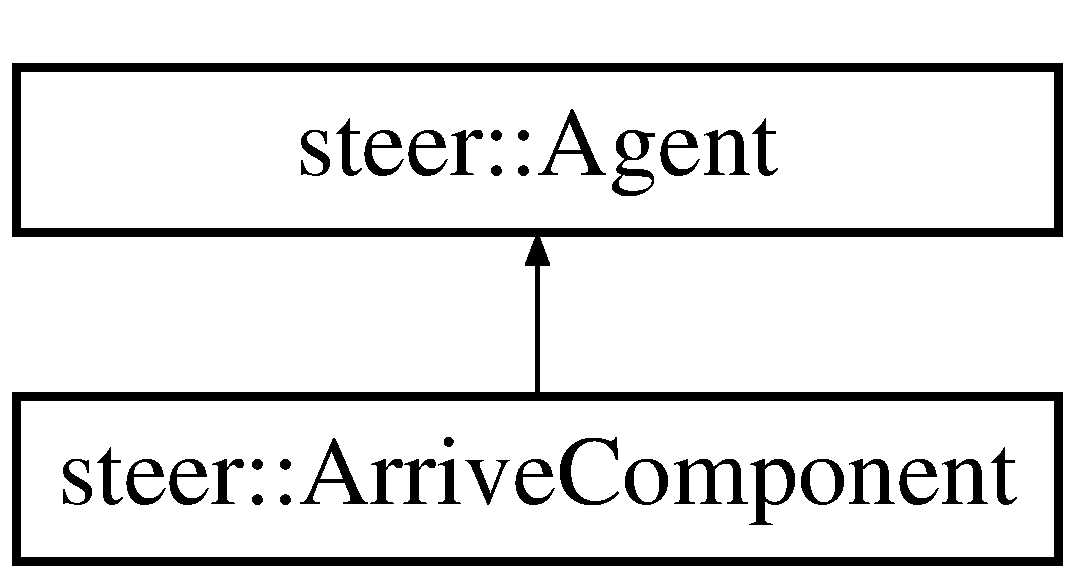
\includegraphics[height=2.000000cm]{classsteer_1_1_arrive_component}
\end{center}
\end{figure}
\subsection*{Public Member Functions}
\begin{DoxyCompactItemize}
\item 
\hypertarget{classsteer_1_1_arrive_component_a8639213b1e9236016f870853aba5e9ea}{{\bfseries Arrive\-Component} (\hyperlink{structsteer_1_1_behavior_parameters}{steer\-::\-Behavior\-Parameters} $\ast$params)}\label{classsteer_1_1_arrive_component_a8639213b1e9236016f870853aba5e9ea}

\item 
void \hyperlink{classsteer_1_1_arrive_component_a181c718e442f1b94f7318c1ea04d21a7}{set\-Weight} (const float weight)
\begin{DoxyCompactList}\small\item\em Set the value of the weight multiplier for the Arrive component. \end{DoxyCompactList}\item 
\hypertarget{classsteer_1_1_arrive_component_a9dff419ecb7381ef3348431c745d6846}{float \hyperlink{classsteer_1_1_arrive_component_a9dff419ecb7381ef3348431c745d6846}{get\-Weight} () const }\label{classsteer_1_1_arrive_component_a9dff419ecb7381ef3348431c745d6846}

\begin{DoxyCompactList}\small\item\em Get the value of the weight multiplier for the Arrive component. \end{DoxyCompactList}\item 
\hypertarget{classsteer_1_1_arrive_component_aa0b020261892f45064b4b0a912832a20}{void \hyperlink{classsteer_1_1_arrive_component_aa0b020261892f45064b4b0a912832a20}{set\-Rotation} (float r)}\label{classsteer_1_1_arrive_component_aa0b020261892f45064b4b0a912832a20}

\begin{DoxyCompactList}\small\item\em Set the value of the Arrive component rotation. \end{DoxyCompactList}\item 
\hypertarget{classsteer_1_1_arrive_component_aafe66a1cd22027b633173f3f08a7d4cc}{float \hyperlink{classsteer_1_1_arrive_component_aafe66a1cd22027b633173f3f08a7d4cc}{get\-Rotation} ()}\label{classsteer_1_1_arrive_component_aafe66a1cd22027b633173f3f08a7d4cc}

\begin{DoxyCompactList}\small\item\em Get the value of the Arrive component rotation. \end{DoxyCompactList}\item 
virtual bool \hyperlink{classsteer_1_1_arrive_component_ac904acaeee6865089e3255cf8d7390ce}{on} (\hyperlink{namespacesteer_afe6e72f8f8088962727051501181acbe}{steer\-::behavior\-Type} behavior)
\begin{DoxyCompactList}\small\item\em This pure virtual function tests if a specific bit of m\-\_\-i\-Flags is set using bitwise operations. Must be overridden in derived classes. \end{DoxyCompactList}\item 
\hypertarget{classsteer_1_1_arrive_component_aa9932b69649263979a3c3c6f6cc0e9ca}{void {\bfseries arrive\-On} ()}\label{classsteer_1_1_arrive_component_aa9932b69649263979a3c3c6f6cc0e9ca}

\item 
\hypertarget{classsteer_1_1_arrive_component_a68af4a92285c2fc0e4701592425f0ff3}{bool {\bfseries is\-Arrive\-On} ()}\label{classsteer_1_1_arrive_component_a68af4a92285c2fc0e4701592425f0ff3}

\item 
\hypertarget{classsteer_1_1_arrive_component_a0980ff65929a80b305076467fd99faa5}{void {\bfseries arrive\-Off} ()}\label{classsteer_1_1_arrive_component_a0980ff65929a80b305076467fd99faa5}

\item 
\hypertarget{classsteer_1_1_arrive_component_a8ec6d52fe9f21b59aa2388b04269620b}{bool {\bfseries target\-Acquired} ()}\label{classsteer_1_1_arrive_component_a8ec6d52fe9f21b59aa2388b04269620b}

\item 
\hypertarget{classsteer_1_1_arrive_component_ad71d15383edb2b3b40ca9bc8552e31e5}{virtual \hyperlink{structsteer_1_1_vector2}{Vector2} \hyperlink{classsteer_1_1_arrive_component_ad71d15383edb2b3b40ca9bc8552e31e5}{Calculate} ()}\label{classsteer_1_1_arrive_component_ad71d15383edb2b3b40ca9bc8552e31e5}

\begin{DoxyCompactList}\small\item\em A pure virtual method for calculating the steering vector. \end{DoxyCompactList}\item 
\hypertarget{classsteer_1_1_arrive_component_a8ef75e32bd3c2a414e21483eabd12d89}{void {\bfseries Update} (float dt)}\label{classsteer_1_1_arrive_component_a8ef75e32bd3c2a414e21483eabd12d89}

\end{DoxyCompactItemize}
\subsection*{Additional Inherited Members}


\subsection{Detailed Description}
An example implementation of the arrive steering behavior. The agent will seek the target with a dampened arrival. 

\subsection{Member Function Documentation}
\hypertarget{classsteer_1_1_arrive_component_ac904acaeee6865089e3255cf8d7390ce}{\index{steer\-::\-Arrive\-Component@{steer\-::\-Arrive\-Component}!on@{on}}
\index{on@{on}!steer::ArriveComponent@{steer\-::\-Arrive\-Component}}
\subsubsection[{on}]{\setlength{\rightskip}{0pt plus 5cm}virtual bool steer\-::\-Arrive\-Component\-::on (
\begin{DoxyParamCaption}
\item[{{\bf steer\-::behavior\-Type}}]{behavior}
\end{DoxyParamCaption}
)\hspace{0.3cm}{\ttfamily [inline]}, {\ttfamily [virtual]}}}\label{classsteer_1_1_arrive_component_ac904acaeee6865089e3255cf8d7390ce}


This pure virtual function tests if a specific bit of m\-\_\-i\-Flags is set using bitwise operations. Must be overridden in derived classes. 


\begin{DoxyParams}{Parameters}
{\em behavior} & -\/ enum behavior\-Type. \\
\hline
\end{DoxyParams}


Implements \hyperlink{classsteer_1_1_agent_a707204e49e6519c7a8ea0f3ded608d98}{steer\-::\-Agent}.

\hypertarget{classsteer_1_1_arrive_component_a181c718e442f1b94f7318c1ea04d21a7}{\index{steer\-::\-Arrive\-Component@{steer\-::\-Arrive\-Component}!set\-Weight@{set\-Weight}}
\index{set\-Weight@{set\-Weight}!steer::ArriveComponent@{steer\-::\-Arrive\-Component}}
\subsubsection[{set\-Weight}]{\setlength{\rightskip}{0pt plus 5cm}void steer\-::\-Arrive\-Component\-::set\-Weight (
\begin{DoxyParamCaption}
\item[{const float}]{weight}
\end{DoxyParamCaption}
)\hspace{0.3cm}{\ttfamily [inline]}}}\label{classsteer_1_1_arrive_component_a181c718e442f1b94f7318c1ea04d21a7}


Set the value of the weight multiplier for the Arrive component. 


\begin{DoxyParams}{Parameters}
{\em weight} & -\/ a plain old float. \\
\hline
\end{DoxyParams}


The documentation for this class was generated from the following files\-:\begin{DoxyCompactItemize}
\item 
include/steeriously/components/Arrive\-Component.\-hpp\item 
src/steeriously/components/Arrive\-Component.\-cpp\end{DoxyCompactItemize}

\hypertarget{structsteer_1_1_behavior_parameters}{\section{steer\-:\-:Behavior\-Parameters Struct Reference}
\label{structsteer_1_1_behavior_parameters}\index{steer\-::\-Behavior\-Parameters@{steer\-::\-Behavior\-Parameters}}
}


Data table with default values used to define variables for guiding steerable objects (agents).  




{\ttfamily \#include $<$Behavior\-Data.\-hpp$>$}

\subsection*{Public Attributes}
\begin{DoxyCompactItemize}
\item 
\hypertarget{structsteer_1_1_behavior_parameters_aadb118c141d8c0175bedc20777803c30}{\hyperlink{structsteer_1_1_vector2}{steer\-::\-Vector2} {\bfseries position} = \hyperlink{structsteer_1_1_vector2}{steer\-::\-Vector2}(0.\-0, 0.\-0)}\label{structsteer_1_1_behavior_parameters_aadb118c141d8c0175bedc20777803c30}

\item 
\hypertarget{structsteer_1_1_behavior_parameters_a1eb451a42b331aa2341b1dea9f328e04}{\hyperlink{structsteer_1_1_vector2}{steer\-::\-Vector2} {\bfseries velocity} = \hyperlink{structsteer_1_1_vector2}{steer\-::\-Vector2}(0.\-0, 0.\-0)}\label{structsteer_1_1_behavior_parameters_a1eb451a42b331aa2341b1dea9f328e04}

\item 
\hypertarget{structsteer_1_1_behavior_parameters_a2c7064895bba7fc1ccc51efaa44f6662}{\hyperlink{structsteer_1_1_vector2}{steer\-::\-Vector2} {\bfseries heading} = \hyperlink{structsteer_1_1_vector2}{steer\-::\-Vector2}(1.\-0, 1.\-0)}\label{structsteer_1_1_behavior_parameters_a2c7064895bba7fc1ccc51efaa44f6662}

\item 
\hypertarget{structsteer_1_1_behavior_parameters_a81873c897393052dd0b803d8fc240788}{\hyperlink{structsteer_1_1_vector2}{steer\-::\-Vector2} {\bfseries side} = \hyperlink{classsteer_1_1_vector_math_aa2820b8424b7d01bcbaf877d05108fd2}{steer\-::\-Vector\-Math\-::perpendicular}(\hyperlink{structsteer_1_1_vector2}{steer\-::\-Vector2}(1.\-0, 1.\-0))}\label{structsteer_1_1_behavior_parameters_a81873c897393052dd0b803d8fc240788}

\item 
\hypertarget{structsteer_1_1_behavior_parameters_acb0b4440984dc6a8d94881bd4e347915}{float {\bfseries radius} = 50.f}\label{structsteer_1_1_behavior_parameters_acb0b4440984dc6a8d94881bd4e347915}

\item 
\hypertarget{structsteer_1_1_behavior_parameters_a5501930734d0c68b7aea3f6d8161d29d}{float {\bfseries mass} = 1.f}\label{structsteer_1_1_behavior_parameters_a5501930734d0c68b7aea3f6d8161d29d}

\item 
\hypertarget{structsteer_1_1_behavior_parameters_aa35f968812b162cd6cf429741c85b5d3}{unsigned int {\bfseries Num\-Agents} = 1}\label{structsteer_1_1_behavior_parameters_aa35f968812b162cd6cf429741c85b5d3}

\item 
\hypertarget{structsteer_1_1_behavior_parameters_acf805248354889ba068972cb97bbd9a5}{float {\bfseries neighborhood\-Radius} = 100.f}\label{structsteer_1_1_behavior_parameters_acf805248354889ba068972cb97bbd9a5}

\item 
\hypertarget{structsteer_1_1_behavior_parameters_a7c07b3201c7c07ab03a66763b319b143}{float {\bfseries Safe\-Distance} = 100.f}\label{structsteer_1_1_behavior_parameters_a7c07b3201c7c07ab03a66763b319b143}

\item 
\hypertarget{structsteer_1_1_behavior_parameters_a56704d090cdc418a38e735e5acf974af}{float {\bfseries Threat\-Range} = 100.f}\label{structsteer_1_1_behavior_parameters_a56704d090cdc418a38e735e5acf974af}

\item 
\hypertarget{structsteer_1_1_behavior_parameters_a2b37c3d3433688b033ca9faf060e0a92}{Uint32 {\bfseries deceleration} = steer\-::\-Deceleration\-::fast}\label{structsteer_1_1_behavior_parameters_a2b37c3d3433688b033ca9faf060e0a92}

\item 
\hypertarget{structsteer_1_1_behavior_parameters_a5a959890c9378786a79c381788c5d132}{float {\bfseries Deceleration\-Tweaker} = 0.\-3f}\label{structsteer_1_1_behavior_parameters_a5a959890c9378786a79c381788c5d132}

\item 
\hypertarget{structsteer_1_1_behavior_parameters_a53ebf58e2a16e6f13ef7f0076648913d}{Uint32 {\bfseries Summing\-Method} = steer\-::summing\-Method\-::weighted\-Sum}\label{structsteer_1_1_behavior_parameters_a53ebf58e2a16e6f13ef7f0076648913d}

\item 
\hypertarget{structsteer_1_1_behavior_parameters_a10b5bfa4a42846422dc459e1d358b027}{unsigned int {\bfseries Num\-Obstacles} = 2}\label{structsteer_1_1_behavior_parameters_a10b5bfa4a42846422dc459e1d358b027}

\item 
\hypertarget{structsteer_1_1_behavior_parameters_a0ca8791227f209f182036e8fceae8469}{float {\bfseries Min\-Obstacle\-Radius} = 10}\label{structsteer_1_1_behavior_parameters_a0ca8791227f209f182036e8fceae8469}

\item 
\hypertarget{structsteer_1_1_behavior_parameters_ad39f6249e4599a8175c6119b6da63feb}{float {\bfseries Max\-Obstacle\-Radius} = 30}\label{structsteer_1_1_behavior_parameters_ad39f6249e4599a8175c6119b6da63feb}

\item 
\hypertarget{structsteer_1_1_behavior_parameters_a30090089b613b7c81cf8e869c5f719b2}{float {\bfseries Steering\-Force\-Tweaker} = 200.f}\label{structsteer_1_1_behavior_parameters_a30090089b613b7c81cf8e869c5f719b2}

\item 
\hypertarget{structsteer_1_1_behavior_parameters_a0b3505971141c966cea82849cbdbc8c5}{float {\bfseries Steering\-Force} = 2.f}\label{structsteer_1_1_behavior_parameters_a0b3505971141c966cea82849cbdbc8c5}

\item 
\hypertarget{structsteer_1_1_behavior_parameters_ad39b84fe7303200b17adf66bbf9bb097}{float {\bfseries Max\-Speed} = 100.f}\label{structsteer_1_1_behavior_parameters_ad39b84fe7303200b17adf66bbf9bb097}

\item 
\hypertarget{structsteer_1_1_behavior_parameters_a0a0fcced2fb5ecd2159670d7af538682}{float {\bfseries Max\-Force} = 400.f}\label{structsteer_1_1_behavior_parameters_a0a0fcced2fb5ecd2159670d7af538682}

\item 
\hypertarget{structsteer_1_1_behavior_parameters_a5bfbcac3e4f53bd8a3c9874a95ba0e26}{float {\bfseries Max\-Turn\-Rate} = 10.f}\label{structsteer_1_1_behavior_parameters_a5bfbcac3e4f53bd8a3c9874a95ba0e26}

\item 
\hypertarget{structsteer_1_1_behavior_parameters_a3136bcf0f151324bf74cec8810245eba}{float {\bfseries Vehicle\-Mass} = 1.f}\label{structsteer_1_1_behavior_parameters_a3136bcf0f151324bf74cec8810245eba}

\item 
\hypertarget{structsteer_1_1_behavior_parameters_a6d4e89e50ee97d7584c095c9858de08a}{float {\bfseries Vehicle\-Scale} = 1.f}\label{structsteer_1_1_behavior_parameters_a6d4e89e50ee97d7584c095c9858de08a}

\item 
\hypertarget{structsteer_1_1_behavior_parameters_a71122501ffe350cbe9e53596c56f9bb6}{float {\bfseries Separation\-Weight} = 1.f}\label{structsteer_1_1_behavior_parameters_a71122501ffe350cbe9e53596c56f9bb6}

\item 
\hypertarget{structsteer_1_1_behavior_parameters_acb9709736641e406373e3ee18d7f9457}{float {\bfseries Alignment\-Weight} = 10.f}\label{structsteer_1_1_behavior_parameters_acb9709736641e406373e3ee18d7f9457}

\item 
\hypertarget{structsteer_1_1_behavior_parameters_ad8342650239c72f5e95603d5707853e9}{float {\bfseries Cohesion\-Weight} = 10.f}\label{structsteer_1_1_behavior_parameters_ad8342650239c72f5e95603d5707853e9}

\item 
\hypertarget{structsteer_1_1_behavior_parameters_a7a7e38a51b6577a60f00bc7957e3ebba}{float {\bfseries Obstacle\-Avoidance\-Weight} = 10.f}\label{structsteer_1_1_behavior_parameters_a7a7e38a51b6577a60f00bc7957e3ebba}

\item 
\hypertarget{structsteer_1_1_behavior_parameters_a12097114a8d1aefcf1c8eca349245d2c}{float {\bfseries Wall\-Avoidance\-Weight} = 20.f}\label{structsteer_1_1_behavior_parameters_a12097114a8d1aefcf1c8eca349245d2c}

\item 
\hypertarget{structsteer_1_1_behavior_parameters_aa7d28b6fb28c663138d6d61f287e478b}{float {\bfseries Wander\-Weight} = 2.f}\label{structsteer_1_1_behavior_parameters_aa7d28b6fb28c663138d6d61f287e478b}

\item 
\hypertarget{structsteer_1_1_behavior_parameters_a18abefa9982768f77a18289c2fe50b61}{float {\bfseries Seek\-Weight} = 1.f}\label{structsteer_1_1_behavior_parameters_a18abefa9982768f77a18289c2fe50b61}

\item 
\hypertarget{structsteer_1_1_behavior_parameters_ae407a32512da2db06760d888478feb53}{float {\bfseries Flee\-Weight} = 1.f}\label{structsteer_1_1_behavior_parameters_ae407a32512da2db06760d888478feb53}

\item 
\hypertarget{structsteer_1_1_behavior_parameters_aee7f26aaf64fea7aa316eca05313445f}{float {\bfseries Arrive\-Weight} = 1.f}\label{structsteer_1_1_behavior_parameters_aee7f26aaf64fea7aa316eca05313445f}

\item 
\hypertarget{structsteer_1_1_behavior_parameters_aff4e3ff56c2219105af6fd07f700b71f}{float {\bfseries Pursuit\-Weight} = 1.f}\label{structsteer_1_1_behavior_parameters_aff4e3ff56c2219105af6fd07f700b71f}

\item 
\hypertarget{structsteer_1_1_behavior_parameters_af5224d6272c4fb8a8e8bb12a4ea82573}{float {\bfseries Offset\-Pursuit\-Weight} = 1.f}\label{structsteer_1_1_behavior_parameters_af5224d6272c4fb8a8e8bb12a4ea82573}

\item 
\hypertarget{structsteer_1_1_behavior_parameters_ac95564e74c40c7cb0828f61df50058b8}{float {\bfseries Interpose\-Weight} = 1.f}\label{structsteer_1_1_behavior_parameters_ac95564e74c40c7cb0828f61df50058b8}

\item 
\hypertarget{structsteer_1_1_behavior_parameters_ad81a43119ffa7efc0660a3d7d1ec914b}{float {\bfseries Hide\-Weight} = 1.f}\label{structsteer_1_1_behavior_parameters_ad81a43119ffa7efc0660a3d7d1ec914b}

\item 
\hypertarget{structsteer_1_1_behavior_parameters_a252349a5bb4b3b206d29dc192e358b1f}{float {\bfseries Evade\-Weight} = 0.\-01f}\label{structsteer_1_1_behavior_parameters_a252349a5bb4b3b206d29dc192e358b1f}

\item 
\hypertarget{structsteer_1_1_behavior_parameters_abbf3dc49401940ffe6aaac07c9d2379a}{float {\bfseries Follow\-Path\-Weight} = 10.f}\label{structsteer_1_1_behavior_parameters_abbf3dc49401940ffe6aaac07c9d2379a}

\item 
\hypertarget{structsteer_1_1_behavior_parameters_a9eb3e6693c273e5eebd5d8181608b588}{float {\bfseries wander\-Radius} = 100.f}\label{structsteer_1_1_behavior_parameters_a9eb3e6693c273e5eebd5d8181608b588}

\item 
\hypertarget{structsteer_1_1_behavior_parameters_ab591c887f460e163136db7e908bc8b6f}{float {\bfseries wander\-Distance} = 0.\-001f}\label{structsteer_1_1_behavior_parameters_ab591c887f460e163136db7e908bc8b6f}

\item 
\hypertarget{structsteer_1_1_behavior_parameters_a56c5f6bcf76d9e3a4f6164c480b69464}{float {\bfseries wander\-Jitter\-Per\-Second} = 360.f}\label{structsteer_1_1_behavior_parameters_a56c5f6bcf76d9e3a4f6164c480b69464}

\item 
\hypertarget{structsteer_1_1_behavior_parameters_a15b6a80c0553a533c01b72690738ab8c}{float {\bfseries waypoint\-Seek\-Distance} = 20.f}\label{structsteer_1_1_behavior_parameters_a15b6a80c0553a533c01b72690738ab8c}

\item 
\hypertarget{structsteer_1_1_behavior_parameters_a697f59d8d7c765b1da478668861c28aa}{float {\bfseries waypoint\-Seek\-Distance\-Squared} = waypoint\-Seek\-Distance$\ast$waypoint\-Seek\-Distance}\label{structsteer_1_1_behavior_parameters_a697f59d8d7c765b1da478668861c28aa}

\item 
\hypertarget{structsteer_1_1_behavior_parameters_a416529f35c516c3854c9309f5e3bda53}{float {\bfseries View\-Distance} = 100.f}\label{structsteer_1_1_behavior_parameters_a416529f35c516c3854c9309f5e3bda53}

\item 
\hypertarget{structsteer_1_1_behavior_parameters_a04178942eed91370ae2912c20f0b6f60}{float {\bfseries Min\-Detection\-Box\-Length} = 40.f}\label{structsteer_1_1_behavior_parameters_a04178942eed91370ae2912c20f0b6f60}

\item 
\hypertarget{structsteer_1_1_behavior_parameters_a6d3cf3e444e26f56f8e7bd97374ef114}{float {\bfseries Wall\-Detection\-Feeler\-Length} = 40.f}\label{structsteer_1_1_behavior_parameters_a6d3cf3e444e26f56f8e7bd97374ef114}

\end{DoxyCompactItemize}


\subsection{Detailed Description}
Data table with default values used to define variables for guiding steerable objects (agents). 

The documentation for this struct was generated from the following file\-:\begin{DoxyCompactItemize}
\item 
include/steeriously/Behavior\-Data.\-hpp\end{DoxyCompactItemize}

\hypertarget{classsteer_1_1_evade_component}{\section{steer\-:\-:Evade\-Component Class Reference}
\label{classsteer_1_1_evade_component}\index{steer\-::\-Evade\-Component@{steer\-::\-Evade\-Component}}
}


An example implementation of the evasion steering behavior. The agent will flee from the target while predicting it's trajectory.  




{\ttfamily \#include $<$Evade\-Component.\-hpp$>$}

Inheritance diagram for steer\-:\-:Evade\-Component\-:\begin{figure}[H]
\begin{center}
\leavevmode
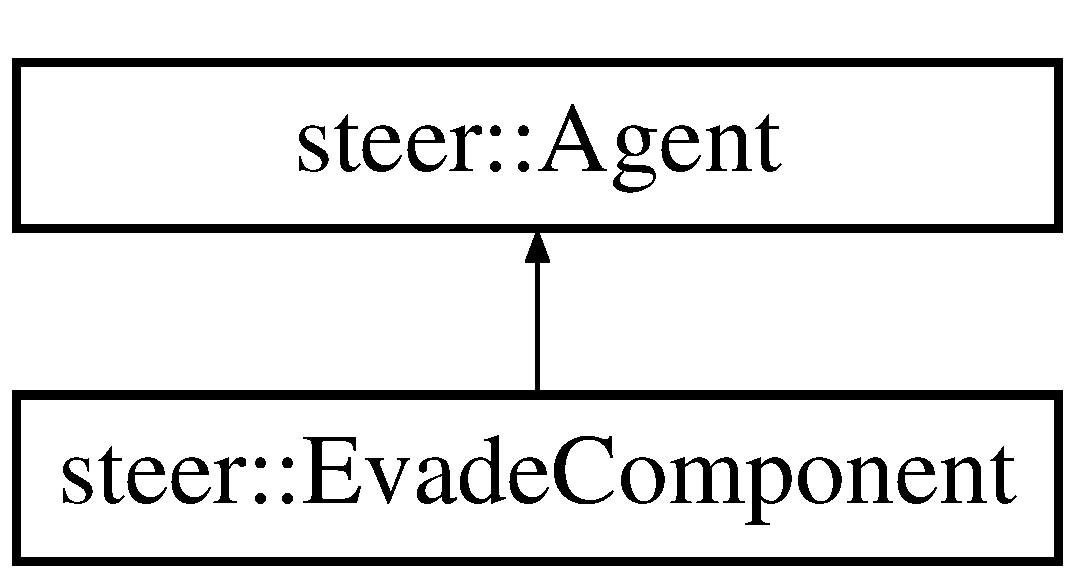
\includegraphics[height=2.000000cm]{classsteer_1_1_evade_component}
\end{center}
\end{figure}
\subsection*{Public Member Functions}
\begin{DoxyCompactItemize}
\item 
\hypertarget{classsteer_1_1_evade_component_a56c6cc0f6e8e819ab3aba63b461a897b}{{\bfseries Evade\-Component} (\hyperlink{structsteer_1_1_behavior_parameters}{steer\-::\-Behavior\-Parameters} $\ast$params)}\label{classsteer_1_1_evade_component_a56c6cc0f6e8e819ab3aba63b461a897b}

\item 
void \hyperlink{classsteer_1_1_evade_component_aa4508855f3d115907b2706d9a2349755}{set\-Weight} (const float weight)
\begin{DoxyCompactList}\small\item\em Set the value of the weight multiplier for the Evade component. \end{DoxyCompactList}\item 
\hypertarget{classsteer_1_1_evade_component_af8e0bea9a0297bb66e73a04e7aaa4a3d}{float \hyperlink{classsteer_1_1_evade_component_af8e0bea9a0297bb66e73a04e7aaa4a3d}{get\-Weight} () const }\label{classsteer_1_1_evade_component_af8e0bea9a0297bb66e73a04e7aaa4a3d}

\begin{DoxyCompactList}\small\item\em Get the value of the weight multiplier for the Evade component. \end{DoxyCompactList}\item 
\hypertarget{classsteer_1_1_evade_component_a525a0526444c1ae02938f69ced7cf1c2}{void \hyperlink{classsteer_1_1_evade_component_a525a0526444c1ae02938f69ced7cf1c2}{set\-Rotation} (float r)}\label{classsteer_1_1_evade_component_a525a0526444c1ae02938f69ced7cf1c2}

\begin{DoxyCompactList}\small\item\em Set the value of the Evade component rotation. \end{DoxyCompactList}\item 
\hypertarget{classsteer_1_1_evade_component_a7567625165b0e98b95b5a6080f134e89}{float \hyperlink{classsteer_1_1_evade_component_a7567625165b0e98b95b5a6080f134e89}{get\-Rotation} ()}\label{classsteer_1_1_evade_component_a7567625165b0e98b95b5a6080f134e89}

\begin{DoxyCompactList}\small\item\em Get the value of the Evade component rotation. \end{DoxyCompactList}\item 
virtual bool \hyperlink{classsteer_1_1_evade_component_a7e71d5e7024ed7bce4624c831477f67b}{on} (\hyperlink{namespacesteer_afe6e72f8f8088962727051501181acbe}{steer\-::behavior\-Type} behavior)
\begin{DoxyCompactList}\small\item\em This pure virtual function tests if a specific bit of m\-\_\-i\-Flags is set using bitwise operations. Must be overridden in derived classes. \end{DoxyCompactList}\item 
\hypertarget{classsteer_1_1_evade_component_a9a2c4af52abc1eca52f43ff3a852be92}{void {\bfseries evade\-On} ()}\label{classsteer_1_1_evade_component_a9a2c4af52abc1eca52f43ff3a852be92}

\item 
\hypertarget{classsteer_1_1_evade_component_aa1d283de78d3327b9d711daf5303868b}{bool {\bfseries is\-Evade\-On} ()}\label{classsteer_1_1_evade_component_aa1d283de78d3327b9d711daf5303868b}

\item 
\hypertarget{classsteer_1_1_evade_component_aaa5e5db2dbc30c458042616ac8523c54}{void {\bfseries evade\-Off} ()}\label{classsteer_1_1_evade_component_aaa5e5db2dbc30c458042616ac8523c54}

\item 
\hypertarget{classsteer_1_1_evade_component_ac69216383eb27bd5841fc86fc08e0e77}{void {\bfseries set\-Target\-Agent} (\hyperlink{classsteer_1_1_agent}{steer\-::\-Agent} $\ast$a)}\label{classsteer_1_1_evade_component_ac69216383eb27bd5841fc86fc08e0e77}

\item 
\hypertarget{classsteer_1_1_evade_component_aca2324dcca0d3a1d9e435990c1adb299}{\hyperlink{classsteer_1_1_agent}{steer\-::\-Agent} $\ast$ {\bfseries get\-Target\-Agent} () const }\label{classsteer_1_1_evade_component_aca2324dcca0d3a1d9e435990c1adb299}

\item 
\hypertarget{classsteer_1_1_evade_component_a480a701424072758ba65458f1dfa5fe1}{virtual \hyperlink{structsteer_1_1_vector2}{Vector2} \hyperlink{classsteer_1_1_evade_component_a480a701424072758ba65458f1dfa5fe1}{Calculate} ()}\label{classsteer_1_1_evade_component_a480a701424072758ba65458f1dfa5fe1}

\begin{DoxyCompactList}\small\item\em A pure virtual method for calculating the steering vector. \end{DoxyCompactList}\item 
\hypertarget{classsteer_1_1_evade_component_a1a7516399d08da295f5132c016c4b300}{void {\bfseries Update} (float dt)}\label{classsteer_1_1_evade_component_a1a7516399d08da295f5132c016c4b300}

\end{DoxyCompactItemize}
\subsection*{Additional Inherited Members}


\subsection{Detailed Description}
An example implementation of the evasion steering behavior. The agent will flee from the target while predicting it's trajectory. 

\subsection{Member Function Documentation}
\hypertarget{classsteer_1_1_evade_component_a7e71d5e7024ed7bce4624c831477f67b}{\index{steer\-::\-Evade\-Component@{steer\-::\-Evade\-Component}!on@{on}}
\index{on@{on}!steer::EvadeComponent@{steer\-::\-Evade\-Component}}
\subsubsection[{on}]{\setlength{\rightskip}{0pt plus 5cm}virtual bool steer\-::\-Evade\-Component\-::on (
\begin{DoxyParamCaption}
\item[{{\bf steer\-::behavior\-Type}}]{behavior}
\end{DoxyParamCaption}
)\hspace{0.3cm}{\ttfamily [inline]}, {\ttfamily [virtual]}}}\label{classsteer_1_1_evade_component_a7e71d5e7024ed7bce4624c831477f67b}


This pure virtual function tests if a specific bit of m\-\_\-i\-Flags is set using bitwise operations. Must be overridden in derived classes. 


\begin{DoxyParams}{Parameters}
{\em behavior} & -\/ enum behavior\-Type. \\
\hline
\end{DoxyParams}


Implements \hyperlink{classsteer_1_1_agent_a707204e49e6519c7a8ea0f3ded608d98}{steer\-::\-Agent}.

\hypertarget{classsteer_1_1_evade_component_aa4508855f3d115907b2706d9a2349755}{\index{steer\-::\-Evade\-Component@{steer\-::\-Evade\-Component}!set\-Weight@{set\-Weight}}
\index{set\-Weight@{set\-Weight}!steer::EvadeComponent@{steer\-::\-Evade\-Component}}
\subsubsection[{set\-Weight}]{\setlength{\rightskip}{0pt plus 5cm}void steer\-::\-Evade\-Component\-::set\-Weight (
\begin{DoxyParamCaption}
\item[{const float}]{weight}
\end{DoxyParamCaption}
)\hspace{0.3cm}{\ttfamily [inline]}}}\label{classsteer_1_1_evade_component_aa4508855f3d115907b2706d9a2349755}


Set the value of the weight multiplier for the Evade component. 


\begin{DoxyParams}{Parameters}
{\em weight} & -\/ a plain old float. \\
\hline
\end{DoxyParams}


The documentation for this class was generated from the following files\-:\begin{DoxyCompactItemize}
\item 
include/steeriously/components/Evade\-Component.\-hpp\item 
src/steeriously/components/Evade\-Component.\-cpp\end{DoxyCompactItemize}

\hypertarget{classsteer_1_1_flee_component}{\section{steer\-:\-:Flee\-Component Class Reference}
\label{classsteer_1_1_flee_component}\index{steer\-::\-Flee\-Component@{steer\-::\-Flee\-Component}}
}


An example implementation of the flee steering behavior. The agent will flee from the target when it enters its threat range.  




{\ttfamily \#include $<$Flee\-Component.\-hpp$>$}

Inheritance diagram for steer\-:\-:Flee\-Component\-:\begin{figure}[H]
\begin{center}
\leavevmode
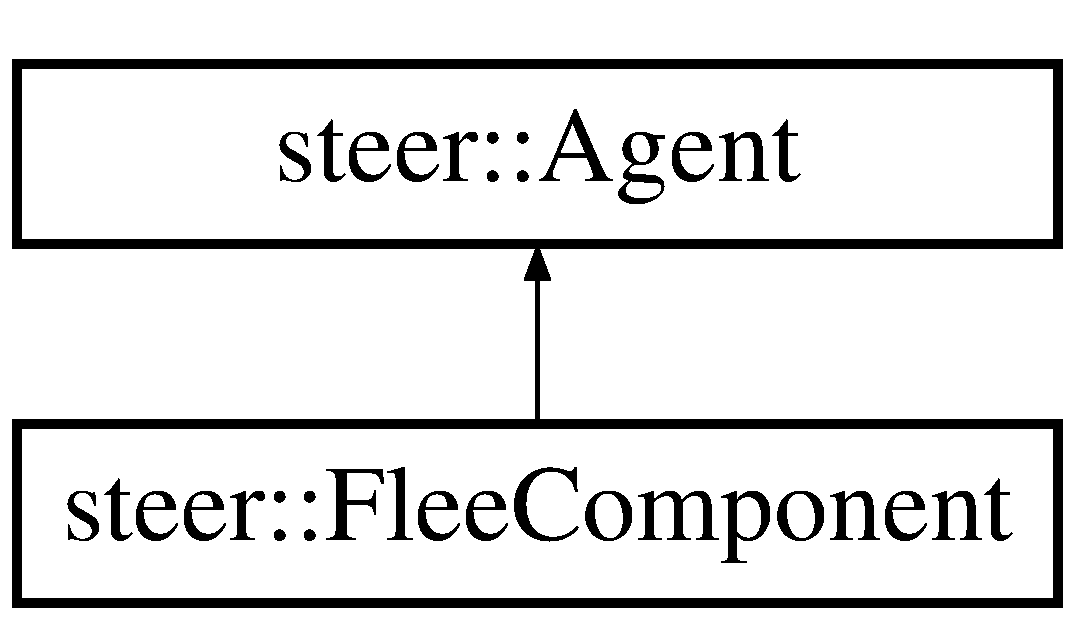
\includegraphics[height=2.000000cm]{classsteer_1_1_flee_component}
\end{center}
\end{figure}
\subsection*{Public Member Functions}
\begin{DoxyCompactItemize}
\item 
\hypertarget{classsteer_1_1_flee_component_a5d22713dafeafb40c1bbb7ef0c407ad3}{{\bfseries Flee\-Component} (\hyperlink{structsteer_1_1_behavior_parameters}{steer\-::\-Behavior\-Parameters} $\ast$params)}\label{classsteer_1_1_flee_component_a5d22713dafeafb40c1bbb7ef0c407ad3}

\item 
void \hyperlink{classsteer_1_1_flee_component_a8a0351ac86dae827867267d4e66b85ed}{set\-Weight} (const float weight)
\begin{DoxyCompactList}\small\item\em Set the value of the weight multiplier for the Flee component. \end{DoxyCompactList}\item 
\hypertarget{classsteer_1_1_flee_component_a461a45118d51c7fece0becca6b006311}{float \hyperlink{classsteer_1_1_flee_component_a461a45118d51c7fece0becca6b006311}{get\-Weight} () const }\label{classsteer_1_1_flee_component_a461a45118d51c7fece0becca6b006311}

\begin{DoxyCompactList}\small\item\em Get the value of the weight multiplier for the Flee component. \end{DoxyCompactList}\item 
\hypertarget{classsteer_1_1_flee_component_a271c3305229a8a6497ca30233ead31eb}{void \hyperlink{classsteer_1_1_flee_component_a271c3305229a8a6497ca30233ead31eb}{set\-Rotation} (float r)}\label{classsteer_1_1_flee_component_a271c3305229a8a6497ca30233ead31eb}

\begin{DoxyCompactList}\small\item\em Set the value of the Flee component rotation. \end{DoxyCompactList}\item 
\hypertarget{classsteer_1_1_flee_component_a2ec7a44b50c2afb647d7c47b0987e263}{float \hyperlink{classsteer_1_1_flee_component_a2ec7a44b50c2afb647d7c47b0987e263}{get\-Rotation} ()}\label{classsteer_1_1_flee_component_a2ec7a44b50c2afb647d7c47b0987e263}

\begin{DoxyCompactList}\small\item\em Get the value of the Flee component rotation. \end{DoxyCompactList}\item 
virtual bool \hyperlink{classsteer_1_1_flee_component_a7e344d7ea6b5b2f3e50ef7f21ec1ab10}{on} (\hyperlink{namespacesteer_afe6e72f8f8088962727051501181acbe}{steer\-::behavior\-Type} behavior)
\begin{DoxyCompactList}\small\item\em This pure virtual function tests if a specific bit of m\-\_\-i\-Flags is set using bitwise operations. Must be overridden in derived classes. \end{DoxyCompactList}\item 
\hypertarget{classsteer_1_1_flee_component_a9dcd08c721082c34c3ab64b15b52cbf7}{void {\bfseries flee\-On} ()}\label{classsteer_1_1_flee_component_a9dcd08c721082c34c3ab64b15b52cbf7}

\item 
\hypertarget{classsteer_1_1_flee_component_a6eb91968d02482207fe55da84d1c1e10}{bool {\bfseries is\-Flee\-On} ()}\label{classsteer_1_1_flee_component_a6eb91968d02482207fe55da84d1c1e10}

\item 
\hypertarget{classsteer_1_1_flee_component_a2b776b76125b6ab3212331527fd65ad9}{void {\bfseries flee\-Off} ()}\label{classsteer_1_1_flee_component_a2b776b76125b6ab3212331527fd65ad9}

\item 
\hypertarget{classsteer_1_1_flee_component_a59bc470e39187f1d8c8ee7c790139ff0}{virtual \hyperlink{structsteer_1_1_vector2}{Vector2} \hyperlink{classsteer_1_1_flee_component_a59bc470e39187f1d8c8ee7c790139ff0}{Calculate} ()}\label{classsteer_1_1_flee_component_a59bc470e39187f1d8c8ee7c790139ff0}

\begin{DoxyCompactList}\small\item\em A pure virtual method for calculating the steering vector. \end{DoxyCompactList}\item 
\hypertarget{classsteer_1_1_flee_component_ab7bde45febdd507ef92c0e1993c5d68c}{void {\bfseries Update} (float dt)}\label{classsteer_1_1_flee_component_ab7bde45febdd507ef92c0e1993c5d68c}

\end{DoxyCompactItemize}
\subsection*{Additional Inherited Members}


\subsection{Detailed Description}
An example implementation of the flee steering behavior. The agent will flee from the target when it enters its threat range. 

\subsection{Member Function Documentation}
\hypertarget{classsteer_1_1_flee_component_a7e344d7ea6b5b2f3e50ef7f21ec1ab10}{\index{steer\-::\-Flee\-Component@{steer\-::\-Flee\-Component}!on@{on}}
\index{on@{on}!steer::FleeComponent@{steer\-::\-Flee\-Component}}
\subsubsection[{on}]{\setlength{\rightskip}{0pt plus 5cm}virtual bool steer\-::\-Flee\-Component\-::on (
\begin{DoxyParamCaption}
\item[{{\bf steer\-::behavior\-Type}}]{behavior}
\end{DoxyParamCaption}
)\hspace{0.3cm}{\ttfamily [inline]}, {\ttfamily [virtual]}}}\label{classsteer_1_1_flee_component_a7e344d7ea6b5b2f3e50ef7f21ec1ab10}


This pure virtual function tests if a specific bit of m\-\_\-i\-Flags is set using bitwise operations. Must be overridden in derived classes. 


\begin{DoxyParams}{Parameters}
{\em behavior} & -\/ enum behavior\-Type. \\
\hline
\end{DoxyParams}


Implements \hyperlink{classsteer_1_1_agent_a707204e49e6519c7a8ea0f3ded608d98}{steer\-::\-Agent}.

\hypertarget{classsteer_1_1_flee_component_a8a0351ac86dae827867267d4e66b85ed}{\index{steer\-::\-Flee\-Component@{steer\-::\-Flee\-Component}!set\-Weight@{set\-Weight}}
\index{set\-Weight@{set\-Weight}!steer::FleeComponent@{steer\-::\-Flee\-Component}}
\subsubsection[{set\-Weight}]{\setlength{\rightskip}{0pt plus 5cm}void steer\-::\-Flee\-Component\-::set\-Weight (
\begin{DoxyParamCaption}
\item[{const float}]{weight}
\end{DoxyParamCaption}
)\hspace{0.3cm}{\ttfamily [inline]}}}\label{classsteer_1_1_flee_component_a8a0351ac86dae827867267d4e66b85ed}


Set the value of the weight multiplier for the Flee component. 


\begin{DoxyParams}{Parameters}
{\em weight} & -\/ a plain old float. \\
\hline
\end{DoxyParams}


The documentation for this class was generated from the following files\-:\begin{DoxyCompactItemize}
\item 
include/steeriously/components/Flee\-Component.\-hpp\item 
src/steeriously/components/Flee\-Component.\-cpp\end{DoxyCompactItemize}

\hypertarget{classsteer_1_1_flocking_component}{\section{steer\-:\-:Flocking\-Component Class Reference}
\label{classsteer_1_1_flocking_component}\index{steer\-::\-Flocking\-Component@{steer\-::\-Flocking\-Component}}
}


An example implementation of the flocking steering behavior. The agent will interact with other members of the flock utilizing alignment, separation, cohesion, and wandering behaviors.  




{\ttfamily \#include $<$Flocking\-Component.\-hpp$>$}

Inheritance diagram for steer\-:\-:Flocking\-Component\-:\begin{figure}[H]
\begin{center}
\leavevmode
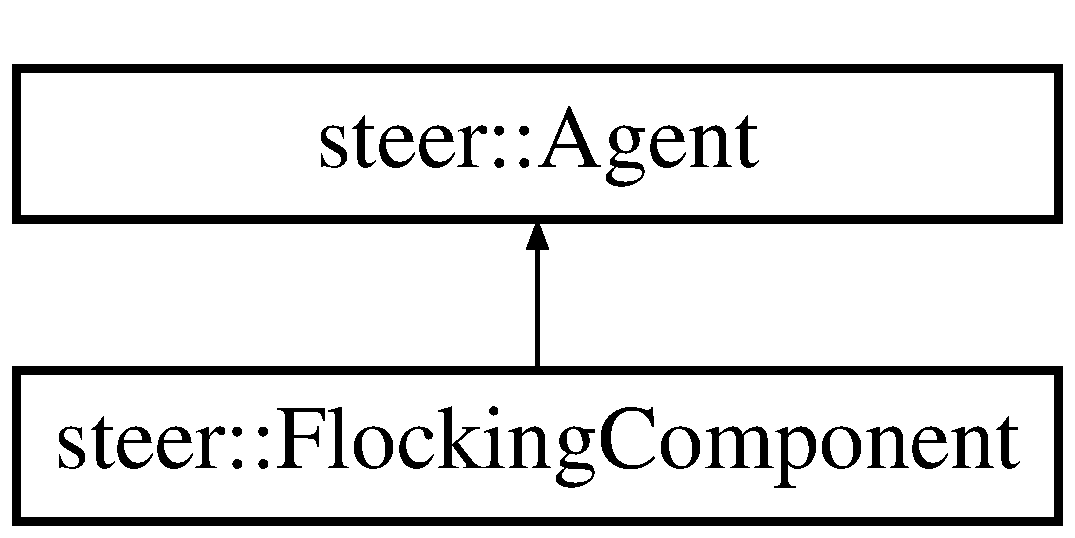
\includegraphics[height=2.000000cm]{classsteer_1_1_flocking_component}
\end{center}
\end{figure}
\subsection*{Public Member Functions}
\begin{DoxyCompactItemize}
\item 
\hypertarget{classsteer_1_1_flocking_component_a88df12e71eb24d0d8e43532f49ab38d0}{{\bfseries Flocking\-Component} (\hyperlink{structsteer_1_1_behavior_parameters}{steer\-::\-Behavior\-Parameters} $\ast$params)}\label{classsteer_1_1_flocking_component_a88df12e71eb24d0d8e43532f49ab38d0}

\item 
\hypertarget{classsteer_1_1_flocking_component_ad48b93c8e56858a90febd09b0c3f67eb}{void {\bfseries set\-Params} (\hyperlink{structsteer_1_1_behavior_parameters}{steer\-::\-Behavior\-Parameters} $\ast$params)}\label{classsteer_1_1_flocking_component_ad48b93c8e56858a90febd09b0c3f67eb}

\item 
\hypertarget{classsteer_1_1_flocking_component_a07be5adc3a5c2462d5b0ab5a9fa02638}{\hyperlink{structsteer_1_1_behavior_parameters}{steer\-::\-Behavior\-Parameters} $\ast$ {\bfseries get\-Params} ()}\label{classsteer_1_1_flocking_component_a07be5adc3a5c2462d5b0ab5a9fa02638}

\item 
\hypertarget{classsteer_1_1_flocking_component_a9f6b56e3dbe9278fe7e6dd4594e39d68}{void {\bfseries Update} (float dt)}\label{classsteer_1_1_flocking_component_a9f6b56e3dbe9278fe7e6dd4594e39d68}

\item 
\hypertarget{classsteer_1_1_flocking_component_ad0ba21cd64f3c44208f221f3d7549062}{float \hyperlink{classsteer_1_1_flocking_component_ad0ba21cd64f3c44208f221f3d7549062}{get\-Rotation} ()}\label{classsteer_1_1_flocking_component_ad0ba21cd64f3c44208f221f3d7549062}

\begin{DoxyCompactList}\small\item\em Get the value of the seek component rotation. \end{DoxyCompactList}\item 
\hypertarget{classsteer_1_1_flocking_component_aa5f923728cfe57c6fd73967e40f548e2}{void {\bfseries set\-Neighbors} (std\-::vector$<$ \hyperlink{classsteer_1_1_flocking_component}{Flocking\-Component} $\ast$ $>$ $\ast$n)}\label{classsteer_1_1_flocking_component_aa5f923728cfe57c6fd73967e40f548e2}

\item 
\hypertarget{classsteer_1_1_flocking_component_ad019771bbd11d1149d374842e33425e5}{std\-::vector$<$ \hyperlink{classsteer_1_1_flocking_component}{Flocking\-Component} $\ast$ $>$ $\ast$ {\bfseries get\-Neighbors} ()}\label{classsteer_1_1_flocking_component_ad019771bbd11d1149d374842e33425e5}

\item 
\hypertarget{classsteer_1_1_flocking_component_ab7ad010eb626dec2d0784ddef972cc2a}{void {\bfseries set\-Obstacles} (std\-::vector$<$ \hyperlink{classsteer_1_1_sphere_obstacle}{Sphere\-Obstacle} $\ast$ $>$ $\ast$o)}\label{classsteer_1_1_flocking_component_ab7ad010eb626dec2d0784ddef972cc2a}

\item 
\hypertarget{classsteer_1_1_flocking_component_a7fbfd70dcb4055fa91df97c5dcfc3821}{std\-::vector$<$ \hyperlink{classsteer_1_1_sphere_obstacle}{Sphere\-Obstacle} $\ast$ $>$ $\ast$ {\bfseries get\-Obstacles} ()}\label{classsteer_1_1_flocking_component_a7fbfd70dcb4055fa91df97c5dcfc3821}

\item 
\hypertarget{classsteer_1_1_flocking_component_ae778656b1df44de398f81c8ec66f8766}{void {\bfseries set\-Walls} (std\-::vector$<$ \hyperlink{classsteer_1_1_wall}{Wall} $\ast$ $>$ $\ast$w)}\label{classsteer_1_1_flocking_component_ae778656b1df44de398f81c8ec66f8766}

\item 
\hypertarget{classsteer_1_1_flocking_component_ae6a60ac996d1ada0145e168f541a96ef}{std\-::vector$<$ \hyperlink{classsteer_1_1_wall}{Wall} $\ast$ $>$ $\ast$ {\bfseries get\-Walls} ()}\label{classsteer_1_1_flocking_component_ae6a60ac996d1ada0145e168f541a96ef}

\item 
virtual bool \hyperlink{classsteer_1_1_flocking_component_a0d788eaec845b83503a7918e984cfd5b}{on} (\hyperlink{namespacesteer_afe6e72f8f8088962727051501181acbe}{steer\-::behavior\-Type} behavior) override
\begin{DoxyCompactList}\small\item\em This pure virtual function tests if a specific bit of m\-\_\-i\-Flags is set using bitwise operations. Must be overridden in derived classes. \end{DoxyCompactList}\item 
\hypertarget{classsteer_1_1_flocking_component_a89ac69483994c9e64f3727029f70ec58}{void {\bfseries alignment\-On} ()}\label{classsteer_1_1_flocking_component_a89ac69483994c9e64f3727029f70ec58}

\item 
\hypertarget{classsteer_1_1_flocking_component_a8adcea80a9614ae5f431cc4188c2b0d7}{void {\bfseries separation\-On} ()}\label{classsteer_1_1_flocking_component_a8adcea80a9614ae5f431cc4188c2b0d7}

\item 
\hypertarget{classsteer_1_1_flocking_component_a8d57ea0ff29d1bfae5e149e0442af54c}{void {\bfseries cohesion\-On} ()}\label{classsteer_1_1_flocking_component_a8d57ea0ff29d1bfae5e149e0442af54c}

\item 
\hypertarget{classsteer_1_1_flocking_component_aad6b6a52e2aeaaae441c4d5e0a47d455}{void {\bfseries seek\-On} ()}\label{classsteer_1_1_flocking_component_aad6b6a52e2aeaaae441c4d5e0a47d455}

\item 
\hypertarget{classsteer_1_1_flocking_component_a86f5885a8fbc8a7436420bc0f336218f}{void {\bfseries wander\-On} ()}\label{classsteer_1_1_flocking_component_a86f5885a8fbc8a7436420bc0f336218f}

\item 
\hypertarget{classsteer_1_1_flocking_component_ab9147569164325a5e1d969080dae86b2}{void {\bfseries wall\-Avoidance\-On} ()}\label{classsteer_1_1_flocking_component_ab9147569164325a5e1d969080dae86b2}

\item 
\hypertarget{classsteer_1_1_flocking_component_a6ff71635135f739469e3f43c1211b0c0}{void {\bfseries obstacle\-Avoidance\-On} ()}\label{classsteer_1_1_flocking_component_a6ff71635135f739469e3f43c1211b0c0}

\item 
\hypertarget{classsteer_1_1_flocking_component_adcce1eb15ddddbe03504b6fb04bfa7bd}{void {\bfseries cohesion\-Off} ()}\label{classsteer_1_1_flocking_component_adcce1eb15ddddbe03504b6fb04bfa7bd}

\item 
\hypertarget{classsteer_1_1_flocking_component_acc8272a36ff736c256912bf057dcb5cc}{void {\bfseries separation\-Off} ()}\label{classsteer_1_1_flocking_component_acc8272a36ff736c256912bf057dcb5cc}

\item 
\hypertarget{classsteer_1_1_flocking_component_a5a6972e642a81850ed4e12c32d604be8}{void {\bfseries alignment\-Off} ()}\label{classsteer_1_1_flocking_component_a5a6972e642a81850ed4e12c32d604be8}

\item 
\hypertarget{classsteer_1_1_flocking_component_a5082b73416b8e8541c1e774a5da4c2cc}{void {\bfseries seek\-Off} ()}\label{classsteer_1_1_flocking_component_a5082b73416b8e8541c1e774a5da4c2cc}

\item 
\hypertarget{classsteer_1_1_flocking_component_a42b04fd9d54d25a8b40cb222e042d621}{void {\bfseries wander\-Off} ()}\label{classsteer_1_1_flocking_component_a42b04fd9d54d25a8b40cb222e042d621}

\item 
\hypertarget{classsteer_1_1_flocking_component_a8c91bf47132fb9190e7c525fa23de44a}{void {\bfseries wall\-Avoidance\-Off} ()}\label{classsteer_1_1_flocking_component_a8c91bf47132fb9190e7c525fa23de44a}

\item 
\hypertarget{classsteer_1_1_flocking_component_a7f29936d46248db446153c87848e95c3}{void {\bfseries obstacle\-Avoidance\-Off} ()}\label{classsteer_1_1_flocking_component_a7f29936d46248db446153c87848e95c3}

\item 
\hypertarget{classsteer_1_1_flocking_component_a0c7f66f2f62391bd1396974dc322a12b}{bool {\bfseries is\-Cohesion\-On} ()}\label{classsteer_1_1_flocking_component_a0c7f66f2f62391bd1396974dc322a12b}

\item 
\hypertarget{classsteer_1_1_flocking_component_a0212122a315f595abda98ba2f7e0b589}{bool {\bfseries is\-Separation\-On} ()}\label{classsteer_1_1_flocking_component_a0212122a315f595abda98ba2f7e0b589}

\item 
\hypertarget{classsteer_1_1_flocking_component_a638dc9399d20ab681b45902915f2d66c}{bool {\bfseries is\-Alignment\-On} ()}\label{classsteer_1_1_flocking_component_a638dc9399d20ab681b45902915f2d66c}

\item 
\hypertarget{classsteer_1_1_flocking_component_a80d59920d01141fa32a549f77b82df12}{bool {\bfseries is\-Seek\-On} ()}\label{classsteer_1_1_flocking_component_a80d59920d01141fa32a549f77b82df12}

\item 
\hypertarget{classsteer_1_1_flocking_component_ae8f077a3c37906045d87268e7a54d80b}{bool {\bfseries is\-Wander\-On} ()}\label{classsteer_1_1_flocking_component_ae8f077a3c37906045d87268e7a54d80b}

\item 
\hypertarget{classsteer_1_1_flocking_component_a8498c8d98461720bc7dcb1260a379e59}{bool {\bfseries is\-Wall\-Avoidance\-On} ()}\label{classsteer_1_1_flocking_component_a8498c8d98461720bc7dcb1260a379e59}

\item 
\hypertarget{classsteer_1_1_flocking_component_a2b5218dcec5344286d67760872e875f5}{bool {\bfseries is\-Obstacle\-Avoidance\-On} ()}\label{classsteer_1_1_flocking_component_a2b5218dcec5344286d67760872e875f5}

\item 
\hypertarget{classsteer_1_1_flocking_component_a052f6b2e7181d69c61595c323d7eaa82}{bool {\bfseries is\-Flocking\-On} ()}\label{classsteer_1_1_flocking_component_a052f6b2e7181d69c61595c323d7eaa82}

\item 
\hypertarget{classsteer_1_1_flocking_component_a8f4122bf63050bb2beba5928b52ffceb}{void {\bfseries flocking\-On} ()}\label{classsteer_1_1_flocking_component_a8f4122bf63050bb2beba5928b52ffceb}

\item 
\hypertarget{classsteer_1_1_flocking_component_a88c5ad1cc6be0a0e196a6c9389c1171a}{void {\bfseries flocking\-Off} ()}\label{classsteer_1_1_flocking_component_a88c5ad1cc6be0a0e196a6c9389c1171a}

\item 
\hypertarget{classsteer_1_1_flocking_component_a898c7612d4be3123b547be3aa7759839}{bool {\bfseries target\-Acquired} ()}\label{classsteer_1_1_flocking_component_a898c7612d4be3123b547be3aa7759839}

\item 
\hypertarget{classsteer_1_1_flocking_component_aeb8123ba28d8d4a9df97c4f8b3f9b6c3}{virtual \hyperlink{structsteer_1_1_vector2}{Vector2} \hyperlink{classsteer_1_1_flocking_component_aeb8123ba28d8d4a9df97c4f8b3f9b6c3}{Calculate} () override}\label{classsteer_1_1_flocking_component_aeb8123ba28d8d4a9df97c4f8b3f9b6c3}

\begin{DoxyCompactList}\small\item\em A pure virtual method for calculating the steering vector. \end{DoxyCompactList}\item 
\hypertarget{classsteer_1_1_flocking_component_ae99047e5022fd6a9f03f77af94a956a9}{virtual \hyperlink{structsteer_1_1_vector2}{Vector2} {\bfseries calculate\-Weighted\-Sum} () override}\label{classsteer_1_1_flocking_component_ae99047e5022fd6a9f03f77af94a956a9}

\end{DoxyCompactItemize}
\subsection*{Additional Inherited Members}


\subsection{Detailed Description}
An example implementation of the flocking steering behavior. The agent will interact with other members of the flock utilizing alignment, separation, cohesion, and wandering behaviors. 

\subsection{Member Function Documentation}
\hypertarget{classsteer_1_1_flocking_component_a0d788eaec845b83503a7918e984cfd5b}{\index{steer\-::\-Flocking\-Component@{steer\-::\-Flocking\-Component}!on@{on}}
\index{on@{on}!steer::FlockingComponent@{steer\-::\-Flocking\-Component}}
\subsubsection[{on}]{\setlength{\rightskip}{0pt plus 5cm}virtual bool steer\-::\-Flocking\-Component\-::on (
\begin{DoxyParamCaption}
\item[{{\bf steer\-::behavior\-Type}}]{behavior}
\end{DoxyParamCaption}
)\hspace{0.3cm}{\ttfamily [inline]}, {\ttfamily [override]}, {\ttfamily [virtual]}}}\label{classsteer_1_1_flocking_component_a0d788eaec845b83503a7918e984cfd5b}


This pure virtual function tests if a specific bit of m\-\_\-i\-Flags is set using bitwise operations. Must be overridden in derived classes. 


\begin{DoxyParams}{Parameters}
{\em behavior} & -\/ enum behavior\-Type. \\
\hline
\end{DoxyParams}


Implements \hyperlink{classsteer_1_1_agent_a707204e49e6519c7a8ea0f3ded608d98}{steer\-::\-Agent}.



The documentation for this class was generated from the following files\-:\begin{DoxyCompactItemize}
\item 
include/steeriously/components/Flocking\-Component.\-hpp\item 
src/steeriously/components/Flocking\-Component.\-cpp\end{DoxyCompactItemize}

\hypertarget{classsteer_1_1_hide_component}{\section{steer\-:\-:Hide\-Component Class Reference}
\label{classsteer_1_1_hide_component}\index{steer\-::\-Hide\-Component@{steer\-::\-Hide\-Component}}
}


An example implementation of the hiding steering behavior.  




{\ttfamily \#include $<$Hide\-Component.\-hpp$>$}

Inheritance diagram for steer\-:\-:Hide\-Component\-:\begin{figure}[H]
\begin{center}
\leavevmode
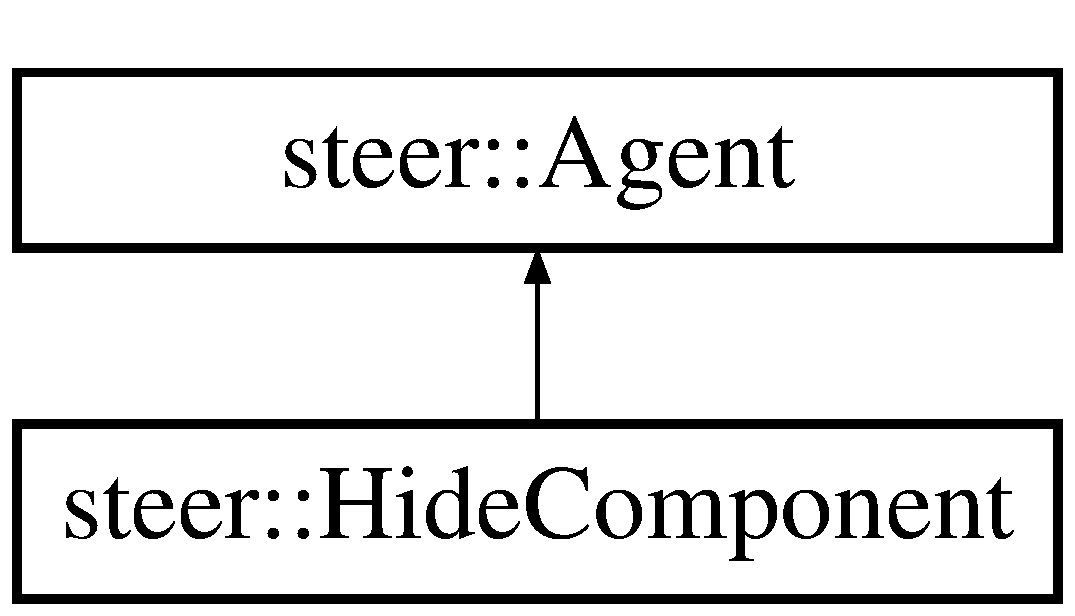
\includegraphics[height=2.000000cm]{classsteer_1_1_hide_component}
\end{center}
\end{figure}
\subsection*{Public Member Functions}
\begin{DoxyCompactItemize}
\item 
\hypertarget{classsteer_1_1_hide_component_a7d52f96991f013560c7d45889d41e2af}{{\bfseries Hide\-Component} (\hyperlink{structsteer_1_1_behavior_parameters}{steer\-::\-Behavior\-Parameters} $\ast$params)}\label{classsteer_1_1_hide_component_a7d52f96991f013560c7d45889d41e2af}

\item 
\hypertarget{classsteer_1_1_hide_component_aab92376692510d75a29e98e6c50e620c}{void {\bfseries set\-Params} (\hyperlink{structsteer_1_1_behavior_parameters}{steer\-::\-Behavior\-Parameters} $\ast$params)}\label{classsteer_1_1_hide_component_aab92376692510d75a29e98e6c50e620c}

\item 
\hypertarget{classsteer_1_1_hide_component_aa120ca55695fcb7ee3b1cc5e0d6f2424}{\hyperlink{structsteer_1_1_behavior_parameters}{steer\-::\-Behavior\-Parameters} $\ast$ {\bfseries get\-Params} ()}\label{classsteer_1_1_hide_component_aa120ca55695fcb7ee3b1cc5e0d6f2424}

\item 
void \hyperlink{classsteer_1_1_hide_component_af268ef8124fd56b3a10bd669f444739b}{set\-Weight} (const float weight)
\begin{DoxyCompactList}\small\item\em Set the value of the weight multiplier for the Hide component. \end{DoxyCompactList}\item 
\hypertarget{classsteer_1_1_hide_component_af319f306a1f3ab0196723e968257015b}{float \hyperlink{classsteer_1_1_hide_component_af319f306a1f3ab0196723e968257015b}{get\-Weight} () const }\label{classsteer_1_1_hide_component_af319f306a1f3ab0196723e968257015b}

\begin{DoxyCompactList}\small\item\em Get the value of the weight multiplier for the Hide component. \end{DoxyCompactList}\item 
\hypertarget{classsteer_1_1_hide_component_a909e034c1a9a89fc65dd184e9bcd3cb1}{void \hyperlink{classsteer_1_1_hide_component_a909e034c1a9a89fc65dd184e9bcd3cb1}{set\-Rotation} (float r)}\label{classsteer_1_1_hide_component_a909e034c1a9a89fc65dd184e9bcd3cb1}

\begin{DoxyCompactList}\small\item\em Set the value of the Hide component rotation. \end{DoxyCompactList}\item 
\hypertarget{classsteer_1_1_hide_component_a84d3f4f40129e9e5c1a323c17c2c60fe}{float \hyperlink{classsteer_1_1_hide_component_a84d3f4f40129e9e5c1a323c17c2c60fe}{get\-Rotation} ()}\label{classsteer_1_1_hide_component_a84d3f4f40129e9e5c1a323c17c2c60fe}

\begin{DoxyCompactList}\small\item\em Get the value of the Hide component rotation. \end{DoxyCompactList}\item 
\hypertarget{classsteer_1_1_hide_component_a8342f0fcf4a3f1338c5d7db797fc70f0}{void {\bfseries set\-Obstacles} (std\-::vector$<$ \hyperlink{classsteer_1_1_sphere_obstacle}{Sphere\-Obstacle} $\ast$ $>$ $\ast$o)}\label{classsteer_1_1_hide_component_a8342f0fcf4a3f1338c5d7db797fc70f0}

\item 
\hypertarget{classsteer_1_1_hide_component_ab1e6b2bfaec26bee0c81f3d316ab553d}{std\-::vector$<$ \hyperlink{classsteer_1_1_sphere_obstacle}{Sphere\-Obstacle} $\ast$ $>$ $\ast$ {\bfseries get\-Obstacles} ()}\label{classsteer_1_1_hide_component_ab1e6b2bfaec26bee0c81f3d316ab553d}

\item 
virtual bool \hyperlink{classsteer_1_1_hide_component_a64ff14630f96232381dd0fd88c1d9d04}{on} (\hyperlink{namespacesteer_afe6e72f8f8088962727051501181acbe}{steer\-::behavior\-Type} behavior)
\begin{DoxyCompactList}\small\item\em This pure virtual function tests if a specific bit of m\-\_\-i\-Flags is set using bitwise operations. Must be overridden in derived classes. \end{DoxyCompactList}\item 
\hypertarget{classsteer_1_1_hide_component_ae6cec58fe6b94fe43c9b8e434af1b7f7}{void {\bfseries Hide\-On} ()}\label{classsteer_1_1_hide_component_ae6cec58fe6b94fe43c9b8e434af1b7f7}

\item 
\hypertarget{classsteer_1_1_hide_component_afb4a0954264f650cc48d0acb500c8ff8}{bool {\bfseries is\-Hide\-On} ()}\label{classsteer_1_1_hide_component_afb4a0954264f650cc48d0acb500c8ff8}

\item 
\hypertarget{classsteer_1_1_hide_component_a94669d77ed55e882557720d1f7522a5c}{void {\bfseries Hide\-Off} ()}\label{classsteer_1_1_hide_component_a94669d77ed55e882557720d1f7522a5c}

\item 
\hypertarget{classsteer_1_1_hide_component_a0fc6f3c6b4eb749e4e88ced774f37c15}{void {\bfseries set\-Target\-Agent} (\hyperlink{classsteer_1_1_agent}{steer\-::\-Agent} $\ast$a)}\label{classsteer_1_1_hide_component_a0fc6f3c6b4eb749e4e88ced774f37c15}

\item 
\hypertarget{classsteer_1_1_hide_component_a529cb113ffc6a34f3d94e0f0d66ec42e}{\hyperlink{classsteer_1_1_agent}{steer\-::\-Agent} $\ast$ {\bfseries get\-Target\-Agent} () const }\label{classsteer_1_1_hide_component_a529cb113ffc6a34f3d94e0f0d66ec42e}

\item 
\hypertarget{classsteer_1_1_hide_component_aa52479885bacf5d24da8d480f2d7b2ff}{virtual \hyperlink{structsteer_1_1_vector2}{Vector2} \hyperlink{classsteer_1_1_hide_component_aa52479885bacf5d24da8d480f2d7b2ff}{Calculate} ()}\label{classsteer_1_1_hide_component_aa52479885bacf5d24da8d480f2d7b2ff}

\begin{DoxyCompactList}\small\item\em A pure virtual method for calculating the steering vector. \end{DoxyCompactList}\item 
\hypertarget{classsteer_1_1_hide_component_a7c07df9bbf52430c759683bc07e1e269}{void {\bfseries Update} (float dt)}\label{classsteer_1_1_hide_component_a7c07df9bbf52430c759683bc07e1e269}

\end{DoxyCompactItemize}
\subsection*{Additional Inherited Members}


\subsection{Detailed Description}
An example implementation of the hiding steering behavior. 

\subsection{Member Function Documentation}
\hypertarget{classsteer_1_1_hide_component_a64ff14630f96232381dd0fd88c1d9d04}{\index{steer\-::\-Hide\-Component@{steer\-::\-Hide\-Component}!on@{on}}
\index{on@{on}!steer::HideComponent@{steer\-::\-Hide\-Component}}
\subsubsection[{on}]{\setlength{\rightskip}{0pt plus 5cm}virtual bool steer\-::\-Hide\-Component\-::on (
\begin{DoxyParamCaption}
\item[{{\bf steer\-::behavior\-Type}}]{behavior}
\end{DoxyParamCaption}
)\hspace{0.3cm}{\ttfamily [inline]}, {\ttfamily [virtual]}}}\label{classsteer_1_1_hide_component_a64ff14630f96232381dd0fd88c1d9d04}


This pure virtual function tests if a specific bit of m\-\_\-i\-Flags is set using bitwise operations. Must be overridden in derived classes. 


\begin{DoxyParams}{Parameters}
{\em behavior} & -\/ enum behavior\-Type. \\
\hline
\end{DoxyParams}


Implements \hyperlink{classsteer_1_1_agent_a707204e49e6519c7a8ea0f3ded608d98}{steer\-::\-Agent}.

\hypertarget{classsteer_1_1_hide_component_af268ef8124fd56b3a10bd669f444739b}{\index{steer\-::\-Hide\-Component@{steer\-::\-Hide\-Component}!set\-Weight@{set\-Weight}}
\index{set\-Weight@{set\-Weight}!steer::HideComponent@{steer\-::\-Hide\-Component}}
\subsubsection[{set\-Weight}]{\setlength{\rightskip}{0pt plus 5cm}void steer\-::\-Hide\-Component\-::set\-Weight (
\begin{DoxyParamCaption}
\item[{const float}]{weight}
\end{DoxyParamCaption}
)\hspace{0.3cm}{\ttfamily [inline]}}}\label{classsteer_1_1_hide_component_af268ef8124fd56b3a10bd669f444739b}


Set the value of the weight multiplier for the Hide component. 


\begin{DoxyParams}{Parameters}
{\em weight} & -\/ a plain old float. \\
\hline
\end{DoxyParams}


The documentation for this class was generated from the following files\-:\begin{DoxyCompactItemize}
\item 
include/steeriously/components/Hide\-Component.\-hpp\item 
src/steeriously/components/Hide\-Component.\-cpp\end{DoxyCompactItemize}

\hypertarget{classsteer_1_1_interpose_component}{\section{steer\-:\-:Interpose\-Component Class Reference}
\label{classsteer_1_1_interpose_component}\index{steer\-::\-Interpose\-Component@{steer\-::\-Interpose\-Component}}
}


An example implementation of the interpose steering behavior.  




{\ttfamily \#include $<$Interpose\-Component.\-hpp$>$}

Inheritance diagram for steer\-:\-:Interpose\-Component\-:\begin{figure}[H]
\begin{center}
\leavevmode
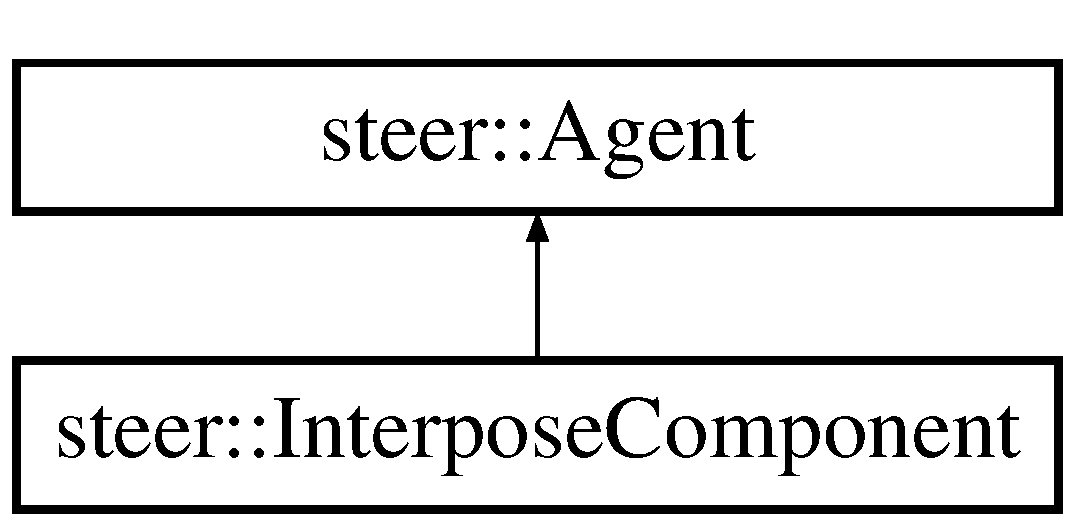
\includegraphics[height=2.000000cm]{classsteer_1_1_interpose_component}
\end{center}
\end{figure}
\subsection*{Public Member Functions}
\begin{DoxyCompactItemize}
\item 
\hypertarget{classsteer_1_1_interpose_component_a98c2fe70659f855de3de0dd2da1c849b}{{\bfseries Interpose\-Component} (\hyperlink{structsteer_1_1_behavior_parameters}{steer\-::\-Behavior\-Parameters} $\ast$params)}\label{classsteer_1_1_interpose_component_a98c2fe70659f855de3de0dd2da1c849b}

\item 
void \hyperlink{classsteer_1_1_interpose_component_acb57d889e89e0b1f9bc5acb92b620a23}{set\-Weight} (const float weight)
\begin{DoxyCompactList}\small\item\em Set the value of the weight multiplier for the Interpose component. \end{DoxyCompactList}\item 
\hypertarget{classsteer_1_1_interpose_component_ad1920f951a1b37b6070ac39ffc6bf225}{float \hyperlink{classsteer_1_1_interpose_component_ad1920f951a1b37b6070ac39ffc6bf225}{get\-Weight} () const }\label{classsteer_1_1_interpose_component_ad1920f951a1b37b6070ac39ffc6bf225}

\begin{DoxyCompactList}\small\item\em Get the value of the weight multiplier for the Interpose component. \end{DoxyCompactList}\item 
\hypertarget{classsteer_1_1_interpose_component_a83249b4d48e4434e7bb341c0b1d768b2}{void \hyperlink{classsteer_1_1_interpose_component_a83249b4d48e4434e7bb341c0b1d768b2}{set\-Rotation} (float r)}\label{classsteer_1_1_interpose_component_a83249b4d48e4434e7bb341c0b1d768b2}

\begin{DoxyCompactList}\small\item\em Set the value of the Interpose component rotation. \end{DoxyCompactList}\item 
\hypertarget{classsteer_1_1_interpose_component_a87b3dbdba7c248e1926cf110daf3dd4e}{float \hyperlink{classsteer_1_1_interpose_component_a87b3dbdba7c248e1926cf110daf3dd4e}{get\-Rotation} ()}\label{classsteer_1_1_interpose_component_a87b3dbdba7c248e1926cf110daf3dd4e}

\begin{DoxyCompactList}\small\item\em Get the value of the Interpose component rotation. \end{DoxyCompactList}\item 
virtual bool \hyperlink{classsteer_1_1_interpose_component_a0ad5f9af346843c67983d103d1e3d167}{on} (\hyperlink{namespacesteer_afe6e72f8f8088962727051501181acbe}{steer\-::behavior\-Type} behavior)
\begin{DoxyCompactList}\small\item\em This pure virtual function tests if a specific bit of m\-\_\-i\-Flags is set using bitwise operations. Must be overridden in derived classes. \end{DoxyCompactList}\item 
\hypertarget{classsteer_1_1_interpose_component_a8309a2d1d2dcae45a68d13bafb01b740}{void {\bfseries Interpose\-On} ()}\label{classsteer_1_1_interpose_component_a8309a2d1d2dcae45a68d13bafb01b740}

\item 
\hypertarget{classsteer_1_1_interpose_component_a996410c4ea8186310f5602c85f8787e8}{bool {\bfseries is\-Interpose\-On} ()}\label{classsteer_1_1_interpose_component_a996410c4ea8186310f5602c85f8787e8}

\item 
\hypertarget{classsteer_1_1_interpose_component_ad4e03f37825873f7127475dba89e0439}{void {\bfseries Interpose\-Off} ()}\label{classsteer_1_1_interpose_component_ad4e03f37825873f7127475dba89e0439}

\item 
\hypertarget{classsteer_1_1_interpose_component_a689155e2355f2e3159b8bd6f5346c491}{void {\bfseries set\-Agents} (\hyperlink{classsteer_1_1_agent}{steer\-::\-Agent} $\ast$a, \hyperlink{classsteer_1_1_agent}{steer\-::\-Agent} $\ast$b)}\label{classsteer_1_1_interpose_component_a689155e2355f2e3159b8bd6f5346c491}

\item 
\hypertarget{classsteer_1_1_interpose_component_ab30a6827567147106a3c5d148f88e24e}{void {\bfseries set\-Agent\-A} (\hyperlink{classsteer_1_1_agent}{steer\-::\-Agent} $\ast$a)}\label{classsteer_1_1_interpose_component_ab30a6827567147106a3c5d148f88e24e}

\item 
\hypertarget{classsteer_1_1_interpose_component_ad4481935cbdfbbac48855833b2aa25db}{void {\bfseries set\-Agent\-B} (\hyperlink{classsteer_1_1_agent}{steer\-::\-Agent} $\ast$b)}\label{classsteer_1_1_interpose_component_ad4481935cbdfbbac48855833b2aa25db}

\item 
\hypertarget{classsteer_1_1_interpose_component_a7e9ec67d9c5c986e819058c1b4a01586}{\hyperlink{classsteer_1_1_agent}{steer\-::\-Agent} $\ast$ {\bfseries get\-Agent\-A} () const }\label{classsteer_1_1_interpose_component_a7e9ec67d9c5c986e819058c1b4a01586}

\item 
\hypertarget{classsteer_1_1_interpose_component_ab0859ceef7d33e29ea54696ca681109c}{\hyperlink{classsteer_1_1_agent}{steer\-::\-Agent} $\ast$ {\bfseries get\-Agent\-B} () const }\label{classsteer_1_1_interpose_component_ab0859ceef7d33e29ea54696ca681109c}

\item 
\hypertarget{classsteer_1_1_interpose_component_a39236f55299e42b334eaf6fd7cc35da2}{virtual \hyperlink{structsteer_1_1_vector2}{Vector2} \hyperlink{classsteer_1_1_interpose_component_a39236f55299e42b334eaf6fd7cc35da2}{Calculate} ()}\label{classsteer_1_1_interpose_component_a39236f55299e42b334eaf6fd7cc35da2}

\begin{DoxyCompactList}\small\item\em A pure virtual method for calculating the steering vector. \end{DoxyCompactList}\item 
\hypertarget{classsteer_1_1_interpose_component_acd5671cafee4f1b08eef0865d6874e46}{void {\bfseries Update} (float dt)}\label{classsteer_1_1_interpose_component_acd5671cafee4f1b08eef0865d6874e46}

\end{DoxyCompactItemize}
\subsection*{Additional Inherited Members}


\subsection{Detailed Description}
An example implementation of the interpose steering behavior. 

\subsection{Member Function Documentation}
\hypertarget{classsteer_1_1_interpose_component_a0ad5f9af346843c67983d103d1e3d167}{\index{steer\-::\-Interpose\-Component@{steer\-::\-Interpose\-Component}!on@{on}}
\index{on@{on}!steer::InterposeComponent@{steer\-::\-Interpose\-Component}}
\subsubsection[{on}]{\setlength{\rightskip}{0pt plus 5cm}virtual bool steer\-::\-Interpose\-Component\-::on (
\begin{DoxyParamCaption}
\item[{{\bf steer\-::behavior\-Type}}]{behavior}
\end{DoxyParamCaption}
)\hspace{0.3cm}{\ttfamily [inline]}, {\ttfamily [virtual]}}}\label{classsteer_1_1_interpose_component_a0ad5f9af346843c67983d103d1e3d167}


This pure virtual function tests if a specific bit of m\-\_\-i\-Flags is set using bitwise operations. Must be overridden in derived classes. 


\begin{DoxyParams}{Parameters}
{\em behavior} & -\/ enum behavior\-Type. \\
\hline
\end{DoxyParams}


Implements \hyperlink{classsteer_1_1_agent_a707204e49e6519c7a8ea0f3ded608d98}{steer\-::\-Agent}.

\hypertarget{classsteer_1_1_interpose_component_acb57d889e89e0b1f9bc5acb92b620a23}{\index{steer\-::\-Interpose\-Component@{steer\-::\-Interpose\-Component}!set\-Weight@{set\-Weight}}
\index{set\-Weight@{set\-Weight}!steer::InterposeComponent@{steer\-::\-Interpose\-Component}}
\subsubsection[{set\-Weight}]{\setlength{\rightskip}{0pt plus 5cm}void steer\-::\-Interpose\-Component\-::set\-Weight (
\begin{DoxyParamCaption}
\item[{const float}]{weight}
\end{DoxyParamCaption}
)\hspace{0.3cm}{\ttfamily [inline]}}}\label{classsteer_1_1_interpose_component_acb57d889e89e0b1f9bc5acb92b620a23}


Set the value of the weight multiplier for the Interpose component. 


\begin{DoxyParams}{Parameters}
{\em weight} & -\/ a plain old float. \\
\hline
\end{DoxyParams}


The documentation for this class was generated from the following files\-:\begin{DoxyCompactItemize}
\item 
include/steeriously/components/Interpose\-Component.\-hpp\item 
src/steeriously/components/Interpose\-Component.\-cpp\end{DoxyCompactItemize}

\hypertarget{classsteer_1_1_matrix2_d}{\section{steer\-:\-:Matrix2\-D Class Reference}
\label{classsteer_1_1_matrix2_d}\index{steer\-::\-Matrix2\-D@{steer\-::\-Matrix2\-D}}
}


A class for 2\-D matrices and related operations.  




{\ttfamily \#include $<$Matrix.\-hpp$>$}

\subsection*{Public Member Functions}
\begin{DoxyCompactItemize}
\item 
\hypertarget{classsteer_1_1_matrix2_d_a8a245f41ad5e61b3940cb61a83dff30b}{\hyperlink{classsteer_1_1_matrix2_d_a8a245f41ad5e61b3940cb61a83dff30b}{Matrix2\-D} ()}\label{classsteer_1_1_matrix2_d_a8a245f41ad5e61b3940cb61a83dff30b}

\begin{DoxyCompactList}\small\item\em Default constructor, initializes matrix to the identity matrix. \end{DoxyCompactList}\item 
\hypertarget{classsteer_1_1_matrix2_d_a924fe5e55add3d19b11610c38e1eedaa}{void \hyperlink{classsteer_1_1_matrix2_d_a924fe5e55add3d19b11610c38e1eedaa}{Identity} ()}\label{classsteer_1_1_matrix2_d_a924fe5e55add3d19b11610c38e1eedaa}

\begin{DoxyCompactList}\small\item\em Creates an identity matrix internally. \end{DoxyCompactList}\item 
void \hyperlink{classsteer_1_1_matrix2_d_a266bf2bf7fe0dc313aee5c4a6ec0b12e}{Translate} (float x, float y)
\begin{DoxyCompactList}\small\item\em Creates a transformation matrix internally. \end{DoxyCompactList}\item 
void \hyperlink{classsteer_1_1_matrix2_d_a9cb0dd14362af4d892266022c058b49d}{Scale} (float x\-Scale, float y\-Scale)
\begin{DoxyCompactList}\small\item\em Creates a scale matrix internally. \end{DoxyCompactList}\item 
void \hyperlink{classsteer_1_1_matrix2_d_a7aa17d35b8094ff62f867c84816f7006}{Rotate} (float rotation)
\begin{DoxyCompactList}\small\item\em Creates a rotation matrix internally from a float. \end{DoxyCompactList}\item 
void \hyperlink{classsteer_1_1_matrix2_d_aa37d7c7a060ed5504d3379b78f5b66be}{Rotate} (const \hyperlink{structsteer_1_1_vector2}{steer\-::\-Vector2} \&fwd, const \hyperlink{structsteer_1_1_vector2}{steer\-::\-Vector2} \&side)
\begin{DoxyCompactList}\small\item\em Creates a rotation matrix internally from two vectors (\hyperlink{structsteer_1_1_vector2}{steer\-::\-Vector2} -\/ forward and side vectors most commonly, but not necessarily). \end{DoxyCompactList}\item 
void \hyperlink{classsteer_1_1_matrix2_d_a4dc0b8466b0302cbb9edf38bc89b7f84}{Transform\-Vector2\-Ds} (std\-::vector$<$ \hyperlink{structsteer_1_1_vector2}{steer\-::\-Vector2} $>$ \&v\-Points)
\begin{DoxyCompactList}\small\item\em Applies a transformation matrix to a std\-::vector of points. \end{DoxyCompactList}\item 
\hypertarget{classsteer_1_1_matrix2_d_a7ae953d3782f301e48d02422f4a806e0}{void {\bfseries Transform\-Vector2\-Ds} (\hyperlink{structsteer_1_1_vector2}{steer\-::\-Vector2} \&v\-Point)}\label{classsteer_1_1_matrix2_d_a7ae953d3782f301e48d02422f4a806e0}

\item 
\hypertarget{classsteer_1_1_matrix2_d_acddbf8270511bb7dfd61a4753d2a9c16}{void {\bfseries \-\_\-11} (float val)}\label{classsteer_1_1_matrix2_d_acddbf8270511bb7dfd61a4753d2a9c16}

\item 
\hypertarget{classsteer_1_1_matrix2_d_adb39c436c45fec58fa9fe5a7d7a627a1}{void {\bfseries \-\_\-12} (float val)}\label{classsteer_1_1_matrix2_d_adb39c436c45fec58fa9fe5a7d7a627a1}

\item 
\hypertarget{classsteer_1_1_matrix2_d_ab21e9f647be058a4fe60688dcf0571e0}{void {\bfseries \-\_\-13} (float val)}\label{classsteer_1_1_matrix2_d_ab21e9f647be058a4fe60688dcf0571e0}

\item 
\hypertarget{classsteer_1_1_matrix2_d_a4de7914e60183b632a207999a527c72e}{void {\bfseries \-\_\-21} (float val)}\label{classsteer_1_1_matrix2_d_a4de7914e60183b632a207999a527c72e}

\item 
\hypertarget{classsteer_1_1_matrix2_d_ab795e404573c48931314eba5a2350e71}{void {\bfseries \-\_\-22} (float val)}\label{classsteer_1_1_matrix2_d_ab795e404573c48931314eba5a2350e71}

\item 
\hypertarget{classsteer_1_1_matrix2_d_a4f87bb8844e3743387559856d83c61a1}{void {\bfseries \-\_\-23} (float val)}\label{classsteer_1_1_matrix2_d_a4f87bb8844e3743387559856d83c61a1}

\item 
\hypertarget{classsteer_1_1_matrix2_d_a7b5a9ba0a45816ed8581df466efeff8c}{void {\bfseries \-\_\-31} (float val)}\label{classsteer_1_1_matrix2_d_a7b5a9ba0a45816ed8581df466efeff8c}

\item 
\hypertarget{classsteer_1_1_matrix2_d_a9a7b86ff6d0fc0b3da1af968ac5da30f}{void {\bfseries \-\_\-32} (float val)}\label{classsteer_1_1_matrix2_d_a9a7b86ff6d0fc0b3da1af968ac5da30f}

\item 
\hypertarget{classsteer_1_1_matrix2_d_a4ed0c8c1e153ebbd7507062edbab0fca}{void {\bfseries \-\_\-33} (float val)}\label{classsteer_1_1_matrix2_d_a4ed0c8c1e153ebbd7507062edbab0fca}

\end{DoxyCompactItemize}


\subsection{Detailed Description}
A class for 2\-D matrices and related operations. 

\subsection{Member Function Documentation}
\hypertarget{classsteer_1_1_matrix2_d_a7aa17d35b8094ff62f867c84816f7006}{\index{steer\-::\-Matrix2\-D@{steer\-::\-Matrix2\-D}!Rotate@{Rotate}}
\index{Rotate@{Rotate}!steer::Matrix2D@{steer\-::\-Matrix2\-D}}
\subsubsection[{Rotate}]{\setlength{\rightskip}{0pt plus 5cm}void steer\-::\-Matrix2\-D\-::\-Rotate (
\begin{DoxyParamCaption}
\item[{float}]{rotation}
\end{DoxyParamCaption}
)\hspace{0.3cm}{\ttfamily [inline]}}}\label{classsteer_1_1_matrix2_d_a7aa17d35b8094ff62f867c84816f7006}


Creates a rotation matrix internally from a float. 


\begin{DoxyParams}{Parameters}
{\em rotation} & -\/ a plain old float. \\
\hline
\end{DoxyParams}
\hypertarget{classsteer_1_1_matrix2_d_aa37d7c7a060ed5504d3379b78f5b66be}{\index{steer\-::\-Matrix2\-D@{steer\-::\-Matrix2\-D}!Rotate@{Rotate}}
\index{Rotate@{Rotate}!steer::Matrix2D@{steer\-::\-Matrix2\-D}}
\subsubsection[{Rotate}]{\setlength{\rightskip}{0pt plus 5cm}void steer\-::\-Matrix2\-D\-::\-Rotate (
\begin{DoxyParamCaption}
\item[{const {\bf steer\-::\-Vector2} \&}]{fwd, }
\item[{const {\bf steer\-::\-Vector2} \&}]{side}
\end{DoxyParamCaption}
)\hspace{0.3cm}{\ttfamily [inline]}}}\label{classsteer_1_1_matrix2_d_aa37d7c7a060ed5504d3379b78f5b66be}


Creates a rotation matrix internally from two vectors (\hyperlink{structsteer_1_1_vector2}{steer\-::\-Vector2} -\/ forward and side vectors most commonly, but not necessarily). 


\begin{DoxyParams}{Parameters}
{\em fwd} & -\/ a \hyperlink{structsteer_1_1_vector2}{steer\-::\-Vector2} of floats. \\
\hline
{\em side} & -\/ a \hyperlink{structsteer_1_1_vector2}{steer\-::\-Vector2} of floats. \\
\hline
\end{DoxyParams}
\hypertarget{classsteer_1_1_matrix2_d_a9cb0dd14362af4d892266022c058b49d}{\index{steer\-::\-Matrix2\-D@{steer\-::\-Matrix2\-D}!Scale@{Scale}}
\index{Scale@{Scale}!steer::Matrix2D@{steer\-::\-Matrix2\-D}}
\subsubsection[{Scale}]{\setlength{\rightskip}{0pt plus 5cm}void steer\-::\-Matrix2\-D\-::\-Scale (
\begin{DoxyParamCaption}
\item[{float}]{x\-Scale, }
\item[{float}]{y\-Scale}
\end{DoxyParamCaption}
)\hspace{0.3cm}{\ttfamily [inline]}}}\label{classsteer_1_1_matrix2_d_a9cb0dd14362af4d892266022c058b49d}


Creates a scale matrix internally. 


\begin{DoxyParams}{Parameters}
{\em x\-Scale} & -\/ a plain old float. \\
\hline
{\em y\-Scale} & -\/ a plain old float. \\
\hline
\end{DoxyParams}
\hypertarget{classsteer_1_1_matrix2_d_a4dc0b8466b0302cbb9edf38bc89b7f84}{\index{steer\-::\-Matrix2\-D@{steer\-::\-Matrix2\-D}!Transform\-Vector2\-Ds@{Transform\-Vector2\-Ds}}
\index{Transform\-Vector2\-Ds@{Transform\-Vector2\-Ds}!steer::Matrix2D@{steer\-::\-Matrix2\-D}}
\subsubsection[{Transform\-Vector2\-Ds}]{\setlength{\rightskip}{0pt plus 5cm}void steer\-::\-Matrix2\-D\-::\-Transform\-Vector2\-Ds (
\begin{DoxyParamCaption}
\item[{std\-::vector$<$ {\bf steer\-::\-Vector2} $>$ \&}]{v\-Points}
\end{DoxyParamCaption}
)\hspace{0.3cm}{\ttfamily [inline]}}}\label{classsteer_1_1_matrix2_d_a4dc0b8466b0302cbb9edf38bc89b7f84}


Applies a transformation matrix to a std\-::vector of points. 

Applies a transformation matrix to a point (\hyperlink{structsteer_1_1_vector2}{steer\-::\-Vector2}).


\begin{DoxyParams}{Parameters}
{\em v\-Points} & -\/ a std\-::vector of \hyperlink{structsteer_1_1_vector2}{steer\-::\-Vector2} floats.\\
\hline
{\em v\-Point} & -\/ a \hyperlink{structsteer_1_1_vector2}{steer\-::\-Vector2} of floats. \\
\hline
\end{DoxyParams}
\hypertarget{classsteer_1_1_matrix2_d_a266bf2bf7fe0dc313aee5c4a6ec0b12e}{\index{steer\-::\-Matrix2\-D@{steer\-::\-Matrix2\-D}!Translate@{Translate}}
\index{Translate@{Translate}!steer::Matrix2D@{steer\-::\-Matrix2\-D}}
\subsubsection[{Translate}]{\setlength{\rightskip}{0pt plus 5cm}void steer\-::\-Matrix2\-D\-::\-Translate (
\begin{DoxyParamCaption}
\item[{float}]{x, }
\item[{float}]{y}
\end{DoxyParamCaption}
)\hspace{0.3cm}{\ttfamily [inline]}}}\label{classsteer_1_1_matrix2_d_a266bf2bf7fe0dc313aee5c4a6ec0b12e}


Creates a transformation matrix internally. 


\begin{DoxyParams}{Parameters}
{\em x} & -\/ a plain old float. \\
\hline
{\em y} & -\/ a plain old float. \\
\hline
\end{DoxyParams}


The documentation for this class was generated from the following file\-:\begin{DoxyCompactItemize}
\item 
include/steeriously/Matrix.\-hpp\end{DoxyCompactItemize}

\hypertarget{classsteer_1_1_offset_pursuit_component}{\section{steer\-:\-:Offset\-Pursuit\-Component Class Reference}
\label{classsteer_1_1_offset_pursuit_component}\index{steer\-::\-Offset\-Pursuit\-Component@{steer\-::\-Offset\-Pursuit\-Component}}
}


An example implementation of the offset pursuit steering behavior.  




{\ttfamily \#include $<$Offset\-Pursuit\-Component.\-hpp$>$}

Inheritance diagram for steer\-:\-:Offset\-Pursuit\-Component\-:\begin{figure}[H]
\begin{center}
\leavevmode
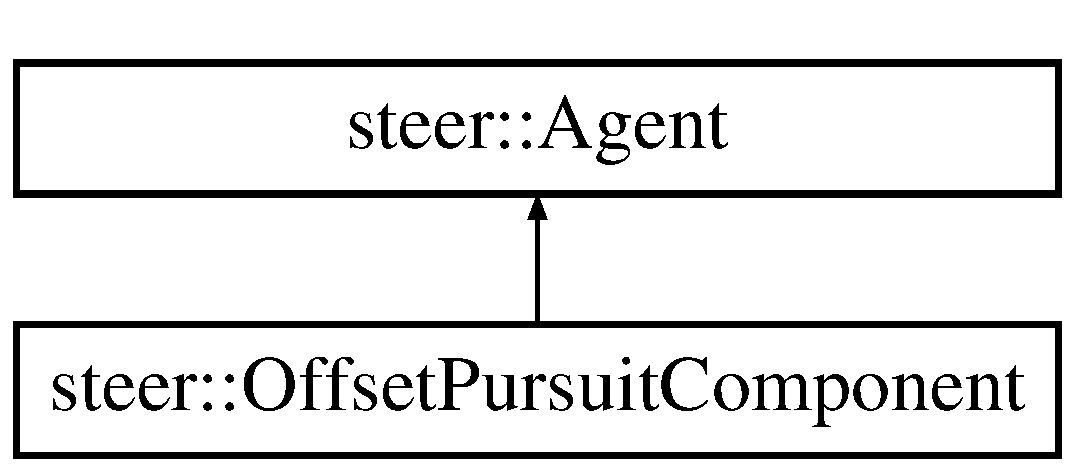
\includegraphics[height=2.000000cm]{classsteer_1_1_offset_pursuit_component}
\end{center}
\end{figure}
\subsection*{Public Member Functions}
\begin{DoxyCompactItemize}
\item 
\hypertarget{classsteer_1_1_offset_pursuit_component_aff55362cf15ea271b8563f7509a11ef5}{{\bfseries Offset\-Pursuit\-Component} (\hyperlink{structsteer_1_1_behavior_parameters}{steer\-::\-Behavior\-Parameters} $\ast$params)}\label{classsteer_1_1_offset_pursuit_component_aff55362cf15ea271b8563f7509a11ef5}

\item 
void \hyperlink{classsteer_1_1_offset_pursuit_component_afa17a1f914ea3f8c06e65c13ab6f4b21}{set\-Weight} (const float weight)
\begin{DoxyCompactList}\small\item\em Set the value of the weight multiplier for the Offset\-Pursuit component. \end{DoxyCompactList}\item 
\hypertarget{classsteer_1_1_offset_pursuit_component_a9d2e14e78dfbdc3ef6791aa2771dc126}{float \hyperlink{classsteer_1_1_offset_pursuit_component_a9d2e14e78dfbdc3ef6791aa2771dc126}{get\-Weight} () const }\label{classsteer_1_1_offset_pursuit_component_a9d2e14e78dfbdc3ef6791aa2771dc126}

\begin{DoxyCompactList}\small\item\em Get the value of the weight multiplier for the Offset\-Pursuit component. \end{DoxyCompactList}\item 
\hypertarget{classsteer_1_1_offset_pursuit_component_a24467edbaec6e36e8291669303ab3856}{void \hyperlink{classsteer_1_1_offset_pursuit_component_a24467edbaec6e36e8291669303ab3856}{set\-Rotation} (float r)}\label{classsteer_1_1_offset_pursuit_component_a24467edbaec6e36e8291669303ab3856}

\begin{DoxyCompactList}\small\item\em Set the value of the Offset\-Pursuit component rotation. \end{DoxyCompactList}\item 
\hypertarget{classsteer_1_1_offset_pursuit_component_a85cc7c083e1f6a4de0ffab4d49aa48a1}{float \hyperlink{classsteer_1_1_offset_pursuit_component_a85cc7c083e1f6a4de0ffab4d49aa48a1}{get\-Rotation} ()}\label{classsteer_1_1_offset_pursuit_component_a85cc7c083e1f6a4de0ffab4d49aa48a1}

\begin{DoxyCompactList}\small\item\em Get the value of the Offset\-Pursuit component rotation. \end{DoxyCompactList}\item 
virtual bool \hyperlink{classsteer_1_1_offset_pursuit_component_a748847de5cec80589b12b35214c5b5e2}{on} (\hyperlink{namespacesteer_afe6e72f8f8088962727051501181acbe}{steer\-::behavior\-Type} behavior)
\begin{DoxyCompactList}\small\item\em This pure virtual function tests if a specific bit of m\-\_\-i\-Flags is set using bitwise operations. Must be overridden in derived classes. \end{DoxyCompactList}\item 
\hypertarget{classsteer_1_1_offset_pursuit_component_ab00f431004a8582d9e92b1f5b866e960}{void {\bfseries Offset\-Pursuit\-On} ()}\label{classsteer_1_1_offset_pursuit_component_ab00f431004a8582d9e92b1f5b866e960}

\item 
\hypertarget{classsteer_1_1_offset_pursuit_component_aa637ba4d4f93d015dfa433325d18aaa4}{bool {\bfseries is\-Offset\-Pursuit\-On} ()}\label{classsteer_1_1_offset_pursuit_component_aa637ba4d4f93d015dfa433325d18aaa4}

\item 
\hypertarget{classsteer_1_1_offset_pursuit_component_af21028fac719260959481e2296e5a517}{void {\bfseries offset\-Pursuit\-Off} ()}\label{classsteer_1_1_offset_pursuit_component_af21028fac719260959481e2296e5a517}

\item 
\hypertarget{classsteer_1_1_offset_pursuit_component_a409340ab402b0c0b2df5861cc91f7749}{void {\bfseries set\-Leader} (\hyperlink{classsteer_1_1_agent}{steer\-::\-Agent} $\ast$l)}\label{classsteer_1_1_offset_pursuit_component_a409340ab402b0c0b2df5861cc91f7749}

\item 
\hypertarget{classsteer_1_1_offset_pursuit_component_a5bb14173697216a63b12edcc781b0625}{\hyperlink{classsteer_1_1_agent}{steer\-::\-Agent} $\ast$ {\bfseries get\-Leader} () const }\label{classsteer_1_1_offset_pursuit_component_a5bb14173697216a63b12edcc781b0625}

\item 
\hypertarget{classsteer_1_1_offset_pursuit_component_a7f1a09cd6bd639a433d997f2e87cc269}{virtual \hyperlink{structsteer_1_1_vector2}{Vector2} \hyperlink{classsteer_1_1_offset_pursuit_component_a7f1a09cd6bd639a433d997f2e87cc269}{Calculate} ()}\label{classsteer_1_1_offset_pursuit_component_a7f1a09cd6bd639a433d997f2e87cc269}

\begin{DoxyCompactList}\small\item\em A pure virtual method for calculating the steering vector. \end{DoxyCompactList}\item 
\hypertarget{classsteer_1_1_offset_pursuit_component_ab2734e526e86322deae566212982cb0e}{void {\bfseries Update} (float dt)}\label{classsteer_1_1_offset_pursuit_component_ab2734e526e86322deae566212982cb0e}

\end{DoxyCompactItemize}
\subsection*{Additional Inherited Members}


\subsection{Detailed Description}
An example implementation of the offset pursuit steering behavior. 

\subsection{Member Function Documentation}
\hypertarget{classsteer_1_1_offset_pursuit_component_a748847de5cec80589b12b35214c5b5e2}{\index{steer\-::\-Offset\-Pursuit\-Component@{steer\-::\-Offset\-Pursuit\-Component}!on@{on}}
\index{on@{on}!steer::OffsetPursuitComponent@{steer\-::\-Offset\-Pursuit\-Component}}
\subsubsection[{on}]{\setlength{\rightskip}{0pt plus 5cm}virtual bool steer\-::\-Offset\-Pursuit\-Component\-::on (
\begin{DoxyParamCaption}
\item[{{\bf steer\-::behavior\-Type}}]{behavior}
\end{DoxyParamCaption}
)\hspace{0.3cm}{\ttfamily [inline]}, {\ttfamily [virtual]}}}\label{classsteer_1_1_offset_pursuit_component_a748847de5cec80589b12b35214c5b5e2}


This pure virtual function tests if a specific bit of m\-\_\-i\-Flags is set using bitwise operations. Must be overridden in derived classes. 


\begin{DoxyParams}{Parameters}
{\em behavior} & -\/ enum behavior\-Type. \\
\hline
\end{DoxyParams}


Implements \hyperlink{classsteer_1_1_agent_a707204e49e6519c7a8ea0f3ded608d98}{steer\-::\-Agent}.

\hypertarget{classsteer_1_1_offset_pursuit_component_afa17a1f914ea3f8c06e65c13ab6f4b21}{\index{steer\-::\-Offset\-Pursuit\-Component@{steer\-::\-Offset\-Pursuit\-Component}!set\-Weight@{set\-Weight}}
\index{set\-Weight@{set\-Weight}!steer::OffsetPursuitComponent@{steer\-::\-Offset\-Pursuit\-Component}}
\subsubsection[{set\-Weight}]{\setlength{\rightskip}{0pt plus 5cm}void steer\-::\-Offset\-Pursuit\-Component\-::set\-Weight (
\begin{DoxyParamCaption}
\item[{const float}]{weight}
\end{DoxyParamCaption}
)\hspace{0.3cm}{\ttfamily [inline]}}}\label{classsteer_1_1_offset_pursuit_component_afa17a1f914ea3f8c06e65c13ab6f4b21}


Set the value of the weight multiplier for the Offset\-Pursuit component. 


\begin{DoxyParams}{Parameters}
{\em weight} & -\/ a plain old float. \\
\hline
\end{DoxyParams}


The documentation for this class was generated from the following files\-:\begin{DoxyCompactItemize}
\item 
include/steeriously/components/Offset\-Pursuit\-Component.\-hpp\item 
src/steeriously/components/Offset\-Pursuit\-Component.\-cpp\end{DoxyCompactItemize}

\hypertarget{classsteer_1_1_path}{\section{steer\-:\-:Path Class Reference}
\label{classsteer_1_1_path}\index{steer\-::\-Path@{steer\-::\-Path}}
}


Class providing the necessary structure for path following behavior.  




{\ttfamily \#include $<$Path.\-hpp$>$}

\subsection*{Public Member Functions}
\begin{DoxyCompactItemize}
\item 
\hypertarget{classsteer_1_1_path_a9ea093f9196ead3d5724509d7fc4d3e5}{\hyperlink{classsteer_1_1_path_a9ea093f9196ead3d5724509d7fc4d3e5}{Path} ()}\label{classsteer_1_1_path_a9ea093f9196ead3d5724509d7fc4d3e5}

\begin{DoxyCompactList}\small\item\em Default constructor. \end{DoxyCompactList}\item 
\hyperlink{classsteer_1_1_path_a36c4ed5fc8d2d3e4747920c0bedfbb97}{Path} (int Num\-Waypoints, std\-::list$<$ \hyperlink{structsteer_1_1_vector2}{steer\-::\-Vector2} $>$ \&waypoints)
\begin{DoxyCompactList}\small\item\em Constructor used for creating a path from a list of waypoints. \end{DoxyCompactList}\item 
\hyperlink{classsteer_1_1_path_a4c0811fa900426c5ee36d00c33af7ed5}{Path} (int Num\-Waypoints, float Min\-X, float Min\-Y, float Max\-X, float Max\-Y, bool looped)
\begin{DoxyCompactList}\small\item\em Constructor for creating a path with initial random waypoints. Min\-X/\-Y \& Max\-X/\-Y define the bounding box of the path. \end{DoxyCompactList}\item 
\hypertarget{classsteer_1_1_path_aaae6cb3aed1cd324e36ad61fd88221db}{\hyperlink{classsteer_1_1_path_aaae6cb3aed1cd324e36ad61fd88221db}{$\sim$\-Path} ()}\label{classsteer_1_1_path_aaae6cb3aed1cd324e36ad61fd88221db}

\begin{DoxyCompactList}\small\item\em Destructor. \end{DoxyCompactList}\item 
\hypertarget{classsteer_1_1_path_a29340827e82b14da98cc6e10e67bffa6}{\hyperlink{structsteer_1_1_vector2}{steer\-::\-Vector2} \hyperlink{classsteer_1_1_path_a29340827e82b14da98cc6e10e67bffa6}{current\-Waypoint} () const }\label{classsteer_1_1_path_a29340827e82b14da98cc6e10e67bffa6}

\begin{DoxyCompactList}\small\item\em Returns the current waypoint. \end{DoxyCompactList}\item 
\hypertarget{classsteer_1_1_path_af3bf9a7135709983607bccbc1c501c0d}{bool \hyperlink{classsteer_1_1_path_af3bf9a7135709983607bccbc1c501c0d}{finished} ()}\label{classsteer_1_1_path_af3bf9a7135709983607bccbc1c501c0d}

\begin{DoxyCompactList}\small\item\em Returns true if the end of the list has been reached. \end{DoxyCompactList}\item 
\hypertarget{classsteer_1_1_path_a54802e44fde08a217ac9b9ea1321b911}{void \hyperlink{classsteer_1_1_path_a54802e44fde08a217ac9b9ea1321b911}{set\-Next\-Waypoint} ()}\label{classsteer_1_1_path_a54802e44fde08a217ac9b9ea1321b911}

\begin{DoxyCompactList}\small\item\em Moves the iterator on to the next waypoint in the list. \end{DoxyCompactList}\item 
std\-::list$<$ \hyperlink{structsteer_1_1_vector2}{steer\-::\-Vector2} $>$ \hyperlink{classsteer_1_1_path_a6d1d4e9870f39dbec71dcda56044e0e7}{create\-Random\-Path} (int Num\-Waypoints, float Min\-X, float Min\-Y, float Max\-X, float Max\-Y)
\begin{DoxyCompactList}\small\item\em Creates a random path which is bound by rectangle described by the min/max values. \end{DoxyCompactList}\item 
\hypertarget{classsteer_1_1_path_a60efd7a0cc089e1dad6483dd3e378355}{void \hyperlink{classsteer_1_1_path_a60efd7a0cc089e1dad6483dd3e378355}{loop\-On} ()}\label{classsteer_1_1_path_a60efd7a0cc089e1dad6483dd3e378355}

\begin{DoxyCompactList}\small\item\em Turn on the loop option for the path so the path meets the first waypoint. \end{DoxyCompactList}\item 
\hypertarget{classsteer_1_1_path_a0f872c277f30488a9eed65acf3934093}{void \hyperlink{classsteer_1_1_path_a0f872c277f30488a9eed65acf3934093}{loop\-Off} ()}\label{classsteer_1_1_path_a0f872c277f30488a9eed65acf3934093}

\begin{DoxyCompactList}\small\item\em Turn off the loop option for the path so the path ends on the last waypoint. \end{DoxyCompactList}\item 
void \hyperlink{classsteer_1_1_path_abd66161db6441fad51d5cda43f7c0b13}{set} (std\-::list$<$ \hyperlink{structsteer_1_1_vector2}{steer\-::\-Vector2} $>$ new\-Path)
\begin{DoxyCompactList}\small\item\em Method for setting the path with list of vectors. \end{DoxyCompactList}\item 
void \hyperlink{classsteer_1_1_path_a9bf49c27d91fe8316a866d4483574a13}{set} (const \hyperlink{classsteer_1_1_path}{Path} \&path)
\begin{DoxyCompactList}\small\item\em Method for setting the path with a previously defined \hyperlink{classsteer_1_1_path}{Path}. \end{DoxyCompactList}\item 
\hypertarget{classsteer_1_1_path_a76d63db05197b28767e5fa13befb7dbe}{void \hyperlink{classsteer_1_1_path_a76d63db05197b28767e5fa13befb7dbe}{clear} ()}\label{classsteer_1_1_path_a76d63db05197b28767e5fa13befb7dbe}

\begin{DoxyCompactList}\small\item\em Clears all waypoints in the path std\-::vector. \end{DoxyCompactList}\item 
\hypertarget{classsteer_1_1_path_aedf4d447eb5286a3ff16562ee34c5bcd}{std\-::list$<$ \hyperlink{structsteer_1_1_vector2}{steer\-::\-Vector2} $>$ \hyperlink{classsteer_1_1_path_aedf4d447eb5286a3ff16562ee34c5bcd}{get\-Path} () const }\label{classsteer_1_1_path_aedf4d447eb5286a3ff16562ee34c5bcd}

\begin{DoxyCompactList}\small\item\em Returns the std\-::vector of waypoints in the path. \end{DoxyCompactList}\end{DoxyCompactItemize}


\subsection{Detailed Description}
Class providing the necessary structure for path following behavior. 

\subsection{Constructor \& Destructor Documentation}
\hypertarget{classsteer_1_1_path_a36c4ed5fc8d2d3e4747920c0bedfbb97}{\index{steer\-::\-Path@{steer\-::\-Path}!Path@{Path}}
\index{Path@{Path}!steer::Path@{steer\-::\-Path}}
\subsubsection[{Path}]{\setlength{\rightskip}{0pt plus 5cm}steer\-::\-Path\-::\-Path (
\begin{DoxyParamCaption}
\item[{int}]{Num\-Waypoints, }
\item[{std\-::list$<$ {\bf steer\-::\-Vector2} $>$ \&}]{waypoints}
\end{DoxyParamCaption}
)}}\label{classsteer_1_1_path_a36c4ed5fc8d2d3e4747920c0bedfbb97}


Constructor used for creating a path from a list of waypoints. 


\begin{DoxyParams}{Parameters}
{\em Num\-Waypoints} & -\/ a plain old int. \\
\hline
{\em waypoints} & -\/ a std\-::list of \hyperlink{structsteer_1_1_vector2}{steer\-::\-Vector2}. \\
\hline
\end{DoxyParams}
\hypertarget{classsteer_1_1_path_a4c0811fa900426c5ee36d00c33af7ed5}{\index{steer\-::\-Path@{steer\-::\-Path}!Path@{Path}}
\index{Path@{Path}!steer::Path@{steer\-::\-Path}}
\subsubsection[{Path}]{\setlength{\rightskip}{0pt plus 5cm}steer\-::\-Path\-::\-Path (
\begin{DoxyParamCaption}
\item[{int}]{Num\-Waypoints, }
\item[{float}]{Min\-X, }
\item[{float}]{Min\-Y, }
\item[{float}]{Max\-X, }
\item[{float}]{Max\-Y, }
\item[{bool}]{looped}
\end{DoxyParamCaption}
)}}\label{classsteer_1_1_path_a4c0811fa900426c5ee36d00c33af7ed5}


Constructor for creating a path with initial random waypoints. Min\-X/\-Y \& Max\-X/\-Y define the bounding box of the path. 


\begin{DoxyParams}{Parameters}
{\em Num\-Waypoints} & -\/ a plain old int. \\
\hline
{\em Min\-X} & -\/ a plain old float. \\
\hline
{\em Min\-Y} & -\/ a plain old float. \\
\hline
{\em Max\-X} & -\/ a plain old float. \\
\hline
{\em Max\-Y} & -\/ a plain old float. \\
\hline
{\em looped} & -\/ a plain old bool. \\
\hline
\end{DoxyParams}


\subsection{Member Function Documentation}
\hypertarget{classsteer_1_1_path_a6d1d4e9870f39dbec71dcda56044e0e7}{\index{steer\-::\-Path@{steer\-::\-Path}!create\-Random\-Path@{create\-Random\-Path}}
\index{create\-Random\-Path@{create\-Random\-Path}!steer::Path@{steer\-::\-Path}}
\subsubsection[{create\-Random\-Path}]{\setlength{\rightskip}{0pt plus 5cm}std\-::list$<$ {\bf Vector2} $>$ steer\-::\-Path\-::create\-Random\-Path (
\begin{DoxyParamCaption}
\item[{int}]{Num\-Waypoints, }
\item[{float}]{Min\-X, }
\item[{float}]{Min\-Y, }
\item[{float}]{Max\-X, }
\item[{float}]{Max\-Y}
\end{DoxyParamCaption}
)}}\label{classsteer_1_1_path_a6d1d4e9870f39dbec71dcda56044e0e7}


Creates a random path which is bound by rectangle described by the min/max values. 


\begin{DoxyParams}{Parameters}
{\em Num\-Waypoints} & -\/ a plain old int. \\
\hline
{\em Min\-X} & -\/ a plain old float. \\
\hline
{\em Min\-Y} & -\/ a plain old float. \\
\hline
{\em Max\-X} & -\/ a plain old float. \\
\hline
{\em Max\-Y} & -\/ a plain old float. \\
\hline
\end{DoxyParams}
\hypertarget{classsteer_1_1_path_abd66161db6441fad51d5cda43f7c0b13}{\index{steer\-::\-Path@{steer\-::\-Path}!set@{set}}
\index{set@{set}!steer::Path@{steer\-::\-Path}}
\subsubsection[{set}]{\setlength{\rightskip}{0pt plus 5cm}void steer\-::\-Path\-::set (
\begin{DoxyParamCaption}
\item[{std\-::list$<$ {\bf steer\-::\-Vector2} $>$}]{new\-Path}
\end{DoxyParamCaption}
)\hspace{0.3cm}{\ttfamily [inline]}}}\label{classsteer_1_1_path_abd66161db6441fad51d5cda43f7c0b13}


Method for setting the path with list of vectors. 


\begin{DoxyParams}{Parameters}
{\em new\-Path} & -\/ a std\-::vector of \hyperlink{structsteer_1_1_vector2}{steer\-::\-Vector2} floats. \\
\hline
\end{DoxyParams}
\hypertarget{classsteer_1_1_path_a9bf49c27d91fe8316a866d4483574a13}{\index{steer\-::\-Path@{steer\-::\-Path}!set@{set}}
\index{set@{set}!steer::Path@{steer\-::\-Path}}
\subsubsection[{set}]{\setlength{\rightskip}{0pt plus 5cm}steer\-::\-Path\-::set (
\begin{DoxyParamCaption}
\item[{const {\bf Path} \&}]{path}
\end{DoxyParamCaption}
)\hspace{0.3cm}{\ttfamily [inline]}}}\label{classsteer_1_1_path_a9bf49c27d91fe8316a866d4483574a13}


Method for setting the path with a previously defined \hyperlink{classsteer_1_1_path}{Path}. 


\begin{DoxyParams}{Parameters}
{\em path} & -\/ a \hyperlink{classsteer_1_1_path}{steer\-::\-Path} object. \\
\hline
\end{DoxyParams}


The documentation for this class was generated from the following files\-:\begin{DoxyCompactItemize}
\item 
include/steeriously/Path.\-hpp\item 
src/steeriously/Path.\-cpp\end{DoxyCompactItemize}

\hypertarget{classsteer_1_1_path_following_component}{\section{steer\-:\-:Path\-Following\-Component Class Reference}
\label{classsteer_1_1_path_following_component}\index{steer\-::\-Path\-Following\-Component@{steer\-::\-Path\-Following\-Component}}
}


An example implementation of the path following steering behavior.  




{\ttfamily \#include $<$Path\-Following\-Component.\-hpp$>$}

Inheritance diagram for steer\-:\-:Path\-Following\-Component\-:\begin{figure}[H]
\begin{center}
\leavevmode
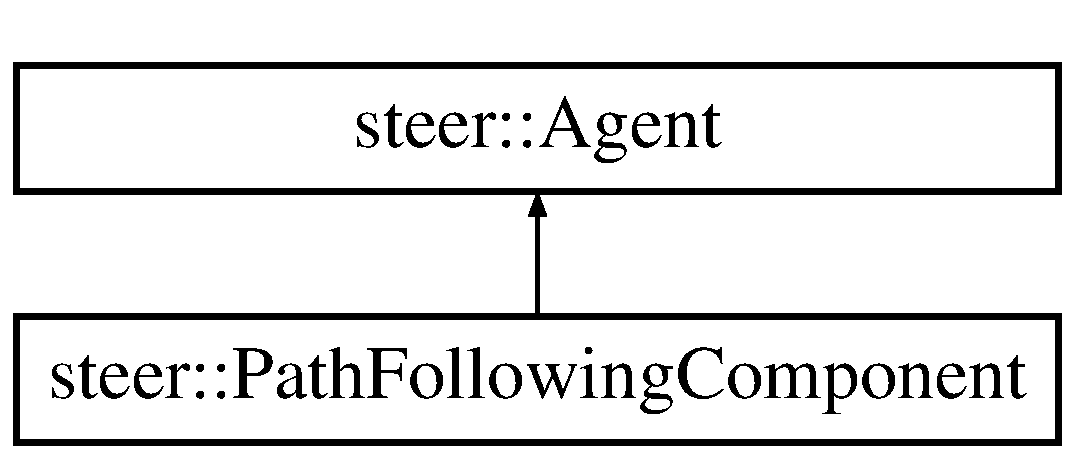
\includegraphics[height=2.000000cm]{classsteer_1_1_path_following_component}
\end{center}
\end{figure}
\subsection*{Public Member Functions}
\begin{DoxyCompactItemize}
\item 
\hypertarget{classsteer_1_1_path_following_component_a5d874cbfb0538b9766c8539ec225524d}{{\bfseries Path\-Following\-Component} (\hyperlink{structsteer_1_1_behavior_parameters}{steer\-::\-Behavior\-Parameters} $\ast$params)}\label{classsteer_1_1_path_following_component_a5d874cbfb0538b9766c8539ec225524d}

\item 
\hypertarget{classsteer_1_1_path_following_component_a5cd103a2bd79b1f2b4ff39531534dce3}{{\bfseries Path\-Following\-Component} (\hyperlink{classsteer_1_1_path}{steer\-::\-Path} $\ast$p, \hyperlink{structsteer_1_1_behavior_parameters}{steer\-::\-Behavior\-Parameters} $\ast$params)}\label{classsteer_1_1_path_following_component_a5cd103a2bd79b1f2b4ff39531534dce3}

\item 
void \hyperlink{classsteer_1_1_path_following_component_a74524118217244adfb1d572706d2e357}{set\-Weight} (const float weight)
\begin{DoxyCompactList}\small\item\em Set the value of the weight multiplier for the \hyperlink{classsteer_1_1_path}{Path} Following component. \end{DoxyCompactList}\item 
\hypertarget{classsteer_1_1_path_following_component_ae6081f8fa8f25f01cacd778bcae3f085}{float \hyperlink{classsteer_1_1_path_following_component_ae6081f8fa8f25f01cacd778bcae3f085}{get\-Weight} () const }\label{classsteer_1_1_path_following_component_ae6081f8fa8f25f01cacd778bcae3f085}

\begin{DoxyCompactList}\small\item\em Get the value of the weight multiplier for the \hyperlink{classsteer_1_1_path}{Path} Following component. \end{DoxyCompactList}\item 
\hypertarget{classsteer_1_1_path_following_component_a3b6b6a7a99853dfe9579b0022962239a}{void \hyperlink{classsteer_1_1_path_following_component_a3b6b6a7a99853dfe9579b0022962239a}{set\-Rotation} (float r)}\label{classsteer_1_1_path_following_component_a3b6b6a7a99853dfe9579b0022962239a}

\begin{DoxyCompactList}\small\item\em Set the value of the \hyperlink{classsteer_1_1_path}{Path} Following component rotation. \end{DoxyCompactList}\item 
\hypertarget{classsteer_1_1_path_following_component_a5e40a561950d6b723b044472260bd2b8}{float \hyperlink{classsteer_1_1_path_following_component_a5e40a561950d6b723b044472260bd2b8}{get\-Rotation} ()}\label{classsteer_1_1_path_following_component_a5e40a561950d6b723b044472260bd2b8}

\begin{DoxyCompactList}\small\item\em Get the value of the \hyperlink{classsteer_1_1_path}{Path} Following component rotation. \end{DoxyCompactList}\item 
\hypertarget{classsteer_1_1_path_following_component_a7059cf601823298f88be089b9b066d39}{void {\bfseries set\-Path} (\hyperlink{classsteer_1_1_path}{steer\-::\-Path} $\ast$p)}\label{classsteer_1_1_path_following_component_a7059cf601823298f88be089b9b066d39}

\item 
\hypertarget{classsteer_1_1_path_following_component_a6bc0a5a3aeac0df2f4d1bf2782834b4d}{\hyperlink{classsteer_1_1_path}{steer\-::\-Path} $\ast$ {\bfseries get\-Path} () const }\label{classsteer_1_1_path_following_component_a6bc0a5a3aeac0df2f4d1bf2782834b4d}

\item 
virtual bool \hyperlink{classsteer_1_1_path_following_component_af15d403db80ac9d623d6fc4ec6f6701b}{on} (\hyperlink{namespacesteer_afe6e72f8f8088962727051501181acbe}{steer\-::behavior\-Type} behavior)
\begin{DoxyCompactList}\small\item\em This pure virtual function tests if a specific bit of m\-\_\-i\-Flags is set using bitwise operations. Must be overridden in derived classes. \end{DoxyCompactList}\item 
\hypertarget{classsteer_1_1_path_following_component_a7b795c82dd889c9b15965486b41f1dee}{void {\bfseries path\-Following\-On} ()}\label{classsteer_1_1_path_following_component_a7b795c82dd889c9b15965486b41f1dee}

\item 
\hypertarget{classsteer_1_1_path_following_component_a19cf5261b9483f2a8ec8fe83328bd516}{bool {\bfseries is\-Path\-Following\-On} ()}\label{classsteer_1_1_path_following_component_a19cf5261b9483f2a8ec8fe83328bd516}

\item 
\hypertarget{classsteer_1_1_path_following_component_a36b3fdf6732f58cdb96159cd47acc7f8}{void {\bfseries path\-Following\-Off} ()}\label{classsteer_1_1_path_following_component_a36b3fdf6732f58cdb96159cd47acc7f8}

\item 
\hypertarget{classsteer_1_1_path_following_component_a196c16619b471663b4a53e39def2cdca}{bool {\bfseries target\-Acquired} ()}\label{classsteer_1_1_path_following_component_a196c16619b471663b4a53e39def2cdca}

\item 
\hypertarget{classsteer_1_1_path_following_component_a5f7f64ffa13cb224df7732239df1de1d}{virtual \hyperlink{structsteer_1_1_vector2}{Vector2} \hyperlink{classsteer_1_1_path_following_component_a5f7f64ffa13cb224df7732239df1de1d}{Calculate} ()}\label{classsteer_1_1_path_following_component_a5f7f64ffa13cb224df7732239df1de1d}

\begin{DoxyCompactList}\small\item\em A pure virtual method for calculating the steering vector. \end{DoxyCompactList}\item 
\hypertarget{classsteer_1_1_path_following_component_af35b96d85c2a900296b0fc7b0f2036b6}{void {\bfseries Update} (float dt)}\label{classsteer_1_1_path_following_component_af35b96d85c2a900296b0fc7b0f2036b6}

\end{DoxyCompactItemize}
\subsection*{Additional Inherited Members}


\subsection{Detailed Description}
An example implementation of the path following steering behavior. 

\subsection{Member Function Documentation}
\hypertarget{classsteer_1_1_path_following_component_af15d403db80ac9d623d6fc4ec6f6701b}{\index{steer\-::\-Path\-Following\-Component@{steer\-::\-Path\-Following\-Component}!on@{on}}
\index{on@{on}!steer::PathFollowingComponent@{steer\-::\-Path\-Following\-Component}}
\subsubsection[{on}]{\setlength{\rightskip}{0pt plus 5cm}virtual bool steer\-::\-Path\-Following\-Component\-::on (
\begin{DoxyParamCaption}
\item[{{\bf steer\-::behavior\-Type}}]{behavior}
\end{DoxyParamCaption}
)\hspace{0.3cm}{\ttfamily [inline]}, {\ttfamily [virtual]}}}\label{classsteer_1_1_path_following_component_af15d403db80ac9d623d6fc4ec6f6701b}


This pure virtual function tests if a specific bit of m\-\_\-i\-Flags is set using bitwise operations. Must be overridden in derived classes. 


\begin{DoxyParams}{Parameters}
{\em behavior} & -\/ enum behavior\-Type. \\
\hline
\end{DoxyParams}


Implements \hyperlink{classsteer_1_1_agent_a707204e49e6519c7a8ea0f3ded608d98}{steer\-::\-Agent}.

\hypertarget{classsteer_1_1_path_following_component_a74524118217244adfb1d572706d2e357}{\index{steer\-::\-Path\-Following\-Component@{steer\-::\-Path\-Following\-Component}!set\-Weight@{set\-Weight}}
\index{set\-Weight@{set\-Weight}!steer::PathFollowingComponent@{steer\-::\-Path\-Following\-Component}}
\subsubsection[{set\-Weight}]{\setlength{\rightskip}{0pt plus 5cm}void steer\-::\-Path\-Following\-Component\-::set\-Weight (
\begin{DoxyParamCaption}
\item[{const float}]{weight}
\end{DoxyParamCaption}
)\hspace{0.3cm}{\ttfamily [inline]}}}\label{classsteer_1_1_path_following_component_a74524118217244adfb1d572706d2e357}


Set the value of the weight multiplier for the \hyperlink{classsteer_1_1_path}{Path} Following component. 


\begin{DoxyParams}{Parameters}
{\em weight} & -\/ a plain old float. \\
\hline
\end{DoxyParams}


The documentation for this class was generated from the following files\-:\begin{DoxyCompactItemize}
\item 
include/steeriously/components/Path\-Following\-Component.\-hpp\item 
src/steeriously/components/Path\-Following\-Component.\-cpp\end{DoxyCompactItemize}

\hypertarget{classsteer_1_1_pursuit_component}{\section{steer\-:\-:Pursuit\-Component Class Reference}
\label{classsteer_1_1_pursuit_component}\index{steer\-::\-Pursuit\-Component@{steer\-::\-Pursuit\-Component}}
}


An example implementation of the pursuit steering behavior.  




{\ttfamily \#include $<$Pursuit\-Component.\-hpp$>$}

Inheritance diagram for steer\-:\-:Pursuit\-Component\-:\begin{figure}[H]
\begin{center}
\leavevmode
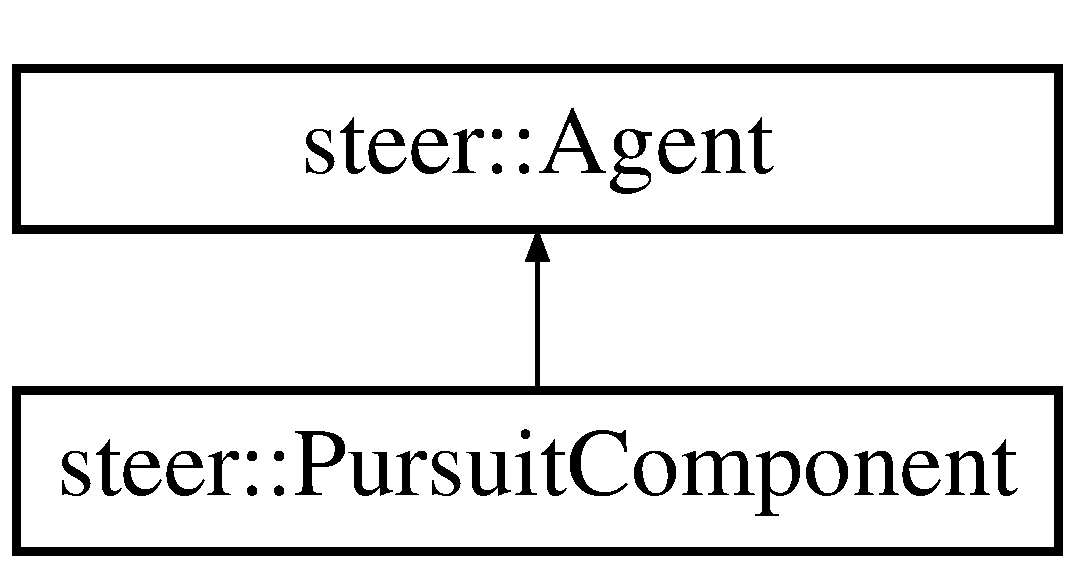
\includegraphics[height=2.000000cm]{classsteer_1_1_pursuit_component}
\end{center}
\end{figure}
\subsection*{Public Member Functions}
\begin{DoxyCompactItemize}
\item 
\hypertarget{classsteer_1_1_pursuit_component_a0042fb61e8bdad810446a3d59ac495c4}{{\bfseries Pursuit\-Component} (\hyperlink{structsteer_1_1_behavior_parameters}{steer\-::\-Behavior\-Parameters} $\ast$params)}\label{classsteer_1_1_pursuit_component_a0042fb61e8bdad810446a3d59ac495c4}

\item 
void \hyperlink{classsteer_1_1_pursuit_component_a23cb54c3718028ec7859f4350fe6dda1}{set\-Weight} (const float weight)
\begin{DoxyCompactList}\small\item\em Set the value of the weight multiplier for the Pursuit component. \end{DoxyCompactList}\item 
\hypertarget{classsteer_1_1_pursuit_component_ae361d87e084ece53b270267081e423e0}{float \hyperlink{classsteer_1_1_pursuit_component_ae361d87e084ece53b270267081e423e0}{get\-Weight} () const }\label{classsteer_1_1_pursuit_component_ae361d87e084ece53b270267081e423e0}

\begin{DoxyCompactList}\small\item\em Get the value of the weight multiplier for the Pursuit component. \end{DoxyCompactList}\item 
\hypertarget{classsteer_1_1_pursuit_component_a0098d8e1f606fd40377c8bcf581efd39}{void \hyperlink{classsteer_1_1_pursuit_component_a0098d8e1f606fd40377c8bcf581efd39}{set\-Rotation} (float r)}\label{classsteer_1_1_pursuit_component_a0098d8e1f606fd40377c8bcf581efd39}

\begin{DoxyCompactList}\small\item\em Set the value of the Pursuit component rotation. \end{DoxyCompactList}\item 
\hypertarget{classsteer_1_1_pursuit_component_ac2837285625673fc9df2a5af2c7a4457}{float \hyperlink{classsteer_1_1_pursuit_component_ac2837285625673fc9df2a5af2c7a4457}{get\-Rotation} ()}\label{classsteer_1_1_pursuit_component_ac2837285625673fc9df2a5af2c7a4457}

\begin{DoxyCompactList}\small\item\em Get the value of the Pursuit component rotation. \end{DoxyCompactList}\item 
virtual bool \hyperlink{classsteer_1_1_pursuit_component_a10e4d08aaca8aaf3d7041e281af2a519}{on} (\hyperlink{namespacesteer_afe6e72f8f8088962727051501181acbe}{steer\-::behavior\-Type} behavior)
\begin{DoxyCompactList}\small\item\em This pure virtual function tests if a specific bit of m\-\_\-i\-Flags is set using bitwise operations. Must be overridden in derived classes. \end{DoxyCompactList}\item 
\hypertarget{classsteer_1_1_pursuit_component_a02a94c1423b71b2c0dc017a42f9b9dff}{void {\bfseries pursuit\-On} ()}\label{classsteer_1_1_pursuit_component_a02a94c1423b71b2c0dc017a42f9b9dff}

\item 
\hypertarget{classsteer_1_1_pursuit_component_ae116f09357ae520ae625b8bdfb465167}{bool {\bfseries is\-Pursuit\-On} ()}\label{classsteer_1_1_pursuit_component_ae116f09357ae520ae625b8bdfb465167}

\item 
\hypertarget{classsteer_1_1_pursuit_component_a2046b1952c056a46287f7f7982d115e8}{void {\bfseries pursuit\-Off} ()}\label{classsteer_1_1_pursuit_component_a2046b1952c056a46287f7f7982d115e8}

\item 
\hypertarget{classsteer_1_1_pursuit_component_a6c1246c5310b182fcb033940dbb2c9ff}{void {\bfseries set\-Target\-Agent} (\hyperlink{classsteer_1_1_agent}{steer\-::\-Agent} $\ast$a)}\label{classsteer_1_1_pursuit_component_a6c1246c5310b182fcb033940dbb2c9ff}

\item 
\hypertarget{classsteer_1_1_pursuit_component_af9a95fbf5c379e32fdcff933d32def99}{\hyperlink{classsteer_1_1_agent}{steer\-::\-Agent} $\ast$ {\bfseries get\-Target\-Agent} () const }\label{classsteer_1_1_pursuit_component_af9a95fbf5c379e32fdcff933d32def99}

\item 
\hypertarget{classsteer_1_1_pursuit_component_ab0d9dca749f1a2474264b01badfd5fa2}{bool {\bfseries target\-Acquired} ()}\label{classsteer_1_1_pursuit_component_ab0d9dca749f1a2474264b01badfd5fa2}

\item 
\hypertarget{classsteer_1_1_pursuit_component_a644fa669d584d925b4c888bf67119045}{virtual \hyperlink{structsteer_1_1_vector2}{Vector2} \hyperlink{classsteer_1_1_pursuit_component_a644fa669d584d925b4c888bf67119045}{Calculate} ()}\label{classsteer_1_1_pursuit_component_a644fa669d584d925b4c888bf67119045}

\begin{DoxyCompactList}\small\item\em A pure virtual method for calculating the steering vector. \end{DoxyCompactList}\item 
\hypertarget{classsteer_1_1_pursuit_component_affa6ee80c32666ae2aca6e2536ccf261}{void {\bfseries Update} (float dt)}\label{classsteer_1_1_pursuit_component_affa6ee80c32666ae2aca6e2536ccf261}

\end{DoxyCompactItemize}
\subsection*{Additional Inherited Members}


\subsection{Detailed Description}
An example implementation of the pursuit steering behavior. 

\subsection{Member Function Documentation}
\hypertarget{classsteer_1_1_pursuit_component_a10e4d08aaca8aaf3d7041e281af2a519}{\index{steer\-::\-Pursuit\-Component@{steer\-::\-Pursuit\-Component}!on@{on}}
\index{on@{on}!steer::PursuitComponent@{steer\-::\-Pursuit\-Component}}
\subsubsection[{on}]{\setlength{\rightskip}{0pt plus 5cm}virtual bool steer\-::\-Pursuit\-Component\-::on (
\begin{DoxyParamCaption}
\item[{{\bf steer\-::behavior\-Type}}]{behavior}
\end{DoxyParamCaption}
)\hspace{0.3cm}{\ttfamily [inline]}, {\ttfamily [virtual]}}}\label{classsteer_1_1_pursuit_component_a10e4d08aaca8aaf3d7041e281af2a519}


This pure virtual function tests if a specific bit of m\-\_\-i\-Flags is set using bitwise operations. Must be overridden in derived classes. 


\begin{DoxyParams}{Parameters}
{\em behavior} & -\/ enum behavior\-Type. \\
\hline
\end{DoxyParams}


Implements \hyperlink{classsteer_1_1_agent_a707204e49e6519c7a8ea0f3ded608d98}{steer\-::\-Agent}.

\hypertarget{classsteer_1_1_pursuit_component_a23cb54c3718028ec7859f4350fe6dda1}{\index{steer\-::\-Pursuit\-Component@{steer\-::\-Pursuit\-Component}!set\-Weight@{set\-Weight}}
\index{set\-Weight@{set\-Weight}!steer::PursuitComponent@{steer\-::\-Pursuit\-Component}}
\subsubsection[{set\-Weight}]{\setlength{\rightskip}{0pt plus 5cm}void steer\-::\-Pursuit\-Component\-::set\-Weight (
\begin{DoxyParamCaption}
\item[{const float}]{weight}
\end{DoxyParamCaption}
)\hspace{0.3cm}{\ttfamily [inline]}}}\label{classsteer_1_1_pursuit_component_a23cb54c3718028ec7859f4350fe6dda1}


Set the value of the weight multiplier for the Pursuit component. 


\begin{DoxyParams}{Parameters}
{\em weight} & -\/ a plain old float. \\
\hline
\end{DoxyParams}


The documentation for this class was generated from the following files\-:\begin{DoxyCompactItemize}
\item 
include/steeriously/components/Pursuit\-Component.\-hpp\item 
src/steeriously/components/Pursuit\-Component.\-cpp\end{DoxyCompactItemize}

\hypertarget{classsteer_1_1_seek_component}{\section{steer\-:\-:Seek\-Component Class Reference}
\label{classsteer_1_1_seek_component}\index{steer\-::\-Seek\-Component@{steer\-::\-Seek\-Component}}
}


An example implementation of the seek steering behavior.  




{\ttfamily \#include $<$Seek\-Component.\-hpp$>$}

Inheritance diagram for steer\-:\-:Seek\-Component\-:\begin{figure}[H]
\begin{center}
\leavevmode
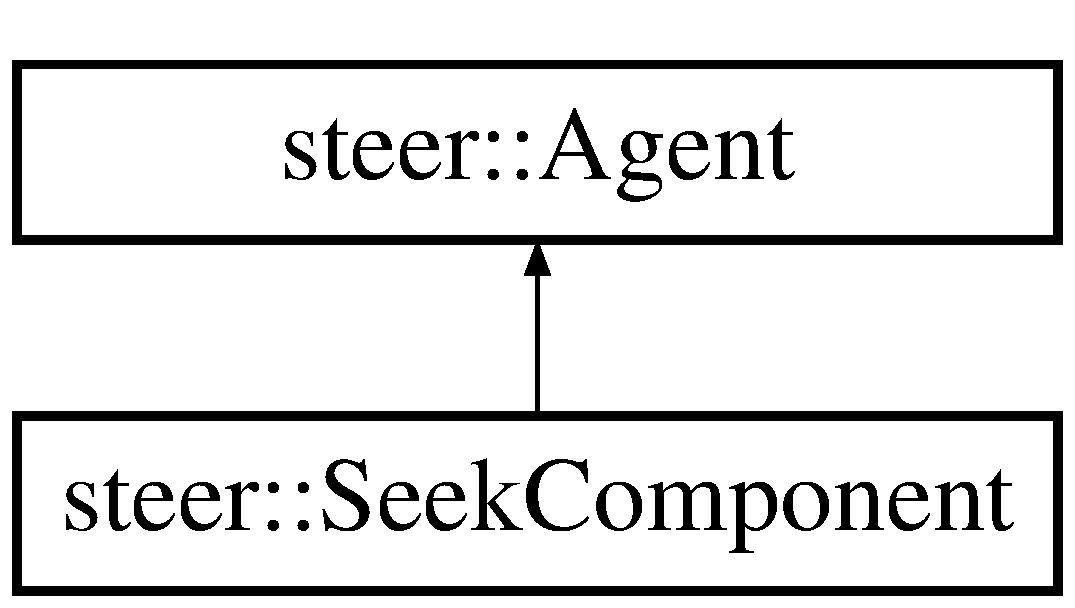
\includegraphics[height=2.000000cm]{classsteer_1_1_seek_component}
\end{center}
\end{figure}
\subsection*{Public Member Functions}
\begin{DoxyCompactItemize}
\item 
\hypertarget{classsteer_1_1_seek_component_af7664e661c7ac568ca0ee97a84fcdd84}{{\bfseries Seek\-Component} (\hyperlink{structsteer_1_1_behavior_parameters}{steer\-::\-Behavior\-Parameters} $\ast$params)}\label{classsteer_1_1_seek_component_af7664e661c7ac568ca0ee97a84fcdd84}

\item 
void \hyperlink{classsteer_1_1_seek_component_ab581d425507b79abf04b227528f31f14}{set\-Weight} (const float weight)
\begin{DoxyCompactList}\small\item\em Set the value of the weight multiplier for the seek component. \end{DoxyCompactList}\item 
\hypertarget{classsteer_1_1_seek_component_a67c969244ed054dfb5a6abab6711b052}{float \hyperlink{classsteer_1_1_seek_component_a67c969244ed054dfb5a6abab6711b052}{get\-Weight} () const }\label{classsteer_1_1_seek_component_a67c969244ed054dfb5a6abab6711b052}

\begin{DoxyCompactList}\small\item\em Get the value of the weight multiplier for the seek component. \end{DoxyCompactList}\item 
\hypertarget{classsteer_1_1_seek_component_a7ecf69c4146448c36d626b89c430eaff}{void \hyperlink{classsteer_1_1_seek_component_a7ecf69c4146448c36d626b89c430eaff}{set\-Rotation} (float r)}\label{classsteer_1_1_seek_component_a7ecf69c4146448c36d626b89c430eaff}

\begin{DoxyCompactList}\small\item\em Set the value of the seek component rotation. \end{DoxyCompactList}\item 
\hypertarget{classsteer_1_1_seek_component_a391b89cc1e8d54061f81dca5ab852c89}{float \hyperlink{classsteer_1_1_seek_component_a391b89cc1e8d54061f81dca5ab852c89}{get\-Rotation} ()}\label{classsteer_1_1_seek_component_a391b89cc1e8d54061f81dca5ab852c89}

\begin{DoxyCompactList}\small\item\em Get the value of the seek component rotation. \end{DoxyCompactList}\item 
virtual bool \hyperlink{classsteer_1_1_seek_component_a02782af7638a7dfc59de647ba810d0ae}{on} (\hyperlink{namespacesteer_afe6e72f8f8088962727051501181acbe}{steer\-::behavior\-Type} behavior)
\begin{DoxyCompactList}\small\item\em This pure virtual function tests if a specific bit of m\-\_\-i\-Flags is set using bitwise operations. Must be overridden in derived classes. \end{DoxyCompactList}\item 
\hypertarget{classsteer_1_1_seek_component_a93ff3518a3f6889ff98a8eb986098b8d}{void {\bfseries seek\-On} ()}\label{classsteer_1_1_seek_component_a93ff3518a3f6889ff98a8eb986098b8d}

\item 
\hypertarget{classsteer_1_1_seek_component_ad219116f6dd2b4edbedb613e510c85a7}{bool {\bfseries is\-Seek\-On} ()}\label{classsteer_1_1_seek_component_ad219116f6dd2b4edbedb613e510c85a7}

\item 
\hypertarget{classsteer_1_1_seek_component_a3d8d434aad5cc50f447a014a11bd74f3}{void {\bfseries seek\-Off} ()}\label{classsteer_1_1_seek_component_a3d8d434aad5cc50f447a014a11bd74f3}

\item 
\hypertarget{classsteer_1_1_seek_component_ac8c43fcaec1220eb23123563787411c0}{bool {\bfseries target\-Acquired} ()}\label{classsteer_1_1_seek_component_ac8c43fcaec1220eb23123563787411c0}

\item 
\hypertarget{classsteer_1_1_seek_component_afdf0d958f5b51deb07ec1e6c9c30fb6b}{virtual \hyperlink{structsteer_1_1_vector2}{Vector2} \hyperlink{classsteer_1_1_seek_component_afdf0d958f5b51deb07ec1e6c9c30fb6b}{Calculate} ()}\label{classsteer_1_1_seek_component_afdf0d958f5b51deb07ec1e6c9c30fb6b}

\begin{DoxyCompactList}\small\item\em A pure virtual method for calculating the steering vector. \end{DoxyCompactList}\item 
\hypertarget{classsteer_1_1_seek_component_a1121c7588fd4071fbf08bbe4164d3a23}{void {\bfseries Update} (float dt)}\label{classsteer_1_1_seek_component_a1121c7588fd4071fbf08bbe4164d3a23}

\end{DoxyCompactItemize}
\subsection*{Additional Inherited Members}


\subsection{Detailed Description}
An example implementation of the seek steering behavior. 

\subsection{Member Function Documentation}
\hypertarget{classsteer_1_1_seek_component_a02782af7638a7dfc59de647ba810d0ae}{\index{steer\-::\-Seek\-Component@{steer\-::\-Seek\-Component}!on@{on}}
\index{on@{on}!steer::SeekComponent@{steer\-::\-Seek\-Component}}
\subsubsection[{on}]{\setlength{\rightskip}{0pt plus 5cm}virtual bool steer\-::\-Seek\-Component\-::on (
\begin{DoxyParamCaption}
\item[{{\bf steer\-::behavior\-Type}}]{behavior}
\end{DoxyParamCaption}
)\hspace{0.3cm}{\ttfamily [inline]}, {\ttfamily [virtual]}}}\label{classsteer_1_1_seek_component_a02782af7638a7dfc59de647ba810d0ae}


This pure virtual function tests if a specific bit of m\-\_\-i\-Flags is set using bitwise operations. Must be overridden in derived classes. 


\begin{DoxyParams}{Parameters}
{\em behavior} & -\/ enum behavior\-Type. \\
\hline
\end{DoxyParams}


Implements \hyperlink{classsteer_1_1_agent_a707204e49e6519c7a8ea0f3ded608d98}{steer\-::\-Agent}.

\hypertarget{classsteer_1_1_seek_component_ab581d425507b79abf04b227528f31f14}{\index{steer\-::\-Seek\-Component@{steer\-::\-Seek\-Component}!set\-Weight@{set\-Weight}}
\index{set\-Weight@{set\-Weight}!steer::SeekComponent@{steer\-::\-Seek\-Component}}
\subsubsection[{set\-Weight}]{\setlength{\rightskip}{0pt plus 5cm}void steer\-::\-Seek\-Component\-::set\-Weight (
\begin{DoxyParamCaption}
\item[{const float}]{weight}
\end{DoxyParamCaption}
)\hspace{0.3cm}{\ttfamily [inline]}}}\label{classsteer_1_1_seek_component_ab581d425507b79abf04b227528f31f14}


Set the value of the weight multiplier for the seek component. 


\begin{DoxyParams}{Parameters}
{\em weight} & -\/ a plain old float. \\
\hline
\end{DoxyParams}


The documentation for this class was generated from the following files\-:\begin{DoxyCompactItemize}
\item 
include/steeriously/components/Seek\-Component.\-hpp\item 
src/steeriously/components/Seek\-Component.\-cpp\end{DoxyCompactItemize}

\hypertarget{classsteer_1_1_sphere_obstacle}{\section{steer\-:\-:Sphere\-Obstacle Class Reference}
\label{classsteer_1_1_sphere_obstacle}\index{steer\-::\-Sphere\-Obstacle@{steer\-::\-Sphere\-Obstacle}}
}


Class to aid in obstacle avoidance routine.  




{\ttfamily \#include $<$Sphere\-Obstacle.\-hpp$>$}

\subsection*{Public Member Functions}
\begin{DoxyCompactItemize}
\item 
\hyperlink{classsteer_1_1_sphere_obstacle_a7afc66c47d05366c1df420f54281fc5d}{Sphere\-Obstacle} (\hyperlink{structsteer_1_1_vector2}{steer\-::\-Vector2} position, float radius)
\begin{DoxyCompactList}\small\item\em Construct a sphere obstacle from a position and radius. \end{DoxyCompactList}\item 
\hypertarget{classsteer_1_1_sphere_obstacle_a5ca5b6c0047ffb7ded454c517656c688}{virtual \hyperlink{classsteer_1_1_sphere_obstacle_a5ca5b6c0047ffb7ded454c517656c688}{$\sim$\-Sphere\-Obstacle} ()}\label{classsteer_1_1_sphere_obstacle_a5ca5b6c0047ffb7ded454c517656c688}

\begin{DoxyCompactList}\small\item\em Destructor. \end{DoxyCompactList}\item 
\hypertarget{classsteer_1_1_sphere_obstacle_a707db36f3d4be339ac84b541144b9e6f}{bool \hyperlink{classsteer_1_1_sphere_obstacle_a707db36f3d4be339ac84b541144b9e6f}{tagged\-In\-Group} () const }\label{classsteer_1_1_sphere_obstacle_a707db36f3d4be339ac84b541144b9e6f}

\begin{DoxyCompactList}\small\item\em Gets the tag status of the obstacle. \end{DoxyCompactList}\item 
\hypertarget{classsteer_1_1_sphere_obstacle_a85edbab5d36268565f65bbe55a72ac9e}{void \hyperlink{classsteer_1_1_sphere_obstacle_a85edbab5d36268565f65bbe55a72ac9e}{Tag} ()}\label{classsteer_1_1_sphere_obstacle_a85edbab5d36268565f65bbe55a72ac9e}

\begin{DoxyCompactList}\small\item\em Tags the obstacle for an action. \end{DoxyCompactList}\item 
\hypertarget{classsteer_1_1_sphere_obstacle_a60d4eb59561f9de8db964e9b46d029db}{void \hyperlink{classsteer_1_1_sphere_obstacle_a60d4eb59561f9de8db964e9b46d029db}{un\-Tag} ()}\label{classsteer_1_1_sphere_obstacle_a60d4eb59561f9de8db964e9b46d029db}

\begin{DoxyCompactList}\small\item\em Untags the obstacle. \end{DoxyCompactList}\item 
void \hyperlink{classsteer_1_1_sphere_obstacle_ac545e11d4cb6bb301b2a254d0e105c21}{set\-Position} (\hyperlink{structsteer_1_1_vector2}{steer\-::\-Vector2} position)
\begin{DoxyCompactList}\small\item\em Sets the position of the obstacle. \end{DoxyCompactList}\item 
\hypertarget{classsteer_1_1_sphere_obstacle_ab1b7c8915217274eacba34a2c079f0ab}{\hyperlink{structsteer_1_1_vector2}{steer\-::\-Vector2} \hyperlink{classsteer_1_1_sphere_obstacle_ab1b7c8915217274eacba34a2c079f0ab}{get\-Position} () const }\label{classsteer_1_1_sphere_obstacle_ab1b7c8915217274eacba34a2c079f0ab}

\begin{DoxyCompactList}\small\item\em Gets the position of the obstacle. \end{DoxyCompactList}\item 
void \hyperlink{classsteer_1_1_sphere_obstacle_a758de757c79142c1617c1bfeccb701bb}{set\-Radius} (float radius)
\begin{DoxyCompactList}\small\item\em Sets the bounding radius of the obstacle. \end{DoxyCompactList}\item 
\hypertarget{classsteer_1_1_sphere_obstacle_a44693e237377c5681ff78868feab5873}{float \hyperlink{classsteer_1_1_sphere_obstacle_a44693e237377c5681ff78868feab5873}{get\-Radius} () const }\label{classsteer_1_1_sphere_obstacle_a44693e237377c5681ff78868feab5873}

\begin{DoxyCompactList}\small\item\em Gets the bounding radius of the obstacle. \end{DoxyCompactList}\end{DoxyCompactItemize}
\subsection*{Public Attributes}
\begin{DoxyCompactItemize}
\item 
\hypertarget{classsteer_1_1_sphere_obstacle_a39558a92cf0af777f99e36030dcc7ab3}{\hyperlink{structsteer_1_1_vector2}{steer\-::\-Vector2} \hyperlink{classsteer_1_1_sphere_obstacle_a39558a92cf0af777f99e36030dcc7ab3}{m\-\_\-position}}\label{classsteer_1_1_sphere_obstacle_a39558a92cf0af777f99e36030dcc7ab3}

\begin{DoxyCompactList}\small\item\em Position for the sphere obstacle. \end{DoxyCompactList}\item 
\hypertarget{classsteer_1_1_sphere_obstacle_a05d8ec92a5bcb1076c86fcf70acf1d9c}{float \hyperlink{classsteer_1_1_sphere_obstacle_a05d8ec92a5bcb1076c86fcf70acf1d9c}{m\-\_\-radius}}\label{classsteer_1_1_sphere_obstacle_a05d8ec92a5bcb1076c86fcf70acf1d9c}

\begin{DoxyCompactList}\small\item\em Radius for the sphere obstacle. \end{DoxyCompactList}\item 
\hypertarget{classsteer_1_1_sphere_obstacle_a766848b9bb8832880ae6fd27a10b5790}{bool \hyperlink{classsteer_1_1_sphere_obstacle_a766848b9bb8832880ae6fd27a10b5790}{m\-\_\-tag}}\label{classsteer_1_1_sphere_obstacle_a766848b9bb8832880ae6fd27a10b5790}

\begin{DoxyCompactList}\small\item\em Determines wheter or not the obstacle is tagged for an action. \end{DoxyCompactList}\end{DoxyCompactItemize}


\subsection{Detailed Description}
Class to aid in obstacle avoidance routine. 

\subsection{Constructor \& Destructor Documentation}
\hypertarget{classsteer_1_1_sphere_obstacle_a7afc66c47d05366c1df420f54281fc5d}{\index{steer\-::\-Sphere\-Obstacle@{steer\-::\-Sphere\-Obstacle}!Sphere\-Obstacle@{Sphere\-Obstacle}}
\index{Sphere\-Obstacle@{Sphere\-Obstacle}!steer::SphereObstacle@{steer\-::\-Sphere\-Obstacle}}
\subsubsection[{Sphere\-Obstacle}]{\setlength{\rightskip}{0pt plus 5cm}steer\-::\-Sphere\-Obstacle\-::\-Sphere\-Obstacle (
\begin{DoxyParamCaption}
\item[{{\bf steer\-::\-Vector2}}]{position, }
\item[{float}]{radius}
\end{DoxyParamCaption}
)\hspace{0.3cm}{\ttfamily [inline]}}}\label{classsteer_1_1_sphere_obstacle_a7afc66c47d05366c1df420f54281fc5d}


Construct a sphere obstacle from a position and radius. 


\begin{DoxyParams}{Parameters}
{\em position} & -\/ a \hyperlink{structsteer_1_1_vector2}{steer\-::\-Vector2} of floats. \\
\hline
{\em radius} & -\/ a plain old float. \\
\hline
\end{DoxyParams}


\subsection{Member Function Documentation}
\hypertarget{classsteer_1_1_sphere_obstacle_ac545e11d4cb6bb301b2a254d0e105c21}{\index{steer\-::\-Sphere\-Obstacle@{steer\-::\-Sphere\-Obstacle}!set\-Position@{set\-Position}}
\index{set\-Position@{set\-Position}!steer::SphereObstacle@{steer\-::\-Sphere\-Obstacle}}
\subsubsection[{set\-Position}]{\setlength{\rightskip}{0pt plus 5cm}void steer\-::\-Sphere\-Obstacle\-::set\-Position (
\begin{DoxyParamCaption}
\item[{{\bf steer\-::\-Vector2}}]{position}
\end{DoxyParamCaption}
)\hspace{0.3cm}{\ttfamily [inline]}}}\label{classsteer_1_1_sphere_obstacle_ac545e11d4cb6bb301b2a254d0e105c21}


Sets the position of the obstacle. 


\begin{DoxyParams}{Parameters}
{\em position} & -\/ a \hyperlink{structsteer_1_1_vector2}{steer\-::\-Vector2} of floats. \\
\hline
\end{DoxyParams}
\hypertarget{classsteer_1_1_sphere_obstacle_a758de757c79142c1617c1bfeccb701bb}{\index{steer\-::\-Sphere\-Obstacle@{steer\-::\-Sphere\-Obstacle}!set\-Radius@{set\-Radius}}
\index{set\-Radius@{set\-Radius}!steer::SphereObstacle@{steer\-::\-Sphere\-Obstacle}}
\subsubsection[{set\-Radius}]{\setlength{\rightskip}{0pt plus 5cm}void steer\-::\-Sphere\-Obstacle\-::set\-Radius (
\begin{DoxyParamCaption}
\item[{float}]{radius}
\end{DoxyParamCaption}
)\hspace{0.3cm}{\ttfamily [inline]}}}\label{classsteer_1_1_sphere_obstacle_a758de757c79142c1617c1bfeccb701bb}


Sets the bounding radius of the obstacle. 


\begin{DoxyParams}{Parameters}
{\em radius} & -\/ a plain old float. \\
\hline
\end{DoxyParams}


The documentation for this class was generated from the following file\-:\begin{DoxyCompactItemize}
\item 
include/steeriously/Sphere\-Obstacle.\-hpp\end{DoxyCompactItemize}

\hypertarget{classsteer_1_1_super_component}{\section{steer\-:\-:Super\-Component Class Reference}
\label{classsteer_1_1_super_component}\index{steer\-::\-Super\-Component@{steer\-::\-Super\-Component}}
}


An example implementation of the an agent with every steering behavior implemented.  




{\ttfamily \#include $<$Super\-Component.\-hpp$>$}

Inheritance diagram for steer\-:\-:Super\-Component\-:\begin{figure}[H]
\begin{center}
\leavevmode
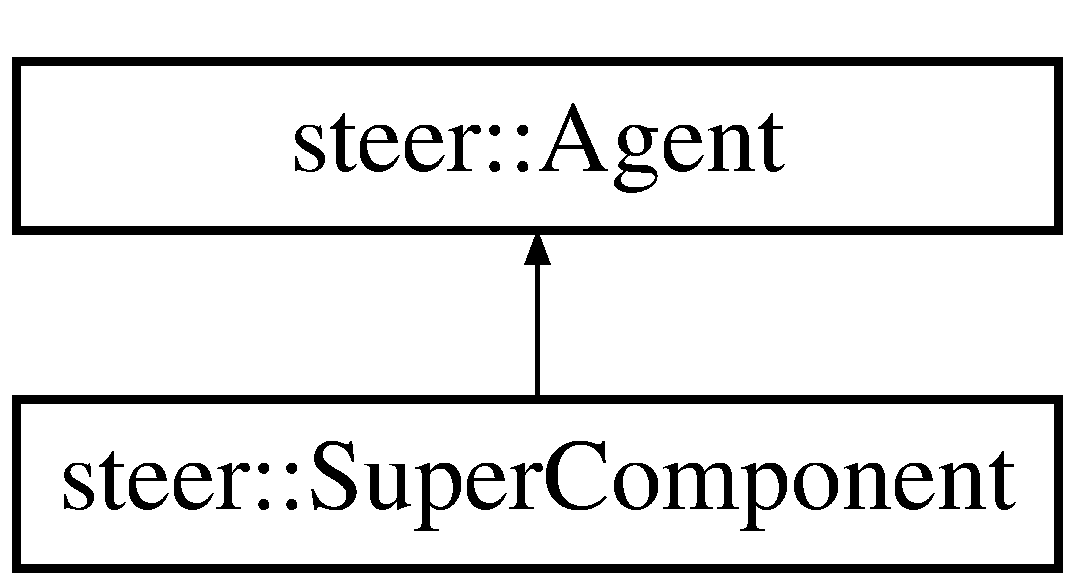
\includegraphics[height=2.000000cm]{classsteer_1_1_super_component}
\end{center}
\end{figure}
\subsection*{Public Member Functions}
\begin{DoxyCompactItemize}
\item 
\hypertarget{classsteer_1_1_super_component_a68178cb95e90ba293dbadc23a4f3059c}{{\bfseries Super\-Component} (\hyperlink{structsteer_1_1_behavior_parameters}{steer\-::\-Behavior\-Parameters} $\ast$params)}\label{classsteer_1_1_super_component_a68178cb95e90ba293dbadc23a4f3059c}

\item 
\hypertarget{classsteer_1_1_super_component_a694aa0c8a460e55f6528469c5b0472fe}{void {\bfseries set\-Params} (\hyperlink{structsteer_1_1_behavior_parameters}{steer\-::\-Behavior\-Parameters} $\ast$params)}\label{classsteer_1_1_super_component_a694aa0c8a460e55f6528469c5b0472fe}

\item 
\hypertarget{classsteer_1_1_super_component_aa2c67084990f7bf55d2145d11a10c7b1}{\hyperlink{structsteer_1_1_behavior_parameters}{steer\-::\-Behavior\-Parameters} $\ast$ {\bfseries get\-Params} ()}\label{classsteer_1_1_super_component_aa2c67084990f7bf55d2145d11a10c7b1}

\item 
\hypertarget{classsteer_1_1_super_component_a33741a52ba737cf3e9cfd57b4a57aebd}{void {\bfseries Update} (float dt)}\label{classsteer_1_1_super_component_a33741a52ba737cf3e9cfd57b4a57aebd}

\item 
\hypertarget{classsteer_1_1_super_component_a41007b4652393a035e711e24020e7f4d}{float \hyperlink{classsteer_1_1_super_component_a41007b4652393a035e711e24020e7f4d}{get\-Rotation} ()}\label{classsteer_1_1_super_component_a41007b4652393a035e711e24020e7f4d}

\begin{DoxyCompactList}\small\item\em Get the value of the seek component rotation. \end{DoxyCompactList}\item 
\hypertarget{classsteer_1_1_super_component_a21670f6217c1146ecbe2e7f634191987}{void {\bfseries set\-Neighbors} (std\-::vector$<$ \hyperlink{classsteer_1_1_super_component}{Super\-Component} $\ast$ $>$ $\ast$n)}\label{classsteer_1_1_super_component_a21670f6217c1146ecbe2e7f634191987}

\item 
\hypertarget{classsteer_1_1_super_component_a979f008e0d633b227b86341866f86a82}{std\-::vector$<$ \hyperlink{classsteer_1_1_super_component}{Super\-Component} $\ast$ $>$ $\ast$ {\bfseries get\-Neighbors} ()}\label{classsteer_1_1_super_component_a979f008e0d633b227b86341866f86a82}

\item 
\hypertarget{classsteer_1_1_super_component_ab5455f34959000eef1388e95784a9fa7}{void {\bfseries set\-Obstacles} (std\-::vector$<$ \hyperlink{classsteer_1_1_sphere_obstacle}{Sphere\-Obstacle} $\ast$ $>$ $\ast$o)}\label{classsteer_1_1_super_component_ab5455f34959000eef1388e95784a9fa7}

\item 
\hypertarget{classsteer_1_1_super_component_acd456febc86a0219468d1089479dc28e}{std\-::vector$<$ \hyperlink{classsteer_1_1_sphere_obstacle}{Sphere\-Obstacle} $\ast$ $>$ $\ast$ {\bfseries get\-Obstacles} ()}\label{classsteer_1_1_super_component_acd456febc86a0219468d1089479dc28e}

\item 
\hypertarget{classsteer_1_1_super_component_a8b708b58692f7aa2470869b8eb6662dc}{void {\bfseries set\-Walls} (std\-::vector$<$ \hyperlink{classsteer_1_1_wall}{Wall} $\ast$ $>$ $\ast$w)}\label{classsteer_1_1_super_component_a8b708b58692f7aa2470869b8eb6662dc}

\item 
\hypertarget{classsteer_1_1_super_component_a7b50fa401c00db5e8789dcece3e5f2df}{std\-::vector$<$ \hyperlink{classsteer_1_1_wall}{Wall} $\ast$ $>$ $\ast$ {\bfseries get\-Walls} ()}\label{classsteer_1_1_super_component_a7b50fa401c00db5e8789dcece3e5f2df}

\item 
\hypertarget{classsteer_1_1_super_component_a578bdae087432fc8da1a2d41e9050c43}{void {\bfseries set\-Path} (\hyperlink{classsteer_1_1_path}{steer\-::\-Path} $\ast$p)}\label{classsteer_1_1_super_component_a578bdae087432fc8da1a2d41e9050c43}

\item 
\hypertarget{classsteer_1_1_super_component_a9d3710528fcbcc4a20cfd3f03172e07e}{\hyperlink{classsteer_1_1_path}{steer\-::\-Path} $\ast$ {\bfseries get\-Path} () const }\label{classsteer_1_1_super_component_a9d3710528fcbcc4a20cfd3f03172e07e}

\item 
virtual bool \hyperlink{classsteer_1_1_super_component_a6d4b33b6f838d89216e11d8f2a427f58}{on} (\hyperlink{namespacesteer_afe6e72f8f8088962727051501181acbe}{steer\-::behavior\-Type} behavior) override
\begin{DoxyCompactList}\small\item\em This pure virtual function tests if a specific bit of m\-\_\-i\-Flags is set using bitwise operations. Must be overridden in derived classes. \end{DoxyCompactList}\item 
\hypertarget{classsteer_1_1_super_component_a95a9461aaa2c9d2ec66e2d39e982860f}{void {\bfseries alignment\-On} ()}\label{classsteer_1_1_super_component_a95a9461aaa2c9d2ec66e2d39e982860f}

\item 
\hypertarget{classsteer_1_1_super_component_a21047d726697e82d5ab3ec30a985549f}{void {\bfseries separation\-On} ()}\label{classsteer_1_1_super_component_a21047d726697e82d5ab3ec30a985549f}

\item 
\hypertarget{classsteer_1_1_super_component_a034287ad0a55f8b2487de596de12d4ce}{void {\bfseries cohesion\-On} ()}\label{classsteer_1_1_super_component_a034287ad0a55f8b2487de596de12d4ce}

\item 
\hypertarget{classsteer_1_1_super_component_a9533038d2966b62c5bdcf97df25be42d}{void {\bfseries seek\-On} ()}\label{classsteer_1_1_super_component_a9533038d2966b62c5bdcf97df25be42d}

\item 
\hypertarget{classsteer_1_1_super_component_aad1e8e1fe693457ca79e2b7dde1127ee}{void {\bfseries wander\-On} ()}\label{classsteer_1_1_super_component_aad1e8e1fe693457ca79e2b7dde1127ee}

\item 
\hypertarget{classsteer_1_1_super_component_a77f7d90c5f771385e6736078b98123b6}{void {\bfseries wall\-Avoidance\-On} ()}\label{classsteer_1_1_super_component_a77f7d90c5f771385e6736078b98123b6}

\item 
\hypertarget{classsteer_1_1_super_component_a5c9e56e9ba1ae2149961805602ae81d5}{void {\bfseries obstacle\-Avoidance\-On} ()}\label{classsteer_1_1_super_component_a5c9e56e9ba1ae2149961805602ae81d5}

\item 
\hypertarget{classsteer_1_1_super_component_a7acbabf640a1085bd85b9e5bad76afbd}{void {\bfseries pursuit\-On} ()}\label{classsteer_1_1_super_component_a7acbabf640a1085bd85b9e5bad76afbd}

\item 
\hypertarget{classsteer_1_1_super_component_a4dee8de9baec1cae50796a094c53ff98}{void {\bfseries offset\-Pursuit\-On} ()}\label{classsteer_1_1_super_component_a4dee8de9baec1cae50796a094c53ff98}

\item 
\hypertarget{classsteer_1_1_super_component_a8069592955f7feb75bdaf739775a53c9}{void {\bfseries interpose\-On} ()}\label{classsteer_1_1_super_component_a8069592955f7feb75bdaf739775a53c9}

\item 
\hypertarget{classsteer_1_1_super_component_a55aec2df40a718860690301807399ebc}{void {\bfseries hide\-On} ()}\label{classsteer_1_1_super_component_a55aec2df40a718860690301807399ebc}

\item 
\hypertarget{classsteer_1_1_super_component_afba2bd6ea6718e473a23f6b09e1d55a1}{void {\bfseries path\-Following\-On} ()}\label{classsteer_1_1_super_component_afba2bd6ea6718e473a23f6b09e1d55a1}

\item 
\hypertarget{classsteer_1_1_super_component_a692529db7b98c4dd941832e1c4447605}{void {\bfseries flee\-On} ()}\label{classsteer_1_1_super_component_a692529db7b98c4dd941832e1c4447605}

\item 
\hypertarget{classsteer_1_1_super_component_ae1356421fe88898957c2da286b1f5b57}{void {\bfseries evade\-On} ()}\label{classsteer_1_1_super_component_ae1356421fe88898957c2da286b1f5b57}

\item 
\hypertarget{classsteer_1_1_super_component_ad56441a92cff5e56290c42cd3468a62a}{void {\bfseries arrive\-On} ()}\label{classsteer_1_1_super_component_ad56441a92cff5e56290c42cd3468a62a}

\item 
\hypertarget{classsteer_1_1_super_component_aa4ebb59a05f6d76db805b1ad32959632}{void {\bfseries cohesion\-Off} ()}\label{classsteer_1_1_super_component_aa4ebb59a05f6d76db805b1ad32959632}

\item 
\hypertarget{classsteer_1_1_super_component_a433925dc720bf74738bd3ead6cefccd9}{void {\bfseries separation\-Off} ()}\label{classsteer_1_1_super_component_a433925dc720bf74738bd3ead6cefccd9}

\item 
\hypertarget{classsteer_1_1_super_component_a4a865469f2d39bbcef709c7532a0169a}{void {\bfseries alignment\-Off} ()}\label{classsteer_1_1_super_component_a4a865469f2d39bbcef709c7532a0169a}

\item 
\hypertarget{classsteer_1_1_super_component_a0540d3adfae4dc6c5a4fb1a9b821adae}{void {\bfseries seek\-Off} ()}\label{classsteer_1_1_super_component_a0540d3adfae4dc6c5a4fb1a9b821adae}

\item 
\hypertarget{classsteer_1_1_super_component_a73982065c3eb3e6d4e0335360f37fbb8}{void {\bfseries wander\-Off} ()}\label{classsteer_1_1_super_component_a73982065c3eb3e6d4e0335360f37fbb8}

\item 
\hypertarget{classsteer_1_1_super_component_a8a0ff1ca0ce03cae2c2885051d53bc75}{void {\bfseries wall\-Avoidance\-Off} ()}\label{classsteer_1_1_super_component_a8a0ff1ca0ce03cae2c2885051d53bc75}

\item 
\hypertarget{classsteer_1_1_super_component_a2574a6257fd6dbd4460cf6ed77cb8d28}{void {\bfseries obstacle\-Avoidance\-Off} ()}\label{classsteer_1_1_super_component_a2574a6257fd6dbd4460cf6ed77cb8d28}

\item 
\hypertarget{classsteer_1_1_super_component_a802631fd878ce6c2967570605c7f987d}{void {\bfseries pursuit\-Off} ()}\label{classsteer_1_1_super_component_a802631fd878ce6c2967570605c7f987d}

\item 
\hypertarget{classsteer_1_1_super_component_ac4e0a4756ad7775d3d01de7e406e8272}{void {\bfseries offset\-Pursuit\-Off} ()}\label{classsteer_1_1_super_component_ac4e0a4756ad7775d3d01de7e406e8272}

\item 
\hypertarget{classsteer_1_1_super_component_a3f45f753eddeb97abfbc29b4a1f77b75}{void {\bfseries interpose\-Off} ()}\label{classsteer_1_1_super_component_a3f45f753eddeb97abfbc29b4a1f77b75}

\item 
\hypertarget{classsteer_1_1_super_component_ab1de0a298d5dfecca12d1f17afaf574b}{void {\bfseries hide\-Off} ()}\label{classsteer_1_1_super_component_ab1de0a298d5dfecca12d1f17afaf574b}

\item 
\hypertarget{classsteer_1_1_super_component_aa7448c45c3f81bd5b0a24d9e6e50ffbc}{void {\bfseries path\-Following\-Off} ()}\label{classsteer_1_1_super_component_aa7448c45c3f81bd5b0a24d9e6e50ffbc}

\item 
\hypertarget{classsteer_1_1_super_component_af4f642a12cfdfd66bae01e964c65f969}{void {\bfseries flee\-Off} ()}\label{classsteer_1_1_super_component_af4f642a12cfdfd66bae01e964c65f969}

\item 
\hypertarget{classsteer_1_1_super_component_ad426e19bff42b63aefd3f475d9defef9}{void {\bfseries evade\-Off} ()}\label{classsteer_1_1_super_component_ad426e19bff42b63aefd3f475d9defef9}

\item 
\hypertarget{classsteer_1_1_super_component_a618abbb400ecc0aa2d16324aace4346d}{void {\bfseries arrive\-Off} ()}\label{classsteer_1_1_super_component_a618abbb400ecc0aa2d16324aace4346d}

\item 
\hypertarget{classsteer_1_1_super_component_af37bdcdae8312d2861fcadefff86750c}{bool {\bfseries is\-Cohesion\-On} ()}\label{classsteer_1_1_super_component_af37bdcdae8312d2861fcadefff86750c}

\item 
\hypertarget{classsteer_1_1_super_component_a7fd525d297e525111f00bba036b8265a}{bool {\bfseries is\-Separation\-On} ()}\label{classsteer_1_1_super_component_a7fd525d297e525111f00bba036b8265a}

\item 
\hypertarget{classsteer_1_1_super_component_a6ab1d4070e643d853869dc657138d2bd}{bool {\bfseries is\-Alignment\-On} ()}\label{classsteer_1_1_super_component_a6ab1d4070e643d853869dc657138d2bd}

\item 
\hypertarget{classsteer_1_1_super_component_add7c3aecb593103f9f55d337d3add830}{bool {\bfseries is\-Seek\-On} ()}\label{classsteer_1_1_super_component_add7c3aecb593103f9f55d337d3add830}

\item 
\hypertarget{classsteer_1_1_super_component_adf0459eb6fbf34b8b949abdc8eba2eb4}{bool {\bfseries is\-Wander\-On} ()}\label{classsteer_1_1_super_component_adf0459eb6fbf34b8b949abdc8eba2eb4}

\item 
\hypertarget{classsteer_1_1_super_component_a6f0f9abb497f25ba64130dca199facad}{bool {\bfseries is\-Wall\-Avoidance\-On} ()}\label{classsteer_1_1_super_component_a6f0f9abb497f25ba64130dca199facad}

\item 
\hypertarget{classsteer_1_1_super_component_a97ad5a6170d4f68a526eda3f2dfdf420}{bool {\bfseries is\-Obstacle\-Avoidance\-On} ()}\label{classsteer_1_1_super_component_a97ad5a6170d4f68a526eda3f2dfdf420}

\item 
\hypertarget{classsteer_1_1_super_component_a3d09457f210e696ce693c9c04f5c36d6}{bool {\bfseries is\-Flocking\-On} ()}\label{classsteer_1_1_super_component_a3d09457f210e696ce693c9c04f5c36d6}

\item 
\hypertarget{classsteer_1_1_super_component_a293c72beedcbc14b85705f8c9ecd233b}{bool {\bfseries is\-Pursuit\-On} ()}\label{classsteer_1_1_super_component_a293c72beedcbc14b85705f8c9ecd233b}

\item 
\hypertarget{classsteer_1_1_super_component_a1cba3443583722a5cdf2501cb0ff679c}{bool {\bfseries is\-Offset\-Pursuit\-On} ()}\label{classsteer_1_1_super_component_a1cba3443583722a5cdf2501cb0ff679c}

\item 
\hypertarget{classsteer_1_1_super_component_aea3b652a3ab5288e4a7c6a7dd47dc4bb}{bool {\bfseries is\-Interpose\-On} ()}\label{classsteer_1_1_super_component_aea3b652a3ab5288e4a7c6a7dd47dc4bb}

\item 
\hypertarget{classsteer_1_1_super_component_acabab07d95095686aa7a7bf4b6325e35}{bool {\bfseries is\-Hide\-On} ()}\label{classsteer_1_1_super_component_acabab07d95095686aa7a7bf4b6325e35}

\item 
\hypertarget{classsteer_1_1_super_component_a694ef730d59e91fb019835cd6c7d32cf}{bool {\bfseries is\-Path\-Following\-On} ()}\label{classsteer_1_1_super_component_a694ef730d59e91fb019835cd6c7d32cf}

\item 
\hypertarget{classsteer_1_1_super_component_a68819a55f2b757ca855c2317e125b829}{bool {\bfseries is\-Flee\-On} ()}\label{classsteer_1_1_super_component_a68819a55f2b757ca855c2317e125b829}

\item 
\hypertarget{classsteer_1_1_super_component_a7598a658f5ce09f8272f2ded8ca394cf}{bool {\bfseries is\-Evade\-On} ()}\label{classsteer_1_1_super_component_a7598a658f5ce09f8272f2ded8ca394cf}

\item 
\hypertarget{classsteer_1_1_super_component_a7ef0e1e6e643e06ed558b68e306c6ffa}{bool {\bfseries is\-Arrive\-On} ()}\label{classsteer_1_1_super_component_a7ef0e1e6e643e06ed558b68e306c6ffa}

\item 
\hypertarget{classsteer_1_1_super_component_aa3368b5600e8de4450e9c6b6db557f81}{void {\bfseries flocking\-On} ()}\label{classsteer_1_1_super_component_aa3368b5600e8de4450e9c6b6db557f81}

\item 
\hypertarget{classsteer_1_1_super_component_ab92db6c53f2a4454ab762be90af53d07}{void {\bfseries flocking\-Off} ()}\label{classsteer_1_1_super_component_ab92db6c53f2a4454ab762be90af53d07}

\item 
\hypertarget{classsteer_1_1_super_component_acd094527592bddd27b80b30026f0f474}{bool {\bfseries target\-Acquired} ()}\label{classsteer_1_1_super_component_acd094527592bddd27b80b30026f0f474}

\item 
\hypertarget{classsteer_1_1_super_component_a0664f84f96494841f4f0da7a11d299ea}{void {\bfseries set\-Evade\-Agent} (\hyperlink{classsteer_1_1_agent}{steer\-::\-Agent} $\ast$a)}\label{classsteer_1_1_super_component_a0664f84f96494841f4f0da7a11d299ea}

\item 
\hypertarget{classsteer_1_1_super_component_a4526494dd5beb03038495e0d23ef9f5a}{\hyperlink{classsteer_1_1_agent}{steer\-::\-Agent} $\ast$ {\bfseries get\-Evade\-Agent} () const }\label{classsteer_1_1_super_component_a4526494dd5beb03038495e0d23ef9f5a}

\item 
\hypertarget{classsteer_1_1_super_component_a7aeb081585a3126c91468184b1485d39}{void {\bfseries set\-Pursuit\-Agent} (\hyperlink{classsteer_1_1_agent}{steer\-::\-Agent} $\ast$a)}\label{classsteer_1_1_super_component_a7aeb081585a3126c91468184b1485d39}

\item 
\hypertarget{classsteer_1_1_super_component_abde4df825e54ee1b7dd612947182c73c}{\hyperlink{classsteer_1_1_agent}{steer\-::\-Agent} $\ast$ {\bfseries get\-Pursuit\-Agent} () const }\label{classsteer_1_1_super_component_abde4df825e54ee1b7dd612947182c73c}

\item 
\hypertarget{classsteer_1_1_super_component_ac6e8260adba8788734c07fabcd1d846a}{void {\bfseries set\-Leader} (\hyperlink{classsteer_1_1_agent}{steer\-::\-Agent} $\ast$l)}\label{classsteer_1_1_super_component_ac6e8260adba8788734c07fabcd1d846a}

\item 
\hypertarget{classsteer_1_1_super_component_a50f71ec70224b10c71241ef7bbdcabe4}{\hyperlink{classsteer_1_1_agent}{steer\-::\-Agent} $\ast$ {\bfseries get\-Leader} () const }\label{classsteer_1_1_super_component_a50f71ec70224b10c71241ef7bbdcabe4}

\item 
\hypertarget{classsteer_1_1_super_component_af024f5ae5b4d77e93a576806be160903}{void {\bfseries set\-Interpose\-Agents} (\hyperlink{classsteer_1_1_agent}{steer\-::\-Agent} $\ast$a, \hyperlink{classsteer_1_1_agent}{steer\-::\-Agent} $\ast$b)}\label{classsteer_1_1_super_component_af024f5ae5b4d77e93a576806be160903}

\item 
\hypertarget{classsteer_1_1_super_component_ad9e2774c665eec1727f2cd0ddd763705}{void {\bfseries set\-Interpose\-Agent\-A} (\hyperlink{classsteer_1_1_agent}{steer\-::\-Agent} $\ast$a)}\label{classsteer_1_1_super_component_ad9e2774c665eec1727f2cd0ddd763705}

\item 
\hypertarget{classsteer_1_1_super_component_a98d56c5408bf60bdb6f4a60194e94564}{void {\bfseries set\-Interpose\-Agent\-B} (\hyperlink{classsteer_1_1_agent}{steer\-::\-Agent} $\ast$b)}\label{classsteer_1_1_super_component_a98d56c5408bf60bdb6f4a60194e94564}

\item 
\hypertarget{classsteer_1_1_super_component_a43f0c97eab839cf58023b9228a37f65c}{\hyperlink{classsteer_1_1_agent}{steer\-::\-Agent} $\ast$ {\bfseries get\-Interpose\-Agent\-A} () const }\label{classsteer_1_1_super_component_a43f0c97eab839cf58023b9228a37f65c}

\item 
\hypertarget{classsteer_1_1_super_component_a6b5c49bf65787f4018617a190da00c09}{\hyperlink{classsteer_1_1_agent}{steer\-::\-Agent} $\ast$ {\bfseries get\-Interpose\-Agent\-B} () const }\label{classsteer_1_1_super_component_a6b5c49bf65787f4018617a190da00c09}

\item 
\hypertarget{classsteer_1_1_super_component_ae26c82ac84ec2ec52efe741bb842b736}{void {\bfseries set\-Hide\-Agent} (\hyperlink{classsteer_1_1_agent}{steer\-::\-Agent} $\ast$a)}\label{classsteer_1_1_super_component_ae26c82ac84ec2ec52efe741bb842b736}

\item 
\hypertarget{classsteer_1_1_super_component_ad3e3d4efee10538f61b36df6d7512381}{\hyperlink{classsteer_1_1_agent}{steer\-::\-Agent} $\ast$ {\bfseries get\-Hide\-Agent} () const }\label{classsteer_1_1_super_component_ad3e3d4efee10538f61b36df6d7512381}

\item 
\hypertarget{classsteer_1_1_super_component_a934b715dfccce23a5cec1f6e462f985c}{virtual \hyperlink{structsteer_1_1_vector2}{Vector2} \hyperlink{classsteer_1_1_super_component_a934b715dfccce23a5cec1f6e462f985c}{Calculate} () override}\label{classsteer_1_1_super_component_a934b715dfccce23a5cec1f6e462f985c}

\begin{DoxyCompactList}\small\item\em A pure virtual method for calculating the steering vector. \end{DoxyCompactList}\item 
\hypertarget{classsteer_1_1_super_component_ace499f2a223579802a562c4fa91d677b}{virtual \hyperlink{structsteer_1_1_vector2}{Vector2} {\bfseries calculate\-Weighted\-Sum} () override}\label{classsteer_1_1_super_component_ace499f2a223579802a562c4fa91d677b}

\end{DoxyCompactItemize}
\subsection*{Public Attributes}
\begin{DoxyCompactItemize}
\item 
\hypertarget{classsteer_1_1_super_component_aaced68de7b8442857e548a9a3c6db1e3}{float \hyperlink{classsteer_1_1_super_component_aaced68de7b8442857e548a9a3c6db1e3}{m\-\_\-weight\-Seek}}\label{classsteer_1_1_super_component_aaced68de7b8442857e548a9a3c6db1e3}

\begin{DoxyCompactList}\small\item\em Multiplier -\/ can be adjusted to effect strength of the seeking behavior. \end{DoxyCompactList}\item 
\hypertarget{classsteer_1_1_super_component_ac9472b29bf3a879877bb89904671a90a}{float \hyperlink{classsteer_1_1_super_component_ac9472b29bf3a879877bb89904671a90a}{m\-\_\-weight\-Flee}}\label{classsteer_1_1_super_component_ac9472b29bf3a879877bb89904671a90a}

\begin{DoxyCompactList}\small\item\em Multiplier -\/ can be adjusted to effect strength of the fleeing behavior. \end{DoxyCompactList}\item 
\hypertarget{classsteer_1_1_super_component_a17fd146cff611cfd6d01dafca41e454e}{float \hyperlink{classsteer_1_1_super_component_a17fd146cff611cfd6d01dafca41e454e}{m\-\_\-weight\-Arrive}}\label{classsteer_1_1_super_component_a17fd146cff611cfd6d01dafca41e454e}

\begin{DoxyCompactList}\small\item\em Multiplier -\/ can be adjusted to effect strength of the arriving behavior. \end{DoxyCompactList}\item 
\hypertarget{classsteer_1_1_super_component_a145b3e02c139711b4137c0270116a621}{float \hyperlink{classsteer_1_1_super_component_a145b3e02c139711b4137c0270116a621}{m\-\_\-weight\-Pursuit}}\label{classsteer_1_1_super_component_a145b3e02c139711b4137c0270116a621}

\begin{DoxyCompactList}\small\item\em Multiplier -\/ can be adjusted to effect strength of the pursuing behavior. \end{DoxyCompactList}\item 
\hypertarget{classsteer_1_1_super_component_ac5d3901b71460a9058237289148ec9b3}{float \hyperlink{classsteer_1_1_super_component_ac5d3901b71460a9058237289148ec9b3}{m\-\_\-weight\-Evade}}\label{classsteer_1_1_super_component_ac5d3901b71460a9058237289148ec9b3}

\begin{DoxyCompactList}\small\item\em Multiplier -\/ can be adjusted to effect strength of the evading behavior. \end{DoxyCompactList}\item 
\hypertarget{classsteer_1_1_super_component_a10d96235f4dc1b8f94e493cfb4467a87}{float \hyperlink{classsteer_1_1_super_component_a10d96235f4dc1b8f94e493cfb4467a87}{m\-\_\-weight\-Interpose}}\label{classsteer_1_1_super_component_a10d96235f4dc1b8f94e493cfb4467a87}

\begin{DoxyCompactList}\small\item\em Multiplier -\/ can be adjusted to effect strength of the interposing behavior. \end{DoxyCompactList}\item 
\hypertarget{classsteer_1_1_super_component_a478260491716990f52554d9afb914bfe}{float \hyperlink{classsteer_1_1_super_component_a478260491716990f52554d9afb914bfe}{m\-\_\-weight\-Hide}}\label{classsteer_1_1_super_component_a478260491716990f52554d9afb914bfe}

\begin{DoxyCompactList}\small\item\em Multiplier -\/ can be adjusted to effect strength of the hiding behavior. \end{DoxyCompactList}\item 
\hypertarget{classsteer_1_1_super_component_a5271df7b865469ee56b9aca54ac07fe1}{float \hyperlink{classsteer_1_1_super_component_a5271df7b865469ee56b9aca54ac07fe1}{m\-\_\-weight\-Offset\-Pursuit}}\label{classsteer_1_1_super_component_a5271df7b865469ee56b9aca54ac07fe1}

\begin{DoxyCompactList}\small\item\em Multiplier -\/ can be adjusted to effect strength of the offset pursuit behavior. \end{DoxyCompactList}\item 
\hypertarget{classsteer_1_1_super_component_a0d14d90f7ad370e3e64abeed5eaaa459}{float \hyperlink{classsteer_1_1_super_component_a0d14d90f7ad370e3e64abeed5eaaa459}{m\-\_\-weight\-Wander}}\label{classsteer_1_1_super_component_a0d14d90f7ad370e3e64abeed5eaaa459}

\begin{DoxyCompactList}\small\item\em Multiplier -\/ can be adjusted to effect strength of the wander behavior. \end{DoxyCompactList}\item 
\hypertarget{classsteer_1_1_super_component_aae596167a99efd22caee49eda457b4d1}{float \hyperlink{classsteer_1_1_super_component_aae596167a99efd22caee49eda457b4d1}{m\-\_\-weight\-Alignment}}\label{classsteer_1_1_super_component_aae596167a99efd22caee49eda457b4d1}

\begin{DoxyCompactList}\small\item\em Multiplier -\/ can be adjusted to effect strength of the alignment behavior. \end{DoxyCompactList}\item 
\hypertarget{classsteer_1_1_super_component_a6a40ec5da6af1b7f36ba023c28456972}{float \hyperlink{classsteer_1_1_super_component_a6a40ec5da6af1b7f36ba023c28456972}{m\-\_\-weight\-Separation}}\label{classsteer_1_1_super_component_a6a40ec5da6af1b7f36ba023c28456972}

\begin{DoxyCompactList}\small\item\em Multiplier -\/ can be adjusted to effect strength of the separation behavior. \end{DoxyCompactList}\item 
\hypertarget{classsteer_1_1_super_component_af026be44b85a808ebf9eca9e8bb2f070}{float \hyperlink{classsteer_1_1_super_component_af026be44b85a808ebf9eca9e8bb2f070}{m\-\_\-weight\-Cohesion}}\label{classsteer_1_1_super_component_af026be44b85a808ebf9eca9e8bb2f070}

\begin{DoxyCompactList}\small\item\em Multiplier -\/ can be adjusted to effect strength of the cohesion behavior. \end{DoxyCompactList}\item 
\hypertarget{classsteer_1_1_super_component_ab38d5c6fa86e882bef3258d4ee5542f4}{float \hyperlink{classsteer_1_1_super_component_ab38d5c6fa86e882bef3258d4ee5542f4}{m\-\_\-weight\-Obstacle\-Avoidance}}\label{classsteer_1_1_super_component_ab38d5c6fa86e882bef3258d4ee5542f4}

\begin{DoxyCompactList}\small\item\em Multiplier -\/ can be adjusted to effect strength of the obstacle avoidance behavior. \end{DoxyCompactList}\item 
\hypertarget{classsteer_1_1_super_component_a801a719fc8fcec34ec4a8ef0b6c11800}{float \hyperlink{classsteer_1_1_super_component_a801a719fc8fcec34ec4a8ef0b6c11800}{m\-\_\-weight\-Wall\-Avoidance}}\label{classsteer_1_1_super_component_a801a719fc8fcec34ec4a8ef0b6c11800}

\begin{DoxyCompactList}\small\item\em Multiplier -\/ can be adjusted to effect strength of the wall avoidance behavior. \end{DoxyCompactList}\item 
\hypertarget{classsteer_1_1_super_component_aab01c9677fa02f20cccb8a7c74a8c7a8}{float \hyperlink{classsteer_1_1_super_component_aab01c9677fa02f20cccb8a7c74a8c7a8}{m\-\_\-weight\-Path\-Following}}\label{classsteer_1_1_super_component_aab01c9677fa02f20cccb8a7c74a8c7a8}

\begin{DoxyCompactList}\small\item\em Multiplier -\/ can be adjusted to effect strength of the \hyperlink{classsteer_1_1_path}{Path} Following behavior. \end{DoxyCompactList}\end{DoxyCompactItemize}


\subsection{Detailed Description}
An example implementation of the an agent with every steering behavior implemented. 

\subsection{Member Function Documentation}
\hypertarget{classsteer_1_1_super_component_a6d4b33b6f838d89216e11d8f2a427f58}{\index{steer\-::\-Super\-Component@{steer\-::\-Super\-Component}!on@{on}}
\index{on@{on}!steer::SuperComponent@{steer\-::\-Super\-Component}}
\subsubsection[{on}]{\setlength{\rightskip}{0pt plus 5cm}virtual bool steer\-::\-Super\-Component\-::on (
\begin{DoxyParamCaption}
\item[{{\bf steer\-::behavior\-Type}}]{behavior}
\end{DoxyParamCaption}
)\hspace{0.3cm}{\ttfamily [inline]}, {\ttfamily [override]}, {\ttfamily [virtual]}}}\label{classsteer_1_1_super_component_a6d4b33b6f838d89216e11d8f2a427f58}


This pure virtual function tests if a specific bit of m\-\_\-i\-Flags is set using bitwise operations. Must be overridden in derived classes. 


\begin{DoxyParams}{Parameters}
{\em behavior} & -\/ enum behavior\-Type. \\
\hline
\end{DoxyParams}


Implements \hyperlink{classsteer_1_1_agent_a707204e49e6519c7a8ea0f3ded608d98}{steer\-::\-Agent}.



The documentation for this class was generated from the following files\-:\begin{DoxyCompactItemize}
\item 
include/steeriously/components/Super\-Component.\-hpp\item 
src/steeriously/components/Super\-Component.\-cpp\end{DoxyCompactItemize}

\hypertarget{structsteer_1_1_vector2}{\section{steer\-:\-:Vector2 Struct Reference}
\label{structsteer_1_1_vector2}\index{steer\-::\-Vector2@{steer\-::\-Vector2}}
}


A 2\-D vector struct used in many steering calculations.  




{\ttfamily \#include $<$Vector2.\-hpp$>$}

\subsection*{Public Member Functions}
\begin{DoxyCompactItemize}
\item 
\hypertarget{structsteer_1_1_vector2_a6a933cf0f06bfd06c87504afadb2fb1f}{\hyperlink{structsteer_1_1_vector2_a6a933cf0f06bfd06c87504afadb2fb1f}{Vector2} ()}\label{structsteer_1_1_vector2_a6a933cf0f06bfd06c87504afadb2fb1f}

\begin{DoxyCompactList}\small\item\em Default constructor. \end{DoxyCompactList}\item 
\hypertarget{structsteer_1_1_vector2_a9a52d06e412d058cd153d39ce2f4f8e6}{{\bfseries Vector2} (double a, double b)}\label{structsteer_1_1_vector2_a9a52d06e412d058cd153d39ce2f4f8e6}

\item 
\hypertarget{structsteer_1_1_vector2_acfdeb77fde9e5ff5b4d4382cedae7c37}{void \hyperlink{structsteer_1_1_vector2_acfdeb77fde9e5ff5b4d4382cedae7c37}{Zero} ()}\label{structsteer_1_1_vector2_acfdeb77fde9e5ff5b4d4382cedae7c37}

\begin{DoxyCompactList}\small\item\em Set both x and y values to zero. \end{DoxyCompactList}\item 
\hypertarget{structsteer_1_1_vector2_ac566f4b8db067347553e267e52124360}{bool \hyperlink{structsteer_1_1_vector2_ac566f4b8db067347553e267e52124360}{is\-Zero} () const }\label{structsteer_1_1_vector2_ac566f4b8db067347553e267e52124360}

\begin{DoxyCompactList}\small\item\em Returns true if both x and y values are zero. \end{DoxyCompactList}\item 
\hypertarget{structsteer_1_1_vector2_abd9e9306146a4ac7b26bb3b10a438d73}{double \hyperlink{structsteer_1_1_vector2_abd9e9306146a4ac7b26bb3b10a438d73}{Length} () const }\label{structsteer_1_1_vector2_abd9e9306146a4ac7b26bb3b10a438d73}

\begin{DoxyCompactList}\small\item\em Returns the length of the vector. \end{DoxyCompactList}\item 
\hypertarget{structsteer_1_1_vector2_af8eb7d1603dcf6e474ee65877649db47}{double \hyperlink{structsteer_1_1_vector2_af8eb7d1603dcf6e474ee65877649db47}{Length\-Sq} () const }\label{structsteer_1_1_vector2_af8eb7d1603dcf6e474ee65877649db47}

\begin{DoxyCompactList}\small\item\em Returns the squared length of the vector (thereby avoiding sqrt). \end{DoxyCompactList}\item 
\hypertarget{structsteer_1_1_vector2_a7a18e52012cf852487e3923c5e902739}{void \hyperlink{structsteer_1_1_vector2_a7a18e52012cf852487e3923c5e902739}{Normalize} ()}\label{structsteer_1_1_vector2_a7a18e52012cf852487e3923c5e902739}

\begin{DoxyCompactList}\small\item\em Normalizes the vector. \end{DoxyCompactList}\item 
\hypertarget{structsteer_1_1_vector2_ac2fa511713c43bd4d8a5d7d431acfbb4}{double \hyperlink{structsteer_1_1_vector2_ac2fa511713c43bd4d8a5d7d431acfbb4}{Dot} (const \hyperlink{structsteer_1_1_vector2}{Vector2} \&v2) const }\label{structsteer_1_1_vector2_ac2fa511713c43bd4d8a5d7d431acfbb4}

\begin{DoxyCompactList}\small\item\em Returns the dot product of the vector. \end{DoxyCompactList}\item 
\hypertarget{structsteer_1_1_vector2_a930a20a650638870219deee45b01f94f}{int \hyperlink{structsteer_1_1_vector2_a930a20a650638870219deee45b01f94f}{Sign} (const \hyperlink{structsteer_1_1_vector2}{Vector2} \&v2) const }\label{structsteer_1_1_vector2_a930a20a650638870219deee45b01f94f}

\begin{DoxyCompactList}\small\item\em Returns positive if v2 is clockwise of this vector, negative if anticlockwise (assuming y-\/axis is pointing down and x-\/axis is pointing right). \end{DoxyCompactList}\item 
\hypertarget{structsteer_1_1_vector2_ad2319dbb015ad83c94ed876a5deaf4f2}{\hyperlink{structsteer_1_1_vector2}{Vector2} \hyperlink{structsteer_1_1_vector2_ad2319dbb015ad83c94ed876a5deaf4f2}{Perp} () const }\label{structsteer_1_1_vector2_ad2319dbb015ad83c94ed876a5deaf4f2}

\begin{DoxyCompactList}\small\item\em Returns the vector that is perpendicular to this vector. \end{DoxyCompactList}\item 
\hypertarget{structsteer_1_1_vector2_a92845bc9c24cb14bbb1ae3702b626ef3}{void {\bfseries Truncate} (double max)}\label{structsteer_1_1_vector2_a92845bc9c24cb14bbb1ae3702b626ef3}

\item 
\hypertarget{structsteer_1_1_vector2_a970134ff890ad7bf153843000a76215c}{double {\bfseries Distance} (const \hyperlink{structsteer_1_1_vector2}{Vector2} \&v2) const }\label{structsteer_1_1_vector2_a970134ff890ad7bf153843000a76215c}

\item 
\hypertarget{structsteer_1_1_vector2_a1a6c9ab976c106ec78119178136659dd}{double {\bfseries Distance\-Sq} (const \hyperlink{structsteer_1_1_vector2}{Vector2} \&v2) const }\label{structsteer_1_1_vector2_a1a6c9ab976c106ec78119178136659dd}

\item 
\hypertarget{structsteer_1_1_vector2_aa2379c044c2f75d22d359261316dd58d}{void {\bfseries Reflect} (const \hyperlink{structsteer_1_1_vector2}{Vector2} \&norm)}\label{structsteer_1_1_vector2_aa2379c044c2f75d22d359261316dd58d}

\item 
\hypertarget{structsteer_1_1_vector2_addebc491cb942193b6a5699747ab75fe}{\hyperlink{structsteer_1_1_vector2}{Vector2} {\bfseries Get\-Reverse} () const }\label{structsteer_1_1_vector2_addebc491cb942193b6a5699747ab75fe}

\item 
\hypertarget{structsteer_1_1_vector2_ae69f4a22a7d3afc6b51d940c23a9e53e}{const \hyperlink{structsteer_1_1_vector2}{Vector2} \& {\bfseries operator+=} (const \hyperlink{structsteer_1_1_vector2}{Vector2} \&rhs)}\label{structsteer_1_1_vector2_ae69f4a22a7d3afc6b51d940c23a9e53e}

\item 
\hypertarget{structsteer_1_1_vector2_a3463f6acec1d0128e4df31e2bfe7e85d}{const \hyperlink{structsteer_1_1_vector2}{Vector2} \& {\bfseries operator-\/=} (const \hyperlink{structsteer_1_1_vector2}{Vector2} \&rhs)}\label{structsteer_1_1_vector2_a3463f6acec1d0128e4df31e2bfe7e85d}

\item 
\hypertarget{structsteer_1_1_vector2_aae8fe5be70d98313785f7982aaa1e017}{const \hyperlink{structsteer_1_1_vector2}{Vector2} \& {\bfseries operator$\ast$=} (const double \&rhs)}\label{structsteer_1_1_vector2_aae8fe5be70d98313785f7982aaa1e017}

\item 
\hypertarget{structsteer_1_1_vector2_a7491e13d88f2f028445fa2218b62bb03}{const \hyperlink{structsteer_1_1_vector2}{Vector2} \& {\bfseries operator/=} (const double \&rhs)}\label{structsteer_1_1_vector2_a7491e13d88f2f028445fa2218b62bb03}

\item 
\hypertarget{structsteer_1_1_vector2_a797fa0001eaaafe3eb90a260f6320c60}{bool {\bfseries operator==} (const \hyperlink{structsteer_1_1_vector2}{Vector2} \&rhs) const }\label{structsteer_1_1_vector2_a797fa0001eaaafe3eb90a260f6320c60}

\item 
\hypertarget{structsteer_1_1_vector2_a667ff2b4dc594a07e19f766dc83125c0}{bool {\bfseries operator!=} (const \hyperlink{structsteer_1_1_vector2}{Vector2} \&rhs) const }\label{structsteer_1_1_vector2_a667ff2b4dc594a07e19f766dc83125c0}

\end{DoxyCompactItemize}
\subsection*{Public Attributes}
\begin{DoxyCompactItemize}
\item 
\hypertarget{structsteer_1_1_vector2_ab7cf735c31ffd694787bf4f611691e3e}{double {\bfseries x}}\label{structsteer_1_1_vector2_ab7cf735c31ffd694787bf4f611691e3e}

\item 
\hypertarget{structsteer_1_1_vector2_a47852c01f7b228b5c18515e27ba5a394}{double {\bfseries y}}\label{structsteer_1_1_vector2_a47852c01f7b228b5c18515e27ba5a394}

\end{DoxyCompactItemize}


\subsection{Detailed Description}
A 2\-D vector struct used in many steering calculations. 

The documentation for this struct was generated from the following file\-:\begin{DoxyCompactItemize}
\item 
include/steeriously/Vector2.\-hpp\end{DoxyCompactItemize}

\hypertarget{classsteer_1_1_vector_math}{\section{steer\-:\-:Vector\-Math Class Reference}
\label{classsteer_1_1_vector_math}\index{steer\-::\-Vector\-Math@{steer\-::\-Vector\-Math}}
}


Stateless \hyperlink{classsteer_1_1_vector_math}{Vector\-Math} class utilizing static methods to manipulate vectors. \par
Copies of \hyperlink{structsteer_1_1_vector2}{Vector2} are cheap, therefore all functions are \char`\"{}pass by value\char`\"{} at this time.  




{\ttfamily \#include $<$Vector\-Math.\-hpp$>$}

\subsection*{Public Member Functions}
\begin{DoxyCompactItemize}
\item 
\hypertarget{classsteer_1_1_vector_math_afa46a599077253d47819d92e0be8d383}{\hyperlink{classsteer_1_1_vector_math_afa46a599077253d47819d92e0be8d383}{Vector\-Math} ()}\label{classsteer_1_1_vector_math_afa46a599077253d47819d92e0be8d383}

\begin{DoxyCompactList}\small\item\em Constructor. \end{DoxyCompactList}\item 
\hypertarget{classsteer_1_1_vector_math_a311193142786d1f4904dd6de3146b474}{\hyperlink{classsteer_1_1_vector_math_a311193142786d1f4904dd6de3146b474}{$\sim$\-Vector\-Math} ()}\label{classsteer_1_1_vector_math_a311193142786d1f4904dd6de3146b474}

\begin{DoxyCompactList}\small\item\em Destructor. \end{DoxyCompactList}\end{DoxyCompactItemize}
\subsection*{Static Public Member Functions}
\begin{DoxyCompactItemize}
\item 
static \hyperlink{structsteer_1_1_vector2}{Vector2} \hyperlink{classsteer_1_1_vector_math_a6a637fee6dd4c1fb239d78012e3e5a62}{component\-Product} (\hyperlink{structsteer_1_1_vector2}{Vector2} a, \hyperlink{structsteer_1_1_vector2}{Vector2} b)
\begin{DoxyCompactList}\small\item\em A static method returning a vector that is the component product of two vectors. \end{DoxyCompactList}\item 
static \hyperlink{structsteer_1_1_vector2}{Vector2} \hyperlink{classsteer_1_1_vector_math_ae2a61b5919c0b3e29d98add18340c5e3}{truncate} (\hyperlink{structsteer_1_1_vector2}{Vector2} v, float max)
\begin{DoxyCompactList}\small\item\em A static method returning a truncated vector based on some maximum value. \end{DoxyCompactList}\item 
static float \hyperlink{classsteer_1_1_vector_math_ae9646371fd7dd38c33ee2f88ac114234}{dot\-Product} (\hyperlink{structsteer_1_1_vector2}{Vector2} a, \hyperlink{structsteer_1_1_vector2}{Vector2} b)
\begin{DoxyCompactList}\small\item\em A static method returning the dot product of two vectors. \end{DoxyCompactList}\item 
static \hyperlink{structsteer_1_1_vector2}{Vector2} \hyperlink{classsteer_1_1_vector_math_aa2820b8424b7d01bcbaf877d05108fd2}{perpendicular} (\hyperlink{structsteer_1_1_vector2}{Vector2} a)
\begin{DoxyCompactList}\small\item\em A static method returning a vector that is perpendicular to the vector supplied. \end{DoxyCompactList}\item 
static \hyperlink{structsteer_1_1_vector2}{Vector2} \hyperlink{classsteer_1_1_vector_math_af1e8a61f7eb8fb2ba8fb7fe2fa5d59e9}{direction} (\hyperlink{structsteer_1_1_vector2}{Vector2} a, \hyperlink{structsteer_1_1_vector2}{Vector2} b)
\begin{DoxyCompactList}\small\item\em A static method returning the directional vector that vector a needs to be transformed to in order to point towards vector b. \end{DoxyCompactList}\item 
static float \hyperlink{classsteer_1_1_vector_math_a386d5cc8c572422ac7a2f63925883a06}{distance} (\hyperlink{structsteer_1_1_vector2}{Vector2} a, \hyperlink{structsteer_1_1_vector2}{Vector2} b)
\begin{DoxyCompactList}\small\item\em A static method returning the distance between two given vectors, a and b. \end{DoxyCompactList}\item 
static float \hyperlink{classsteer_1_1_vector_math_ab7c1336121423d029113b0314b48dc15}{distance\-Squared} (\hyperlink{structsteer_1_1_vector2}{Vector2} a, \hyperlink{structsteer_1_1_vector2}{Vector2} b)
\begin{DoxyCompactList}\small\item\em A static method returning the distance squared between two given vectors, a and b -\/ avoids the overhead of sqrt when necessary. \end{DoxyCompactList}\item 
static float \hyperlink{classsteer_1_1_vector_math_acd9482d3b672a34ddf90e20e94373bd5}{find\-Angle} (\hyperlink{structsteer_1_1_vector2}{Vector2} v)
\begin{DoxyCompactList}\small\item\em A static method returning the angle resolved from a vector (pass in vector1 -\/ vector2 or a precomputed vector) -\/ useful for finding the angle of a target, for example.\par
Internally, this function converts from radians to degrees so you don't have to. \end{DoxyCompactList}\item 
static float \hyperlink{classsteer_1_1_vector_math_a71fff49a5e48b59400a331283aa89adc}{length} (\hyperlink{structsteer_1_1_vector2}{Vector2} v)
\begin{DoxyCompactList}\small\item\em A static method returning the length (or magnitude) of a vector. \end{DoxyCompactList}\item 
static float \hyperlink{classsteer_1_1_vector_math_a70ef679a6a5e8ffeeaf8e37aa6510f65}{length\-Squared} (\hyperlink{structsteer_1_1_vector2}{Vector2} v)
\begin{DoxyCompactList}\small\item\em A static method returning the squared length of a vector. \end{DoxyCompactList}\item 
static \hyperlink{structsteer_1_1_vector2}{Vector2} \hyperlink{classsteer_1_1_vector_math_aae0d6aa81adba0a66ad40a43f71db6a3}{normalize} (\hyperlink{structsteer_1_1_vector2}{Vector2} v)
\begin{DoxyCompactList}\small\item\em A static method returning a normalized (or unit) vector. \end{DoxyCompactList}\item 
static bool \hyperlink{classsteer_1_1_vector_math_a2ba23731de0598131b003f9409d3d433}{line\-Intersects\-Circle} (\hyperlink{structsteer_1_1_vector2}{Vector2} ahead, \hyperlink{structsteer_1_1_vector2}{Vector2} ahead2, \hyperlink{classsteer_1_1_sphere_obstacle}{Sphere\-Obstacle} obstacle, \hyperlink{structsteer_1_1_vector2}{Vector2} agent\-Position)
\begin{DoxyCompactList}\small\item\em A static method returning a boolean to test whether a vector intersects a circle. \end{DoxyCompactList}\end{DoxyCompactItemize}


\subsection{Detailed Description}
Stateless \hyperlink{classsteer_1_1_vector_math}{Vector\-Math} class utilizing static methods to manipulate vectors. \par
Copies of \hyperlink{structsteer_1_1_vector2}{Vector2} are cheap, therefore all functions are \char`\"{}pass by value\char`\"{} at this time. 

\subsection{Member Function Documentation}
\hypertarget{classsteer_1_1_vector_math_a6a637fee6dd4c1fb239d78012e3e5a62}{\index{steer\-::\-Vector\-Math@{steer\-::\-Vector\-Math}!component\-Product@{component\-Product}}
\index{component\-Product@{component\-Product}!steer::VectorMath@{steer\-::\-Vector\-Math}}
\subsubsection[{component\-Product}]{\setlength{\rightskip}{0pt plus 5cm}{\bf Vector2} steer\-::\-Vector\-Math\-::component\-Product (
\begin{DoxyParamCaption}
\item[{{\bf Vector2}}]{a, }
\item[{{\bf Vector2}}]{b}
\end{DoxyParamCaption}
)\hspace{0.3cm}{\ttfamily [static]}}}\label{classsteer_1_1_vector_math_a6a637fee6dd4c1fb239d78012e3e5a62}


A static method returning a vector that is the component product of two vectors. 

\begin{DoxySeeAlso}{See Also}
static \hyperlink{structsteer_1_1_vector2}{Vector2} \hyperlink{classsteer_1_1_vector_math_a6a637fee6dd4c1fb239d78012e3e5a62}{component\-Product(\-Vector2 a, Vector2 b)} 
\end{DoxySeeAlso}

\begin{DoxyParams}{Parameters}
{\em a} & -\/ a vector of doubles. \\
\hline
{\em b} & -\/ a vector of doubles. \\
\hline
\end{DoxyParams}
\hypertarget{classsteer_1_1_vector_math_af1e8a61f7eb8fb2ba8fb7fe2fa5d59e9}{\index{steer\-::\-Vector\-Math@{steer\-::\-Vector\-Math}!direction@{direction}}
\index{direction@{direction}!steer::VectorMath@{steer\-::\-Vector\-Math}}
\subsubsection[{direction}]{\setlength{\rightskip}{0pt plus 5cm}{\bf Vector2} steer\-::\-Vector\-Math\-::direction (
\begin{DoxyParamCaption}
\item[{{\bf Vector2}}]{a, }
\item[{{\bf Vector2}}]{b}
\end{DoxyParamCaption}
)\hspace{0.3cm}{\ttfamily [static]}}}\label{classsteer_1_1_vector_math_af1e8a61f7eb8fb2ba8fb7fe2fa5d59e9}


A static method returning the directional vector that vector a needs to be transformed to in order to point towards vector b. 

\begin{DoxySeeAlso}{See Also}
static \hyperlink{structsteer_1_1_vector2}{Vector2} \hyperlink{classsteer_1_1_vector_math_af1e8a61f7eb8fb2ba8fb7fe2fa5d59e9}{direction(\-Vector2 a, Vector2 b)} 
\end{DoxySeeAlso}

\begin{DoxyParams}{Parameters}
{\em a} & -\/ a vector of doubles. \\
\hline
{\em b} & -\/ a vector of doubles. \\
\hline
\end{DoxyParams}
\hypertarget{classsteer_1_1_vector_math_a386d5cc8c572422ac7a2f63925883a06}{\index{steer\-::\-Vector\-Math@{steer\-::\-Vector\-Math}!distance@{distance}}
\index{distance@{distance}!steer::VectorMath@{steer\-::\-Vector\-Math}}
\subsubsection[{distance}]{\setlength{\rightskip}{0pt plus 5cm}float steer\-::\-Vector\-Math\-::distance (
\begin{DoxyParamCaption}
\item[{{\bf Vector2}}]{a, }
\item[{{\bf Vector2}}]{b}
\end{DoxyParamCaption}
)\hspace{0.3cm}{\ttfamily [static]}}}\label{classsteer_1_1_vector_math_a386d5cc8c572422ac7a2f63925883a06}


A static method returning the distance between two given vectors, a and b. 

\begin{DoxySeeAlso}{See Also}
static float \hyperlink{classsteer_1_1_vector_math_a386d5cc8c572422ac7a2f63925883a06}{distance(\-Vector2 a, Vector2 b)} 
\end{DoxySeeAlso}

\begin{DoxyParams}{Parameters}
{\em a} & -\/ a vector of doubles. \\
\hline
{\em b} & -\/ a vector of doubles. \\
\hline
\end{DoxyParams}
\hypertarget{classsteer_1_1_vector_math_ab7c1336121423d029113b0314b48dc15}{\index{steer\-::\-Vector\-Math@{steer\-::\-Vector\-Math}!distance\-Squared@{distance\-Squared}}
\index{distance\-Squared@{distance\-Squared}!steer::VectorMath@{steer\-::\-Vector\-Math}}
\subsubsection[{distance\-Squared}]{\setlength{\rightskip}{0pt plus 5cm}float steer\-::\-Vector\-Math\-::distance\-Squared (
\begin{DoxyParamCaption}
\item[{{\bf Vector2}}]{a, }
\item[{{\bf Vector2}}]{b}
\end{DoxyParamCaption}
)\hspace{0.3cm}{\ttfamily [static]}}}\label{classsteer_1_1_vector_math_ab7c1336121423d029113b0314b48dc15}


A static method returning the distance squared between two given vectors, a and b -\/ avoids the overhead of sqrt when necessary. 

\begin{DoxySeeAlso}{See Also}
static float \hyperlink{classsteer_1_1_vector_math_ab7c1336121423d029113b0314b48dc15}{distance\-Squared(\-Vector2 a, Vector2 b)} 
\end{DoxySeeAlso}

\begin{DoxyParams}{Parameters}
{\em a} & -\/ a vector of doubles. \\
\hline
{\em b} & -\/ a vector of doubles. \\
\hline
\end{DoxyParams}
\hypertarget{classsteer_1_1_vector_math_ae9646371fd7dd38c33ee2f88ac114234}{\index{steer\-::\-Vector\-Math@{steer\-::\-Vector\-Math}!dot\-Product@{dot\-Product}}
\index{dot\-Product@{dot\-Product}!steer::VectorMath@{steer\-::\-Vector\-Math}}
\subsubsection[{dot\-Product}]{\setlength{\rightskip}{0pt plus 5cm}float steer\-::\-Vector\-Math\-::dot\-Product (
\begin{DoxyParamCaption}
\item[{{\bf Vector2}}]{a, }
\item[{{\bf Vector2}}]{b}
\end{DoxyParamCaption}
)\hspace{0.3cm}{\ttfamily [static]}}}\label{classsteer_1_1_vector_math_ae9646371fd7dd38c33ee2f88ac114234}


A static method returning the dot product of two vectors. 

\begin{DoxySeeAlso}{See Also}
static float \hyperlink{classsteer_1_1_vector_math_ae9646371fd7dd38c33ee2f88ac114234}{dot\-Product(\-Vector2 a, Vector2 b)} 
\end{DoxySeeAlso}

\begin{DoxyParams}{Parameters}
{\em a} & -\/ a vector of doubles. \\
\hline
{\em b} & -\/ a vector of doubles. \\
\hline
\end{DoxyParams}
\hypertarget{classsteer_1_1_vector_math_acd9482d3b672a34ddf90e20e94373bd5}{\index{steer\-::\-Vector\-Math@{steer\-::\-Vector\-Math}!find\-Angle@{find\-Angle}}
\index{find\-Angle@{find\-Angle}!steer::VectorMath@{steer\-::\-Vector\-Math}}
\subsubsection[{find\-Angle}]{\setlength{\rightskip}{0pt plus 5cm}float steer\-::\-Vector\-Math\-::find\-Angle (
\begin{DoxyParamCaption}
\item[{{\bf Vector2}}]{v}
\end{DoxyParamCaption}
)\hspace{0.3cm}{\ttfamily [static]}}}\label{classsteer_1_1_vector_math_acd9482d3b672a34ddf90e20e94373bd5}


A static method returning the angle resolved from a vector (pass in vector1 -\/ vector2 or a precomputed vector) -\/ useful for finding the angle of a target, for example.\par
Internally, this function converts from radians to degrees so you don't have to. 

\begin{DoxySeeAlso}{See Also}
static float \hyperlink{classsteer_1_1_vector_math_acd9482d3b672a34ddf90e20e94373bd5}{find\-Angle(\-Vector2 v)} 
\end{DoxySeeAlso}

\begin{DoxyParams}{Parameters}
{\em v} & -\/ a vector of doubles. \\
\hline
\end{DoxyParams}
\hypertarget{classsteer_1_1_vector_math_a71fff49a5e48b59400a331283aa89adc}{\index{steer\-::\-Vector\-Math@{steer\-::\-Vector\-Math}!length@{length}}
\index{length@{length}!steer::VectorMath@{steer\-::\-Vector\-Math}}
\subsubsection[{length}]{\setlength{\rightskip}{0pt plus 5cm}float steer\-::\-Vector\-Math\-::length (
\begin{DoxyParamCaption}
\item[{{\bf Vector2}}]{v}
\end{DoxyParamCaption}
)\hspace{0.3cm}{\ttfamily [static]}}}\label{classsteer_1_1_vector_math_a71fff49a5e48b59400a331283aa89adc}


A static method returning the length (or magnitude) of a vector. 

\begin{DoxySeeAlso}{See Also}
static float \hyperlink{classsteer_1_1_vector_math_a71fff49a5e48b59400a331283aa89adc}{length(\-Vector2 v)} 
\end{DoxySeeAlso}

\begin{DoxyParams}{Parameters}
{\em v} & -\/ a vector of doubles. \\
\hline
\end{DoxyParams}
\hypertarget{classsteer_1_1_vector_math_a70ef679a6a5e8ffeeaf8e37aa6510f65}{\index{steer\-::\-Vector\-Math@{steer\-::\-Vector\-Math}!length\-Squared@{length\-Squared}}
\index{length\-Squared@{length\-Squared}!steer::VectorMath@{steer\-::\-Vector\-Math}}
\subsubsection[{length\-Squared}]{\setlength{\rightskip}{0pt plus 5cm}float steer\-::\-Vector\-Math\-::length\-Squared (
\begin{DoxyParamCaption}
\item[{{\bf Vector2}}]{v}
\end{DoxyParamCaption}
)\hspace{0.3cm}{\ttfamily [static]}}}\label{classsteer_1_1_vector_math_a70ef679a6a5e8ffeeaf8e37aa6510f65}


A static method returning the squared length of a vector. 

\begin{DoxySeeAlso}{See Also}
static float \hyperlink{classsteer_1_1_vector_math_a70ef679a6a5e8ffeeaf8e37aa6510f65}{length\-Squared(\-Vector2 v)} 
\end{DoxySeeAlso}

\begin{DoxyParams}{Parameters}
{\em v} & -\/ a vector of doubles. \\
\hline
\end{DoxyParams}
\hypertarget{classsteer_1_1_vector_math_a2ba23731de0598131b003f9409d3d433}{\index{steer\-::\-Vector\-Math@{steer\-::\-Vector\-Math}!line\-Intersects\-Circle@{line\-Intersects\-Circle}}
\index{line\-Intersects\-Circle@{line\-Intersects\-Circle}!steer::VectorMath@{steer\-::\-Vector\-Math}}
\subsubsection[{line\-Intersects\-Circle}]{\setlength{\rightskip}{0pt plus 5cm}bool steer\-::\-Vector\-Math\-::line\-Intersects\-Circle (
\begin{DoxyParamCaption}
\item[{{\bf Vector2}}]{ahead, }
\item[{{\bf Vector2}}]{ahead2, }
\item[{{\bf steer\-::\-Sphere\-Obstacle}}]{obstacle, }
\item[{{\bf Vector2}}]{agent\-Position}
\end{DoxyParamCaption}
)\hspace{0.3cm}{\ttfamily [static]}}}\label{classsteer_1_1_vector_math_a2ba23731de0598131b003f9409d3d433}


A static method returning a boolean to test whether a vector intersects a circle. 

\begin{DoxySeeAlso}{See Also}
static \hyperlink{structsteer_1_1_vector2}{Vector2} line\-Intersects\-Circle(\-Vector2 ahead, Vector2 ahead2, Sphere\-Obstacle obstacle) 
\end{DoxySeeAlso}

\begin{DoxyParams}{Parameters}
{\em ahead} & -\/ a vector of doubles. \\
\hline
{\em ahead2} & -\/ a vector of doubles. \\
\hline
{\em obstacle} & -\/ an \hyperlink{classsteer_1_1_sphere_obstacle}{steer\-::\-Sphere\-Obstacle}. \\
\hline
\end{DoxyParams}
\hypertarget{classsteer_1_1_vector_math_aae0d6aa81adba0a66ad40a43f71db6a3}{\index{steer\-::\-Vector\-Math@{steer\-::\-Vector\-Math}!normalize@{normalize}}
\index{normalize@{normalize}!steer::VectorMath@{steer\-::\-Vector\-Math}}
\subsubsection[{normalize}]{\setlength{\rightskip}{0pt plus 5cm}{\bf Vector2} steer\-::\-Vector\-Math\-::normalize (
\begin{DoxyParamCaption}
\item[{{\bf Vector2}}]{v}
\end{DoxyParamCaption}
)\hspace{0.3cm}{\ttfamily [static]}}}\label{classsteer_1_1_vector_math_aae0d6aa81adba0a66ad40a43f71db6a3}


A static method returning a normalized (or unit) vector. 

\begin{DoxySeeAlso}{See Also}
static \hyperlink{structsteer_1_1_vector2}{Vector2} \hyperlink{classsteer_1_1_vector_math_aae0d6aa81adba0a66ad40a43f71db6a3}{normalize(\-Vector2 v)} 
\end{DoxySeeAlso}

\begin{DoxyParams}{Parameters}
{\em v} & -\/ a vector of doubles. \\
\hline
\end{DoxyParams}
\hypertarget{classsteer_1_1_vector_math_aa2820b8424b7d01bcbaf877d05108fd2}{\index{steer\-::\-Vector\-Math@{steer\-::\-Vector\-Math}!perpendicular@{perpendicular}}
\index{perpendicular@{perpendicular}!steer::VectorMath@{steer\-::\-Vector\-Math}}
\subsubsection[{perpendicular}]{\setlength{\rightskip}{0pt plus 5cm}{\bf Vector2} steer\-::\-Vector\-Math\-::perpendicular (
\begin{DoxyParamCaption}
\item[{{\bf Vector2}}]{a}
\end{DoxyParamCaption}
)\hspace{0.3cm}{\ttfamily [static]}}}\label{classsteer_1_1_vector_math_aa2820b8424b7d01bcbaf877d05108fd2}


A static method returning a vector that is perpendicular to the vector supplied. 

\begin{DoxySeeAlso}{See Also}
static \hyperlink{structsteer_1_1_vector2}{Vector2} \hyperlink{classsteer_1_1_vector_math_aa2820b8424b7d01bcbaf877d05108fd2}{perpendicular(\-Vector2 a)} 
\end{DoxySeeAlso}

\begin{DoxyParams}{Parameters}
{\em a} & -\/ a vector of doubles. \\
\hline
\end{DoxyParams}
\hypertarget{classsteer_1_1_vector_math_ae2a61b5919c0b3e29d98add18340c5e3}{\index{steer\-::\-Vector\-Math@{steer\-::\-Vector\-Math}!truncate@{truncate}}
\index{truncate@{truncate}!steer::VectorMath@{steer\-::\-Vector\-Math}}
\subsubsection[{truncate}]{\setlength{\rightskip}{0pt plus 5cm}{\bf Vector2} steer\-::\-Vector\-Math\-::truncate (
\begin{DoxyParamCaption}
\item[{{\bf Vector2}}]{v, }
\item[{float}]{max}
\end{DoxyParamCaption}
)\hspace{0.3cm}{\ttfamily [static]}}}\label{classsteer_1_1_vector_math_ae2a61b5919c0b3e29d98add18340c5e3}


A static method returning a truncated vector based on some maximum value. 

\begin{DoxySeeAlso}{See Also}
static \hyperlink{structsteer_1_1_vector2}{Vector2} \hyperlink{classsteer_1_1_vector_math_ae2a61b5919c0b3e29d98add18340c5e3}{truncate(\-Vector2 v, float max)} 
\end{DoxySeeAlso}

\begin{DoxyParams}{Parameters}
{\em a} & -\/ a vector of doubles. \\
\hline
{\em max} & -\/ a plain old float. \\
\hline
\end{DoxyParams}


The documentation for this class was generated from the following files\-:\begin{DoxyCompactItemize}
\item 
include/steeriously/Vector\-Math.\-hpp\item 
src/steeriously/Vector\-Math.\-cpp\end{DoxyCompactItemize}

\hypertarget{classsteer_1_1_wall}{\section{steer\-:\-:Wall Class Reference}
\label{classsteer_1_1_wall}\index{steer\-::\-Wall@{steer\-::\-Wall}}
}


A class for constructing 2\-D walls for wall avoidance behaviors.  




{\ttfamily \#include $<$Wall.\-hpp$>$}

\subsection*{Public Member Functions}
\begin{DoxyCompactItemize}
\item 
\hypertarget{classsteer_1_1_wall_ae2c863200e4d2bb7a4d714db57f6a416}{\hyperlink{classsteer_1_1_wall_ae2c863200e4d2bb7a4d714db57f6a416}{Wall} ()}\label{classsteer_1_1_wall_ae2c863200e4d2bb7a4d714db57f6a416}

\begin{DoxyCompactList}\small\item\em Default constructor. \end{DoxyCompactList}\item 
\hyperlink{classsteer_1_1_wall_a7e552a582befa801f36c1727f336b478}{Wall} (bool render, \hyperlink{structsteer_1_1_vector2}{Vector2} A, \hyperlink{structsteer_1_1_vector2}{Vector2} B)
\begin{DoxyCompactList}\small\item\em Alternative constructor. \end{DoxyCompactList}\item 
\hyperlink{classsteer_1_1_wall_a599ee31c51412e606b8ffc74bb8aea6f}{Wall} (bool render, \hyperlink{structsteer_1_1_vector2}{Vector2} A, \hyperlink{structsteer_1_1_vector2}{Vector2} B, \hyperlink{structsteer_1_1_vector2}{Vector2} N)
\begin{DoxyCompactList}\small\item\em Alternative constructor. \end{DoxyCompactList}\item 
\hypertarget{classsteer_1_1_wall_a83256ab24d0d9d27916d83d06c2f7cde}{bool \hyperlink{classsteer_1_1_wall_a83256ab24d0d9d27916d83d06c2f7cde}{render\-Normal} () const }\label{classsteer_1_1_wall_a83256ab24d0d9d27916d83d06c2f7cde}

\begin{DoxyCompactList}\small\item\em Returns a bool indicating if the normal should be rendered. \end{DoxyCompactList}\item 
\hypertarget{classsteer_1_1_wall_a7413071476c1a527587fa8e452f46d3d}{void \hyperlink{classsteer_1_1_wall_a7413071476c1a527587fa8e452f46d3d}{toggle\-Render\-Normal} ()}\label{classsteer_1_1_wall_a7413071476c1a527587fa8e452f46d3d}

\begin{DoxyCompactList}\small\item\em Toggles the bool indicating if the normal should be rendered. \end{DoxyCompactList}\item 
\hypertarget{classsteer_1_1_wall_a62e24f1cc85321908c56772d08fa8ae3}{\hyperlink{structsteer_1_1_vector2}{Vector2} \hyperlink{classsteer_1_1_wall_a62e24f1cc85321908c56772d08fa8ae3}{From} () const }\label{classsteer_1_1_wall_a62e24f1cc85321908c56772d08fa8ae3}

\begin{DoxyCompactList}\small\item\em Returns the \char`\"{}from\char`\"{} vector component of the wall. \end{DoxyCompactList}\item 
void \hyperlink{classsteer_1_1_wall_a314c755107a5b121a690933b122c809f}{Set\-From} (\hyperlink{structsteer_1_1_vector2}{Vector2} v)
\begin{DoxyCompactList}\small\item\em Sets the \char`\"{}from\char`\"{} vector component of the wall. \end{DoxyCompactList}\item 
\hypertarget{classsteer_1_1_wall_a7d49edcd3acaea59d678a1d2cde97729}{\hyperlink{structsteer_1_1_vector2}{Vector2} \hyperlink{classsteer_1_1_wall_a7d49edcd3acaea59d678a1d2cde97729}{To} () const }\label{classsteer_1_1_wall_a7d49edcd3acaea59d678a1d2cde97729}

\begin{DoxyCompactList}\small\item\em Returns the \char`\"{}to\char`\"{} vector component of the wall. \end{DoxyCompactList}\item 
void \hyperlink{classsteer_1_1_wall_ae075385ee94169c174654a90dea59c4e}{Set\-To} (\hyperlink{structsteer_1_1_vector2}{Vector2} v)
\begin{DoxyCompactList}\small\item\em Sets the \char`\"{}to\char`\"{} vector component of the wall. \end{DoxyCompactList}\item 
\hypertarget{classsteer_1_1_wall_a275e43243deb1ba7e71d0d267cb7b205}{\hyperlink{structsteer_1_1_vector2}{Vector2} \hyperlink{classsteer_1_1_wall_a275e43243deb1ba7e71d0d267cb7b205}{Normal} () const }\label{classsteer_1_1_wall_a275e43243deb1ba7e71d0d267cb7b205}

\begin{DoxyCompactList}\small\item\em Returns the \char`\"{}normal\char`\"{} vector component of the wall. \end{DoxyCompactList}\item 
void \hyperlink{classsteer_1_1_wall_a1fdbf10ccf4d6dc64e844a6856790c86}{Set\-Normal} (\hyperlink{structsteer_1_1_vector2}{Vector2} n)
\begin{DoxyCompactList}\small\item\em Sets the \char`\"{}normal\char`\"{} vector component of the wall. \end{DoxyCompactList}\item 
\hypertarget{classsteer_1_1_wall_a1a21b78b812fa0d52dc09f255f242efc}{\hyperlink{structsteer_1_1_vector2}{Vector2} \hyperlink{classsteer_1_1_wall_a1a21b78b812fa0d52dc09f255f242efc}{Center} () const }\label{classsteer_1_1_wall_a1a21b78b812fa0d52dc09f255f242efc}

\begin{DoxyCompactList}\small\item\em Returns the \char`\"{}center\char`\"{} vector component of the wall. \end{DoxyCompactList}\end{DoxyCompactItemize}


\subsection{Detailed Description}
A class for constructing 2\-D walls for wall avoidance behaviors. 

\subsection{Constructor \& Destructor Documentation}
\hypertarget{classsteer_1_1_wall_a7e552a582befa801f36c1727f336b478}{\index{steer\-::\-Wall@{steer\-::\-Wall}!Wall@{Wall}}
\index{Wall@{Wall}!steer::Wall@{steer\-::\-Wall}}
\subsubsection[{Wall}]{\setlength{\rightskip}{0pt plus 5cm}steer\-::\-Wall\-::\-Wall (
\begin{DoxyParamCaption}
\item[{bool}]{render, }
\item[{{\bf Vector2}}]{A, }
\item[{{\bf Vector2}}]{B}
\end{DoxyParamCaption}
)}}\label{classsteer_1_1_wall_a7e552a582befa801f36c1727f336b478}


Alternative constructor. 


\begin{DoxyParams}{Parameters}
{\em render} & -\/ a plain old bool. \\
\hline
{\em A} & -\/ a \hyperlink{structsteer_1_1_vector2}{Vector2}. \\
\hline
{\em B} & -\/ a \hyperlink{structsteer_1_1_vector2}{Vector2}. \\
\hline
\end{DoxyParams}
\hypertarget{classsteer_1_1_wall_a599ee31c51412e606b8ffc74bb8aea6f}{\index{steer\-::\-Wall@{steer\-::\-Wall}!Wall@{Wall}}
\index{Wall@{Wall}!steer::Wall@{steer\-::\-Wall}}
\subsubsection[{Wall}]{\setlength{\rightskip}{0pt plus 5cm}steer\-::\-Wall\-::\-Wall (
\begin{DoxyParamCaption}
\item[{bool}]{render, }
\item[{{\bf Vector2}}]{A, }
\item[{{\bf Vector2}}]{B, }
\item[{{\bf Vector2}}]{N}
\end{DoxyParamCaption}
)}}\label{classsteer_1_1_wall_a599ee31c51412e606b8ffc74bb8aea6f}


Alternative constructor. 


\begin{DoxyParams}{Parameters}
{\em render} & -\/ a plain old bool. \\
\hline
{\em A} & -\/ a \hyperlink{structsteer_1_1_vector2}{Vector2}. \\
\hline
{\em B} & -\/ a \hyperlink{structsteer_1_1_vector2}{Vector2}. \\
\hline
{\em N} & -\/ a \hyperlink{structsteer_1_1_vector2}{Vector2}. \\
\hline
\end{DoxyParams}


\subsection{Member Function Documentation}
\hypertarget{classsteer_1_1_wall_a314c755107a5b121a690933b122c809f}{\index{steer\-::\-Wall@{steer\-::\-Wall}!Set\-From@{Set\-From}}
\index{Set\-From@{Set\-From}!steer::Wall@{steer\-::\-Wall}}
\subsubsection[{Set\-From}]{\setlength{\rightskip}{0pt plus 5cm}void steer\-::\-Wall\-::\-Set\-From (
\begin{DoxyParamCaption}
\item[{{\bf Vector2}}]{v}
\end{DoxyParamCaption}
)}}\label{classsteer_1_1_wall_a314c755107a5b121a690933b122c809f}


Sets the \char`\"{}from\char`\"{} vector component of the wall. 


\begin{DoxyParams}{Parameters}
{\em v} & -\/ a \hyperlink{structsteer_1_1_vector2}{Vector2}. \\
\hline
\end{DoxyParams}
\hypertarget{classsteer_1_1_wall_a1fdbf10ccf4d6dc64e844a6856790c86}{\index{steer\-::\-Wall@{steer\-::\-Wall}!Set\-Normal@{Set\-Normal}}
\index{Set\-Normal@{Set\-Normal}!steer::Wall@{steer\-::\-Wall}}
\subsubsection[{Set\-Normal}]{\setlength{\rightskip}{0pt plus 5cm}void steer\-::\-Wall\-::\-Set\-Normal (
\begin{DoxyParamCaption}
\item[{{\bf Vector2}}]{n}
\end{DoxyParamCaption}
)}}\label{classsteer_1_1_wall_a1fdbf10ccf4d6dc64e844a6856790c86}


Sets the \char`\"{}normal\char`\"{} vector component of the wall. 


\begin{DoxyParams}{Parameters}
{\em v} & -\/ a \hyperlink{structsteer_1_1_vector2}{Vector2}. \\
\hline
\end{DoxyParams}
\hypertarget{classsteer_1_1_wall_ae075385ee94169c174654a90dea59c4e}{\index{steer\-::\-Wall@{steer\-::\-Wall}!Set\-To@{Set\-To}}
\index{Set\-To@{Set\-To}!steer::Wall@{steer\-::\-Wall}}
\subsubsection[{Set\-To}]{\setlength{\rightskip}{0pt plus 5cm}void steer\-::\-Wall\-::\-Set\-To (
\begin{DoxyParamCaption}
\item[{{\bf Vector2}}]{v}
\end{DoxyParamCaption}
)}}\label{classsteer_1_1_wall_ae075385ee94169c174654a90dea59c4e}


Sets the \char`\"{}to\char`\"{} vector component of the wall. 


\begin{DoxyParams}{Parameters}
{\em v} & -\/ a \hyperlink{structsteer_1_1_vector2}{Vector2}. \\
\hline
\end{DoxyParams}


The documentation for this class was generated from the following files\-:\begin{DoxyCompactItemize}
\item 
include/steeriously/Wall.\-hpp\item 
src/steeriously/Wall.\-cpp\end{DoxyCompactItemize}

\hypertarget{classsteer_1_1_wander_component}{\section{steer\-:\-:Wander\-Component Class Reference}
\label{classsteer_1_1_wander_component}\index{steer\-::\-Wander\-Component@{steer\-::\-Wander\-Component}}
}


An example implementation of the wander steering behavior.  




{\ttfamily \#include $<$Wander\-Component.\-hpp$>$}

Inheritance diagram for steer\-:\-:Wander\-Component\-:\begin{figure}[H]
\begin{center}
\leavevmode
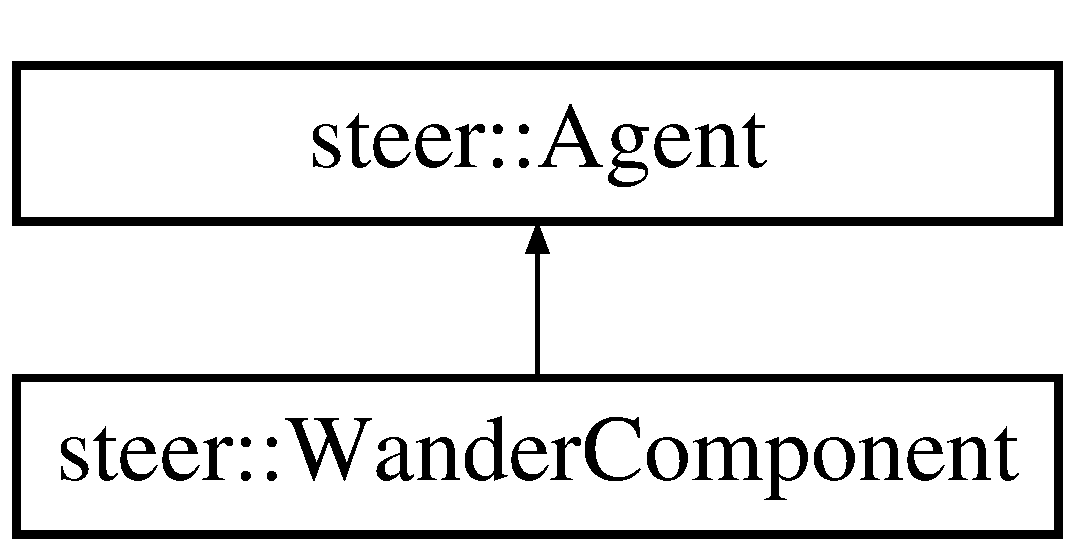
\includegraphics[height=2.000000cm]{classsteer_1_1_wander_component}
\end{center}
\end{figure}
\subsection*{Public Member Functions}
\begin{DoxyCompactItemize}
\item 
\hypertarget{classsteer_1_1_wander_component_aac30556d156d8f7dc1bae57ac8919148}{{\bfseries Wander\-Component} (\hyperlink{structsteer_1_1_behavior_parameters}{steer\-::\-Behavior\-Parameters} $\ast$params)}\label{classsteer_1_1_wander_component_aac30556d156d8f7dc1bae57ac8919148}

\item 
\hypertarget{classsteer_1_1_wander_component_a6f4e2b363c300c5cf372c14d733fef1f}{void {\bfseries Update} (float dt)}\label{classsteer_1_1_wander_component_a6f4e2b363c300c5cf372c14d733fef1f}

\item 
void \hyperlink{classsteer_1_1_wander_component_a395f1351ae56b347b9b369853ff3f81d}{set\-Weight} (const float weight)
\begin{DoxyCompactList}\small\item\em Set the value of the weight multiplier for the seek component. \end{DoxyCompactList}\item 
\hypertarget{classsteer_1_1_wander_component_ade044e7fe51d92ea53101c41a480bb34}{float \hyperlink{classsteer_1_1_wander_component_ade044e7fe51d92ea53101c41a480bb34}{get\-Weight} () const }\label{classsteer_1_1_wander_component_ade044e7fe51d92ea53101c41a480bb34}

\begin{DoxyCompactList}\small\item\em Get the value of the weight multiplier for the seek component. \end{DoxyCompactList}\item 
\hypertarget{classsteer_1_1_wander_component_a35dbaf830f2a1771b89168cf0e5d3ddf}{void \hyperlink{classsteer_1_1_wander_component_a35dbaf830f2a1771b89168cf0e5d3ddf}{set\-Rotation} (float r)}\label{classsteer_1_1_wander_component_a35dbaf830f2a1771b89168cf0e5d3ddf}

\begin{DoxyCompactList}\small\item\em Set the value of the seek component rotation. \end{DoxyCompactList}\item 
\hypertarget{classsteer_1_1_wander_component_afaeb73f4dc652cdacf8222989088bb9b}{float \hyperlink{classsteer_1_1_wander_component_afaeb73f4dc652cdacf8222989088bb9b}{get\-Rotation} ()}\label{classsteer_1_1_wander_component_afaeb73f4dc652cdacf8222989088bb9b}

\begin{DoxyCompactList}\small\item\em Get the value of the seek component rotation. \end{DoxyCompactList}\item 
virtual bool \hyperlink{classsteer_1_1_wander_component_abf53f90d185d86aebf2cb744fac59f37}{on} (\hyperlink{namespacesteer_afe6e72f8f8088962727051501181acbe}{steer\-::behavior\-Type} behavior)
\begin{DoxyCompactList}\small\item\em This pure virtual function tests if a specific bit of m\-\_\-i\-Flags is set using bitwise operations. Must be overridden in derived classes. \end{DoxyCompactList}\item 
\hypertarget{classsteer_1_1_wander_component_ac2f9e2a98cf68d628bec4e9a927a7423}{void {\bfseries wander\-On} ()}\label{classsteer_1_1_wander_component_ac2f9e2a98cf68d628bec4e9a927a7423}

\item 
\hypertarget{classsteer_1_1_wander_component_ad880ef234fcdfa926776f45b760e54c3}{void {\bfseries wander\-Off} ()}\label{classsteer_1_1_wander_component_ad880ef234fcdfa926776f45b760e54c3}

\item 
\hypertarget{classsteer_1_1_wander_component_af0be348a7d446704817061359c6053f7}{bool {\bfseries is\-Wander\-On} ()}\label{classsteer_1_1_wander_component_af0be348a7d446704817061359c6053f7}

\item 
\hypertarget{classsteer_1_1_wander_component_ab46e62ab424633354ce4eca25803caab}{virtual \hyperlink{structsteer_1_1_vector2}{Vector2} \hyperlink{classsteer_1_1_wander_component_ab46e62ab424633354ce4eca25803caab}{Calculate} ()}\label{classsteer_1_1_wander_component_ab46e62ab424633354ce4eca25803caab}

\begin{DoxyCompactList}\small\item\em A pure virtual method for calculating the steering vector. \end{DoxyCompactList}\end{DoxyCompactItemize}
\subsection*{Additional Inherited Members}


\subsection{Detailed Description}
An example implementation of the wander steering behavior. 

\subsection{Member Function Documentation}
\hypertarget{classsteer_1_1_wander_component_abf53f90d185d86aebf2cb744fac59f37}{\index{steer\-::\-Wander\-Component@{steer\-::\-Wander\-Component}!on@{on}}
\index{on@{on}!steer::WanderComponent@{steer\-::\-Wander\-Component}}
\subsubsection[{on}]{\setlength{\rightskip}{0pt plus 5cm}virtual bool steer\-::\-Wander\-Component\-::on (
\begin{DoxyParamCaption}
\item[{{\bf steer\-::behavior\-Type}}]{behavior}
\end{DoxyParamCaption}
)\hspace{0.3cm}{\ttfamily [inline]}, {\ttfamily [virtual]}}}\label{classsteer_1_1_wander_component_abf53f90d185d86aebf2cb744fac59f37}


This pure virtual function tests if a specific bit of m\-\_\-i\-Flags is set using bitwise operations. Must be overridden in derived classes. 


\begin{DoxyParams}{Parameters}
{\em behavior} & -\/ enum behavior\-Type. \\
\hline
\end{DoxyParams}


Implements \hyperlink{classsteer_1_1_agent_a707204e49e6519c7a8ea0f3ded608d98}{steer\-::\-Agent}.

\hypertarget{classsteer_1_1_wander_component_a395f1351ae56b347b9b369853ff3f81d}{\index{steer\-::\-Wander\-Component@{steer\-::\-Wander\-Component}!set\-Weight@{set\-Weight}}
\index{set\-Weight@{set\-Weight}!steer::WanderComponent@{steer\-::\-Wander\-Component}}
\subsubsection[{set\-Weight}]{\setlength{\rightskip}{0pt plus 5cm}void steer\-::\-Wander\-Component\-::set\-Weight (
\begin{DoxyParamCaption}
\item[{const float}]{weight}
\end{DoxyParamCaption}
)\hspace{0.3cm}{\ttfamily [inline]}}}\label{classsteer_1_1_wander_component_a395f1351ae56b347b9b369853ff3f81d}


Set the value of the weight multiplier for the seek component. 


\begin{DoxyParams}{Parameters}
{\em weight} & -\/ a plain old float. \\
\hline
\end{DoxyParams}


The documentation for this class was generated from the following files\-:\begin{DoxyCompactItemize}
\item 
include/steeriously/components/Wander\-Component.\-hpp\item 
src/steeriously/components/Wander\-Component.\-cpp\end{DoxyCompactItemize}

\addcontentsline{toc}{part}{Index}
\printindex
\end{document}
